\chapter{Circuit simulations for generating various waveform signals}
% Outline the simulation results based on the chosen approach in the previous chapter
The circuit simulations are run to validate the behaviour of the conceptual design of the Riemann Pump. The simulated output signal already identifies some fundamental ideas to understand the drawbacks and trade-offs of the designed circuit.\\
To investigate the theoretical concepts of chapter \ref{ch:design} the harmonic balance simulator is used.
The harmonic balance simulation is done with the design tool \gls{ab:ads}.
The benefit of the harmonic balance simulation is that the whole system is modelled in a steady state mode, so that no transients influences the results. \textit{"Harmonic balance is a frequency-domain analysis technique for simulating non linear circuits and systems[...]"}  ADS\_Harmonic\_Balance.pdf\\
In a first step the analog signal across the output impedance in the time domain is plotted to check whether a signal could be synthesized or not. 
After various signals could be synthesized, a short stability and energy consumption analysis is done.
The stability check is needed to validate that the circuit do not oscillate.
As well the circuits energy consumption has to be checked if it is in a moderate range (\textit{which is the moderate range? mention it here?}) since it could be implemented in mobile devices.\\
    In the last step a simulation is run which makes the concept comparable to the realized circuit. 
   In this simulation the transistor dimensions are adapted to the dimension of the built demonstrator. 
   This should give an insight to the behaviour of the constructed demonstrator.\\
   It is important to note that all simulations are done under ideal conditions and hence no losses are taken into account. 
    The modelling and simulation of the designed circuit under real conditions considering all loss effects would go beyond the scope of this thesis. Therefore a keep it small and simple approach is chosen.\\   

\section{Generating various analog signals with digital input control}
The generation of analog signals at the output of the designed circuit is the purpose of this concept.
 The designed Riemann Pump should be able to create various (arbitrary) waveform signals by converting a digital bit sequence into the analog output signal.
 % Therefore the Riemann Pump is a arbitrary waveform generator and also a high speed digital-to-analog converter
%To validate the feasibility of the presented concept, a digital input control code is required.
%To get this code an approximation by hand is done since no algorithm exists which can compute this.
Simulations in time domain are required to validate the signal integrity of the synthesized signals since the output signals consist of the integration of current over time to charge a capacitor at the output.
 %Based on the idea, to integrate the current over time to charge a capacitor at the outputlinear approximation of current charging a capacitor, this would be the best way to verify its correctness.
  If the output signal is verified to be as good as wanted, a simulation in the frequency domain can show the spurious free dynamic range of the \gls{ab:dac}.\\
To synthesize a certain analog signal at the output the corresponding Riemann Code is needed.
Due to the fact that no algorithm exists which computes this Riemann Code, it is done manually.\\ 
 %The generation of the various analog output signals is based on the concept of chapter \ref{ch:design}. 
 The presented \gls{ab:dac} have a resolution of three bit and synthesizes signals with an \gls{ab:osr} of four. 
  The components used, are optimized with respect to the signal integrity. 
  The dimension of the used components are tuned while simulation to ensure the desired output signal.
  In contrast to this optimized components, chapter \ref{ch:ProofOfConceptWithExistingComponents} deals with the simulation done with real dimensions of the demonstrator components. 
  This simulation should give an insight to what is expected for the measurements.
 
\subsection{Sine wave generation in the time domain}
As known from basic signal processing lecture
%[Oppenheim, MIT, Signals and Systems Lecture \textit{http://ocw.mit.edu/resources/res-6-007-signals-and-systems-spring-2011/lecture-notes/MITRES\_6\_007S11\_lec02.pdf}]
[REF.?] the sine wave for continuous time is the elementary signal and therefore synthesized first. 
For the generation of this sine wave a corresponding Riemann Code is required which will be converted to the analog output signal.\\
This Riemann Code is generated by hand via an approximation of a sine wave with a sequence of eight different slopes.
This eight different slopes represents a three bit resolution of the \gls{ab:dac} while the sequence consists of eight sampling points which refer to the \gls{ab:osr} of four.\\
Figure \ref{fig:RiemannCodeGenerationSineWave} presents the sequence of slopes used to approximate a sine wave. 

%\begin{figure}[htb!]
%   \centering
%   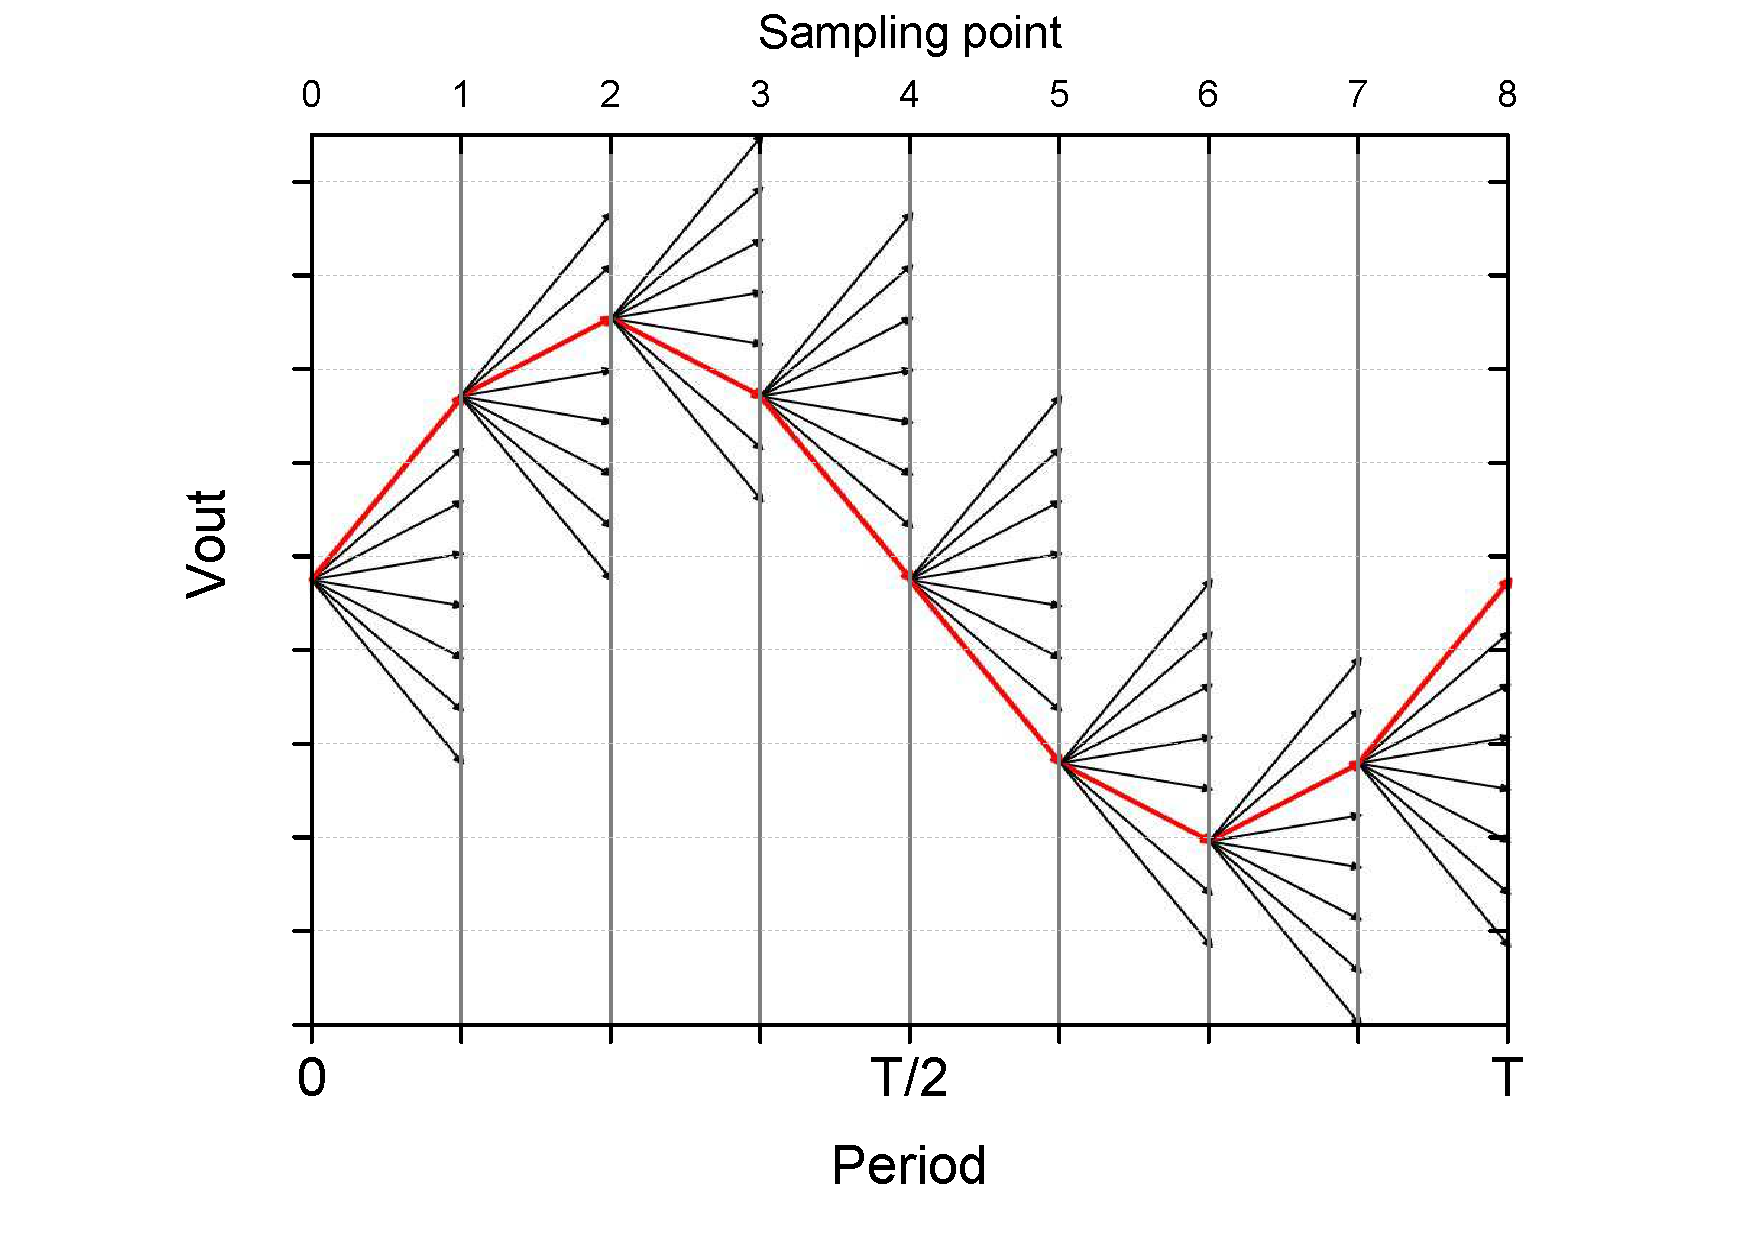
\includegraphics[width=0.75\textwidth]{RiemannCodeGeneration.pdf}
%   \caption{One possible approximation of sine wave generation to get the Riemann Code}
%   \label{fig:RiemannCodeGenerationSineWave}
%\end{figure}



\begin{figure}[htb!]
   \centering 
   %LaTeX with PSTricks extensions
%%Creator: 0.91_64bit
%%Please note this file requires PSTricks extensions
\psset{xunit=.5pt,yunit=.5pt,runit=.5pt}
\begin{pspicture}(389.76377953,265.7480315)
{
\newrgbcolor{curcolor}{0 0 0}
\pscustom[linestyle=none,fillstyle=solid,fillcolor=curcolor]
{
\newpath
\moveto(91.28064318,138.16043958)
\lineto(91.65492518,136.83539376)
\lineto(93.22690959,137.79393755)
\lineto(91.28064318,138.16043958)
}
}
{
\newrgbcolor{curcolor}{0 0 0}
\pscustom[linewidth=0.5549305,linecolor=curcolor]
{
\newpath
\moveto(91.28064318,138.16043958)
\lineto(91.65492518,136.83539376)
\lineto(93.22690959,137.79393755)
\lineto(91.28064318,138.16043958)
}
}
{
\newrgbcolor{curcolor}{0 0 0}
\pscustom[linewidth=0.5549305,linecolor=curcolor]
{
\newpath
\moveto(59.84095646,132.46555923)
\lineto(91.46778578,137.51201031)
}
}
{
\newrgbcolor{curcolor}{0 0 0}
\pscustom[linestyle=none,fillstyle=solid,fillcolor=curcolor]
{
\newpath
\moveto(91.65492704,128.09572646)
\lineto(91.28064503,126.77068065)
\lineto(93.22691145,127.16537514)
\lineto(91.65492704,128.09572646)
}
}
{
\newrgbcolor{curcolor}{0 0 0}
\pscustom[linewidth=0.5549305,linecolor=curcolor]
{
\newpath
\moveto(91.65492704,128.09572646)
\lineto(91.28064503,126.77068065)
\lineto(93.22691145,127.16537514)
\lineto(91.65492704,128.09572646)
}
}
{
\newrgbcolor{curcolor}{0 0 0}
\pscustom[linewidth=0.5549305,linecolor=curcolor]
{
\newpath
\moveto(59.84095646,132.46555923)
\lineto(91.46778578,127.44730061)
}
}
{
\newrgbcolor{curcolor}{0 0 0}
\pscustom[linestyle=none,fillstyle=solid,fillcolor=curcolor]
{
\newpath
\moveto(91.20579067,148.25334049)
\lineto(92.17892388,147.09744946)
\lineto(93.22691349,148.42249527)
\lineto(91.20579067,148.25334049)
}
}
{
\newrgbcolor{curcolor}{0 0 0}
\pscustom[linewidth=0.5549305,linecolor=curcolor]
{
\newpath
\moveto(91.20579067,148.25334049)
\lineto(92.17892388,147.09744946)
\lineto(93.22691349,148.42249527)
\lineto(91.20579067,148.25334049)
}
}
{
\newrgbcolor{curcolor}{0 0 0}
\pscustom[linewidth=0.5549305,linecolor=curcolor]
{
\newpath
\moveto(59.84095646,132.46555923)
\lineto(91.69235498,147.68948987)
}
}
{
\newrgbcolor{curcolor}{0 0 0}
\pscustom[linestyle=none,fillstyle=solid,fillcolor=curcolor]
{
\newpath
\moveto(91.31806943,158.51539702)
\lineto(92.62805644,157.5850457)
\lineto(93.22690765,159.05105384)
\lineto(91.31806943,158.51539702)
}
}
{
\newrgbcolor{curcolor}{0 0 0}
\pscustom[linewidth=0.5549305,linecolor=curcolor]
{
\newpath
\moveto(91.31806943,158.51539702)
\lineto(92.62805644,157.5850457)
\lineto(93.22690765,159.05105384)
\lineto(91.31806943,158.51539702)
}
}
{
\newrgbcolor{curcolor}{0 0 0}
\pscustom[linewidth=0.5549305,linecolor=curcolor]
{
\newpath
\moveto(59.84095646,132.46555923)
\lineto(91.99178058,158.06431667)
}
}
{
\newrgbcolor{curcolor}{0 0 0}
\pscustom[linestyle=none,fillstyle=solid,fillcolor=curcolor]
{
\newpath
\moveto(92.17892018,117.83366993)
\lineto(91.20578697,116.6777789)
\lineto(93.22690979,116.53681658)
\lineto(92.17892018,117.83366993)
}
}
{
\newrgbcolor{curcolor}{0 0 0}
\pscustom[linewidth=0.5549305,linecolor=curcolor]
{
\newpath
\moveto(92.17892018,117.83366993)
\lineto(91.20578697,116.6777789)
\lineto(93.22690979,116.53681658)
\lineto(92.17892018,117.83366993)
}
}
{
\newrgbcolor{curcolor}{0 0 0}
\pscustom[linewidth=0.5549305,linecolor=curcolor]
{
\newpath
\moveto(59.84095646,132.46555923)
\lineto(91.69235498,117.2416286)
}
}
{
\newrgbcolor{curcolor}{0 0 0}
\pscustom[linestyle=none,fillstyle=solid,fillcolor=curcolor]
{
\newpath
\moveto(92.62805655,107.34607578)
\lineto(91.31806954,106.41572446)
\lineto(93.22690776,105.88006764)
\lineto(92.62805655,107.34607578)
}
}
{
\newrgbcolor{curcolor}{0 0 0}
\pscustom[linewidth=0.5549305,linecolor=curcolor]
{
\newpath
\moveto(92.62805655,107.34607578)
\lineto(91.31806954,106.41572446)
\lineto(93.22690776,105.88006764)
\lineto(92.62805655,107.34607578)
}
}
{
\newrgbcolor{curcolor}{0 0 0}
\pscustom[linewidth=0.5549305,linecolor=curcolor]
{
\newpath
\moveto(59.84095646,132.46555923)
\lineto(91.99178058,106.89499426)
}
}
{
\newrgbcolor{curcolor}{0 0 0}
\pscustom[linestyle=none,fillstyle=solid,fillcolor=curcolor]
{
\newpath
\moveto(92.9649099,96.77390221)
\lineto(91.46778188,96.01270567)
\lineto(93.2269073,95.25150914)
\lineto(92.9649099,96.77390221)
}
}
{
\newrgbcolor{curcolor}{0 0 0}
\pscustom[linewidth=0.5549305,linecolor=curcolor]
{
\newpath
\moveto(92.9649099,96.77390221)
\lineto(91.46778188,96.01270567)
\lineto(93.2269073,95.25150914)
\lineto(92.9649099,96.77390221)
}
}
{
\newrgbcolor{curcolor}{0 0 0}
\pscustom[linewidth=0.5549305,linecolor=curcolor]
{
\newpath
\moveto(59.84095646,132.46555923)
\lineto(92.21634979,96.4073976)
}
}
{
\newrgbcolor{curcolor}{1 0 0}
\pscustom[linestyle=none,fillstyle=solid,fillcolor=curcolor]
{
\newpath
\moveto(91.46778297,168.91841175)
\lineto(92.96491099,168.15721522)
\lineto(93.22690839,169.67960828)
\lineto(91.46778297,168.91841175)
}
}
{
\newrgbcolor{curcolor}{1 0 0}
\pscustom[linewidth=1.109861,linecolor=curcolor]
{
\newpath
\moveto(91.46778297,168.91841175)
\lineto(92.96491099,168.15721522)
\lineto(93.22690839,169.67960828)
\lineto(91.46778297,168.91841175)
}
}
{
\newrgbcolor{curcolor}{1 0 0}
\pscustom[linewidth=1.109861,linecolor=curcolor]
{
\newpath
\moveto(59.84095646,132.46555923)
\lineto(92.21634979,168.55191333)
}
}
{
\newrgbcolor{curcolor}{0 0 0}
\pscustom[linestyle=none,fillstyle=solid,fillcolor=curcolor]
{
\newpath
\moveto(124.18003482,175.37449081)
\lineto(124.55431682,174.04944499)
\lineto(126.12630124,174.97979631)
\lineto(124.18003482,175.37449081)
}
}
{
\newrgbcolor{curcolor}{0 0 0}
\pscustom[linewidth=0.5549305,linecolor=curcolor]
{
\newpath
\moveto(124.18003482,175.37449081)
\lineto(124.55431682,174.04944499)
\lineto(126.12630124,174.97979631)
\lineto(124.18003482,175.37449081)
}
}
{
\newrgbcolor{curcolor}{0 0 0}
\pscustom[linewidth=0.5549305,linecolor=curcolor]
{
\newpath
\moveto(92.74033958,169.67961046)
\lineto(124.3671689,174.69786907)
}
}
{
\newrgbcolor{curcolor}{0 0 0}
\pscustom[linestyle=none,fillstyle=solid,fillcolor=curcolor]
{
\newpath
\moveto(124.55431442,165.30978411)
\lineto(124.18003241,163.98473829)
\lineto(126.12629883,164.35124033)
\lineto(124.55431442,165.30978411)
}
}
{
\newrgbcolor{curcolor}{0 0 0}
\pscustom[linewidth=0.5549305,linecolor=curcolor]
{
\newpath
\moveto(124.55431442,165.30978411)
\lineto(124.18003241,163.98473829)
\lineto(126.12629883,164.35124033)
\lineto(124.55431442,165.30978411)
}
}
{
\newrgbcolor{curcolor}{0 0 0}
\pscustom[linewidth=0.5549305,linecolor=curcolor]
{
\newpath
\moveto(92.74033958,169.67961046)
\lineto(124.3671689,164.63315938)
}
}
{
\newrgbcolor{curcolor}{1 0 0}
\pscustom[linestyle=none,fillstyle=solid,fillcolor=curcolor]
{
\newpath
\moveto(124.10516952,185.46739492)
\lineto(125.07830273,184.31150389)
\lineto(126.12629234,185.63654971)
\lineto(124.10516952,185.46739492)
}
}
{
\newrgbcolor{curcolor}{1 0 0}
\pscustom[linewidth=1.109861,linecolor=curcolor]
{
\newpath
\moveto(124.10516952,185.46739492)
\lineto(125.07830273,184.31150389)
\lineto(126.12629234,185.63654971)
\lineto(124.10516952,185.46739492)
}
}
{
\newrgbcolor{curcolor}{1 0 0}
\pscustom[linewidth=1.109861,linecolor=curcolor]
{
\newpath
\moveto(92.74033958,169.67961046)
\lineto(124.5917381,184.90354109)
}
}
{
\newrgbcolor{curcolor}{0 0 0}
\pscustom[linestyle=none,fillstyle=solid,fillcolor=curcolor]
{
\newpath
\moveto(124.21746107,195.72944503)
\lineto(125.52744809,194.79909372)
\lineto(126.12629929,196.26510185)
\lineto(124.21746107,195.72944503)
}
}
{
\newrgbcolor{curcolor}{0 0 0}
\pscustom[linewidth=0.5549305,linecolor=curcolor]
{
\newpath
\moveto(124.21746107,195.72944503)
\lineto(125.52744809,194.79909372)
\lineto(126.12629929,196.26510185)
\lineto(124.21746107,195.72944503)
}
}
{
\newrgbcolor{curcolor}{0 0 0}
\pscustom[linewidth=0.5549305,linecolor=curcolor]
{
\newpath
\moveto(92.74033958,169.67961046)
\lineto(124.8911637,195.25017543)
}
}
{
\newrgbcolor{curcolor}{0 0 0}
\pscustom[linestyle=none,fillstyle=solid,fillcolor=curcolor]
{
\newpath
\moveto(125.07829904,155.04772116)
\lineto(124.10516583,153.89183013)
\lineto(126.12628865,153.72267534)
\lineto(125.07829904,155.04772116)
}
}
{
\newrgbcolor{curcolor}{0 0 0}
\pscustom[linewidth=0.5549305,linecolor=curcolor]
{
\newpath
\moveto(125.07829904,155.04772116)
\lineto(124.10516583,153.89183013)
\lineto(126.12628865,153.72267534)
\lineto(125.07829904,155.04772116)
}
}
{
\newrgbcolor{curcolor}{0 0 0}
\pscustom[linewidth=0.5549305,linecolor=curcolor]
{
\newpath
\moveto(92.74033958,169.67961046)
\lineto(124.5917381,154.45567982)
}
}
{
\newrgbcolor{curcolor}{0 0 0}
\pscustom[linestyle=none,fillstyle=solid,fillcolor=curcolor]
{
\newpath
\moveto(125.52744394,144.56013021)
\lineto(124.21745692,143.6297789)
\lineto(126.12629514,143.09412208)
\lineto(125.52744394,144.56013021)
}
}
{
\newrgbcolor{curcolor}{0 0 0}
\pscustom[linewidth=0.5549305,linecolor=curcolor]
{
\newpath
\moveto(125.52744394,144.56013021)
\lineto(124.21745692,143.6297789)
\lineto(126.12629514,143.09412208)
\lineto(125.52744394,144.56013021)
}
}
{
\newrgbcolor{curcolor}{0 0 0}
\pscustom[linewidth=0.5549305,linecolor=curcolor]
{
\newpath
\moveto(92.74033958,169.67961046)
\lineto(124.8911637,144.08085302)
}
}
{
\newrgbcolor{curcolor}{0 0 0}
\pscustom[linestyle=none,fillstyle=solid,fillcolor=curcolor]
{
\newpath
\moveto(125.86430154,133.98795343)
\lineto(124.36717353,133.2267569)
\lineto(126.12629895,132.46556037)
\lineto(125.86430154,133.98795343)
}
}
{
\newrgbcolor{curcolor}{0 0 0}
\pscustom[linewidth=0.5549305,linecolor=curcolor]
{
\newpath
\moveto(125.86430154,133.98795343)
\lineto(124.36717353,133.2267569)
\lineto(126.12629895,132.46556037)
\lineto(125.86430154,133.98795343)
}
}
{
\newrgbcolor{curcolor}{0 0 0}
\pscustom[linewidth=0.5549305,linecolor=curcolor]
{
\newpath
\moveto(92.74033958,169.67961046)
\lineto(125.11573291,133.59325636)
}
}
{
\newrgbcolor{curcolor}{0 0 0}
\pscustom[linestyle=none,fillstyle=solid,fillcolor=curcolor]
{
\newpath
\moveto(124.36717036,206.13246619)
\lineto(125.86429837,205.37126966)
\lineto(126.12629577,206.89366272)
\lineto(124.36717036,206.13246619)
}
}
{
\newrgbcolor{curcolor}{0 0 0}
\pscustom[linewidth=0.5549305,linecolor=curcolor]
{
\newpath
\moveto(124.36717036,206.13246619)
\lineto(125.86429837,205.37126966)
\lineto(126.12629577,206.89366272)
\lineto(124.36717036,206.13246619)
}
}
{
\newrgbcolor{curcolor}{0 0 0}
\pscustom[linewidth=0.5549305,linecolor=curcolor]
{
\newpath
\moveto(92.74033958,169.67961046)
\lineto(125.11573291,205.76596456)
}
}
{
\newrgbcolor{curcolor}{0 0 0}
\pscustom[linestyle=none,fillstyle=solid,fillcolor=curcolor]
{
\newpath
\moveto(157.56598056,191.19046948)
\lineto(157.94026257,189.86542367)
\lineto(159.51224698,190.82396745)
\lineto(157.56598056,191.19046948)
}
}
{
\newrgbcolor{curcolor}{0 0 0}
\pscustom[linewidth=0.5549305,linecolor=curcolor]
{
\newpath
\moveto(157.56598056,191.19046948)
\lineto(157.94026257,189.86542367)
\lineto(159.51224698,190.82396745)
\lineto(157.56598056,191.19046948)
}
}
{
\newrgbcolor{curcolor}{0 0 0}
\pscustom[linewidth=0.5549305,linecolor=curcolor]
{
\newpath
\moveto(126.12629811,185.49558271)
\lineto(157.75312743,190.54203379)
}
}
{
\newrgbcolor{curcolor}{0 0 0}
\pscustom[linestyle=none,fillstyle=solid,fillcolor=curcolor]
{
\newpath
\moveto(157.94026869,181.12574994)
\lineto(157.56598669,179.80070413)
\lineto(159.51225311,180.16720616)
\lineto(157.94026869,181.12574994)
}
}
{
\newrgbcolor{curcolor}{0 0 0}
\pscustom[linewidth=0.5549305,linecolor=curcolor]
{
\newpath
\moveto(157.94026869,181.12574994)
\lineto(157.56598669,179.80070413)
\lineto(159.51225311,180.16720616)
\lineto(157.94026869,181.12574994)
}
}
{
\newrgbcolor{curcolor}{0 0 0}
\pscustom[linewidth=0.5549305,linecolor=curcolor]
{
\newpath
\moveto(126.12629811,185.49558271)
\lineto(157.75312743,180.44913163)
}
}
{
\newrgbcolor{curcolor}{0 0 0}
\pscustom[linestyle=none,fillstyle=solid,fillcolor=curcolor]
{
\newpath
\moveto(157.49113232,201.28336718)
\lineto(158.46426553,200.12747615)
\lineto(159.51225514,201.45252196)
\lineto(157.49113232,201.28336718)
}
}
{
\newrgbcolor{curcolor}{0 0 0}
\pscustom[linewidth=0.5549305,linecolor=curcolor]
{
\newpath
\moveto(157.49113232,201.28336718)
\lineto(158.46426553,200.12747615)
\lineto(159.51225514,201.45252196)
\lineto(157.49113232,201.28336718)
}
}
{
\newrgbcolor{curcolor}{0 0 0}
\pscustom[linewidth=0.5549305,linecolor=curcolor]
{
\newpath
\moveto(126.12629811,185.49558271)
\lineto(157.97769663,200.71951335)
}
}
{
\newrgbcolor{curcolor}{0 0 0}
\pscustom[linestyle=none,fillstyle=solid,fillcolor=curcolor]
{
\newpath
\moveto(157.60341961,211.54542371)
\lineto(158.91340662,210.61507239)
\lineto(159.51225783,212.08108053)
\lineto(157.60341961,211.54542371)
}
}
{
\newrgbcolor{curcolor}{0 0 0}
\pscustom[linewidth=0.5549305,linecolor=curcolor]
{
\newpath
\moveto(157.60341961,211.54542371)
\lineto(158.91340662,210.61507239)
\lineto(159.51225783,212.08108053)
\lineto(157.60341961,211.54542371)
}
}
{
\newrgbcolor{curcolor}{0 0 0}
\pscustom[linewidth=0.5549305,linecolor=curcolor]
{
\newpath
\moveto(126.12629811,185.49558271)
\lineto(158.27712224,211.09434015)
}
}
{
\newrgbcolor{curcolor}{1 0 0}
\pscustom[linestyle=none,fillstyle=solid,fillcolor=curcolor]
{
\newpath
\moveto(158.46426183,170.86369341)
\lineto(157.49112862,169.70780238)
\lineto(159.51225144,169.5386476)
\lineto(158.46426183,170.86369341)
}
}
{
\newrgbcolor{curcolor}{1 0 0}
\pscustom[linewidth=1.109861,linecolor=curcolor]
{
\newpath
\moveto(158.46426183,170.86369341)
\lineto(157.49112862,169.70780238)
\lineto(159.51225144,169.5386476)
\lineto(158.46426183,170.86369341)
}
}
{
\newrgbcolor{curcolor}{1 0 0}
\pscustom[linewidth=1.109861,linecolor=curcolor]
{
\newpath
\moveto(126.12629811,185.49558271)
\lineto(157.97769663,170.27165208)
}
}
{
\newrgbcolor{curcolor}{0 0 0}
\pscustom[linestyle=none,fillstyle=solid,fillcolor=curcolor]
{
\newpath
\moveto(158.91339821,160.37610247)
\lineto(157.60341119,159.44575115)
\lineto(159.51224941,158.91009433)
\lineto(158.91339821,160.37610247)
}
}
{
\newrgbcolor{curcolor}{0 0 0}
\pscustom[linewidth=0.5549305,linecolor=curcolor]
{
\newpath
\moveto(158.91339821,160.37610247)
\lineto(157.60341119,159.44575115)
\lineto(159.51224941,158.91009433)
\lineto(158.91339821,160.37610247)
}
}
{
\newrgbcolor{curcolor}{0 0 0}
\pscustom[linewidth=0.5549305,linecolor=curcolor]
{
\newpath
\moveto(126.12629811,185.49558271)
\lineto(158.27712224,159.89682527)
}
}
{
\newrgbcolor{curcolor}{0 0 0}
\pscustom[linestyle=none,fillstyle=solid,fillcolor=curcolor]
{
\newpath
\moveto(159.25025581,149.8039289)
\lineto(157.7531278,149.04273236)
\lineto(159.51225322,148.28153583)
\lineto(159.25025581,149.8039289)
}
}
{
\newrgbcolor{curcolor}{0 0 0}
\pscustom[linewidth=0.5549305,linecolor=curcolor]
{
\newpath
\moveto(159.25025581,149.8039289)
\lineto(157.7531278,149.04273236)
\lineto(159.51225322,148.28153583)
\lineto(159.25025581,149.8039289)
}
}
{
\newrgbcolor{curcolor}{0 0 0}
\pscustom[linewidth=0.5549305,linecolor=curcolor]
{
\newpath
\moveto(126.12629811,185.49558271)
\lineto(158.50169144,149.40922861)
}
}
{
\newrgbcolor{curcolor}{0 0 0}
\pscustom[linestyle=none,fillstyle=solid,fillcolor=curcolor]
{
\newpath
\moveto(157.75312463,221.94844486)
\lineto(159.25025264,221.18724833)
\lineto(159.51225004,222.7096414)
\lineto(157.75312463,221.94844486)
}
}
{
\newrgbcolor{curcolor}{0 0 0}
\pscustom[linewidth=0.5549305,linecolor=curcolor]
{
\newpath
\moveto(157.75312463,221.94844486)
\lineto(159.25025264,221.18724833)
\lineto(159.51225004,222.7096414)
\lineto(157.75312463,221.94844486)
}
}
{
\newrgbcolor{curcolor}{0 0 0}
\pscustom[linewidth=0.5549305,linecolor=curcolor]
{
\newpath
\moveto(126.12629811,185.49558271)
\lineto(158.50169144,221.58193681)
}
}
{
\newrgbcolor{curcolor}{0 0 0}
\pscustom[linestyle=none,fillstyle=solid,fillcolor=curcolor]
{
\newpath
\moveto(190.46537647,175.37449081)
\lineto(190.83965848,174.04944499)
\lineto(192.41164289,174.97979631)
\lineto(190.46537647,175.37449081)
}
}
{
\newrgbcolor{curcolor}{0 0 0}
\pscustom[linewidth=0.5549305,linecolor=curcolor]
{
\newpath
\moveto(190.46537647,175.37449081)
\lineto(190.83965848,174.04944499)
\lineto(192.41164289,174.97979631)
\lineto(190.46537647,175.37449081)
}
}
{
\newrgbcolor{curcolor}{0 0 0}
\pscustom[linewidth=0.5549305,linecolor=curcolor]
{
\newpath
\moveto(159.02568976,169.67961046)
\lineto(190.65251908,174.69786907)
}
}
{
\newrgbcolor{curcolor}{0 0 0}
\pscustom[linestyle=none,fillstyle=solid,fillcolor=curcolor]
{
\newpath
\moveto(190.83966033,165.30978411)
\lineto(190.46537833,163.98473829)
\lineto(192.41164475,164.35124033)
\lineto(190.83966033,165.30978411)
}
}
{
\newrgbcolor{curcolor}{0 0 0}
\pscustom[linewidth=0.5549305,linecolor=curcolor]
{
\newpath
\moveto(190.83966033,165.30978411)
\lineto(190.46537833,163.98473829)
\lineto(192.41164475,164.35124033)
\lineto(190.83966033,165.30978411)
}
}
{
\newrgbcolor{curcolor}{0 0 0}
\pscustom[linewidth=0.5549305,linecolor=curcolor]
{
\newpath
\moveto(159.02568976,169.67961046)
\lineto(190.65251908,164.63315938)
}
}
{
\newrgbcolor{curcolor}{0 0 0}
\pscustom[linestyle=none,fillstyle=solid,fillcolor=curcolor]
{
\newpath
\moveto(190.39052396,185.46739492)
\lineto(191.36365717,184.31150389)
\lineto(192.41164678,185.63654971)
\lineto(190.39052396,185.46739492)
}
}
{
\newrgbcolor{curcolor}{0 0 0}
\pscustom[linewidth=0.5549305,linecolor=curcolor]
{
\newpath
\moveto(190.39052396,185.46739492)
\lineto(191.36365717,184.31150389)
\lineto(192.41164678,185.63654971)
\lineto(190.39052396,185.46739492)
}
}
{
\newrgbcolor{curcolor}{0 0 0}
\pscustom[linewidth=0.5549305,linecolor=curcolor]
{
\newpath
\moveto(159.02568976,169.67961046)
\lineto(190.87708828,184.90354109)
}
}
{
\newrgbcolor{curcolor}{0 0 0}
\pscustom[linestyle=none,fillstyle=solid,fillcolor=curcolor]
{
\newpath
\moveto(190.50279846,195.72944503)
\lineto(191.81278548,194.79909372)
\lineto(192.41163668,196.26510185)
\lineto(190.50279846,195.72944503)
}
}
{
\newrgbcolor{curcolor}{0 0 0}
\pscustom[linewidth=0.5549305,linecolor=curcolor]
{
\newpath
\moveto(190.50279846,195.72944503)
\lineto(191.81278548,194.79909372)
\lineto(192.41163668,196.26510185)
\lineto(190.50279846,195.72944503)
}
}
{
\newrgbcolor{curcolor}{0 0 0}
\pscustom[linewidth=0.5549305,linecolor=curcolor]
{
\newpath
\moveto(159.02568976,169.67961046)
\lineto(191.17651388,195.25017543)
}
}
{
\newrgbcolor{curcolor}{0 0 0}
\pscustom[linestyle=none,fillstyle=solid,fillcolor=curcolor]
{
\newpath
\moveto(191.36365348,155.04772116)
\lineto(190.39052027,153.89183013)
\lineto(192.41164309,153.72267534)
\lineto(191.36365348,155.04772116)
}
}
{
\newrgbcolor{curcolor}{0 0 0}
\pscustom[linewidth=0.5549305,linecolor=curcolor]
{
\newpath
\moveto(191.36365348,155.04772116)
\lineto(190.39052027,153.89183013)
\lineto(192.41164309,153.72267534)
\lineto(191.36365348,155.04772116)
}
}
{
\newrgbcolor{curcolor}{0 0 0}
\pscustom[linewidth=0.5549305,linecolor=curcolor]
{
\newpath
\moveto(159.02568976,169.67961046)
\lineto(190.87708828,154.45567982)
}
}
{
\newrgbcolor{curcolor}{0 0 0}
\pscustom[linestyle=none,fillstyle=solid,fillcolor=curcolor]
{
\newpath
\moveto(191.81278985,144.56013021)
\lineto(190.50280284,143.6297789)
\lineto(192.41164106,143.09412208)
\lineto(191.81278985,144.56013021)
}
}
{
\newrgbcolor{curcolor}{0 0 0}
\pscustom[linewidth=0.5549305,linecolor=curcolor]
{
\newpath
\moveto(191.81278985,144.56013021)
\lineto(190.50280284,143.6297789)
\lineto(192.41164106,143.09412208)
\lineto(191.81278985,144.56013021)
}
}
{
\newrgbcolor{curcolor}{0 0 0}
\pscustom[linewidth=0.5549305,linecolor=curcolor]
{
\newpath
\moveto(159.02568976,169.67961046)
\lineto(191.17651388,144.08085302)
}
}
{
\newrgbcolor{curcolor}{1 0 0}
\pscustom[linestyle=none,fillstyle=solid,fillcolor=curcolor]
{
\newpath
\moveto(192.14964319,133.98795343)
\lineto(190.65251518,133.2267569)
\lineto(192.4116406,132.46556037)
\lineto(192.14964319,133.98795343)
}
}
{
\newrgbcolor{curcolor}{1 0 0}
\pscustom[linewidth=1.109861,linecolor=curcolor]
{
\newpath
\moveto(192.14964319,133.98795343)
\lineto(190.65251518,133.2267569)
\lineto(192.4116406,132.46556037)
\lineto(192.14964319,133.98795343)
}
}
{
\newrgbcolor{curcolor}{1 0 0}
\pscustom[linewidth=1.109861,linecolor=curcolor]
{
\newpath
\moveto(159.02568976,169.67961046)
\lineto(191.40108308,133.59325636)
}
}
{
\newrgbcolor{curcolor}{0 0 0}
\pscustom[linestyle=none,fillstyle=solid,fillcolor=curcolor]
{
\newpath
\moveto(190.65251627,206.13246619)
\lineto(192.14964429,205.37126966)
\lineto(192.41164169,206.89366272)
\lineto(190.65251627,206.13246619)
}
}
{
\newrgbcolor{curcolor}{0 0 0}
\pscustom[linewidth=0.5549305,linecolor=curcolor]
{
\newpath
\moveto(190.65251627,206.13246619)
\lineto(192.14964429,205.37126966)
\lineto(192.41164169,206.89366272)
\lineto(190.65251627,206.13246619)
}
}
{
\newrgbcolor{curcolor}{0 0 0}
\pscustom[linewidth=0.5549305,linecolor=curcolor]
{
\newpath
\moveto(159.02568976,169.67961046)
\lineto(191.40108308,205.76596456)
}
}
{
\newrgbcolor{curcolor}{0 0 0}
\pscustom[linestyle=none,fillstyle=solid,fillcolor=curcolor]
{
\newpath
\moveto(223.36476812,138.16043958)
\lineto(223.73905012,136.83539376)
\lineto(225.31103453,137.79393755)
\lineto(223.36476812,138.16043958)
}
}
{
\newrgbcolor{curcolor}{0 0 0}
\pscustom[linewidth=0.5549305,linecolor=curcolor]
{
\newpath
\moveto(223.36476812,138.16043958)
\lineto(223.73905012,136.83539376)
\lineto(225.31103453,137.79393755)
\lineto(223.36476812,138.16043958)
}
}
{
\newrgbcolor{curcolor}{0 0 0}
\pscustom[linewidth=0.5549305,linecolor=curcolor]
{
\newpath
\moveto(191.92507288,132.46555923)
\lineto(223.55190219,137.51201031)
}
}
{
\newrgbcolor{curcolor}{0 0 0}
\pscustom[linestyle=none,fillstyle=solid,fillcolor=curcolor]
{
\newpath
\moveto(223.73904345,128.09572646)
\lineto(223.36476145,126.77068065)
\lineto(225.31102787,127.16537514)
\lineto(223.73904345,128.09572646)
}
}
{
\newrgbcolor{curcolor}{0 0 0}
\pscustom[linewidth=0.5549305,linecolor=curcolor]
{
\newpath
\moveto(223.73904345,128.09572646)
\lineto(223.36476145,126.77068065)
\lineto(225.31102787,127.16537514)
\lineto(223.73904345,128.09572646)
}
}
{
\newrgbcolor{curcolor}{0 0 0}
\pscustom[linewidth=0.5549305,linecolor=curcolor]
{
\newpath
\moveto(191.92507288,132.46555923)
\lineto(223.55190219,127.44730061)
}
}
{
\newrgbcolor{curcolor}{0 0 0}
\pscustom[linestyle=none,fillstyle=solid,fillcolor=curcolor]
{
\newpath
\moveto(223.28990282,148.25334049)
\lineto(224.26303603,147.09744946)
\lineto(225.31102564,148.42249527)
\lineto(223.28990282,148.25334049)
}
}
{
\newrgbcolor{curcolor}{0 0 0}
\pscustom[linewidth=0.5549305,linecolor=curcolor]
{
\newpath
\moveto(223.28990282,148.25334049)
\lineto(224.26303603,147.09744946)
\lineto(225.31102564,148.42249527)
\lineto(223.28990282,148.25334049)
}
}
{
\newrgbcolor{curcolor}{0 0 0}
\pscustom[linewidth=0.5549305,linecolor=curcolor]
{
\newpath
\moveto(191.92507288,132.46555923)
\lineto(223.7764714,147.68948987)
}
}
{
\newrgbcolor{curcolor}{0 0 0}
\pscustom[linestyle=none,fillstyle=solid,fillcolor=curcolor]
{
\newpath
\moveto(223.40219437,158.51539702)
\lineto(224.74960958,157.5850457)
\lineto(225.31103259,159.05105384)
\lineto(223.40219437,158.51539702)
}
}
{
\newrgbcolor{curcolor}{0 0 0}
\pscustom[linewidth=0.5549305,linecolor=curcolor]
{
\newpath
\moveto(223.40219437,158.51539702)
\lineto(224.74960958,157.5850457)
\lineto(225.31103259,159.05105384)
\lineto(223.40219437,158.51539702)
}
}
{
\newrgbcolor{curcolor}{0 0 0}
\pscustom[linewidth=0.5549305,linecolor=curcolor]
{
\newpath
\moveto(191.92507288,132.46555923)
\lineto(224.075897,158.06431667)
}
}
{
\newrgbcolor{curcolor}{0 0 0}
\pscustom[linestyle=none,fillstyle=solid,fillcolor=curcolor]
{
\newpath
\moveto(224.26303233,117.83366993)
\lineto(223.28989912,116.6777789)
\lineto(225.31102194,116.53681658)
\lineto(224.26303233,117.83366993)
}
}
{
\newrgbcolor{curcolor}{0 0 0}
\pscustom[linewidth=0.5549305,linecolor=curcolor]
{
\newpath
\moveto(224.26303233,117.83366993)
\lineto(223.28989912,116.6777789)
\lineto(225.31102194,116.53681658)
\lineto(224.26303233,117.83366993)
}
}
{
\newrgbcolor{curcolor}{0 0 0}
\pscustom[linewidth=0.5549305,linecolor=curcolor]
{
\newpath
\moveto(191.92507288,132.46555923)
\lineto(223.7764714,117.2416286)
}
}
{
\newrgbcolor{curcolor}{0 0 0}
\pscustom[linestyle=none,fillstyle=solid,fillcolor=curcolor]
{
\newpath
\moveto(224.74960775,107.34607578)
\lineto(223.40219254,106.41572446)
\lineto(225.31103075,105.88006764)
\lineto(224.74960775,107.34607578)
}
}
{
\newrgbcolor{curcolor}{0 0 0}
\pscustom[linewidth=0.5549305,linecolor=curcolor]
{
\newpath
\moveto(224.74960775,107.34607578)
\lineto(223.40219254,106.41572446)
\lineto(225.31103075,105.88006764)
\lineto(224.74960775,107.34607578)
}
}
{
\newrgbcolor{curcolor}{0 0 0}
\pscustom[linewidth=0.5549305,linecolor=curcolor]
{
\newpath
\moveto(191.92507288,132.46555923)
\lineto(224.075897,106.89499426)
}
}
{
\newrgbcolor{curcolor}{1 0 0}
\pscustom[linestyle=none,fillstyle=solid,fillcolor=curcolor]
{
\newpath
\moveto(225.04903484,96.77390221)
\lineto(223.55190682,96.01270567)
\lineto(225.31103224,95.25150914)
\lineto(225.04903484,96.77390221)
}
}
{
\newrgbcolor{curcolor}{1 0 0}
\pscustom[linewidth=1.109861,linecolor=curcolor]
{
\newpath
\moveto(225.04903484,96.77390221)
\lineto(223.55190682,96.01270567)
\lineto(225.31103224,95.25150914)
\lineto(225.04903484,96.77390221)
}
}
{
\newrgbcolor{curcolor}{1 0 0}
\pscustom[linewidth=1.109861,linecolor=curcolor]
{
\newpath
\moveto(191.92507288,132.46555923)
\lineto(224.3004662,96.4073976)
}
}
{
\newrgbcolor{curcolor}{0 0 0}
\pscustom[linestyle=none,fillstyle=solid,fillcolor=curcolor]
{
\newpath
\moveto(223.55190365,168.91841175)
\lineto(225.04903167,168.15721522)
\lineto(225.31102907,169.67960828)
\lineto(223.55190365,168.91841175)
}
}
{
\newrgbcolor{curcolor}{0 0 0}
\pscustom[linewidth=0.5549305,linecolor=curcolor]
{
\newpath
\moveto(223.55190365,168.91841175)
\lineto(225.04903167,168.15721522)
\lineto(225.31102907,169.67960828)
\lineto(223.55190365,168.91841175)
}
}
{
\newrgbcolor{curcolor}{0 0 0}
\pscustom[linewidth=0.5549305,linecolor=curcolor]
{
\newpath
\moveto(191.92507288,132.46555923)
\lineto(224.3004662,168.55191333)
}
}
{
\newrgbcolor{curcolor}{0 0 0}
\pscustom[linestyle=none,fillstyle=solid,fillcolor=curcolor]
{
\newpath
\moveto(256.75071386,100.97458256)
\lineto(257.12499586,99.62134428)
\lineto(258.69698028,100.57988806)
\lineto(256.75071386,100.97458256)
}
}
{
\newrgbcolor{curcolor}{0 0 0}
\pscustom[linewidth=0.5549305,linecolor=curcolor]
{
\newpath
\moveto(256.75071386,100.97458256)
\lineto(257.12499586,99.62134428)
\lineto(258.69698028,100.57988806)
\lineto(256.75071386,100.97458256)
}
}
{
\newrgbcolor{curcolor}{0 0 0}
\pscustom[linewidth=0.5549305,linecolor=curcolor]
{
\newpath
\moveto(225.31102715,95.251508)
\lineto(256.93785647,100.29795909)
}
}
{
\newrgbcolor{curcolor}{0 0 0}
\pscustom[linestyle=none,fillstyle=solid,fillcolor=curcolor]
{
\newpath
\moveto(257.12499772,90.90986302)
\lineto(256.75071572,89.55662474)
\lineto(258.69698214,89.95131924)
\lineto(257.12499772,90.90986302)
}
}
{
\newrgbcolor{curcolor}{0 0 0}
\pscustom[linewidth=0.5549305,linecolor=curcolor]
{
\newpath
\moveto(257.12499772,90.90986302)
\lineto(256.75071572,89.55662474)
\lineto(258.69698214,89.95131924)
\lineto(257.12499772,90.90986302)
}
}
{
\newrgbcolor{curcolor}{0 0 0}
\pscustom[linewidth=0.5549305,linecolor=curcolor]
{
\newpath
\moveto(225.31102715,95.251508)
\lineto(256.93785647,90.23324939)
}
}
{
\newrgbcolor{curcolor}{0 0 0}
\pscustom[linestyle=none,fillstyle=solid,fillcolor=curcolor]
{
\newpath
\moveto(256.67586135,111.06748026)
\lineto(257.64899456,109.91158923)
\lineto(258.69698417,111.20844258)
\lineto(256.67586135,111.06748026)
}
}
{
\newrgbcolor{curcolor}{0 0 0}
\pscustom[linewidth=0.5549305,linecolor=curcolor]
{
\newpath
\moveto(256.67586135,111.06748026)
\lineto(257.64899456,109.91158923)
\lineto(258.69698417,111.20844258)
\lineto(256.67586135,111.06748026)
}
}
{
\newrgbcolor{curcolor}{0 0 0}
\pscustom[linewidth=0.5549305,linecolor=curcolor]
{
\newpath
\moveto(225.31102715,95.251508)
\lineto(257.16242567,110.47543864)
}
}
{
\newrgbcolor{curcolor}{0 0 0}
\pscustom[linestyle=none,fillstyle=solid,fillcolor=curcolor]
{
\newpath
\moveto(256.7881529,121.32953679)
\lineto(258.13556812,120.37099301)
\lineto(258.69699112,121.83700114)
\lineto(256.7881529,121.32953679)
}
}
{
\newrgbcolor{curcolor}{0 0 0}
\pscustom[linewidth=0.5549305,linecolor=curcolor]
{
\newpath
\moveto(256.7881529,121.32953679)
\lineto(258.13556812,120.37099301)
\lineto(258.69699112,121.83700114)
\lineto(256.7881529,121.32953679)
}
}
{
\newrgbcolor{curcolor}{0 0 0}
\pscustom[linewidth=0.5549305,linecolor=curcolor]
{
\newpath
\moveto(225.31102715,95.251508)
\lineto(257.46185127,120.85026544)
}
}
{
\newrgbcolor{curcolor}{1 0 0}
\pscustom[linestyle=none,fillstyle=solid,fillcolor=curcolor]
{
\newpath
\moveto(257.64899513,80.61961549)
\lineto(256.67586192,79.46372446)
\lineto(258.69698474,79.32276214)
\lineto(257.64899513,80.61961549)
}
}
{
\newrgbcolor{curcolor}{1 0 0}
\pscustom[linewidth=1.109861,linecolor=curcolor]
{
\newpath
\moveto(257.64899513,80.61961549)
\lineto(256.67586192,79.46372446)
\lineto(258.69698474,79.32276214)
\lineto(257.64899513,80.61961549)
}
}
{
\newrgbcolor{curcolor}{1 0 0}
\pscustom[linewidth=1.109861,linecolor=curcolor]
{
\newpath
\moveto(225.31102715,95.251508)
\lineto(257.16242567,80.05576983)
}
}
{
\newrgbcolor{curcolor}{0 0 0}
\pscustom[linestyle=none,fillstyle=solid,fillcolor=curcolor]
{
\newpath
\moveto(258.13555776,70.16021523)
\lineto(256.78814254,69.20167145)
\lineto(258.69698076,68.69420709)
\lineto(258.13555776,70.16021523)
}
}
{
\newrgbcolor{curcolor}{0 0 0}
\pscustom[linewidth=0.5549305,linecolor=curcolor]
{
\newpath
\moveto(258.13555776,70.16021523)
\lineto(256.78814254,69.20167145)
\lineto(258.69698076,68.69420709)
\lineto(258.13555776,70.16021523)
}
}
{
\newrgbcolor{curcolor}{0 0 0}
\pscustom[linewidth=0.5549305,linecolor=curcolor]
{
\newpath
\moveto(225.31102715,95.251508)
\lineto(257.46185127,69.68094303)
}
}
{
\newrgbcolor{curcolor}{0 0 0}
\pscustom[linestyle=none,fillstyle=solid,fillcolor=curcolor]
{
\newpath
\moveto(258.43498911,59.55984038)
\lineto(256.93786109,58.79864385)
\lineto(258.69698651,58.06563978)
\lineto(258.43498911,59.55984038)
}
}
{
\newrgbcolor{curcolor}{0 0 0}
\pscustom[linewidth=0.5549305,linecolor=curcolor]
{
\newpath
\moveto(258.43498911,59.55984038)
\lineto(256.93786109,58.79864385)
\lineto(258.69698651,58.06563978)
\lineto(258.43498911,59.55984038)
}
}
{
\newrgbcolor{curcolor}{0 0 0}
\pscustom[linewidth=0.5549305,linecolor=curcolor]
{
\newpath
\moveto(225.31102715,95.251508)
\lineto(257.68642047,59.19334637)
}
}
{
\newrgbcolor{curcolor}{0 0 0}
\pscustom[linestyle=none,fillstyle=solid,fillcolor=curcolor]
{
\newpath
\moveto(256.93785792,131.73255795)
\lineto(258.43498594,130.94316895)
\lineto(258.69698334,132.46556201)
\lineto(256.93785792,131.73255795)
}
}
{
\newrgbcolor{curcolor}{0 0 0}
\pscustom[linewidth=0.5549305,linecolor=curcolor]
{
\newpath
\moveto(256.93785792,131.73255795)
\lineto(258.43498594,130.94316895)
\lineto(258.69698334,132.46556201)
\lineto(256.93785792,131.73255795)
}
}
{
\newrgbcolor{curcolor}{0 0 0}
\pscustom[linewidth=0.5549305,linecolor=curcolor]
{
\newpath
\moveto(225.31102715,95.251508)
\lineto(257.68642047,131.3378621)
}
}
{
\newrgbcolor{curcolor}{0 0 0}
\pscustom[linestyle=none,fillstyle=solid,fillcolor=curcolor]
{
\newpath
\moveto(289.6501055,85.15860389)
\lineto(290.02438751,83.80536561)
\lineto(291.59637192,84.76390939)
\lineto(289.6501055,85.15860389)
}
}
{
\newrgbcolor{curcolor}{0 0 0}
\pscustom[linewidth=0.5549305,linecolor=curcolor]
{
\newpath
\moveto(289.6501055,85.15860389)
\lineto(290.02438751,83.80536561)
\lineto(291.59637192,84.76390939)
\lineto(289.6501055,85.15860389)
}
}
{
\newrgbcolor{curcolor}{0 0 0}
\pscustom[linewidth=0.5549305,linecolor=curcolor]
{
\newpath
\moveto(258.21042306,79.43552933)
\lineto(289.83725237,84.48198041)
}
}
{
\newrgbcolor{curcolor}{0 0 0}
\pscustom[linestyle=none,fillstyle=solid,fillcolor=curcolor]
{
\newpath
\moveto(290.02439363,75.09389719)
\lineto(289.65011163,73.74065891)
\lineto(291.59637805,74.13535341)
\lineto(290.02439363,75.09389719)
}
}
{
\newrgbcolor{curcolor}{0 0 0}
\pscustom[linewidth=0.5549305,linecolor=curcolor]
{
\newpath
\moveto(290.02439363,75.09389719)
\lineto(289.65011163,73.74065891)
\lineto(291.59637805,74.13535341)
\lineto(290.02439363,75.09389719)
}
}
{
\newrgbcolor{curcolor}{0 0 0}
\pscustom[linewidth=0.5549305,linecolor=curcolor]
{
\newpath
\moveto(258.21042306,79.43552933)
\lineto(289.83725237,74.41727071)
}
}
{
\newrgbcolor{curcolor}{1 0 0}
\pscustom[linestyle=none,fillstyle=solid,fillcolor=curcolor]
{
\newpath
\moveto(289.61268351,95.22331701)
\lineto(290.58581672,94.09561844)
\lineto(291.59637813,95.39247179)
\lineto(289.61268351,95.22331701)
}
}
{
\newrgbcolor{curcolor}{1 0 0}
\pscustom[linewidth=1.109861,linecolor=curcolor]
{
\newpath
\moveto(289.61268351,95.22331701)
\lineto(290.58581672,94.09561844)
\lineto(291.59637813,95.39247179)
\lineto(289.61268351,95.22331701)
}
}
{
\newrgbcolor{curcolor}{1 0 0}
\pscustom[linewidth=1.109861,linecolor=curcolor]
{
\newpath
\moveto(258.21042306,79.43552933)
\lineto(290.09924977,94.65945997)
}
}
{
\newrgbcolor{curcolor}{0 0 0}
\pscustom[linestyle=none,fillstyle=solid,fillcolor=curcolor]
{
\newpath
\moveto(289.72495801,105.48536712)
\lineto(291.03494503,104.5550158)
\lineto(291.59636803,106.02102393)
\lineto(289.72495801,105.48536712)
}
}
{
\newrgbcolor{curcolor}{0 0 0}
\pscustom[linewidth=0.5549305,linecolor=curcolor]
{
\newpath
\moveto(289.72495801,105.48536712)
\lineto(291.03494503,104.5550158)
\lineto(291.59636803,106.02102393)
\lineto(289.72495801,105.48536712)
}
}
{
\newrgbcolor{curcolor}{0 0 0}
\pscustom[linewidth=0.5549305,linecolor=curcolor]
{
\newpath
\moveto(258.21042306,79.43552933)
\lineto(290.36124718,105.03428677)
}
}
{
\newrgbcolor{curcolor}{0 0 0}
\pscustom[linestyle=none,fillstyle=solid,fillcolor=curcolor]
{
\newpath
\moveto(290.58581303,64.80364388)
\lineto(289.61267982,63.64775285)
\lineto(291.59637444,63.50679053)
\lineto(290.58581303,64.80364388)
}
}
{
\newrgbcolor{curcolor}{0 0 0}
\pscustom[linewidth=0.5549305,linecolor=curcolor]
{
\newpath
\moveto(290.58581303,64.80364388)
\lineto(289.61267982,63.64775285)
\lineto(291.59637444,63.50679053)
\lineto(290.58581303,64.80364388)
}
}
{
\newrgbcolor{curcolor}{0 0 0}
\pscustom[linewidth=0.5549305,linecolor=curcolor]
{
\newpath
\moveto(258.21042306,79.43552933)
\lineto(290.09924977,64.23979116)
}
}
{
\newrgbcolor{curcolor}{0 0 0}
\pscustom[linestyle=none,fillstyle=solid,fillcolor=curcolor]
{
\newpath
\moveto(291.0349494,54.31605166)
\lineto(289.72496239,53.38570034)
\lineto(291.59637241,52.87823598)
\lineto(291.0349494,54.31605166)
}
}
{
\newrgbcolor{curcolor}{0 0 0}
\pscustom[linewidth=0.5549305,linecolor=curcolor]
{
\newpath
\moveto(291.0349494,54.31605166)
\lineto(289.72496239,53.38570034)
\lineto(291.59637241,52.87823598)
\lineto(291.0349494,54.31605166)
}
}
{
\newrgbcolor{curcolor}{0 0 0}
\pscustom[linewidth=0.5549305,linecolor=curcolor]
{
\newpath
\moveto(258.21042306,79.43552933)
\lineto(290.36124718,53.86496435)
}
}
{
\newrgbcolor{curcolor}{0 0 0}
\pscustom[linestyle=none,fillstyle=solid,fillcolor=curcolor]
{
\newpath
\moveto(291.33437649,43.74387744)
\lineto(289.83724848,42.98268091)
\lineto(291.59637389,42.24967684)
\lineto(291.33437649,43.74387744)
}
}
{
\newrgbcolor{curcolor}{0 0 0}
\pscustom[linewidth=0.5549305,linecolor=curcolor]
{
\newpath
\moveto(291.33437649,43.74387744)
\lineto(289.83724848,42.98268091)
\lineto(291.59637389,42.24967684)
\lineto(291.33437649,43.74387744)
}
}
{
\newrgbcolor{curcolor}{0 0 0}
\pscustom[linewidth=0.5549305,linecolor=curcolor]
{
\newpath
\moveto(258.21042306,79.43552933)
\lineto(290.58581638,43.37736769)
}
}
{
\newrgbcolor{curcolor}{0 0 0}
\pscustom[linestyle=none,fillstyle=solid,fillcolor=curcolor]
{
\newpath
\moveto(289.83724957,115.91657927)
\lineto(291.33437758,115.12719027)
\lineto(291.59637498,116.64958334)
\lineto(289.83724957,115.91657927)
}
}
{
\newrgbcolor{curcolor}{0 0 0}
\pscustom[linewidth=0.5549305,linecolor=curcolor]
{
\newpath
\moveto(289.83724957,115.91657927)
\lineto(291.33437758,115.12719027)
\lineto(291.59637498,116.64958334)
\lineto(289.83724957,115.91657927)
}
}
{
\newrgbcolor{curcolor}{0 0 0}
\pscustom[linewidth=0.5549305,linecolor=curcolor]
{
\newpath
\moveto(258.21042306,79.43552933)
\lineto(290.58581638,115.52188343)
}
}
{
\newrgbcolor{curcolor}{0 0 0}
\pscustom[linestyle=none,fillstyle=solid,fillcolor=curcolor]
{
\newpath
\moveto(322.54950141,100.97458256)
\lineto(322.92378342,99.62134428)
\lineto(324.53319603,100.57988806)
\lineto(322.54950141,100.97458256)
}
}
{
\newrgbcolor{curcolor}{0 0 0}
\pscustom[linewidth=0.5549305,linecolor=curcolor]
{
\newpath
\moveto(322.54950141,100.97458256)
\lineto(322.92378342,99.62134428)
\lineto(324.53319603,100.57988806)
\lineto(322.54950141,100.97458256)
}
}
{
\newrgbcolor{curcolor}{0 0 0}
\pscustom[linewidth=0.5549305,linecolor=curcolor]
{
\newpath
\moveto(291.10980617,95.251508)
\lineto(322.73663549,100.29795909)
}
}
{
\newrgbcolor{curcolor}{0 0 0}
\pscustom[linestyle=none,fillstyle=solid,fillcolor=curcolor]
{
\newpath
\moveto(322.92377675,90.90986302)
\lineto(322.54949474,89.55662474)
\lineto(324.53318936,89.95131924)
\lineto(322.92377675,90.90986302)
}
}
{
\newrgbcolor{curcolor}{0 0 0}
\pscustom[linewidth=0.5549305,linecolor=curcolor]
{
\newpath
\moveto(322.92377675,90.90986302)
\lineto(322.54949474,89.55662474)
\lineto(324.53318936,89.95131924)
\lineto(322.92377675,90.90986302)
}
}
{
\newrgbcolor{curcolor}{0 0 0}
\pscustom[linewidth=0.5549305,linecolor=curcolor]
{
\newpath
\moveto(291.10980617,95.251508)
\lineto(322.73663549,90.23324939)
}
}
{
\newrgbcolor{curcolor}{0 0 0}
\pscustom[linestyle=none,fillstyle=solid,fillcolor=curcolor]
{
\newpath
\moveto(322.51206237,111.06748026)
\lineto(323.48519558,109.91158923)
\lineto(324.53318519,111.20844258)
\lineto(322.51206237,111.06748026)
}
}
{
\newrgbcolor{curcolor}{0 0 0}
\pscustom[linewidth=0.5549305,linecolor=curcolor]
{
\newpath
\moveto(322.51206237,111.06748026)
\lineto(323.48519558,109.91158923)
\lineto(324.53318519,111.20844258)
\lineto(322.51206237,111.06748026)
}
}
{
\newrgbcolor{curcolor}{0 0 0}
\pscustom[linewidth=0.5549305,linecolor=curcolor]
{
\newpath
\moveto(291.10980617,95.251508)
\lineto(322.99863289,110.47543864)
}
}
{
\newrgbcolor{curcolor}{0 0 0}
\pscustom[linestyle=none,fillstyle=solid,fillcolor=curcolor]
{
\newpath
\moveto(322.62434966,121.32953679)
\lineto(323.93433667,120.37099301)
\lineto(324.53318788,121.83700114)
\lineto(322.62434966,121.32953679)
}
}
{
\newrgbcolor{curcolor}{0 0 0}
\pscustom[linewidth=0.5549305,linecolor=curcolor]
{
\newpath
\moveto(322.62434966,121.32953679)
\lineto(323.93433667,120.37099301)
\lineto(324.53318788,121.83700114)
\lineto(322.62434966,121.32953679)
}
}
{
\newrgbcolor{curcolor}{0 0 0}
\pscustom[linewidth=0.5549305,linecolor=curcolor]
{
\newpath
\moveto(291.10980617,95.251508)
\lineto(323.2606303,120.85026544)
}
}
{
\newrgbcolor{curcolor}{0 0 0}
\pscustom[linestyle=none,fillstyle=solid,fillcolor=curcolor]
{
\newpath
\moveto(323.48520467,80.61961549)
\lineto(322.51207146,79.46372446)
\lineto(324.53319428,79.32276214)
\lineto(323.48520467,80.61961549)
}
}
{
\newrgbcolor{curcolor}{0 0 0}
\pscustom[linewidth=0.5549305,linecolor=curcolor]
{
\newpath
\moveto(323.48520467,80.61961549)
\lineto(322.51207146,79.46372446)
\lineto(324.53319428,79.32276214)
\lineto(323.48520467,80.61961549)
}
}
{
\newrgbcolor{curcolor}{0 0 0}
\pscustom[linewidth=0.5549305,linecolor=curcolor]
{
\newpath
\moveto(291.10980617,95.251508)
\lineto(322.99863289,80.05576983)
}
}
{
\newrgbcolor{curcolor}{0 0 0}
\pscustom[linestyle=none,fillstyle=solid,fillcolor=curcolor]
{
\newpath
\moveto(323.93434105,70.16021523)
\lineto(322.62435403,69.20167145)
\lineto(324.53319225,68.69420709)
\lineto(323.93434105,70.16021523)
}
}
{
\newrgbcolor{curcolor}{0 0 0}
\pscustom[linewidth=0.5549305,linecolor=curcolor]
{
\newpath
\moveto(323.93434105,70.16021523)
\lineto(322.62435403,69.20167145)
\lineto(324.53319225,68.69420709)
\lineto(323.93434105,70.16021523)
}
}
{
\newrgbcolor{curcolor}{0 0 0}
\pscustom[linewidth=0.5549305,linecolor=curcolor]
{
\newpath
\moveto(291.10980617,95.251508)
\lineto(323.2606303,69.68094303)
}
}
{
\newrgbcolor{curcolor}{0 0 0}
\pscustom[linestyle=none,fillstyle=solid,fillcolor=curcolor]
{
\newpath
\moveto(324.23376813,59.55984038)
\lineto(322.73664012,58.79864385)
\lineto(324.53319374,58.06563978)
\lineto(324.23376813,59.55984038)
}
}
{
\newrgbcolor{curcolor}{0 0 0}
\pscustom[linewidth=0.5549305,linecolor=curcolor]
{
\newpath
\moveto(324.23376813,59.55984038)
\lineto(322.73664012,58.79864385)
\lineto(324.53319374,58.06563978)
\lineto(324.23376813,59.55984038)
}
}
{
\newrgbcolor{curcolor}{0 0 0}
\pscustom[linewidth=0.5549305,linecolor=curcolor]
{
\newpath
\moveto(291.10980617,95.251508)
\lineto(323.4851995,59.19334637)
}
}
{
\newrgbcolor{curcolor}{1 0 0}
\pscustom[linestyle=none,fillstyle=solid,fillcolor=curcolor]
{
\newpath
\moveto(322.73663695,131.73255795)
\lineto(324.23376496,130.94316895)
\lineto(324.53319057,132.46556201)
\lineto(322.73663695,131.73255795)
}
}
{
\newrgbcolor{curcolor}{1 0 0}
\pscustom[linewidth=1.109861,linecolor=curcolor]
{
\newpath
\moveto(322.73663695,131.73255795)
\lineto(324.23376496,130.94316895)
\lineto(324.53319057,132.46556201)
\lineto(322.73663695,131.73255795)
}
}
{
\newrgbcolor{curcolor}{1 0 0}
\pscustom[linewidth=1.109861,linecolor=curcolor]
{
\newpath
\moveto(291.10980617,95.251508)
\lineto(323.4851995,131.3378621)
}
}
{
\newrgbcolor{curcolor}{0 0 0}
\pscustom[linewidth=2,linecolor=curcolor]
{
\newpath
\moveto(-694.53844,1446.64423)
\lineto(-694.53844,946.64423)
}
}
{
\newrgbcolor{curcolor}{0 0 0}
\pscustom[linewidth=2,linecolor=curcolor]
{
\newpath
\moveto(-594.53844,1446.64423)
\lineto(-594.53844,946.64423)
}
}
{
\newrgbcolor{curcolor}{0 0 0}
\pscustom[linewidth=2,linecolor=curcolor]
{
\newpath
\moveto(-494.53844,1446.64423)
\lineto(-494.53844,946.64423)
}
}
{
\newrgbcolor{curcolor}{0 0 0}
\pscustom[linewidth=2,linecolor=curcolor]
{
\newpath
\moveto(-394.53844,1446.64423)
\lineto(-394.53844,946.64423)
}
}
{
\newrgbcolor{curcolor}{0 0 0}
\pscustom[linewidth=2,linecolor=curcolor]
{
\newpath
\moveto(-294.53844,1446.64423)
\lineto(-294.53844,946.64423)
}
}
{
\newrgbcolor{curcolor}{0 0 0}
\pscustom[linewidth=2,linecolor=curcolor]
{
\newpath
\moveto(-794.53844,1346.64423)
\lineto(-194.53844,1346.64423)
}
}
{
\newrgbcolor{curcolor}{0 0 0}
\pscustom[linewidth=2,linecolor=curcolor]
{
\newpath
\moveto(-794.53844,1246.64423)
\lineto(-194.53844,1246.64423)
}
}
{
\newrgbcolor{curcolor}{0 0 0}
\pscustom[linewidth=2,linecolor=curcolor]
{
\newpath
\moveto(-794.53844,1146.64423)
\lineto(-194.53844,1146.64423)
}
}
{
\newrgbcolor{curcolor}{0 0 0}
\pscustom[linewidth=2,linecolor=curcolor]
{
\newpath
\moveto(-794.53844,1046.64423)
\lineto(-194.53844,1046.64423)
}
}
{
\newrgbcolor{curcolor}{0 0 0}
\pscustom[linewidth=1,linecolor=curcolor]
{
\newpath
\moveto(-744.53844,1446.64423)
\lineto(-744.53844,946.64423)
}
}
{
\newrgbcolor{curcolor}{0 0 0}
\pscustom[linewidth=1,linecolor=curcolor]
{
\newpath
\moveto(-644.53844,1446.64423)
\lineto(-644.53844,946.64423)
}
}
{
\newrgbcolor{curcolor}{0 0 0}
\pscustom[linewidth=1,linecolor=curcolor]
{
\newpath
\moveto(-544.53844,1446.64423)
\lineto(-544.53844,946.64423)
}
}
{
\newrgbcolor{curcolor}{0 0 0}
\pscustom[linewidth=1,linecolor=curcolor]
{
\newpath
\moveto(-444.53844,1446.64423)
\lineto(-444.53844,946.64423)
}
}
{
\newrgbcolor{curcolor}{0 0 0}
\pscustom[linewidth=1,linecolor=curcolor]
{
\newpath
\moveto(-344.53844,1446.64423)
\lineto(-344.53844,946.64423)
}
}
{
\newrgbcolor{curcolor}{0 0 0}
\pscustom[linewidth=1,linecolor=curcolor]
{
\newpath
\moveto(-244.53844,1446.64423)
\lineto(-244.53844,946.64423)
}
}
{
\newrgbcolor{curcolor}{0 0 0}
\pscustom[linewidth=0.30000001,linecolor=curcolor]
{
\newpath
\moveto(-784.53844,1446.64423)
\lineto(-784.53844,946.64423)
}
}
{
\newrgbcolor{curcolor}{0 0 0}
\pscustom[linewidth=0.30000001,linecolor=curcolor]
{
\newpath
\moveto(-774.53844,1446.64423)
\lineto(-774.53844,946.64423)
}
}
{
\newrgbcolor{curcolor}{0 0 0}
\pscustom[linewidth=0.30000001,linecolor=curcolor]
{
\newpath
\moveto(-764.53844,1446.64423)
\lineto(-764.53844,946.64423)
}
}
{
\newrgbcolor{curcolor}{0 0 0}
\pscustom[linewidth=0.30000001,linecolor=curcolor]
{
\newpath
\moveto(-754.53844,1446.64423)
\lineto(-754.53844,946.64423)
}
}
{
\newrgbcolor{curcolor}{0 0 0}
\pscustom[linewidth=0.30000001,linecolor=curcolor]
{
\newpath
\moveto(-734.53844,1446.64423)
\lineto(-734.53844,946.64423)
}
}
{
\newrgbcolor{curcolor}{0 0 0}
\pscustom[linewidth=0.30000001,linecolor=curcolor]
{
\newpath
\moveto(-724.53844,1446.64423)
\lineto(-724.53844,946.64423)
}
}
{
\newrgbcolor{curcolor}{0 0 0}
\pscustom[linewidth=0.30000001,linecolor=curcolor]
{
\newpath
\moveto(-714.53844,1446.64423)
\lineto(-714.53844,946.64423)
}
}
{
\newrgbcolor{curcolor}{0 0 0}
\pscustom[linewidth=0.30000001,linecolor=curcolor]
{
\newpath
\moveto(-704.53844,1446.64423)
\lineto(-704.53844,946.64423)
}
}
{
\newrgbcolor{curcolor}{0 0 0}
\pscustom[linewidth=0.30000001,linecolor=curcolor]
{
\newpath
\moveto(-684.53844,1446.64423)
\lineto(-684.53844,946.64423)
}
}
{
\newrgbcolor{curcolor}{0 0 0}
\pscustom[linewidth=0.30000001,linecolor=curcolor]
{
\newpath
\moveto(-674.53844,1446.64423)
\lineto(-674.53844,946.64423)
}
}
{
\newrgbcolor{curcolor}{0 0 0}
\pscustom[linewidth=0.30000001,linecolor=curcolor]
{
\newpath
\moveto(-664.53844,1446.64423)
\lineto(-664.53844,946.64423)
}
}
{
\newrgbcolor{curcolor}{0 0 0}
\pscustom[linewidth=0.30000001,linecolor=curcolor]
{
\newpath
\moveto(-654.53844,1446.64423)
\lineto(-654.53844,946.64423)
}
}
{
\newrgbcolor{curcolor}{0 0 0}
\pscustom[linewidth=0.30000001,linecolor=curcolor]
{
\newpath
\moveto(-634.53844,1446.64423)
\lineto(-634.53844,946.64423)
}
}
{
\newrgbcolor{curcolor}{0 0 0}
\pscustom[linewidth=0.30000001,linecolor=curcolor]
{
\newpath
\moveto(-624.53844,1446.64423)
\lineto(-624.53844,946.64423)
}
}
{
\newrgbcolor{curcolor}{0 0 0}
\pscustom[linewidth=0.30000001,linecolor=curcolor]
{
\newpath
\moveto(-614.53844,1446.64423)
\lineto(-614.53844,946.64423)
}
}
{
\newrgbcolor{curcolor}{0 0 0}
\pscustom[linewidth=0.30000001,linecolor=curcolor]
{
\newpath
\moveto(-604.53844,1446.64423)
\lineto(-604.53844,946.64423)
}
}
{
\newrgbcolor{curcolor}{0 0 0}
\pscustom[linewidth=0.30000001,linecolor=curcolor]
{
\newpath
\moveto(-584.53844,1446.64423)
\lineto(-584.53844,946.64423)
}
}
{
\newrgbcolor{curcolor}{0 0 0}
\pscustom[linewidth=0.30000001,linecolor=curcolor]
{
\newpath
\moveto(-574.53844,1446.64423)
\lineto(-574.53844,946.64423)
}
}
{
\newrgbcolor{curcolor}{0 0 0}
\pscustom[linewidth=0.30000001,linecolor=curcolor]
{
\newpath
\moveto(-564.53844,1446.64423)
\lineto(-564.53844,946.64423)
}
}
{
\newrgbcolor{curcolor}{0 0 0}
\pscustom[linewidth=0.30000001,linecolor=curcolor]
{
\newpath
\moveto(-554.53844,1446.64423)
\lineto(-554.53844,946.64423)
}
}
{
\newrgbcolor{curcolor}{0 0 0}
\pscustom[linewidth=0.30000001,linecolor=curcolor]
{
\newpath
\moveto(-534.53844,1446.64423)
\lineto(-534.53844,946.64423)
}
}
{
\newrgbcolor{curcolor}{0 0 0}
\pscustom[linewidth=0.30000001,linecolor=curcolor]
{
\newpath
\moveto(-524.53844,1446.64423)
\lineto(-524.53844,946.64423)
}
}
{
\newrgbcolor{curcolor}{0 0 0}
\pscustom[linewidth=0.30000001,linecolor=curcolor]
{
\newpath
\moveto(-514.53844,1446.64423)
\lineto(-514.53844,946.64423)
}
}
{
\newrgbcolor{curcolor}{0 0 0}
\pscustom[linewidth=0.30000001,linecolor=curcolor]
{
\newpath
\moveto(-504.53844,1446.64423)
\lineto(-504.53844,946.64423)
}
}
{
\newrgbcolor{curcolor}{0 0 0}
\pscustom[linewidth=0.30000001,linecolor=curcolor]
{
\newpath
\moveto(-484.53844,1446.64423)
\lineto(-484.53844,946.64423)
}
}
{
\newrgbcolor{curcolor}{0 0 0}
\pscustom[linewidth=0.30000001,linecolor=curcolor]
{
\newpath
\moveto(-474.53844,1446.64423)
\lineto(-474.53844,946.64423)
}
}
{
\newrgbcolor{curcolor}{0 0 0}
\pscustom[linewidth=0.30000001,linecolor=curcolor]
{
\newpath
\moveto(-464.53844,1446.64423)
\lineto(-464.53844,946.64423)
}
}
{
\newrgbcolor{curcolor}{0 0 0}
\pscustom[linewidth=0.30000001,linecolor=curcolor]
{
\newpath
\moveto(-454.53844,1446.64423)
\lineto(-454.53844,946.64423)
}
}
{
\newrgbcolor{curcolor}{0 0 0}
\pscustom[linewidth=0.30000001,linecolor=curcolor]
{
\newpath
\moveto(-434.53844,1446.64423)
\lineto(-434.53844,946.64423)
}
}
{
\newrgbcolor{curcolor}{0 0 0}
\pscustom[linewidth=0.30000001,linecolor=curcolor]
{
\newpath
\moveto(-424.53844,1446.64423)
\lineto(-424.53844,946.64423)
}
}
{
\newrgbcolor{curcolor}{0 0 0}
\pscustom[linewidth=0.30000001,linecolor=curcolor]
{
\newpath
\moveto(-414.53844,1446.64423)
\lineto(-414.53844,946.64423)
}
}
{
\newrgbcolor{curcolor}{0 0 0}
\pscustom[linewidth=0.30000001,linecolor=curcolor]
{
\newpath
\moveto(-404.53844,1446.64423)
\lineto(-404.53844,946.64423)
}
}
{
\newrgbcolor{curcolor}{0 0 0}
\pscustom[linewidth=0.30000001,linecolor=curcolor]
{
\newpath
\moveto(-384.53844,1446.64423)
\lineto(-384.53844,946.64423)
}
}
{
\newrgbcolor{curcolor}{0 0 0}
\pscustom[linewidth=0.30000001,linecolor=curcolor]
{
\newpath
\moveto(-374.53844,1446.64423)
\lineto(-374.53844,946.64423)
}
}
{
\newrgbcolor{curcolor}{0 0 0}
\pscustom[linewidth=0.30000001,linecolor=curcolor]
{
\newpath
\moveto(-364.53844,1446.64423)
\lineto(-364.53844,946.64423)
}
}
{
\newrgbcolor{curcolor}{0 0 0}
\pscustom[linewidth=0.30000001,linecolor=curcolor]
{
\newpath
\moveto(-354.53844,1446.64423)
\lineto(-354.53844,946.64423)
}
}
{
\newrgbcolor{curcolor}{0 0 0}
\pscustom[linewidth=0.30000001,linecolor=curcolor]
{
\newpath
\moveto(-334.53844,1446.64423)
\lineto(-334.53844,946.64423)
}
}
{
\newrgbcolor{curcolor}{0 0 0}
\pscustom[linewidth=0.30000001,linecolor=curcolor]
{
\newpath
\moveto(-324.53844,1446.64423)
\lineto(-324.53844,946.64423)
}
}
{
\newrgbcolor{curcolor}{0 0 0}
\pscustom[linewidth=0.30000001,linecolor=curcolor]
{
\newpath
\moveto(-314.53844,1446.64423)
\lineto(-314.53844,946.64423)
}
}
{
\newrgbcolor{curcolor}{0 0 0}
\pscustom[linewidth=0.30000001,linecolor=curcolor]
{
\newpath
\moveto(-304.53844,1446.64423)
\lineto(-304.53844,946.64423)
}
}
{
\newrgbcolor{curcolor}{0 0 0}
\pscustom[linewidth=0.30000001,linecolor=curcolor]
{
\newpath
\moveto(-284.53844,1446.64423)
\lineto(-284.53844,946.64423)
}
}
{
\newrgbcolor{curcolor}{0 0 0}
\pscustom[linewidth=0.30000001,linecolor=curcolor]
{
\newpath
\moveto(-274.53844,1446.64423)
\lineto(-274.53844,946.64423)
}
}
{
\newrgbcolor{curcolor}{0 0 0}
\pscustom[linewidth=0.30000001,linecolor=curcolor]
{
\newpath
\moveto(-264.53844,1446.64423)
\lineto(-264.53844,946.64423)
}
}
{
\newrgbcolor{curcolor}{0 0 0}
\pscustom[linewidth=0.30000001,linecolor=curcolor]
{
\newpath
\moveto(-254.53844,1446.64423)
\lineto(-254.53844,946.64423)
}
}
{
\newrgbcolor{curcolor}{0 0 0}
\pscustom[linewidth=0.30000001,linecolor=curcolor]
{
\newpath
\moveto(-234.53844,1446.64423)
\lineto(-234.53844,946.64423)
}
}
{
\newrgbcolor{curcolor}{0 0 0}
\pscustom[linewidth=0.30000001,linecolor=curcolor]
{
\newpath
\moveto(-224.53844,1446.64423)
\lineto(-224.53844,946.64423)
}
}
{
\newrgbcolor{curcolor}{0 0 0}
\pscustom[linewidth=0.30000001,linecolor=curcolor]
{
\newpath
\moveto(-214.53844,1446.64423)
\lineto(-214.53844,946.64423)
}
}
{
\newrgbcolor{curcolor}{0 0 0}
\pscustom[linewidth=0.30000001,linecolor=curcolor]
{
\newpath
\moveto(-204.53844,1446.64423)
\lineto(-204.53844,946.64423)
}
}
{
\newrgbcolor{curcolor}{0 0 0}
\pscustom[linewidth=0.30000001,linecolor=curcolor]
{
\newpath
\moveto(-794.53844,1426.64423)
\lineto(-194.53844,1426.64423)
}
}
{
\newrgbcolor{curcolor}{0 0 0}
\pscustom[linewidth=0.30000001,linecolor=curcolor]
{
\newpath
\moveto(-794.53844,1406.64423)
\lineto(-194.53844,1406.64423)
}
}
{
\newrgbcolor{curcolor}{0 0 0}
\pscustom[linewidth=0.30000001,linecolor=curcolor]
{
\newpath
\moveto(-794.53844,1386.64423)
\lineto(-194.53844,1386.64423)
}
}
{
\newrgbcolor{curcolor}{0 0 0}
\pscustom[linewidth=0.30000001,linecolor=curcolor]
{
\newpath
\moveto(-794.53844,1366.64423)
\lineto(-194.53844,1366.64423)
}
}
{
\newrgbcolor{curcolor}{0 0 0}
\pscustom[linewidth=0.30000001,linecolor=curcolor]
{
\newpath
\moveto(-794.53844,1326.64423)
\lineto(-194.53844,1326.64423)
}
}
{
\newrgbcolor{curcolor}{0 0 0}
\pscustom[linewidth=0.30000001,linecolor=curcolor]
{
\newpath
\moveto(-794.53844,1306.64423)
\lineto(-194.53844,1306.64423)
}
}
{
\newrgbcolor{curcolor}{0 0 0}
\pscustom[linewidth=0.30000001,linecolor=curcolor]
{
\newpath
\moveto(-794.53844,1286.64423)
\lineto(-194.53844,1286.64423)
}
}
{
\newrgbcolor{curcolor}{0 0 0}
\pscustom[linewidth=0.30000001,linecolor=curcolor]
{
\newpath
\moveto(-794.53844,1266.64423)
\lineto(-194.53844,1266.64423)
}
}
{
\newrgbcolor{curcolor}{0 0 0}
\pscustom[linewidth=0.30000001,linecolor=curcolor]
{
\newpath
\moveto(-794.53844,1226.64423)
\lineto(-194.53844,1226.64423)
}
}
{
\newrgbcolor{curcolor}{0 0 0}
\pscustom[linewidth=0.30000001,linecolor=curcolor]
{
\newpath
\moveto(-794.53844,1206.64423)
\lineto(-194.53844,1206.64423)
}
}
{
\newrgbcolor{curcolor}{0 0 0}
\pscustom[linewidth=0.30000001,linecolor=curcolor]
{
\newpath
\moveto(-794.53844,1186.64423)
\lineto(-194.53844,1186.64423)
}
}
{
\newrgbcolor{curcolor}{0 0 0}
\pscustom[linewidth=0.30000001,linecolor=curcolor]
{
\newpath
\moveto(-794.53844,1166.64423)
\lineto(-194.53844,1166.64423)
}
}
{
\newrgbcolor{curcolor}{0 0 0}
\pscustom[linewidth=0.30000001,linecolor=curcolor]
{
\newpath
\moveto(-794.53844,1126.64423)
\lineto(-194.53844,1126.64423)
}
}
{
\newrgbcolor{curcolor}{0 0 0}
\pscustom[linewidth=0.30000001,linecolor=curcolor]
{
\newpath
\moveto(-794.53844,1106.64423)
\lineto(-194.53844,1106.64423)
}
}
{
\newrgbcolor{curcolor}{0 0 0}
\pscustom[linewidth=0.30000001,linecolor=curcolor]
{
\newpath
\moveto(-794.53844,1086.64423)
\lineto(-194.53844,1086.64423)
}
}
{
\newrgbcolor{curcolor}{0 0 0}
\pscustom[linewidth=0.30000001,linecolor=curcolor]
{
\newpath
\moveto(-794.53844,1066.64423)
\lineto(-194.53844,1066.64423)
}
}
{
\newrgbcolor{curcolor}{0 0 0}
\pscustom[linewidth=0.30000001,linecolor=curcolor]
{
\newpath
\moveto(-794.53844,1026.64423)
\lineto(-194.53844,1026.64423)
}
}
{
\newrgbcolor{curcolor}{0 0 0}
\pscustom[linewidth=0.30000001,linecolor=curcolor]
{
\newpath
\moveto(-794.53844,1006.64423)
\lineto(-194.53844,1006.64423)
}
}
{
\newrgbcolor{curcolor}{0 0 0}
\pscustom[linewidth=0.30000001,linecolor=curcolor]
{
\newpath
\moveto(-794.53844,986.64423)
\lineto(-194.53844,986.64423)
}
}
{
\newrgbcolor{curcolor}{0 0 0}
\pscustom[linewidth=0.30000001,linecolor=curcolor]
{
\newpath
\moveto(-794.53844,966.64423)
\lineto(-194.53844,966.64423)
}
}
{
\newrgbcolor{curcolor}{0 0 0}
\pscustom[linewidth=3,linecolor=curcolor]
{
\newpath
\moveto(-794.53844,1446.64423)
\lineto(-194.53844,1446.64423)
\lineto(-194.53844,946.64423)
\lineto(-794.53844,946.64423)
\closepath
}
}
{
\newrgbcolor{curcolor}{0 0 0}
\pscustom[linewidth=2,linecolor=curcolor]
{
\newpath
\moveto(-694.53844,1446.64423)
\lineto(-694.53844,946.64423)
}
}
{
\newrgbcolor{curcolor}{0 0 0}
\pscustom[linewidth=2,linecolor=curcolor]
{
\newpath
\moveto(-594.53844,1446.64423)
\lineto(-594.53844,946.64423)
}
}
{
\newrgbcolor{curcolor}{0 0 0}
\pscustom[linewidth=2,linecolor=curcolor]
{
\newpath
\moveto(-494.53844,1446.64423)
\lineto(-494.53844,946.64423)
}
}
{
\newrgbcolor{curcolor}{0 0 0}
\pscustom[linewidth=2,linecolor=curcolor]
{
\newpath
\moveto(-394.53844,1446.64423)
\lineto(-394.53844,946.64423)
}
}
{
\newrgbcolor{curcolor}{0 0 0}
\pscustom[linewidth=2,linecolor=curcolor]
{
\newpath
\moveto(-294.53844,1446.64423)
\lineto(-294.53844,946.64423)
}
}
{
\newrgbcolor{curcolor}{0 0 0}
\pscustom[linewidth=2,linecolor=curcolor]
{
\newpath
\moveto(-794.53844,1346.64423)
\lineto(-194.53844,1346.64423)
}
}
{
\newrgbcolor{curcolor}{0 0 0}
\pscustom[linewidth=2,linecolor=curcolor]
{
\newpath
\moveto(-794.53844,1246.64423)
\lineto(-194.53844,1246.64423)
}
}
{
\newrgbcolor{curcolor}{0 0 0}
\pscustom[linewidth=2,linecolor=curcolor]
{
\newpath
\moveto(-794.53844,1146.64423)
\lineto(-194.53844,1146.64423)
}
}
{
\newrgbcolor{curcolor}{0 0 0}
\pscustom[linewidth=2,linecolor=curcolor]
{
\newpath
\moveto(-794.53844,1046.64423)
\lineto(-194.53844,1046.64423)
}
}
{
\newrgbcolor{curcolor}{0 0 0}
\pscustom[linewidth=1,linecolor=curcolor]
{
\newpath
\moveto(-744.53844,1446.64423)
\lineto(-744.53844,946.64423)
}
}
{
\newrgbcolor{curcolor}{0 0 0}
\pscustom[linewidth=1,linecolor=curcolor]
{
\newpath
\moveto(-644.53844,1446.64423)
\lineto(-644.53844,946.64423)
}
}
{
\newrgbcolor{curcolor}{0 0 0}
\pscustom[linewidth=1,linecolor=curcolor]
{
\newpath
\moveto(-544.53844,1446.64423)
\lineto(-544.53844,946.64423)
}
}
{
\newrgbcolor{curcolor}{0 0 0}
\pscustom[linewidth=1,linecolor=curcolor]
{
\newpath
\moveto(-444.53844,1446.64423)
\lineto(-444.53844,946.64423)
}
}
{
\newrgbcolor{curcolor}{0 0 0}
\pscustom[linewidth=1,linecolor=curcolor]
{
\newpath
\moveto(-344.53844,1446.64423)
\lineto(-344.53844,946.64423)
}
}
{
\newrgbcolor{curcolor}{0 0 0}
\pscustom[linewidth=1,linecolor=curcolor]
{
\newpath
\moveto(-244.53844,1446.64423)
\lineto(-244.53844,946.64423)
}
}
{
\newrgbcolor{curcolor}{0 0 0}
\pscustom[linewidth=0.30000001,linecolor=curcolor]
{
\newpath
\moveto(-784.53844,1446.64423)
\lineto(-784.53844,946.64423)
}
}
{
\newrgbcolor{curcolor}{0 0 0}
\pscustom[linewidth=0.30000001,linecolor=curcolor]
{
\newpath
\moveto(-774.53844,1446.64423)
\lineto(-774.53844,946.64423)
}
}
{
\newrgbcolor{curcolor}{0 0 0}
\pscustom[linewidth=0.30000001,linecolor=curcolor]
{
\newpath
\moveto(-764.53844,1446.64423)
\lineto(-764.53844,946.64423)
}
}
{
\newrgbcolor{curcolor}{0 0 0}
\pscustom[linewidth=0.30000001,linecolor=curcolor]
{
\newpath
\moveto(-754.53844,1446.64423)
\lineto(-754.53844,946.64423)
}
}
{
\newrgbcolor{curcolor}{0 0 0}
\pscustom[linewidth=0.30000001,linecolor=curcolor]
{
\newpath
\moveto(-734.53844,1446.64423)
\lineto(-734.53844,946.64423)
}
}
{
\newrgbcolor{curcolor}{0 0 0}
\pscustom[linewidth=0.30000001,linecolor=curcolor]
{
\newpath
\moveto(-724.53844,1446.64423)
\lineto(-724.53844,946.64423)
}
}
{
\newrgbcolor{curcolor}{0 0 0}
\pscustom[linewidth=0.30000001,linecolor=curcolor]
{
\newpath
\moveto(-714.53844,1446.64423)
\lineto(-714.53844,946.64423)
}
}
{
\newrgbcolor{curcolor}{0 0 0}
\pscustom[linewidth=0.30000001,linecolor=curcolor]
{
\newpath
\moveto(-704.53844,1446.64423)
\lineto(-704.53844,946.64423)
}
}
{
\newrgbcolor{curcolor}{0 0 0}
\pscustom[linewidth=0.30000001,linecolor=curcolor]
{
\newpath
\moveto(-684.53844,1446.64423)
\lineto(-684.53844,946.64423)
}
}
{
\newrgbcolor{curcolor}{0 0 0}
\pscustom[linewidth=0.30000001,linecolor=curcolor]
{
\newpath
\moveto(-674.53844,1446.64423)
\lineto(-674.53844,946.64423)
}
}
{
\newrgbcolor{curcolor}{0 0 0}
\pscustom[linewidth=0.30000001,linecolor=curcolor]
{
\newpath
\moveto(-664.53844,1446.64423)
\lineto(-664.53844,946.64423)
}
}
{
\newrgbcolor{curcolor}{0 0 0}
\pscustom[linewidth=0.30000001,linecolor=curcolor]
{
\newpath
\moveto(-654.53844,1446.64423)
\lineto(-654.53844,946.64423)
}
}
{
\newrgbcolor{curcolor}{0 0 0}
\pscustom[linewidth=0.30000001,linecolor=curcolor]
{
\newpath
\moveto(-634.53844,1446.64423)
\lineto(-634.53844,946.64423)
}
}
{
\newrgbcolor{curcolor}{0 0 0}
\pscustom[linewidth=0.30000001,linecolor=curcolor]
{
\newpath
\moveto(-624.53844,1446.64423)
\lineto(-624.53844,946.64423)
}
}
{
\newrgbcolor{curcolor}{0 0 0}
\pscustom[linewidth=0.30000001,linecolor=curcolor]
{
\newpath
\moveto(-614.53844,1446.64423)
\lineto(-614.53844,946.64423)
}
}
{
\newrgbcolor{curcolor}{0 0 0}
\pscustom[linewidth=0.30000001,linecolor=curcolor]
{
\newpath
\moveto(-604.53844,1446.64423)
\lineto(-604.53844,946.64423)
}
}
{
\newrgbcolor{curcolor}{0 0 0}
\pscustom[linewidth=0.30000001,linecolor=curcolor]
{
\newpath
\moveto(-584.53844,1446.64423)
\lineto(-584.53844,946.64423)
}
}
{
\newrgbcolor{curcolor}{0 0 0}
\pscustom[linewidth=0.30000001,linecolor=curcolor]
{
\newpath
\moveto(-574.53844,1446.64423)
\lineto(-574.53844,946.64423)
}
}
{
\newrgbcolor{curcolor}{0 0 0}
\pscustom[linewidth=0.30000001,linecolor=curcolor]
{
\newpath
\moveto(-564.53844,1446.64423)
\lineto(-564.53844,946.64423)
}
}
{
\newrgbcolor{curcolor}{0 0 0}
\pscustom[linewidth=0.30000001,linecolor=curcolor]
{
\newpath
\moveto(-554.53844,1446.64423)
\lineto(-554.53844,946.64423)
}
}
{
\newrgbcolor{curcolor}{0 0 0}
\pscustom[linewidth=0.30000001,linecolor=curcolor]
{
\newpath
\moveto(-534.53844,1446.64423)
\lineto(-534.53844,946.64423)
}
}
{
\newrgbcolor{curcolor}{0 0 0}
\pscustom[linewidth=0.30000001,linecolor=curcolor]
{
\newpath
\moveto(-524.53844,1446.64423)
\lineto(-524.53844,946.64423)
}
}
{
\newrgbcolor{curcolor}{0 0 0}
\pscustom[linewidth=0.30000001,linecolor=curcolor]
{
\newpath
\moveto(-514.53844,1446.64423)
\lineto(-514.53844,946.64423)
}
}
{
\newrgbcolor{curcolor}{0 0 0}
\pscustom[linewidth=0.30000001,linecolor=curcolor]
{
\newpath
\moveto(-504.53844,1446.64423)
\lineto(-504.53844,946.64423)
}
}
{
\newrgbcolor{curcolor}{0 0 0}
\pscustom[linewidth=0.30000001,linecolor=curcolor]
{
\newpath
\moveto(-484.53844,1446.64423)
\lineto(-484.53844,946.64423)
}
}
{
\newrgbcolor{curcolor}{0 0 0}
\pscustom[linewidth=0.30000001,linecolor=curcolor]
{
\newpath
\moveto(-474.53844,1446.64423)
\lineto(-474.53844,946.64423)
}
}
{
\newrgbcolor{curcolor}{0 0 0}
\pscustom[linewidth=0.30000001,linecolor=curcolor]
{
\newpath
\moveto(-464.53844,1446.64423)
\lineto(-464.53844,946.64423)
}
}
{
\newrgbcolor{curcolor}{0 0 0}
\pscustom[linewidth=0.30000001,linecolor=curcolor]
{
\newpath
\moveto(-454.53844,1446.64423)
\lineto(-454.53844,946.64423)
}
}
{
\newrgbcolor{curcolor}{0 0 0}
\pscustom[linewidth=0.30000001,linecolor=curcolor]
{
\newpath
\moveto(-434.53844,1446.64423)
\lineto(-434.53844,946.64423)
}
}
{
\newrgbcolor{curcolor}{0 0 0}
\pscustom[linewidth=0.30000001,linecolor=curcolor]
{
\newpath
\moveto(-424.53844,1446.64423)
\lineto(-424.53844,946.64423)
}
}
{
\newrgbcolor{curcolor}{0 0 0}
\pscustom[linewidth=0.30000001,linecolor=curcolor]
{
\newpath
\moveto(-414.53844,1446.64423)
\lineto(-414.53844,946.64423)
}
}
{
\newrgbcolor{curcolor}{0 0 0}
\pscustom[linewidth=0.30000001,linecolor=curcolor]
{
\newpath
\moveto(-404.53844,1446.64423)
\lineto(-404.53844,946.64423)
}
}
{
\newrgbcolor{curcolor}{0 0 0}
\pscustom[linewidth=0.30000001,linecolor=curcolor]
{
\newpath
\moveto(-384.53844,1446.64423)
\lineto(-384.53844,946.64423)
}
}
{
\newrgbcolor{curcolor}{0 0 0}
\pscustom[linewidth=0.30000001,linecolor=curcolor]
{
\newpath
\moveto(-374.53844,1446.64423)
\lineto(-374.53844,946.64423)
}
}
{
\newrgbcolor{curcolor}{0 0 0}
\pscustom[linewidth=0.30000001,linecolor=curcolor]
{
\newpath
\moveto(-364.53844,1446.64423)
\lineto(-364.53844,946.64423)
}
}
{
\newrgbcolor{curcolor}{0 0 0}
\pscustom[linewidth=0.30000001,linecolor=curcolor]
{
\newpath
\moveto(-354.53844,1446.64423)
\lineto(-354.53844,946.64423)
}
}
{
\newrgbcolor{curcolor}{0 0 0}
\pscustom[linewidth=0.30000001,linecolor=curcolor]
{
\newpath
\moveto(-334.53844,1446.64423)
\lineto(-334.53844,946.64423)
}
}
{
\newrgbcolor{curcolor}{0 0 0}
\pscustom[linewidth=0.30000001,linecolor=curcolor]
{
\newpath
\moveto(-324.53844,1446.64423)
\lineto(-324.53844,946.64423)
}
}
{
\newrgbcolor{curcolor}{0 0 0}
\pscustom[linewidth=0.30000001,linecolor=curcolor]
{
\newpath
\moveto(-314.53844,1446.64423)
\lineto(-314.53844,946.64423)
}
}
{
\newrgbcolor{curcolor}{0 0 0}
\pscustom[linewidth=0.30000001,linecolor=curcolor]
{
\newpath
\moveto(-304.53844,1446.64423)
\lineto(-304.53844,946.64423)
}
}
{
\newrgbcolor{curcolor}{0 0 0}
\pscustom[linewidth=0.30000001,linecolor=curcolor]
{
\newpath
\moveto(-284.53844,1446.64423)
\lineto(-284.53844,946.64423)
}
}
{
\newrgbcolor{curcolor}{0 0 0}
\pscustom[linewidth=0.30000001,linecolor=curcolor]
{
\newpath
\moveto(-274.53844,1446.64423)
\lineto(-274.53844,946.64423)
}
}
{
\newrgbcolor{curcolor}{0 0 0}
\pscustom[linewidth=0.30000001,linecolor=curcolor]
{
\newpath
\moveto(-264.53844,1446.64423)
\lineto(-264.53844,946.64423)
}
}
{
\newrgbcolor{curcolor}{0 0 0}
\pscustom[linewidth=0.30000001,linecolor=curcolor]
{
\newpath
\moveto(-254.53844,1446.64423)
\lineto(-254.53844,946.64423)
}
}
{
\newrgbcolor{curcolor}{0 0 0}
\pscustom[linewidth=0.30000001,linecolor=curcolor]
{
\newpath
\moveto(-234.53844,1446.64423)
\lineto(-234.53844,946.64423)
}
}
{
\newrgbcolor{curcolor}{0 0 0}
\pscustom[linewidth=0.30000001,linecolor=curcolor]
{
\newpath
\moveto(-224.53844,1446.64423)
\lineto(-224.53844,946.64423)
}
}
{
\newrgbcolor{curcolor}{0 0 0}
\pscustom[linewidth=0.30000001,linecolor=curcolor]
{
\newpath
\moveto(-214.53844,1446.64423)
\lineto(-214.53844,946.64423)
}
}
{
\newrgbcolor{curcolor}{0 0 0}
\pscustom[linewidth=0.30000001,linecolor=curcolor]
{
\newpath
\moveto(-204.53844,1446.64423)
\lineto(-204.53844,946.64423)
}
}
{
\newrgbcolor{curcolor}{0 0 0}
\pscustom[linewidth=0.30000001,linecolor=curcolor]
{
\newpath
\moveto(-794.53844,1426.64423)
\lineto(-194.53844,1426.64423)
}
}
{
\newrgbcolor{curcolor}{0 0 0}
\pscustom[linewidth=0.30000001,linecolor=curcolor]
{
\newpath
\moveto(-794.53844,1406.64423)
\lineto(-194.53844,1406.64423)
}
}
{
\newrgbcolor{curcolor}{0 0 0}
\pscustom[linewidth=0.30000001,linecolor=curcolor]
{
\newpath
\moveto(-794.53844,1386.64423)
\lineto(-194.53844,1386.64423)
}
}
{
\newrgbcolor{curcolor}{0 0 0}
\pscustom[linewidth=0.30000001,linecolor=curcolor]
{
\newpath
\moveto(-794.53844,1366.64423)
\lineto(-194.53844,1366.64423)
}
}
{
\newrgbcolor{curcolor}{0 0 0}
\pscustom[linewidth=0.30000001,linecolor=curcolor]
{
\newpath
\moveto(-794.53844,1326.64423)
\lineto(-194.53844,1326.64423)
}
}
{
\newrgbcolor{curcolor}{0 0 0}
\pscustom[linewidth=0.30000001,linecolor=curcolor]
{
\newpath
\moveto(-794.53844,1306.64423)
\lineto(-194.53844,1306.64423)
}
}
{
\newrgbcolor{curcolor}{0 0 0}
\pscustom[linewidth=0.30000001,linecolor=curcolor]
{
\newpath
\moveto(-794.53844,1286.64423)
\lineto(-194.53844,1286.64423)
}
}
{
\newrgbcolor{curcolor}{0 0 0}
\pscustom[linewidth=0.30000001,linecolor=curcolor]
{
\newpath
\moveto(-794.53844,1266.64423)
\lineto(-194.53844,1266.64423)
}
}
{
\newrgbcolor{curcolor}{0 0 0}
\pscustom[linewidth=0.30000001,linecolor=curcolor]
{
\newpath
\moveto(-794.53844,1226.64423)
\lineto(-194.53844,1226.64423)
}
}
{
\newrgbcolor{curcolor}{0 0 0}
\pscustom[linewidth=0.30000001,linecolor=curcolor]
{
\newpath
\moveto(-794.53844,1206.64423)
\lineto(-194.53844,1206.64423)
}
}
{
\newrgbcolor{curcolor}{0 0 0}
\pscustom[linewidth=0.30000001,linecolor=curcolor]
{
\newpath
\moveto(-794.53844,1186.64423)
\lineto(-194.53844,1186.64423)
}
}
{
\newrgbcolor{curcolor}{0 0 0}
\pscustom[linewidth=0.30000001,linecolor=curcolor]
{
\newpath
\moveto(-794.53844,1166.64423)
\lineto(-194.53844,1166.64423)
}
}
{
\newrgbcolor{curcolor}{0 0 0}
\pscustom[linewidth=0.30000001,linecolor=curcolor]
{
\newpath
\moveto(-794.53844,1126.64423)
\lineto(-194.53844,1126.64423)
}
}
{
\newrgbcolor{curcolor}{0 0 0}
\pscustom[linewidth=0.30000001,linecolor=curcolor]
{
\newpath
\moveto(-794.53844,1106.64423)
\lineto(-194.53844,1106.64423)
}
}
{
\newrgbcolor{curcolor}{0 0 0}
\pscustom[linewidth=0.30000001,linecolor=curcolor]
{
\newpath
\moveto(-794.53844,1086.64423)
\lineto(-194.53844,1086.64423)
}
}
{
\newrgbcolor{curcolor}{0 0 0}
\pscustom[linewidth=0.30000001,linecolor=curcolor]
{
\newpath
\moveto(-794.53844,1066.64423)
\lineto(-194.53844,1066.64423)
}
}
{
\newrgbcolor{curcolor}{0 0 0}
\pscustom[linewidth=0.30000001,linecolor=curcolor]
{
\newpath
\moveto(-794.53844,1026.64423)
\lineto(-194.53844,1026.64423)
}
}
{
\newrgbcolor{curcolor}{0 0 0}
\pscustom[linewidth=0.30000001,linecolor=curcolor]
{
\newpath
\moveto(-794.53844,1006.64423)
\lineto(-194.53844,1006.64423)
}
}
{
\newrgbcolor{curcolor}{0 0 0}
\pscustom[linewidth=0.30000001,linecolor=curcolor]
{
\newpath
\moveto(-794.53844,986.64423)
\lineto(-194.53844,986.64423)
}
}
{
\newrgbcolor{curcolor}{0 0 0}
\pscustom[linewidth=0.30000001,linecolor=curcolor]
{
\newpath
\moveto(-794.53844,966.64423)
\lineto(-194.53844,966.64423)
}
}
{
\newrgbcolor{curcolor}{0 0 0}
\pscustom[linewidth=3,linecolor=curcolor]
{
\newpath
\moveto(-794.53844,1446.64423)
\lineto(-194.53844,1446.64423)
\lineto(-194.53844,946.64423)
\lineto(-794.53844,946.64423)
\closepath
}
}
{
\newrgbcolor{curcolor}{0.50196081 0.50196081 0.50196081}
\pscustom[linewidth=0.44884542,linecolor=curcolor]
{
\newpath
\moveto(92.86061666,43.6664383)
\lineto(92.86061666,227.23735399)
}
}
{
\newrgbcolor{curcolor}{0.50196081 0.50196081 0.50196081}
\pscustom[linewidth=0.44884542,linecolor=curcolor]
{
\newpath
\moveto(125.98899813,43.6664383)
\lineto(125.98899813,227.23735399)
}
}
{
\newrgbcolor{curcolor}{0.50196081 0.50196081 0.50196081}
\pscustom[linewidth=0.44884542,linecolor=curcolor]
{
\newpath
\moveto(159.10838751,43.6664383)
\lineto(159.10838751,227.23735399)
}
}
{
\newrgbcolor{curcolor}{0.50196081 0.50196081 0.50196081}
\pscustom[linewidth=0.44884542,linecolor=curcolor]
{
\newpath
\moveto(192.2262782,43.6664383)
\lineto(192.2262782,227.23735399)
}
}
{
\newrgbcolor{curcolor}{0.50196081 0.50196081 0.50196081}
\pscustom[linewidth=0.44884542,linecolor=curcolor]
{
\newpath
\moveto(225.1957993,43.6664383)
\lineto(225.1957993,227.23735399)
}
}
{
\newrgbcolor{curcolor}{0.50196081 0.50196081 0.50196081}
\pscustom[linewidth=0.44884542,linecolor=curcolor]
{
\newpath
\moveto(258.31369,43.6664383)
\lineto(258.31369,227.23735399)
}
}
{
\newrgbcolor{curcolor}{0.50196081 0.50196081 0.50196081}
\pscustom[linewidth=0.44884542,linecolor=curcolor]
{
\newpath
\moveto(291.44207147,43.6664383)
\lineto(291.44207147,227.23735399)
}
}
{
\newrgbcolor{curcolor}{0.74901962 0.74901962 0.74901962}
\pscustom[linewidth=0.44884542,linecolor=curcolor]
{
\newpath
\moveto(59.74122729,62.94016715)
\lineto(60.19233079,62.94016715)
}
}
{
\newrgbcolor{curcolor}{0.74901962 0.74901962 0.74901962}
\pscustom[linewidth=0.44884542,linecolor=curcolor]
{
\newpath
\moveto(62.44185355,62.94016715)
\lineto(62.89145836,62.94016715)
}
}
{
\newrgbcolor{curcolor}{0.74901962 0.74901962 0.74901962}
\pscustom[linewidth=0.44884542,linecolor=curcolor]
{
\newpath
\moveto(65.14098112,62.94016715)
\lineto(65.59058594,62.94016715)
}
}
{
\newrgbcolor{curcolor}{0.74901962 0.74901962 0.74901962}
\pscustom[linewidth=0.44884542,linecolor=curcolor]
{
\newpath
\moveto(67.8311166,62.94016715)
\lineto(68.2822201,62.94016715)
}
}
{
\newrgbcolor{curcolor}{0.74901962 0.74901962 0.74901962}
\pscustom[linewidth=0.44884542,linecolor=curcolor]
{
\newpath
\moveto(70.53174286,62.94016715)
\lineto(70.98134767,62.94016715)
}
}
{
\newrgbcolor{curcolor}{0.74901962 0.74901962 0.74901962}
\pscustom[linewidth=0.44884542,linecolor=curcolor]
{
\newpath
\moveto(73.23087043,62.94016715)
\lineto(73.68047524,62.94016715)
}
}
{
\newrgbcolor{curcolor}{0.74901962 0.74901962 0.74901962}
\pscustom[linewidth=0.44884542,linecolor=curcolor]
{
\newpath
\moveto(75.93149669,62.94016715)
\lineto(76.3811015,62.94016715)
}
}
{
\newrgbcolor{curcolor}{0.74901962 0.74901962 0.74901962}
\pscustom[linewidth=0.44884542,linecolor=curcolor]
{
\newpath
\moveto(78.63062426,62.94016715)
\lineto(79.07123698,62.94016715)
}
}
{
\newrgbcolor{curcolor}{0.74901962 0.74901962 0.74901962}
\pscustom[linewidth=0.44884542,linecolor=curcolor]
{
\newpath
\moveto(81.32075974,62.94016715)
\lineto(81.77036455,62.94016715)
}
}
{
\newrgbcolor{curcolor}{0.74901962 0.74901962 0.74901962}
\pscustom[linewidth=0.44884542,linecolor=curcolor]
{
\newpath
\moveto(84.021386,62.94016715)
\lineto(84.47099081,62.94016715)
}
}
{
\newrgbcolor{curcolor}{0.74901962 0.74901962 0.74901962}
\pscustom[linewidth=0.44884542,linecolor=curcolor]
{
\newpath
\moveto(86.72051357,62.94016715)
\lineto(87.17011839,62.94016715)
}
}
{
\newrgbcolor{curcolor}{0.74901962 0.74901962 0.74901962}
\pscustom[linewidth=0.44884542,linecolor=curcolor]
{
\newpath
\moveto(89.41964114,62.94016715)
\lineto(89.87074464,62.94016715)
}
}
{
\newrgbcolor{curcolor}{0.74901962 0.74901962 0.74901962}
\pscustom[linewidth=0.44884542,linecolor=curcolor]
{
\newpath
\moveto(92.11127531,62.94016715)
\lineto(92.56088012,62.94016715)
}
}
{
\newrgbcolor{curcolor}{0.74901962 0.74901962 0.74901962}
\pscustom[linewidth=0.44884542,linecolor=curcolor]
{
\newpath
\moveto(94.81040288,62.94016715)
\lineto(95.26000769,62.94016715)
}
}
{
\newrgbcolor{curcolor}{0.74901962 0.74901962 0.74901962}
\pscustom[linewidth=0.44884542,linecolor=curcolor]
{
\newpath
\moveto(97.50953045,62.94016715)
\lineto(97.96063395,62.94016715)
}
}
{
\newrgbcolor{curcolor}{0.74901962 0.74901962 0.74901962}
\pscustom[linewidth=0.44884542,linecolor=curcolor]
{
\newpath
\moveto(100.21015671,62.94016715)
\lineto(100.65976153,62.94016715)
}
}
{
\newrgbcolor{curcolor}{0.74901962 0.74901962 0.74901962}
\pscustom[linewidth=0.44884542,linecolor=curcolor]
{
\newpath
\moveto(102.90029219,62.94016715)
\lineto(103.349897,62.94016715)
}
}
{
\newrgbcolor{curcolor}{0.74901962 0.74901962 0.74901962}
\pscustom[linewidth=0.44884542,linecolor=curcolor]
{
\newpath
\moveto(105.59941976,62.94016715)
\lineto(106.05052326,62.94016715)
}
}
{
\newrgbcolor{curcolor}{0.74901962 0.74901962 0.74901962}
\pscustom[linewidth=0.44884542,linecolor=curcolor]
{
\newpath
\moveto(108.30004602,62.94016715)
\lineto(108.74965084,62.94016715)
}
}
{
\newrgbcolor{curcolor}{0.74901962 0.74901962 0.74901962}
\pscustom[linewidth=0.44884542,linecolor=curcolor]
{
\newpath
\moveto(110.99917359,62.94016715)
\lineto(111.44877841,62.94016715)
}
}
{
\newrgbcolor{curcolor}{0.74901962 0.74901962 0.74901962}
\pscustom[linewidth=0.44884542,linecolor=curcolor]
{
\newpath
\moveto(113.69979985,62.94016715)
\lineto(114.14940467,62.94016715)
}
}
{
\newrgbcolor{curcolor}{0.74901962 0.74901962 0.74901962}
\pscustom[linewidth=0.44884542,linecolor=curcolor]
{
\newpath
\moveto(116.38993533,62.94016715)
\lineto(116.83954014,62.94016715)
}
}
{
\newrgbcolor{curcolor}{0.74901962 0.74901962 0.74901962}
\pscustom[linewidth=0.44884542,linecolor=curcolor]
{
\newpath
\moveto(119.0890629,62.94016715)
\lineto(119.53866772,62.94016715)
}
}
{
\newrgbcolor{curcolor}{0.74901962 0.74901962 0.74901962}
\pscustom[linewidth=0.44884542,linecolor=curcolor]
{
\newpath
\moveto(121.78968916,62.94016715)
\lineto(122.23929398,62.94016715)
}
}
{
\newrgbcolor{curcolor}{0.74901962 0.74901962 0.74901962}
\pscustom[linewidth=0.44884542,linecolor=curcolor]
{
\newpath
\moveto(124.48881673,62.94016715)
\lineto(124.93842155,62.94016715)
}
}
{
\newrgbcolor{curcolor}{0.74901962 0.74901962 0.74901962}
\pscustom[linewidth=0.44884542,linecolor=curcolor]
{
\newpath
\moveto(127.17895221,62.94016715)
\lineto(127.62855703,62.94016715)
}
}
{
\newrgbcolor{curcolor}{0.74901962 0.74901962 0.74901962}
\pscustom[linewidth=0.44884542,linecolor=curcolor]
{
\newpath
\moveto(129.87957847,62.94016715)
\lineto(130.32918328,62.94016715)
}
}
{
\newrgbcolor{curcolor}{0.74901962 0.74901962 0.74901962}
\pscustom[linewidth=0.44884542,linecolor=curcolor]
{
\newpath
\moveto(132.57870604,62.94016715)
\lineto(133.02831086,62.94016715)
}
}
{
\newrgbcolor{curcolor}{0.74901962 0.74901962 0.74901962}
\pscustom[linewidth=0.44884542,linecolor=curcolor]
{
\newpath
\moveto(135.2793323,62.94016715)
\lineto(135.72893712,62.94016715)
}
}
{
\newrgbcolor{curcolor}{0.74901962 0.74901962 0.74901962}
\pscustom[linewidth=0.44884542,linecolor=curcolor]
{
\newpath
\moveto(137.97845988,62.94016715)
\lineto(138.41907259,62.94016715)
}
}
{
\newrgbcolor{curcolor}{0.74901962 0.74901962 0.74901962}
\pscustom[linewidth=0.44884542,linecolor=curcolor]
{
\newpath
\moveto(140.66859535,62.94016715)
\lineto(141.11820017,62.94016715)
}
}
{
\newrgbcolor{curcolor}{0.74901962 0.74901962 0.74901962}
\pscustom[linewidth=0.44884542,linecolor=curcolor]
{
\newpath
\moveto(143.36922161,62.94016715)
\lineto(143.81882643,62.94016715)
}
}
{
\newrgbcolor{curcolor}{0.74901962 0.74901962 0.74901962}
\pscustom[linewidth=0.44884542,linecolor=curcolor]
{
\newpath
\moveto(146.06834918,62.94016715)
\lineto(146.517954,62.94016715)
}
}
{
\newrgbcolor{curcolor}{0.74901962 0.74901962 0.74901962}
\pscustom[linewidth=0.44884542,linecolor=curcolor]
{
\newpath
\moveto(148.76747676,62.94016715)
\lineto(149.21858026,62.94016715)
}
}
{
\newrgbcolor{curcolor}{0.74901962 0.74901962 0.74901962}
\pscustom[linewidth=0.44884542,linecolor=curcolor]
{
\newpath
\moveto(151.45911092,62.94016715)
\lineto(151.90871573,62.94016715)
}
}
{
\newrgbcolor{curcolor}{0.74901962 0.74901962 0.74901962}
\pscustom[linewidth=0.44884542,linecolor=curcolor]
{
\newpath
\moveto(154.15823849,62.94016715)
\lineto(154.60784331,62.94016715)
}
}
{
\newrgbcolor{curcolor}{0.74901962 0.74901962 0.74901962}
\pscustom[linewidth=0.44884542,linecolor=curcolor]
{
\newpath
\moveto(156.85736607,62.94016715)
\lineto(157.30846957,62.94016715)
}
}
{
\newrgbcolor{curcolor}{0.74901962 0.74901962 0.74901962}
\pscustom[linewidth=0.44884542,linecolor=curcolor]
{
\newpath
\moveto(159.55799232,62.94016715)
\lineto(160.00759714,62.94016715)
}
}
{
\newrgbcolor{curcolor}{0.74901962 0.74901962 0.74901962}
\pscustom[linewidth=0.44884542,linecolor=curcolor]
{
\newpath
\moveto(162.2481278,62.94016715)
\lineto(162.69773262,62.94016715)
}
}
{
\newrgbcolor{curcolor}{0.74901962 0.74901962 0.74901962}
\pscustom[linewidth=0.44884542,linecolor=curcolor]
{
\newpath
\moveto(164.94725538,62.94016715)
\lineto(165.39835888,62.94016715)
}
}
{
\newrgbcolor{curcolor}{0.74901962 0.74901962 0.74901962}
\pscustom[linewidth=0.44884542,linecolor=curcolor]
{
\newpath
\moveto(167.64788163,62.94016715)
\lineto(168.09748645,62.94016715)
}
}
{
\newrgbcolor{curcolor}{0.74901962 0.74901962 0.74901962}
\pscustom[linewidth=0.44884542,linecolor=curcolor]
{
\newpath
\moveto(170.34700921,62.94016715)
\lineto(170.79661402,62.94016715)
}
}
{
\newrgbcolor{curcolor}{0.74901962 0.74901962 0.74901962}
\pscustom[linewidth=0.44884542,linecolor=curcolor]
{
\newpath
\moveto(173.04763547,62.94016715)
\lineto(173.49724028,62.94016715)
}
}
{
\newrgbcolor{curcolor}{0.74901962 0.74901962 0.74901962}
\pscustom[linewidth=0.44884542,linecolor=curcolor]
{
\newpath
\moveto(175.73777094,62.94016715)
\lineto(176.18737576,62.94016715)
}
}
{
\newrgbcolor{curcolor}{0.74901962 0.74901962 0.74901962}
\pscustom[linewidth=0.44884542,linecolor=curcolor]
{
\newpath
\moveto(178.43689852,62.94016715)
\lineto(178.88650333,62.94016715)
}
}
{
\newrgbcolor{curcolor}{0.74901962 0.74901962 0.74901962}
\pscustom[linewidth=0.44884542,linecolor=curcolor]
{
\newpath
\moveto(181.13752477,62.94016715)
\lineto(181.58712959,62.94016715)
}
}
{
\newrgbcolor{curcolor}{0.74901962 0.74901962 0.74901962}
\pscustom[linewidth=0.44884542,linecolor=curcolor]
{
\newpath
\moveto(183.83665235,62.94016715)
\lineto(184.28625716,62.94016715)
}
}
{
\newrgbcolor{curcolor}{0.74901962 0.74901962 0.74901962}
\pscustom[linewidth=0.44884542,linecolor=curcolor]
{
\newpath
\moveto(186.52678783,62.94016715)
\lineto(186.97639264,62.94016715)
}
}
{
\newrgbcolor{curcolor}{0.74901962 0.74901962 0.74901962}
\pscustom[linewidth=0.44884542,linecolor=curcolor]
{
\newpath
\moveto(189.22741408,62.94016715)
\lineto(189.6770189,62.94016715)
}
}
{
\newrgbcolor{curcolor}{0.74901962 0.74901962 0.74901962}
\pscustom[linewidth=0.44884542,linecolor=curcolor]
{
\newpath
\moveto(191.92654166,62.94016715)
\lineto(192.37614647,62.94016715)
}
}
{
\newrgbcolor{curcolor}{0.74901962 0.74901962 0.74901962}
\pscustom[linewidth=0.44884542,linecolor=curcolor]
{
\newpath
\moveto(194.62566923,62.94016715)
\lineto(195.07677273,62.94016715)
}
}
{
\newrgbcolor{curcolor}{0.74901962 0.74901962 0.74901962}
\pscustom[linewidth=0.44884542,linecolor=curcolor]
{
\newpath
\moveto(197.32629549,62.94016715)
\lineto(197.7759003,62.94016715)
}
}
{
\newrgbcolor{curcolor}{0.74901962 0.74901962 0.74901962}
\pscustom[linewidth=0.44884542,linecolor=curcolor]
{
\newpath
\moveto(200.01643097,62.94016715)
\lineto(200.46603578,62.94016715)
}
}
{
\newrgbcolor{curcolor}{0.74901962 0.74901962 0.74901962}
\pscustom[linewidth=0.44884542,linecolor=curcolor]
{
\newpath
\moveto(202.71555854,62.94016715)
\lineto(203.16666204,62.94016715)
}
}
{
\newrgbcolor{curcolor}{0.74901962 0.74901962 0.74901962}
\pscustom[linewidth=0.44884542,linecolor=curcolor]
{
\newpath
\moveto(205.4161848,62.94016715)
\lineto(205.86578961,62.94016715)
}
}
{
\newrgbcolor{curcolor}{0.74901962 0.74901962 0.74901962}
\pscustom[linewidth=0.44884542,linecolor=curcolor]
{
\newpath
\moveto(208.11531237,62.94016715)
\lineto(208.56641587,62.94016715)
}
}
{
\newrgbcolor{curcolor}{0.74901962 0.74901962 0.74901962}
\pscustom[linewidth=0.44884542,linecolor=curcolor]
{
\newpath
\moveto(210.80544785,62.94016715)
\lineto(211.25655135,62.94016715)
}
}
{
\newrgbcolor{curcolor}{0.74901962 0.74901962 0.74901962}
\pscustom[linewidth=0.44884542,linecolor=curcolor]
{
\newpath
\moveto(213.50607411,62.94016715)
\lineto(213.95567892,62.94016715)
}
}
{
\newrgbcolor{curcolor}{0.74901962 0.74901962 0.74901962}
\pscustom[linewidth=0.44884542,linecolor=curcolor]
{
\newpath
\moveto(216.20520168,62.94016715)
\lineto(216.65630518,62.94016715)
}
}
{
\newrgbcolor{curcolor}{0.74901962 0.74901962 0.74901962}
\pscustom[linewidth=0.44884542,linecolor=curcolor]
{
\newpath
\moveto(218.90582794,62.94016715)
\lineto(219.35543275,62.94016715)
}
}
{
\newrgbcolor{curcolor}{0.74901962 0.74901962 0.74901962}
\pscustom[linewidth=0.44884542,linecolor=curcolor]
{
\newpath
\moveto(221.60495551,62.94016715)
\lineto(222.04556823,62.94016715)
}
}
{
\newrgbcolor{curcolor}{0.74901962 0.74901962 0.74901962}
\pscustom[linewidth=0.44884542,linecolor=curcolor]
{
\newpath
\moveto(224.29509099,62.94016715)
\lineto(224.74619449,62.94016715)
}
}
{
\newrgbcolor{curcolor}{0.74901962 0.74901962 0.74901962}
\pscustom[linewidth=0.44884542,linecolor=curcolor]
{
\newpath
\moveto(226.99571725,62.94016715)
\lineto(227.44532206,62.94016715)
}
}
{
\newrgbcolor{curcolor}{0.74901962 0.74901962 0.74901962}
\pscustom[linewidth=0.44884542,linecolor=curcolor]
{
\newpath
\moveto(229.69484482,62.94016715)
\lineto(230.14444964,62.94016715)
}
}
{
\newrgbcolor{curcolor}{0.74901962 0.74901962 0.74901962}
\pscustom[linewidth=0.44884542,linecolor=curcolor]
{
\newpath
\moveto(232.39547108,62.94016715)
\lineto(232.8450759,62.94016715)
}
}
{
\newrgbcolor{curcolor}{0.74901962 0.74901962 0.74901962}
\pscustom[linewidth=0.44884542,linecolor=curcolor]
{
\newpath
\moveto(235.08560656,62.94016715)
\lineto(235.53521137,62.94016715)
}
}
{
\newrgbcolor{curcolor}{0.74901962 0.74901962 0.74901962}
\pscustom[linewidth=0.44884542,linecolor=curcolor]
{
\newpath
\moveto(237.78473413,62.94016715)
\lineto(238.23433895,62.94016715)
}
}
{
\newrgbcolor{curcolor}{0.74901962 0.74901962 0.74901962}
\pscustom[linewidth=0.44884542,linecolor=curcolor]
{
\newpath
\moveto(240.48536039,62.94016715)
\lineto(240.9349652,62.94016715)
}
}
{
\newrgbcolor{curcolor}{0.74901962 0.74901962 0.74901962}
\pscustom[linewidth=0.44884542,linecolor=curcolor]
{
\newpath
\moveto(243.18448796,62.94016715)
\lineto(243.63409278,62.94016715)
}
}
{
\newrgbcolor{curcolor}{0.74901962 0.74901962 0.74901962}
\pscustom[linewidth=0.44884542,linecolor=curcolor]
{
\newpath
\moveto(245.87462344,62.94016715)
\lineto(246.32422826,62.94016715)
}
}
{
\newrgbcolor{curcolor}{0.74901962 0.74901962 0.74901962}
\pscustom[linewidth=0.44884542,linecolor=curcolor]
{
\newpath
\moveto(248.5752497,62.94016715)
\lineto(249.02485451,62.94016715)
}
}
{
\newrgbcolor{curcolor}{0.74901962 0.74901962 0.74901962}
\pscustom[linewidth=0.44884542,linecolor=curcolor]
{
\newpath
\moveto(251.27437727,62.94016715)
\lineto(251.72398209,62.94016715)
}
}
{
\newrgbcolor{curcolor}{0.74901962 0.74901962 0.74901962}
\pscustom[linewidth=0.44884542,linecolor=curcolor]
{
\newpath
\moveto(253.97350485,62.94016715)
\lineto(254.42460834,62.94016715)
}
}
{
\newrgbcolor{curcolor}{0.74901962 0.74901962 0.74901962}
\pscustom[linewidth=0.44884542,linecolor=curcolor]
{
\newpath
\moveto(256.6741311,62.94016715)
\lineto(257.12373592,62.94016715)
}
}
{
\newrgbcolor{curcolor}{0.74901962 0.74901962 0.74901962}
\pscustom[linewidth=0.44884542,linecolor=curcolor]
{
\newpath
\moveto(259.36426658,62.94016715)
\lineto(259.8138714,62.94016715)
}
}
{
\newrgbcolor{curcolor}{0.74901962 0.74901962 0.74901962}
\pscustom[linewidth=0.44884542,linecolor=curcolor]
{
\newpath
\moveto(262.06339416,62.94016715)
\lineto(262.51449765,62.94016715)
}
}
{
\newrgbcolor{curcolor}{0.74901962 0.74901962 0.74901962}
\pscustom[linewidth=0.44884542,linecolor=curcolor]
{
\newpath
\moveto(264.76402041,62.94016715)
\lineto(265.21362523,62.94016715)
}
}
{
\newrgbcolor{curcolor}{0.74901962 0.74901962 0.74901962}
\pscustom[linewidth=0.44884542,linecolor=curcolor]
{
\newpath
\moveto(267.46314799,62.94016715)
\lineto(267.9127528,62.94016715)
}
}
{
\newrgbcolor{curcolor}{0.74901962 0.74901962 0.74901962}
\pscustom[linewidth=0.44884542,linecolor=curcolor]
{
\newpath
\moveto(270.15328347,62.94016715)
\lineto(270.60438696,62.94016715)
}
}
{
\newrgbcolor{curcolor}{0.74901962 0.74901962 0.74901962}
\pscustom[linewidth=0.44884542,linecolor=curcolor]
{
\newpath
\moveto(272.85390972,62.94016715)
\lineto(273.30351454,62.94016715)
}
}
{
\newrgbcolor{curcolor}{0.74901962 0.74901962 0.74901962}
\pscustom[linewidth=0.44884542,linecolor=curcolor]
{
\newpath
\moveto(275.5530373,62.94016715)
\lineto(276.00264211,62.94016715)
}
}
{
\newrgbcolor{curcolor}{0.74901962 0.74901962 0.74901962}
\pscustom[linewidth=0.44884542,linecolor=curcolor]
{
\newpath
\moveto(278.25366355,62.94016715)
\lineto(278.70326837,62.94016715)
}
}
{
\newrgbcolor{curcolor}{0.74901962 0.74901962 0.74901962}
\pscustom[linewidth=0.44884542,linecolor=curcolor]
{
\newpath
\moveto(280.95279113,62.94016715)
\lineto(281.39340385,62.94016715)
}
}
{
\newrgbcolor{curcolor}{0.74901962 0.74901962 0.74901962}
\pscustom[linewidth=0.44884542,linecolor=curcolor]
{
\newpath
\moveto(283.64292661,62.94016715)
\lineto(284.09253142,62.94016715)
}
}
{
\newrgbcolor{curcolor}{0.74901962 0.74901962 0.74901962}
\pscustom[linewidth=0.44884542,linecolor=curcolor]
{
\newpath
\moveto(286.34355286,62.94016715)
\lineto(286.79315768,62.94016715)
}
}
{
\newrgbcolor{curcolor}{0.74901962 0.74901962 0.74901962}
\pscustom[linewidth=0.44884542,linecolor=curcolor]
{
\newpath
\moveto(289.04268044,62.94016715)
\lineto(289.49228525,62.94016715)
}
}
{
\newrgbcolor{curcolor}{0.74901962 0.74901962 0.74901962}
\pscustom[linewidth=0.44884542,linecolor=curcolor]
{
\newpath
\moveto(291.74180801,62.94016715)
\lineto(292.19291151,62.94016715)
}
}
{
\newrgbcolor{curcolor}{0.74901962 0.74901962 0.74901962}
\pscustom[linewidth=0.44884542,linecolor=curcolor]
{
\newpath
\moveto(294.43344217,62.94016715)
\lineto(294.88304699,62.94016715)
}
}
{
\newrgbcolor{curcolor}{0.74901962 0.74901962 0.74901962}
\pscustom[linewidth=0.44884542,linecolor=curcolor]
{
\newpath
\moveto(297.13256975,62.94016715)
\lineto(297.58217456,62.94016715)
}
}
{
\newrgbcolor{curcolor}{0.74901962 0.74901962 0.74901962}
\pscustom[linewidth=0.44884542,linecolor=curcolor]
{
\newpath
\moveto(299.83169732,62.94016715)
\lineto(300.28280082,62.94016715)
}
}
{
\newrgbcolor{curcolor}{0.74901962 0.74901962 0.74901962}
\pscustom[linewidth=0.44884542,linecolor=curcolor]
{
\newpath
\moveto(302.53232358,62.94016715)
\lineto(302.98192839,62.94016715)
}
}
{
\newrgbcolor{curcolor}{0.74901962 0.74901962 0.74901962}
\pscustom[linewidth=0.44884542,linecolor=curcolor]
{
\newpath
\moveto(305.22245906,62.94016715)
\lineto(305.67206387,62.94016715)
}
}
{
\newrgbcolor{curcolor}{0.74901962 0.74901962 0.74901962}
\pscustom[linewidth=0.44884542,linecolor=curcolor]
{
\newpath
\moveto(307.92158663,62.94016715)
\lineto(308.37269013,62.94016715)
}
}
{
\newrgbcolor{curcolor}{0.74901962 0.74901962 0.74901962}
\pscustom[linewidth=0.44884542,linecolor=curcolor]
{
\newpath
\moveto(310.62221289,62.94016715)
\lineto(311.0718177,62.94016715)
}
}
{
\newrgbcolor{curcolor}{0.74901962 0.74901962 0.74901962}
\pscustom[linewidth=0.44884542,linecolor=curcolor]
{
\newpath
\moveto(313.32134046,62.94016715)
\lineto(313.77244396,62.94016715)
}
}
{
\newrgbcolor{curcolor}{0.74901962 0.74901962 0.74901962}
\pscustom[linewidth=0.44884542,linecolor=curcolor]
{
\newpath
\moveto(316.02196672,62.94016715)
\lineto(316.47157153,62.94016715)
}
}
{
\newrgbcolor{curcolor}{0.74901962 0.74901962 0.74901962}
\pscustom[linewidth=0.44884542,linecolor=curcolor]
{
\newpath
\moveto(318.7121022,62.94016715)
\lineto(319.16170701,62.94016715)
}
}
{
\newrgbcolor{curcolor}{0.74901962 0.74901962 0.74901962}
\pscustom[linewidth=0.44884542,linecolor=curcolor]
{
\newpath
\moveto(321.41122977,62.94016715)
\lineto(321.86233327,62.94016715)
}
}
{
\newrgbcolor{curcolor}{0.74901962 0.74901962 0.74901962}
\pscustom[linewidth=0.44884542,linecolor=curcolor]
{
\newpath
\moveto(324.11185603,62.94016715)
\lineto(324.41159257,62.94016715)
}
}
{
\newrgbcolor{curcolor}{0.74901962 0.74901962 0.74901962}
\pscustom[linewidth=0.44884542,linecolor=curcolor]
{
\newpath
\moveto(59.74122729,82.35280305)
\lineto(60.19233079,82.35280305)
}
}
{
\newrgbcolor{curcolor}{0.74901962 0.74901962 0.74901962}
\pscustom[linewidth=0.44884542,linecolor=curcolor]
{
\newpath
\moveto(62.44185355,82.35280305)
\lineto(62.89145836,82.35280305)
}
}
{
\newrgbcolor{curcolor}{0.74901962 0.74901962 0.74901962}
\pscustom[linewidth=0.44884542,linecolor=curcolor]
{
\newpath
\moveto(65.14098112,82.35280305)
\lineto(65.59058594,82.35280305)
}
}
{
\newrgbcolor{curcolor}{0.74901962 0.74901962 0.74901962}
\pscustom[linewidth=0.44884542,linecolor=curcolor]
{
\newpath
\moveto(67.8311166,82.35280305)
\lineto(68.2822201,82.35280305)
}
}
{
\newrgbcolor{curcolor}{0.74901962 0.74901962 0.74901962}
\pscustom[linewidth=0.44884542,linecolor=curcolor]
{
\newpath
\moveto(70.53174286,82.35280305)
\lineto(70.98134767,82.35280305)
}
}
{
\newrgbcolor{curcolor}{0.74901962 0.74901962 0.74901962}
\pscustom[linewidth=0.44884542,linecolor=curcolor]
{
\newpath
\moveto(73.23087043,82.35280305)
\lineto(73.68047524,82.35280305)
}
}
{
\newrgbcolor{curcolor}{0.74901962 0.74901962 0.74901962}
\pscustom[linewidth=0.44884542,linecolor=curcolor]
{
\newpath
\moveto(75.93149669,82.35280305)
\lineto(76.3811015,82.35280305)
}
}
{
\newrgbcolor{curcolor}{0.74901962 0.74901962 0.74901962}
\pscustom[linewidth=0.44884542,linecolor=curcolor]
{
\newpath
\moveto(78.63062426,82.35280305)
\lineto(79.07123698,82.35280305)
}
}
{
\newrgbcolor{curcolor}{0.74901962 0.74901962 0.74901962}
\pscustom[linewidth=0.44884542,linecolor=curcolor]
{
\newpath
\moveto(81.32075974,82.35280305)
\lineto(81.77036455,82.35280305)
}
}
{
\newrgbcolor{curcolor}{0.74901962 0.74901962 0.74901962}
\pscustom[linewidth=0.44884542,linecolor=curcolor]
{
\newpath
\moveto(84.021386,82.35280305)
\lineto(84.47099081,82.35280305)
}
}
{
\newrgbcolor{curcolor}{0.74901962 0.74901962 0.74901962}
\pscustom[linewidth=0.44884542,linecolor=curcolor]
{
\newpath
\moveto(86.72051357,82.35280305)
\lineto(87.17011839,82.35280305)
}
}
{
\newrgbcolor{curcolor}{0.74901962 0.74901962 0.74901962}
\pscustom[linewidth=0.44884542,linecolor=curcolor]
{
\newpath
\moveto(89.41964114,82.35280305)
\lineto(89.87074464,82.35280305)
}
}
{
\newrgbcolor{curcolor}{0.74901962 0.74901962 0.74901962}
\pscustom[linewidth=0.44884542,linecolor=curcolor]
{
\newpath
\moveto(92.11127531,82.35280305)
\lineto(92.56088012,82.35280305)
}
}
{
\newrgbcolor{curcolor}{0.74901962 0.74901962 0.74901962}
\pscustom[linewidth=0.44884542,linecolor=curcolor]
{
\newpath
\moveto(94.81040288,82.35280305)
\lineto(95.26000769,82.35280305)
}
}
{
\newrgbcolor{curcolor}{0.74901962 0.74901962 0.74901962}
\pscustom[linewidth=0.44884542,linecolor=curcolor]
{
\newpath
\moveto(97.50953045,82.35280305)
\lineto(97.96063395,82.35280305)
}
}
{
\newrgbcolor{curcolor}{0.74901962 0.74901962 0.74901962}
\pscustom[linewidth=0.44884542,linecolor=curcolor]
{
\newpath
\moveto(100.21015671,82.35280305)
\lineto(100.65976153,82.35280305)
}
}
{
\newrgbcolor{curcolor}{0.74901962 0.74901962 0.74901962}
\pscustom[linewidth=0.44884542,linecolor=curcolor]
{
\newpath
\moveto(102.90029219,82.35280305)
\lineto(103.349897,82.35280305)
}
}
{
\newrgbcolor{curcolor}{0.74901962 0.74901962 0.74901962}
\pscustom[linewidth=0.44884542,linecolor=curcolor]
{
\newpath
\moveto(105.59941976,82.35280305)
\lineto(106.05052326,82.35280305)
}
}
{
\newrgbcolor{curcolor}{0.74901962 0.74901962 0.74901962}
\pscustom[linewidth=0.44884542,linecolor=curcolor]
{
\newpath
\moveto(108.30004602,82.35280305)
\lineto(108.74965084,82.35280305)
}
}
{
\newrgbcolor{curcolor}{0.74901962 0.74901962 0.74901962}
\pscustom[linewidth=0.44884542,linecolor=curcolor]
{
\newpath
\moveto(110.99917359,82.35280305)
\lineto(111.44877841,82.35280305)
}
}
{
\newrgbcolor{curcolor}{0.74901962 0.74901962 0.74901962}
\pscustom[linewidth=0.44884542,linecolor=curcolor]
{
\newpath
\moveto(113.69979985,82.35280305)
\lineto(114.14940467,82.35280305)
}
}
{
\newrgbcolor{curcolor}{0.74901962 0.74901962 0.74901962}
\pscustom[linewidth=0.44884542,linecolor=curcolor]
{
\newpath
\moveto(116.38993533,82.35280305)
\lineto(116.83954014,82.35280305)
}
}
{
\newrgbcolor{curcolor}{0.74901962 0.74901962 0.74901962}
\pscustom[linewidth=0.44884542,linecolor=curcolor]
{
\newpath
\moveto(119.0890629,82.35280305)
\lineto(119.53866772,82.35280305)
}
}
{
\newrgbcolor{curcolor}{0.74901962 0.74901962 0.74901962}
\pscustom[linewidth=0.44884542,linecolor=curcolor]
{
\newpath
\moveto(121.78968916,82.35280305)
\lineto(122.23929398,82.35280305)
}
}
{
\newrgbcolor{curcolor}{0.74901962 0.74901962 0.74901962}
\pscustom[linewidth=0.44884542,linecolor=curcolor]
{
\newpath
\moveto(124.48881673,82.35280305)
\lineto(124.93842155,82.35280305)
}
}
{
\newrgbcolor{curcolor}{0.74901962 0.74901962 0.74901962}
\pscustom[linewidth=0.44884542,linecolor=curcolor]
{
\newpath
\moveto(127.17895221,82.35280305)
\lineto(127.62855703,82.35280305)
}
}
{
\newrgbcolor{curcolor}{0.74901962 0.74901962 0.74901962}
\pscustom[linewidth=0.44884542,linecolor=curcolor]
{
\newpath
\moveto(129.87957847,82.35280305)
\lineto(130.32918328,82.35280305)
}
}
{
\newrgbcolor{curcolor}{0.74901962 0.74901962 0.74901962}
\pscustom[linewidth=0.44884542,linecolor=curcolor]
{
\newpath
\moveto(132.57870604,82.35280305)
\lineto(133.02831086,82.35280305)
}
}
{
\newrgbcolor{curcolor}{0.74901962 0.74901962 0.74901962}
\pscustom[linewidth=0.44884542,linecolor=curcolor]
{
\newpath
\moveto(135.2793323,82.35280305)
\lineto(135.72893712,82.35280305)
}
}
{
\newrgbcolor{curcolor}{0.74901962 0.74901962 0.74901962}
\pscustom[linewidth=0.44884542,linecolor=curcolor]
{
\newpath
\moveto(137.97845988,82.35280305)
\lineto(138.41907259,82.35280305)
}
}
{
\newrgbcolor{curcolor}{0.74901962 0.74901962 0.74901962}
\pscustom[linewidth=0.44884542,linecolor=curcolor]
{
\newpath
\moveto(140.66859535,82.35280305)
\lineto(141.11820017,82.35280305)
}
}
{
\newrgbcolor{curcolor}{0.74901962 0.74901962 0.74901962}
\pscustom[linewidth=0.44884542,linecolor=curcolor]
{
\newpath
\moveto(143.36922161,82.35280305)
\lineto(143.81882643,82.35280305)
}
}
{
\newrgbcolor{curcolor}{0.74901962 0.74901962 0.74901962}
\pscustom[linewidth=0.44884542,linecolor=curcolor]
{
\newpath
\moveto(146.06834918,82.35280305)
\lineto(146.517954,82.35280305)
}
}
{
\newrgbcolor{curcolor}{0.74901962 0.74901962 0.74901962}
\pscustom[linewidth=0.44884542,linecolor=curcolor]
{
\newpath
\moveto(148.76747676,82.35280305)
\lineto(149.21858026,82.35280305)
}
}
{
\newrgbcolor{curcolor}{0.74901962 0.74901962 0.74901962}
\pscustom[linewidth=0.44884542,linecolor=curcolor]
{
\newpath
\moveto(151.45911092,82.35280305)
\lineto(151.90871573,82.35280305)
}
}
{
\newrgbcolor{curcolor}{0.74901962 0.74901962 0.74901962}
\pscustom[linewidth=0.44884542,linecolor=curcolor]
{
\newpath
\moveto(154.15823849,82.35280305)
\lineto(154.60784331,82.35280305)
}
}
{
\newrgbcolor{curcolor}{0.74901962 0.74901962 0.74901962}
\pscustom[linewidth=0.44884542,linecolor=curcolor]
{
\newpath
\moveto(156.85736607,82.35280305)
\lineto(157.30846957,82.35280305)
}
}
{
\newrgbcolor{curcolor}{0.74901962 0.74901962 0.74901962}
\pscustom[linewidth=0.44884542,linecolor=curcolor]
{
\newpath
\moveto(159.55799232,82.35280305)
\lineto(160.00759714,82.35280305)
}
}
{
\newrgbcolor{curcolor}{0.74901962 0.74901962 0.74901962}
\pscustom[linewidth=0.44884542,linecolor=curcolor]
{
\newpath
\moveto(162.2481278,82.35280305)
\lineto(162.69773262,82.35280305)
}
}
{
\newrgbcolor{curcolor}{0.74901962 0.74901962 0.74901962}
\pscustom[linewidth=0.44884542,linecolor=curcolor]
{
\newpath
\moveto(164.94725538,82.35280305)
\lineto(165.39835888,82.35280305)
}
}
{
\newrgbcolor{curcolor}{0.74901962 0.74901962 0.74901962}
\pscustom[linewidth=0.44884542,linecolor=curcolor]
{
\newpath
\moveto(167.64788163,82.35280305)
\lineto(168.09748645,82.35280305)
}
}
{
\newrgbcolor{curcolor}{0.74901962 0.74901962 0.74901962}
\pscustom[linewidth=0.44884542,linecolor=curcolor]
{
\newpath
\moveto(170.34700921,82.35280305)
\lineto(170.79661402,82.35280305)
}
}
{
\newrgbcolor{curcolor}{0.74901962 0.74901962 0.74901962}
\pscustom[linewidth=0.44884542,linecolor=curcolor]
{
\newpath
\moveto(173.04763547,82.35280305)
\lineto(173.49724028,82.35280305)
}
}
{
\newrgbcolor{curcolor}{0.74901962 0.74901962 0.74901962}
\pscustom[linewidth=0.44884542,linecolor=curcolor]
{
\newpath
\moveto(175.73777094,82.35280305)
\lineto(176.18737576,82.35280305)
}
}
{
\newrgbcolor{curcolor}{0.74901962 0.74901962 0.74901962}
\pscustom[linewidth=0.44884542,linecolor=curcolor]
{
\newpath
\moveto(178.43689852,82.35280305)
\lineto(178.88650333,82.35280305)
}
}
{
\newrgbcolor{curcolor}{0.74901962 0.74901962 0.74901962}
\pscustom[linewidth=0.44884542,linecolor=curcolor]
{
\newpath
\moveto(181.13752477,82.35280305)
\lineto(181.58712959,82.35280305)
}
}
{
\newrgbcolor{curcolor}{0.74901962 0.74901962 0.74901962}
\pscustom[linewidth=0.44884542,linecolor=curcolor]
{
\newpath
\moveto(183.83665235,82.35280305)
\lineto(184.28625716,82.35280305)
}
}
{
\newrgbcolor{curcolor}{0.74901962 0.74901962 0.74901962}
\pscustom[linewidth=0.44884542,linecolor=curcolor]
{
\newpath
\moveto(186.52678783,82.35280305)
\lineto(186.97639264,82.35280305)
}
}
{
\newrgbcolor{curcolor}{0.74901962 0.74901962 0.74901962}
\pscustom[linewidth=0.44884542,linecolor=curcolor]
{
\newpath
\moveto(189.22741408,82.35280305)
\lineto(189.6770189,82.35280305)
}
}
{
\newrgbcolor{curcolor}{0.74901962 0.74901962 0.74901962}
\pscustom[linewidth=0.44884542,linecolor=curcolor]
{
\newpath
\moveto(191.92654166,82.35280305)
\lineto(192.37614647,82.35280305)
}
}
{
\newrgbcolor{curcolor}{0.74901962 0.74901962 0.74901962}
\pscustom[linewidth=0.44884542,linecolor=curcolor]
{
\newpath
\moveto(194.62566923,82.35280305)
\lineto(195.07677273,82.35280305)
}
}
{
\newrgbcolor{curcolor}{0.74901962 0.74901962 0.74901962}
\pscustom[linewidth=0.44884542,linecolor=curcolor]
{
\newpath
\moveto(197.32629549,82.35280305)
\lineto(197.7759003,82.35280305)
}
}
{
\newrgbcolor{curcolor}{0.74901962 0.74901962 0.74901962}
\pscustom[linewidth=0.44884542,linecolor=curcolor]
{
\newpath
\moveto(200.01643097,82.35280305)
\lineto(200.46603578,82.35280305)
}
}
{
\newrgbcolor{curcolor}{0.74901962 0.74901962 0.74901962}
\pscustom[linewidth=0.44884542,linecolor=curcolor]
{
\newpath
\moveto(202.71555854,82.35280305)
\lineto(203.16666204,82.35280305)
}
}
{
\newrgbcolor{curcolor}{0.74901962 0.74901962 0.74901962}
\pscustom[linewidth=0.44884542,linecolor=curcolor]
{
\newpath
\moveto(205.4161848,82.35280305)
\lineto(205.86578961,82.35280305)
}
}
{
\newrgbcolor{curcolor}{0.74901962 0.74901962 0.74901962}
\pscustom[linewidth=0.44884542,linecolor=curcolor]
{
\newpath
\moveto(208.11531237,82.35280305)
\lineto(208.56641587,82.35280305)
}
}
{
\newrgbcolor{curcolor}{0.74901962 0.74901962 0.74901962}
\pscustom[linewidth=0.44884542,linecolor=curcolor]
{
\newpath
\moveto(210.80544785,82.35280305)
\lineto(211.25655135,82.35280305)
}
}
{
\newrgbcolor{curcolor}{0.74901962 0.74901962 0.74901962}
\pscustom[linewidth=0.44884542,linecolor=curcolor]
{
\newpath
\moveto(213.50607411,82.35280305)
\lineto(213.95567892,82.35280305)
}
}
{
\newrgbcolor{curcolor}{0.74901962 0.74901962 0.74901962}
\pscustom[linewidth=0.44884542,linecolor=curcolor]
{
\newpath
\moveto(216.20520168,82.35280305)
\lineto(216.65630518,82.35280305)
}
}
{
\newrgbcolor{curcolor}{0.74901962 0.74901962 0.74901962}
\pscustom[linewidth=0.44884542,linecolor=curcolor]
{
\newpath
\moveto(218.90582794,82.35280305)
\lineto(219.35543275,82.35280305)
}
}
{
\newrgbcolor{curcolor}{0.74901962 0.74901962 0.74901962}
\pscustom[linewidth=0.44884542,linecolor=curcolor]
{
\newpath
\moveto(221.60495551,82.35280305)
\lineto(222.04556823,82.35280305)
}
}
{
\newrgbcolor{curcolor}{0.74901962 0.74901962 0.74901962}
\pscustom[linewidth=0.44884542,linecolor=curcolor]
{
\newpath
\moveto(224.29509099,82.35280305)
\lineto(224.74619449,82.35280305)
}
}
{
\newrgbcolor{curcolor}{0.74901962 0.74901962 0.74901962}
\pscustom[linewidth=0.44884542,linecolor=curcolor]
{
\newpath
\moveto(226.99571725,82.35280305)
\lineto(227.44532206,82.35280305)
}
}
{
\newrgbcolor{curcolor}{0.74901962 0.74901962 0.74901962}
\pscustom[linewidth=0.44884542,linecolor=curcolor]
{
\newpath
\moveto(229.69484482,82.35280305)
\lineto(230.14444964,82.35280305)
}
}
{
\newrgbcolor{curcolor}{0.74901962 0.74901962 0.74901962}
\pscustom[linewidth=0.44884542,linecolor=curcolor]
{
\newpath
\moveto(232.39547108,82.35280305)
\lineto(232.8450759,82.35280305)
}
}
{
\newrgbcolor{curcolor}{0.74901962 0.74901962 0.74901962}
\pscustom[linewidth=0.44884542,linecolor=curcolor]
{
\newpath
\moveto(235.08560656,82.35280305)
\lineto(235.53521137,82.35280305)
}
}
{
\newrgbcolor{curcolor}{0.74901962 0.74901962 0.74901962}
\pscustom[linewidth=0.44884542,linecolor=curcolor]
{
\newpath
\moveto(237.78473413,82.35280305)
\lineto(238.23433895,82.35280305)
}
}
{
\newrgbcolor{curcolor}{0.74901962 0.74901962 0.74901962}
\pscustom[linewidth=0.44884542,linecolor=curcolor]
{
\newpath
\moveto(240.48536039,82.35280305)
\lineto(240.9349652,82.35280305)
}
}
{
\newrgbcolor{curcolor}{0.74901962 0.74901962 0.74901962}
\pscustom[linewidth=0.44884542,linecolor=curcolor]
{
\newpath
\moveto(243.18448796,82.35280305)
\lineto(243.63409278,82.35280305)
}
}
{
\newrgbcolor{curcolor}{0.74901962 0.74901962 0.74901962}
\pscustom[linewidth=0.44884542,linecolor=curcolor]
{
\newpath
\moveto(245.87462344,82.35280305)
\lineto(246.32422826,82.35280305)
}
}
{
\newrgbcolor{curcolor}{0.74901962 0.74901962 0.74901962}
\pscustom[linewidth=0.44884542,linecolor=curcolor]
{
\newpath
\moveto(248.5752497,82.35280305)
\lineto(249.02485451,82.35280305)
}
}
{
\newrgbcolor{curcolor}{0.74901962 0.74901962 0.74901962}
\pscustom[linewidth=0.44884542,linecolor=curcolor]
{
\newpath
\moveto(251.27437727,82.35280305)
\lineto(251.72398209,82.35280305)
}
}
{
\newrgbcolor{curcolor}{0.74901962 0.74901962 0.74901962}
\pscustom[linewidth=0.44884542,linecolor=curcolor]
{
\newpath
\moveto(253.97350485,82.35280305)
\lineto(254.42460834,82.35280305)
}
}
{
\newrgbcolor{curcolor}{0.74901962 0.74901962 0.74901962}
\pscustom[linewidth=0.44884542,linecolor=curcolor]
{
\newpath
\moveto(256.6741311,82.35280305)
\lineto(257.12373592,82.35280305)
}
}
{
\newrgbcolor{curcolor}{0.74901962 0.74901962 0.74901962}
\pscustom[linewidth=0.44884542,linecolor=curcolor]
{
\newpath
\moveto(259.36426658,82.35280305)
\lineto(259.8138714,82.35280305)
}
}
{
\newrgbcolor{curcolor}{0.74901962 0.74901962 0.74901962}
\pscustom[linewidth=0.44884542,linecolor=curcolor]
{
\newpath
\moveto(262.06339416,82.35280305)
\lineto(262.51449765,82.35280305)
}
}
{
\newrgbcolor{curcolor}{0.74901962 0.74901962 0.74901962}
\pscustom[linewidth=0.44884542,linecolor=curcolor]
{
\newpath
\moveto(264.76402041,82.35280305)
\lineto(265.21362523,82.35280305)
}
}
{
\newrgbcolor{curcolor}{0.74901962 0.74901962 0.74901962}
\pscustom[linewidth=0.44884542,linecolor=curcolor]
{
\newpath
\moveto(267.46314799,82.35280305)
\lineto(267.9127528,82.35280305)
}
}
{
\newrgbcolor{curcolor}{0.74901962 0.74901962 0.74901962}
\pscustom[linewidth=0.44884542,linecolor=curcolor]
{
\newpath
\moveto(270.15328347,82.35280305)
\lineto(270.60438696,82.35280305)
}
}
{
\newrgbcolor{curcolor}{0.74901962 0.74901962 0.74901962}
\pscustom[linewidth=0.44884542,linecolor=curcolor]
{
\newpath
\moveto(272.85390972,82.35280305)
\lineto(273.30351454,82.35280305)
}
}
{
\newrgbcolor{curcolor}{0.74901962 0.74901962 0.74901962}
\pscustom[linewidth=0.44884542,linecolor=curcolor]
{
\newpath
\moveto(275.5530373,82.35280305)
\lineto(276.00264211,82.35280305)
}
}
{
\newrgbcolor{curcolor}{0.74901962 0.74901962 0.74901962}
\pscustom[linewidth=0.44884542,linecolor=curcolor]
{
\newpath
\moveto(278.25366355,82.35280305)
\lineto(278.70326837,82.35280305)
}
}
{
\newrgbcolor{curcolor}{0.74901962 0.74901962 0.74901962}
\pscustom[linewidth=0.44884542,linecolor=curcolor]
{
\newpath
\moveto(280.95279113,82.35280305)
\lineto(281.39340385,82.35280305)
}
}
{
\newrgbcolor{curcolor}{0.74901962 0.74901962 0.74901962}
\pscustom[linewidth=0.44884542,linecolor=curcolor]
{
\newpath
\moveto(283.64292661,82.35280305)
\lineto(284.09253142,82.35280305)
}
}
{
\newrgbcolor{curcolor}{0.74901962 0.74901962 0.74901962}
\pscustom[linewidth=0.44884542,linecolor=curcolor]
{
\newpath
\moveto(286.34355286,82.35280305)
\lineto(286.79315768,82.35280305)
}
}
{
\newrgbcolor{curcolor}{0.74901962 0.74901962 0.74901962}
\pscustom[linewidth=0.44884542,linecolor=curcolor]
{
\newpath
\moveto(289.04268044,82.35280305)
\lineto(289.49228525,82.35280305)
}
}
{
\newrgbcolor{curcolor}{0.74901962 0.74901962 0.74901962}
\pscustom[linewidth=0.44884542,linecolor=curcolor]
{
\newpath
\moveto(291.74180801,82.35280305)
\lineto(292.19291151,82.35280305)
}
}
{
\newrgbcolor{curcolor}{0.74901962 0.74901962 0.74901962}
\pscustom[linewidth=0.44884542,linecolor=curcolor]
{
\newpath
\moveto(294.43344217,82.35280305)
\lineto(294.88304699,82.35280305)
}
}
{
\newrgbcolor{curcolor}{0.74901962 0.74901962 0.74901962}
\pscustom[linewidth=0.44884542,linecolor=curcolor]
{
\newpath
\moveto(297.13256975,82.35280305)
\lineto(297.58217456,82.35280305)
}
}
{
\newrgbcolor{curcolor}{0.74901962 0.74901962 0.74901962}
\pscustom[linewidth=0.44884542,linecolor=curcolor]
{
\newpath
\moveto(299.83169732,82.35280305)
\lineto(300.28280082,82.35280305)
}
}
{
\newrgbcolor{curcolor}{0.74901962 0.74901962 0.74901962}
\pscustom[linewidth=0.44884542,linecolor=curcolor]
{
\newpath
\moveto(302.53232358,82.35280305)
\lineto(302.98192839,82.35280305)
}
}
{
\newrgbcolor{curcolor}{0.74901962 0.74901962 0.74901962}
\pscustom[linewidth=0.44884542,linecolor=curcolor]
{
\newpath
\moveto(305.22245906,82.35280305)
\lineto(305.67206387,82.35280305)
}
}
{
\newrgbcolor{curcolor}{0.74901962 0.74901962 0.74901962}
\pscustom[linewidth=0.44884542,linecolor=curcolor]
{
\newpath
\moveto(307.92158663,82.35280305)
\lineto(308.37269013,82.35280305)
}
}
{
\newrgbcolor{curcolor}{0.74901962 0.74901962 0.74901962}
\pscustom[linewidth=0.44884542,linecolor=curcolor]
{
\newpath
\moveto(310.62221289,82.35280305)
\lineto(311.0718177,82.35280305)
}
}
{
\newrgbcolor{curcolor}{0.74901962 0.74901962 0.74901962}
\pscustom[linewidth=0.44884542,linecolor=curcolor]
{
\newpath
\moveto(313.32134046,82.35280305)
\lineto(313.77244396,82.35280305)
}
}
{
\newrgbcolor{curcolor}{0.74901962 0.74901962 0.74901962}
\pscustom[linewidth=0.44884542,linecolor=curcolor]
{
\newpath
\moveto(316.02196672,82.35280305)
\lineto(316.47157153,82.35280305)
}
}
{
\newrgbcolor{curcolor}{0.74901962 0.74901962 0.74901962}
\pscustom[linewidth=0.44884542,linecolor=curcolor]
{
\newpath
\moveto(318.7121022,82.35280305)
\lineto(319.16170701,82.35280305)
}
}
{
\newrgbcolor{curcolor}{0.74901962 0.74901962 0.74901962}
\pscustom[linewidth=0.44884542,linecolor=curcolor]
{
\newpath
\moveto(321.41122977,82.35280305)
\lineto(321.86233327,82.35280305)
}
}
{
\newrgbcolor{curcolor}{0.74901962 0.74901962 0.74901962}
\pscustom[linewidth=0.44884542,linecolor=curcolor]
{
\newpath
\moveto(324.11185603,82.35280305)
\lineto(324.41159257,82.35280305)
}
}
{
\newrgbcolor{curcolor}{0.74901962 0.74901962 0.74901962}
\pscustom[linewidth=0.44884542,linecolor=curcolor]
{
\newpath
\moveto(59.74122729,101.61757015)
\lineto(60.19233079,101.61757015)
}
}
{
\newrgbcolor{curcolor}{0.74901962 0.74901962 0.74901962}
\pscustom[linewidth=0.44884542,linecolor=curcolor]
{
\newpath
\moveto(62.44185355,101.61757015)
\lineto(62.89145836,101.61757015)
}
}
{
\newrgbcolor{curcolor}{0.74901962 0.74901962 0.74901962}
\pscustom[linewidth=0.44884542,linecolor=curcolor]
{
\newpath
\moveto(65.14098112,101.61757015)
\lineto(65.59058594,101.61757015)
}
}
{
\newrgbcolor{curcolor}{0.74901962 0.74901962 0.74901962}
\pscustom[linewidth=0.44884542,linecolor=curcolor]
{
\newpath
\moveto(67.8311166,101.61757015)
\lineto(68.2822201,101.61757015)
}
}
{
\newrgbcolor{curcolor}{0.74901962 0.74901962 0.74901962}
\pscustom[linewidth=0.44884542,linecolor=curcolor]
{
\newpath
\moveto(70.53174286,101.61757015)
\lineto(70.98134767,101.61757015)
}
}
{
\newrgbcolor{curcolor}{0.74901962 0.74901962 0.74901962}
\pscustom[linewidth=0.44884542,linecolor=curcolor]
{
\newpath
\moveto(73.23087043,101.61757015)
\lineto(73.68047524,101.61757015)
}
}
{
\newrgbcolor{curcolor}{0.74901962 0.74901962 0.74901962}
\pscustom[linewidth=0.44884542,linecolor=curcolor]
{
\newpath
\moveto(75.93149669,101.61757015)
\lineto(76.3811015,101.61757015)
}
}
{
\newrgbcolor{curcolor}{0.74901962 0.74901962 0.74901962}
\pscustom[linewidth=0.44884542,linecolor=curcolor]
{
\newpath
\moveto(78.63062426,101.61757015)
\lineto(79.07123698,101.61757015)
}
}
{
\newrgbcolor{curcolor}{0.74901962 0.74901962 0.74901962}
\pscustom[linewidth=0.44884542,linecolor=curcolor]
{
\newpath
\moveto(81.32075974,101.61757015)
\lineto(81.77036455,101.61757015)
}
}
{
\newrgbcolor{curcolor}{0.74901962 0.74901962 0.74901962}
\pscustom[linewidth=0.44884542,linecolor=curcolor]
{
\newpath
\moveto(84.021386,101.61757015)
\lineto(84.47099081,101.61757015)
}
}
{
\newrgbcolor{curcolor}{0.74901962 0.74901962 0.74901962}
\pscustom[linewidth=0.44884542,linecolor=curcolor]
{
\newpath
\moveto(86.72051357,101.61757015)
\lineto(87.17011839,101.61757015)
}
}
{
\newrgbcolor{curcolor}{0.74901962 0.74901962 0.74901962}
\pscustom[linewidth=0.44884542,linecolor=curcolor]
{
\newpath
\moveto(89.41964114,101.61757015)
\lineto(89.87074464,101.61757015)
}
}
{
\newrgbcolor{curcolor}{0.74901962 0.74901962 0.74901962}
\pscustom[linewidth=0.44884542,linecolor=curcolor]
{
\newpath
\moveto(92.11127531,101.61757015)
\lineto(92.56088012,101.61757015)
}
}
{
\newrgbcolor{curcolor}{0.74901962 0.74901962 0.74901962}
\pscustom[linewidth=0.44884542,linecolor=curcolor]
{
\newpath
\moveto(94.81040288,101.61757015)
\lineto(95.26000769,101.61757015)
}
}
{
\newrgbcolor{curcolor}{0.74901962 0.74901962 0.74901962}
\pscustom[linewidth=0.44884542,linecolor=curcolor]
{
\newpath
\moveto(97.50953045,101.61757015)
\lineto(97.96063395,101.61757015)
}
}
{
\newrgbcolor{curcolor}{0.74901962 0.74901962 0.74901962}
\pscustom[linewidth=0.44884542,linecolor=curcolor]
{
\newpath
\moveto(100.21015671,101.61757015)
\lineto(100.65976153,101.61757015)
}
}
{
\newrgbcolor{curcolor}{0.74901962 0.74901962 0.74901962}
\pscustom[linewidth=0.44884542,linecolor=curcolor]
{
\newpath
\moveto(102.90029219,101.61757015)
\lineto(103.349897,101.61757015)
}
}
{
\newrgbcolor{curcolor}{0.74901962 0.74901962 0.74901962}
\pscustom[linewidth=0.44884542,linecolor=curcolor]
{
\newpath
\moveto(105.59941976,101.61757015)
\lineto(106.05052326,101.61757015)
}
}
{
\newrgbcolor{curcolor}{0.74901962 0.74901962 0.74901962}
\pscustom[linewidth=0.44884542,linecolor=curcolor]
{
\newpath
\moveto(108.30004602,101.61757015)
\lineto(108.74965084,101.61757015)
}
}
{
\newrgbcolor{curcolor}{0.74901962 0.74901962 0.74901962}
\pscustom[linewidth=0.44884542,linecolor=curcolor]
{
\newpath
\moveto(110.99917359,101.61757015)
\lineto(111.44877841,101.61757015)
}
}
{
\newrgbcolor{curcolor}{0.74901962 0.74901962 0.74901962}
\pscustom[linewidth=0.44884542,linecolor=curcolor]
{
\newpath
\moveto(113.69979985,101.61757015)
\lineto(114.14940467,101.61757015)
}
}
{
\newrgbcolor{curcolor}{0.74901962 0.74901962 0.74901962}
\pscustom[linewidth=0.44884542,linecolor=curcolor]
{
\newpath
\moveto(116.38993533,101.61757015)
\lineto(116.83954014,101.61757015)
}
}
{
\newrgbcolor{curcolor}{0.74901962 0.74901962 0.74901962}
\pscustom[linewidth=0.44884542,linecolor=curcolor]
{
\newpath
\moveto(119.0890629,101.61757015)
\lineto(119.53866772,101.61757015)
}
}
{
\newrgbcolor{curcolor}{0.74901962 0.74901962 0.74901962}
\pscustom[linewidth=0.44884542,linecolor=curcolor]
{
\newpath
\moveto(121.78968916,101.61757015)
\lineto(122.23929398,101.61757015)
}
}
{
\newrgbcolor{curcolor}{0.74901962 0.74901962 0.74901962}
\pscustom[linewidth=0.44884542,linecolor=curcolor]
{
\newpath
\moveto(124.48881673,101.61757015)
\lineto(124.93842155,101.61757015)
}
}
{
\newrgbcolor{curcolor}{0.74901962 0.74901962 0.74901962}
\pscustom[linewidth=0.44884542,linecolor=curcolor]
{
\newpath
\moveto(127.17895221,101.61757015)
\lineto(127.62855703,101.61757015)
}
}
{
\newrgbcolor{curcolor}{0.74901962 0.74901962 0.74901962}
\pscustom[linewidth=0.44884542,linecolor=curcolor]
{
\newpath
\moveto(129.87957847,101.61757015)
\lineto(130.32918328,101.61757015)
}
}
{
\newrgbcolor{curcolor}{0.74901962 0.74901962 0.74901962}
\pscustom[linewidth=0.44884542,linecolor=curcolor]
{
\newpath
\moveto(132.57870604,101.61757015)
\lineto(133.02831086,101.61757015)
}
}
{
\newrgbcolor{curcolor}{0.74901962 0.74901962 0.74901962}
\pscustom[linewidth=0.44884542,linecolor=curcolor]
{
\newpath
\moveto(135.2793323,101.61757015)
\lineto(135.72893712,101.61757015)
}
}
{
\newrgbcolor{curcolor}{0.74901962 0.74901962 0.74901962}
\pscustom[linewidth=0.44884542,linecolor=curcolor]
{
\newpath
\moveto(137.97845988,101.61757015)
\lineto(138.41907259,101.61757015)
}
}
{
\newrgbcolor{curcolor}{0.74901962 0.74901962 0.74901962}
\pscustom[linewidth=0.44884542,linecolor=curcolor]
{
\newpath
\moveto(140.66859535,101.61757015)
\lineto(141.11820017,101.61757015)
}
}
{
\newrgbcolor{curcolor}{0.74901962 0.74901962 0.74901962}
\pscustom[linewidth=0.44884542,linecolor=curcolor]
{
\newpath
\moveto(143.36922161,101.61757015)
\lineto(143.81882643,101.61757015)
}
}
{
\newrgbcolor{curcolor}{0.74901962 0.74901962 0.74901962}
\pscustom[linewidth=0.44884542,linecolor=curcolor]
{
\newpath
\moveto(146.06834918,101.61757015)
\lineto(146.517954,101.61757015)
}
}
{
\newrgbcolor{curcolor}{0.74901962 0.74901962 0.74901962}
\pscustom[linewidth=0.44884542,linecolor=curcolor]
{
\newpath
\moveto(148.76747676,101.61757015)
\lineto(149.21858026,101.61757015)
}
}
{
\newrgbcolor{curcolor}{0.74901962 0.74901962 0.74901962}
\pscustom[linewidth=0.44884542,linecolor=curcolor]
{
\newpath
\moveto(151.45911092,101.61757015)
\lineto(151.90871573,101.61757015)
}
}
{
\newrgbcolor{curcolor}{0.74901962 0.74901962 0.74901962}
\pscustom[linewidth=0.44884542,linecolor=curcolor]
{
\newpath
\moveto(154.15823849,101.61757015)
\lineto(154.60784331,101.61757015)
}
}
{
\newrgbcolor{curcolor}{0.74901962 0.74901962 0.74901962}
\pscustom[linewidth=0.44884542,linecolor=curcolor]
{
\newpath
\moveto(156.85736607,101.61757015)
\lineto(157.30846957,101.61757015)
}
}
{
\newrgbcolor{curcolor}{0.74901962 0.74901962 0.74901962}
\pscustom[linewidth=0.44884542,linecolor=curcolor]
{
\newpath
\moveto(159.55799232,101.61757015)
\lineto(160.00759714,101.61757015)
}
}
{
\newrgbcolor{curcolor}{0.74901962 0.74901962 0.74901962}
\pscustom[linewidth=0.44884542,linecolor=curcolor]
{
\newpath
\moveto(162.2481278,101.61757015)
\lineto(162.69773262,101.61757015)
}
}
{
\newrgbcolor{curcolor}{0.74901962 0.74901962 0.74901962}
\pscustom[linewidth=0.44884542,linecolor=curcolor]
{
\newpath
\moveto(164.94725538,101.61757015)
\lineto(165.39835888,101.61757015)
}
}
{
\newrgbcolor{curcolor}{0.74901962 0.74901962 0.74901962}
\pscustom[linewidth=0.44884542,linecolor=curcolor]
{
\newpath
\moveto(167.64788163,101.61757015)
\lineto(168.09748645,101.61757015)
}
}
{
\newrgbcolor{curcolor}{0.74901962 0.74901962 0.74901962}
\pscustom[linewidth=0.44884542,linecolor=curcolor]
{
\newpath
\moveto(170.34700921,101.61757015)
\lineto(170.79661402,101.61757015)
}
}
{
\newrgbcolor{curcolor}{0.74901962 0.74901962 0.74901962}
\pscustom[linewidth=0.44884542,linecolor=curcolor]
{
\newpath
\moveto(173.04763547,101.61757015)
\lineto(173.49724028,101.61757015)
}
}
{
\newrgbcolor{curcolor}{0.74901962 0.74901962 0.74901962}
\pscustom[linewidth=0.44884542,linecolor=curcolor]
{
\newpath
\moveto(175.73777094,101.61757015)
\lineto(176.18737576,101.61757015)
}
}
{
\newrgbcolor{curcolor}{0.74901962 0.74901962 0.74901962}
\pscustom[linewidth=0.44884542,linecolor=curcolor]
{
\newpath
\moveto(178.43689852,101.61757015)
\lineto(178.88650333,101.61757015)
}
}
{
\newrgbcolor{curcolor}{0.74901962 0.74901962 0.74901962}
\pscustom[linewidth=0.44884542,linecolor=curcolor]
{
\newpath
\moveto(181.13752477,101.61757015)
\lineto(181.58712959,101.61757015)
}
}
{
\newrgbcolor{curcolor}{0.74901962 0.74901962 0.74901962}
\pscustom[linewidth=0.44884542,linecolor=curcolor]
{
\newpath
\moveto(183.83665235,101.61757015)
\lineto(184.28625716,101.61757015)
}
}
{
\newrgbcolor{curcolor}{0.74901962 0.74901962 0.74901962}
\pscustom[linewidth=0.44884542,linecolor=curcolor]
{
\newpath
\moveto(186.52678783,101.61757015)
\lineto(186.97639264,101.61757015)
}
}
{
\newrgbcolor{curcolor}{0.74901962 0.74901962 0.74901962}
\pscustom[linewidth=0.44884542,linecolor=curcolor]
{
\newpath
\moveto(189.22741408,101.61757015)
\lineto(189.6770189,101.61757015)
}
}
{
\newrgbcolor{curcolor}{0.74901962 0.74901962 0.74901962}
\pscustom[linewidth=0.44884542,linecolor=curcolor]
{
\newpath
\moveto(191.92654166,101.61757015)
\lineto(192.37614647,101.61757015)
}
}
{
\newrgbcolor{curcolor}{0.74901962 0.74901962 0.74901962}
\pscustom[linewidth=0.44884542,linecolor=curcolor]
{
\newpath
\moveto(194.62566923,101.61757015)
\lineto(195.07677273,101.61757015)
}
}
{
\newrgbcolor{curcolor}{0.74901962 0.74901962 0.74901962}
\pscustom[linewidth=0.44884542,linecolor=curcolor]
{
\newpath
\moveto(197.32629549,101.61757015)
\lineto(197.7759003,101.61757015)
}
}
{
\newrgbcolor{curcolor}{0.74901962 0.74901962 0.74901962}
\pscustom[linewidth=0.44884542,linecolor=curcolor]
{
\newpath
\moveto(200.01643097,101.61757015)
\lineto(200.46603578,101.61757015)
}
}
{
\newrgbcolor{curcolor}{0.74901962 0.74901962 0.74901962}
\pscustom[linewidth=0.44884542,linecolor=curcolor]
{
\newpath
\moveto(202.71555854,101.61757015)
\lineto(203.16666204,101.61757015)
}
}
{
\newrgbcolor{curcolor}{0.74901962 0.74901962 0.74901962}
\pscustom[linewidth=0.44884542,linecolor=curcolor]
{
\newpath
\moveto(205.4161848,101.61757015)
\lineto(205.86578961,101.61757015)
}
}
{
\newrgbcolor{curcolor}{0.74901962 0.74901962 0.74901962}
\pscustom[linewidth=0.44884542,linecolor=curcolor]
{
\newpath
\moveto(208.11531237,101.61757015)
\lineto(208.56641587,101.61757015)
}
}
{
\newrgbcolor{curcolor}{0.74901962 0.74901962 0.74901962}
\pscustom[linewidth=0.44884542,linecolor=curcolor]
{
\newpath
\moveto(210.80544785,101.61757015)
\lineto(211.25655135,101.61757015)
}
}
{
\newrgbcolor{curcolor}{0.74901962 0.74901962 0.74901962}
\pscustom[linewidth=0.44884542,linecolor=curcolor]
{
\newpath
\moveto(213.50607411,101.61757015)
\lineto(213.95567892,101.61757015)
}
}
{
\newrgbcolor{curcolor}{0.74901962 0.74901962 0.74901962}
\pscustom[linewidth=0.44884542,linecolor=curcolor]
{
\newpath
\moveto(216.20520168,101.61757015)
\lineto(216.65630518,101.61757015)
}
}
{
\newrgbcolor{curcolor}{0.74901962 0.74901962 0.74901962}
\pscustom[linewidth=0.44884542,linecolor=curcolor]
{
\newpath
\moveto(218.90582794,101.61757015)
\lineto(219.35543275,101.61757015)
}
}
{
\newrgbcolor{curcolor}{0.74901962 0.74901962 0.74901962}
\pscustom[linewidth=0.44884542,linecolor=curcolor]
{
\newpath
\moveto(221.60495551,101.61757015)
\lineto(222.04556823,101.61757015)
}
}
{
\newrgbcolor{curcolor}{0.74901962 0.74901962 0.74901962}
\pscustom[linewidth=0.44884542,linecolor=curcolor]
{
\newpath
\moveto(224.29509099,101.61757015)
\lineto(224.74619449,101.61757015)
}
}
{
\newrgbcolor{curcolor}{0.74901962 0.74901962 0.74901962}
\pscustom[linewidth=0.44884542,linecolor=curcolor]
{
\newpath
\moveto(226.99571725,101.61757015)
\lineto(227.44532206,101.61757015)
}
}
{
\newrgbcolor{curcolor}{0.74901962 0.74901962 0.74901962}
\pscustom[linewidth=0.44884542,linecolor=curcolor]
{
\newpath
\moveto(229.69484482,101.61757015)
\lineto(230.14444964,101.61757015)
}
}
{
\newrgbcolor{curcolor}{0.74901962 0.74901962 0.74901962}
\pscustom[linewidth=0.44884542,linecolor=curcolor]
{
\newpath
\moveto(232.39547108,101.61757015)
\lineto(232.8450759,101.61757015)
}
}
{
\newrgbcolor{curcolor}{0.74901962 0.74901962 0.74901962}
\pscustom[linewidth=0.44884542,linecolor=curcolor]
{
\newpath
\moveto(235.08560656,101.61757015)
\lineto(235.53521137,101.61757015)
}
}
{
\newrgbcolor{curcolor}{0.74901962 0.74901962 0.74901962}
\pscustom[linewidth=0.44884542,linecolor=curcolor]
{
\newpath
\moveto(237.78473413,101.61757015)
\lineto(238.23433895,101.61757015)
}
}
{
\newrgbcolor{curcolor}{0.74901962 0.74901962 0.74901962}
\pscustom[linewidth=0.44884542,linecolor=curcolor]
{
\newpath
\moveto(240.48536039,101.61757015)
\lineto(240.9349652,101.61757015)
}
}
{
\newrgbcolor{curcolor}{0.74901962 0.74901962 0.74901962}
\pscustom[linewidth=0.44884542,linecolor=curcolor]
{
\newpath
\moveto(243.18448796,101.61757015)
\lineto(243.63409278,101.61757015)
}
}
{
\newrgbcolor{curcolor}{0.74901962 0.74901962 0.74901962}
\pscustom[linewidth=0.44884542,linecolor=curcolor]
{
\newpath
\moveto(245.87462344,101.61757015)
\lineto(246.32422826,101.61757015)
}
}
{
\newrgbcolor{curcolor}{0.74901962 0.74901962 0.74901962}
\pscustom[linewidth=0.44884542,linecolor=curcolor]
{
\newpath
\moveto(248.5752497,101.61757015)
\lineto(249.02485451,101.61757015)
}
}
{
\newrgbcolor{curcolor}{0.74901962 0.74901962 0.74901962}
\pscustom[linewidth=0.44884542,linecolor=curcolor]
{
\newpath
\moveto(251.27437727,101.61757015)
\lineto(251.72398209,101.61757015)
}
}
{
\newrgbcolor{curcolor}{0.74901962 0.74901962 0.74901962}
\pscustom[linewidth=0.44884542,linecolor=curcolor]
{
\newpath
\moveto(253.97350485,101.61757015)
\lineto(254.42460834,101.61757015)
}
}
{
\newrgbcolor{curcolor}{0.74901962 0.74901962 0.74901962}
\pscustom[linewidth=0.44884542,linecolor=curcolor]
{
\newpath
\moveto(256.6741311,101.61757015)
\lineto(257.12373592,101.61757015)
}
}
{
\newrgbcolor{curcolor}{0.74901962 0.74901962 0.74901962}
\pscustom[linewidth=0.44884542,linecolor=curcolor]
{
\newpath
\moveto(259.36426658,101.61757015)
\lineto(259.8138714,101.61757015)
}
}
{
\newrgbcolor{curcolor}{0.74901962 0.74901962 0.74901962}
\pscustom[linewidth=0.44884542,linecolor=curcolor]
{
\newpath
\moveto(262.06339416,101.61757015)
\lineto(262.51449765,101.61757015)
}
}
{
\newrgbcolor{curcolor}{0.74901962 0.74901962 0.74901962}
\pscustom[linewidth=0.44884542,linecolor=curcolor]
{
\newpath
\moveto(264.76402041,101.61757015)
\lineto(265.21362523,101.61757015)
}
}
{
\newrgbcolor{curcolor}{0.74901962 0.74901962 0.74901962}
\pscustom[linewidth=0.44884542,linecolor=curcolor]
{
\newpath
\moveto(267.46314799,101.61757015)
\lineto(267.9127528,101.61757015)
}
}
{
\newrgbcolor{curcolor}{0.74901962 0.74901962 0.74901962}
\pscustom[linewidth=0.44884542,linecolor=curcolor]
{
\newpath
\moveto(270.15328347,101.61757015)
\lineto(270.60438696,101.61757015)
}
}
{
\newrgbcolor{curcolor}{0.74901962 0.74901962 0.74901962}
\pscustom[linewidth=0.44884542,linecolor=curcolor]
{
\newpath
\moveto(272.85390972,101.61757015)
\lineto(273.30351454,101.61757015)
}
}
{
\newrgbcolor{curcolor}{0.74901962 0.74901962 0.74901962}
\pscustom[linewidth=0.44884542,linecolor=curcolor]
{
\newpath
\moveto(275.5530373,101.61757015)
\lineto(276.00264211,101.61757015)
}
}
{
\newrgbcolor{curcolor}{0.74901962 0.74901962 0.74901962}
\pscustom[linewidth=0.44884542,linecolor=curcolor]
{
\newpath
\moveto(278.25366355,101.61757015)
\lineto(278.70326837,101.61757015)
}
}
{
\newrgbcolor{curcolor}{0.74901962 0.74901962 0.74901962}
\pscustom[linewidth=0.44884542,linecolor=curcolor]
{
\newpath
\moveto(280.95279113,101.61757015)
\lineto(281.39340385,101.61757015)
}
}
{
\newrgbcolor{curcolor}{0.74901962 0.74901962 0.74901962}
\pscustom[linewidth=0.44884542,linecolor=curcolor]
{
\newpath
\moveto(283.64292661,101.61757015)
\lineto(284.09253142,101.61757015)
}
}
{
\newrgbcolor{curcolor}{0.74901962 0.74901962 0.74901962}
\pscustom[linewidth=0.44884542,linecolor=curcolor]
{
\newpath
\moveto(286.34355286,101.61757015)
\lineto(286.79315768,101.61757015)
}
}
{
\newrgbcolor{curcolor}{0.74901962 0.74901962 0.74901962}
\pscustom[linewidth=0.44884542,linecolor=curcolor]
{
\newpath
\moveto(289.04268044,101.61757015)
\lineto(289.49228525,101.61757015)
}
}
{
\newrgbcolor{curcolor}{0.74901962 0.74901962 0.74901962}
\pscustom[linewidth=0.44884542,linecolor=curcolor]
{
\newpath
\moveto(291.74180801,101.61757015)
\lineto(292.19291151,101.61757015)
}
}
{
\newrgbcolor{curcolor}{0.74901962 0.74901962 0.74901962}
\pscustom[linewidth=0.44884542,linecolor=curcolor]
{
\newpath
\moveto(294.43344217,101.61757015)
\lineto(294.88304699,101.61757015)
}
}
{
\newrgbcolor{curcolor}{0.74901962 0.74901962 0.74901962}
\pscustom[linewidth=0.44884542,linecolor=curcolor]
{
\newpath
\moveto(297.13256975,101.61757015)
\lineto(297.58217456,101.61757015)
}
}
{
\newrgbcolor{curcolor}{0.74901962 0.74901962 0.74901962}
\pscustom[linewidth=0.44884542,linecolor=curcolor]
{
\newpath
\moveto(299.83169732,101.61757015)
\lineto(300.28280082,101.61757015)
}
}
{
\newrgbcolor{curcolor}{0.74901962 0.74901962 0.74901962}
\pscustom[linewidth=0.44884542,linecolor=curcolor]
{
\newpath
\moveto(302.53232358,101.61757015)
\lineto(302.98192839,101.61757015)
}
}
{
\newrgbcolor{curcolor}{0.74901962 0.74901962 0.74901962}
\pscustom[linewidth=0.44884542,linecolor=curcolor]
{
\newpath
\moveto(305.22245906,101.61757015)
\lineto(305.67206387,101.61757015)
}
}
{
\newrgbcolor{curcolor}{0.74901962 0.74901962 0.74901962}
\pscustom[linewidth=0.44884542,linecolor=curcolor]
{
\newpath
\moveto(307.92158663,101.61757015)
\lineto(308.37269013,101.61757015)
}
}
{
\newrgbcolor{curcolor}{0.74901962 0.74901962 0.74901962}
\pscustom[linewidth=0.44884542,linecolor=curcolor]
{
\newpath
\moveto(310.62221289,101.61757015)
\lineto(311.0718177,101.61757015)
}
}
{
\newrgbcolor{curcolor}{0.74901962 0.74901962 0.74901962}
\pscustom[linewidth=0.44884542,linecolor=curcolor]
{
\newpath
\moveto(313.32134046,101.61757015)
\lineto(313.77244396,101.61757015)
}
}
{
\newrgbcolor{curcolor}{0.74901962 0.74901962 0.74901962}
\pscustom[linewidth=0.44884542,linecolor=curcolor]
{
\newpath
\moveto(316.02196672,101.61757015)
\lineto(316.47157153,101.61757015)
}
}
{
\newrgbcolor{curcolor}{0.74901962 0.74901962 0.74901962}
\pscustom[linewidth=0.44884542,linecolor=curcolor]
{
\newpath
\moveto(318.7121022,101.61757015)
\lineto(319.16170701,101.61757015)
}
}
{
\newrgbcolor{curcolor}{0.74901962 0.74901962 0.74901962}
\pscustom[linewidth=0.44884542,linecolor=curcolor]
{
\newpath
\moveto(321.41122977,101.61757015)
\lineto(321.86233327,101.61757015)
}
}
{
\newrgbcolor{curcolor}{0.74901962 0.74901962 0.74901962}
\pscustom[linewidth=0.44884542,linecolor=curcolor]
{
\newpath
\moveto(324.11185603,101.61757015)
\lineto(324.41159257,101.61757015)
}
}
{
\newrgbcolor{curcolor}{0.74901962 0.74901962 0.74901962}
\pscustom[linewidth=0.44884542,linecolor=curcolor]
{
\newpath
\moveto(59.74122729,120.891299)
\lineto(60.19233079,120.891299)
}
}
{
\newrgbcolor{curcolor}{0.74901962 0.74901962 0.74901962}
\pscustom[linewidth=0.44884542,linecolor=curcolor]
{
\newpath
\moveto(62.44185355,120.891299)
\lineto(62.89145836,120.891299)
}
}
{
\newrgbcolor{curcolor}{0.74901962 0.74901962 0.74901962}
\pscustom[linewidth=0.44884542,linecolor=curcolor]
{
\newpath
\moveto(65.14098112,120.891299)
\lineto(65.59058594,120.891299)
}
}
{
\newrgbcolor{curcolor}{0.74901962 0.74901962 0.74901962}
\pscustom[linewidth=0.44884542,linecolor=curcolor]
{
\newpath
\moveto(67.8311166,120.891299)
\lineto(68.2822201,120.891299)
}
}
{
\newrgbcolor{curcolor}{0.74901962 0.74901962 0.74901962}
\pscustom[linewidth=0.44884542,linecolor=curcolor]
{
\newpath
\moveto(70.53174286,120.891299)
\lineto(70.98134767,120.891299)
}
}
{
\newrgbcolor{curcolor}{0.74901962 0.74901962 0.74901962}
\pscustom[linewidth=0.44884542,linecolor=curcolor]
{
\newpath
\moveto(73.23087043,120.891299)
\lineto(73.68047524,120.891299)
}
}
{
\newrgbcolor{curcolor}{0.74901962 0.74901962 0.74901962}
\pscustom[linewidth=0.44884542,linecolor=curcolor]
{
\newpath
\moveto(75.93149669,120.891299)
\lineto(76.3811015,120.891299)
}
}
{
\newrgbcolor{curcolor}{0.74901962 0.74901962 0.74901962}
\pscustom[linewidth=0.44884542,linecolor=curcolor]
{
\newpath
\moveto(78.63062426,120.891299)
\lineto(79.07123698,120.891299)
}
}
{
\newrgbcolor{curcolor}{0.74901962 0.74901962 0.74901962}
\pscustom[linewidth=0.44884542,linecolor=curcolor]
{
\newpath
\moveto(81.32075974,120.891299)
\lineto(81.77036455,120.891299)
}
}
{
\newrgbcolor{curcolor}{0.74901962 0.74901962 0.74901962}
\pscustom[linewidth=0.44884542,linecolor=curcolor]
{
\newpath
\moveto(84.021386,120.891299)
\lineto(84.47099081,120.891299)
}
}
{
\newrgbcolor{curcolor}{0.74901962 0.74901962 0.74901962}
\pscustom[linewidth=0.44884542,linecolor=curcolor]
{
\newpath
\moveto(86.72051357,120.891299)
\lineto(87.17011839,120.891299)
}
}
{
\newrgbcolor{curcolor}{0.74901962 0.74901962 0.74901962}
\pscustom[linewidth=0.44884542,linecolor=curcolor]
{
\newpath
\moveto(89.41964114,120.891299)
\lineto(89.87074464,120.891299)
}
}
{
\newrgbcolor{curcolor}{0.74901962 0.74901962 0.74901962}
\pscustom[linewidth=0.44884542,linecolor=curcolor]
{
\newpath
\moveto(92.11127531,120.891299)
\lineto(92.56088012,120.891299)
}
}
{
\newrgbcolor{curcolor}{0.74901962 0.74901962 0.74901962}
\pscustom[linewidth=0.44884542,linecolor=curcolor]
{
\newpath
\moveto(94.81040288,120.891299)
\lineto(95.26000769,120.891299)
}
}
{
\newrgbcolor{curcolor}{0.74901962 0.74901962 0.74901962}
\pscustom[linewidth=0.44884542,linecolor=curcolor]
{
\newpath
\moveto(97.50953045,120.891299)
\lineto(97.96063395,120.891299)
}
}
{
\newrgbcolor{curcolor}{0.74901962 0.74901962 0.74901962}
\pscustom[linewidth=0.44884542,linecolor=curcolor]
{
\newpath
\moveto(100.21015671,120.891299)
\lineto(100.65976153,120.891299)
}
}
{
\newrgbcolor{curcolor}{0.74901962 0.74901962 0.74901962}
\pscustom[linewidth=0.44884542,linecolor=curcolor]
{
\newpath
\moveto(102.90029219,120.891299)
\lineto(103.349897,120.891299)
}
}
{
\newrgbcolor{curcolor}{0.74901962 0.74901962 0.74901962}
\pscustom[linewidth=0.44884542,linecolor=curcolor]
{
\newpath
\moveto(105.59941976,120.891299)
\lineto(106.05052326,120.891299)
}
}
{
\newrgbcolor{curcolor}{0.74901962 0.74901962 0.74901962}
\pscustom[linewidth=0.44884542,linecolor=curcolor]
{
\newpath
\moveto(108.30004602,120.891299)
\lineto(108.74965084,120.891299)
}
}
{
\newrgbcolor{curcolor}{0.74901962 0.74901962 0.74901962}
\pscustom[linewidth=0.44884542,linecolor=curcolor]
{
\newpath
\moveto(110.99917359,120.891299)
\lineto(111.44877841,120.891299)
}
}
{
\newrgbcolor{curcolor}{0.74901962 0.74901962 0.74901962}
\pscustom[linewidth=0.44884542,linecolor=curcolor]
{
\newpath
\moveto(113.69979985,120.891299)
\lineto(114.14940467,120.891299)
}
}
{
\newrgbcolor{curcolor}{0.74901962 0.74901962 0.74901962}
\pscustom[linewidth=0.44884542,linecolor=curcolor]
{
\newpath
\moveto(116.38993533,120.891299)
\lineto(116.83954014,120.891299)
}
}
{
\newrgbcolor{curcolor}{0.74901962 0.74901962 0.74901962}
\pscustom[linewidth=0.44884542,linecolor=curcolor]
{
\newpath
\moveto(119.0890629,120.891299)
\lineto(119.53866772,120.891299)
}
}
{
\newrgbcolor{curcolor}{0.74901962 0.74901962 0.74901962}
\pscustom[linewidth=0.44884542,linecolor=curcolor]
{
\newpath
\moveto(121.78968916,120.891299)
\lineto(122.23929398,120.891299)
}
}
{
\newrgbcolor{curcolor}{0.74901962 0.74901962 0.74901962}
\pscustom[linewidth=0.44884542,linecolor=curcolor]
{
\newpath
\moveto(124.48881673,120.891299)
\lineto(124.93842155,120.891299)
}
}
{
\newrgbcolor{curcolor}{0.74901962 0.74901962 0.74901962}
\pscustom[linewidth=0.44884542,linecolor=curcolor]
{
\newpath
\moveto(127.17895221,120.891299)
\lineto(127.62855703,120.891299)
}
}
{
\newrgbcolor{curcolor}{0.74901962 0.74901962 0.74901962}
\pscustom[linewidth=0.44884542,linecolor=curcolor]
{
\newpath
\moveto(129.87957847,120.891299)
\lineto(130.32918328,120.891299)
}
}
{
\newrgbcolor{curcolor}{0.74901962 0.74901962 0.74901962}
\pscustom[linewidth=0.44884542,linecolor=curcolor]
{
\newpath
\moveto(132.57870604,120.891299)
\lineto(133.02831086,120.891299)
}
}
{
\newrgbcolor{curcolor}{0.74901962 0.74901962 0.74901962}
\pscustom[linewidth=0.44884542,linecolor=curcolor]
{
\newpath
\moveto(135.2793323,120.891299)
\lineto(135.72893712,120.891299)
}
}
{
\newrgbcolor{curcolor}{0.74901962 0.74901962 0.74901962}
\pscustom[linewidth=0.44884542,linecolor=curcolor]
{
\newpath
\moveto(137.97845988,120.891299)
\lineto(138.41907259,120.891299)
}
}
{
\newrgbcolor{curcolor}{0.74901962 0.74901962 0.74901962}
\pscustom[linewidth=0.44884542,linecolor=curcolor]
{
\newpath
\moveto(140.66859535,120.891299)
\lineto(141.11820017,120.891299)
}
}
{
\newrgbcolor{curcolor}{0.74901962 0.74901962 0.74901962}
\pscustom[linewidth=0.44884542,linecolor=curcolor]
{
\newpath
\moveto(143.36922161,120.891299)
\lineto(143.81882643,120.891299)
}
}
{
\newrgbcolor{curcolor}{0.74901962 0.74901962 0.74901962}
\pscustom[linewidth=0.44884542,linecolor=curcolor]
{
\newpath
\moveto(146.06834918,120.891299)
\lineto(146.517954,120.891299)
}
}
{
\newrgbcolor{curcolor}{0.74901962 0.74901962 0.74901962}
\pscustom[linewidth=0.44884542,linecolor=curcolor]
{
\newpath
\moveto(148.76747676,120.891299)
\lineto(149.21858026,120.891299)
}
}
{
\newrgbcolor{curcolor}{0.74901962 0.74901962 0.74901962}
\pscustom[linewidth=0.44884542,linecolor=curcolor]
{
\newpath
\moveto(151.45911092,120.891299)
\lineto(151.90871573,120.891299)
}
}
{
\newrgbcolor{curcolor}{0.74901962 0.74901962 0.74901962}
\pscustom[linewidth=0.44884542,linecolor=curcolor]
{
\newpath
\moveto(154.15823849,120.891299)
\lineto(154.60784331,120.891299)
}
}
{
\newrgbcolor{curcolor}{0.74901962 0.74901962 0.74901962}
\pscustom[linewidth=0.44884542,linecolor=curcolor]
{
\newpath
\moveto(156.85736607,120.891299)
\lineto(157.30846957,120.891299)
}
}
{
\newrgbcolor{curcolor}{0.74901962 0.74901962 0.74901962}
\pscustom[linewidth=0.44884542,linecolor=curcolor]
{
\newpath
\moveto(159.55799232,120.891299)
\lineto(160.00759714,120.891299)
}
}
{
\newrgbcolor{curcolor}{0.74901962 0.74901962 0.74901962}
\pscustom[linewidth=0.44884542,linecolor=curcolor]
{
\newpath
\moveto(162.2481278,120.891299)
\lineto(162.69773262,120.891299)
}
}
{
\newrgbcolor{curcolor}{0.74901962 0.74901962 0.74901962}
\pscustom[linewidth=0.44884542,linecolor=curcolor]
{
\newpath
\moveto(164.94725538,120.891299)
\lineto(165.39835888,120.891299)
}
}
{
\newrgbcolor{curcolor}{0.74901962 0.74901962 0.74901962}
\pscustom[linewidth=0.44884542,linecolor=curcolor]
{
\newpath
\moveto(167.64788163,120.891299)
\lineto(168.09748645,120.891299)
}
}
{
\newrgbcolor{curcolor}{0.74901962 0.74901962 0.74901962}
\pscustom[linewidth=0.44884542,linecolor=curcolor]
{
\newpath
\moveto(170.34700921,120.891299)
\lineto(170.79661402,120.891299)
}
}
{
\newrgbcolor{curcolor}{0.74901962 0.74901962 0.74901962}
\pscustom[linewidth=0.44884542,linecolor=curcolor]
{
\newpath
\moveto(173.04763547,120.891299)
\lineto(173.49724028,120.891299)
}
}
{
\newrgbcolor{curcolor}{0.74901962 0.74901962 0.74901962}
\pscustom[linewidth=0.44884542,linecolor=curcolor]
{
\newpath
\moveto(175.73777094,120.891299)
\lineto(176.18737576,120.891299)
}
}
{
\newrgbcolor{curcolor}{0.74901962 0.74901962 0.74901962}
\pscustom[linewidth=0.44884542,linecolor=curcolor]
{
\newpath
\moveto(178.43689852,120.891299)
\lineto(178.88650333,120.891299)
}
}
{
\newrgbcolor{curcolor}{0.74901962 0.74901962 0.74901962}
\pscustom[linewidth=0.44884542,linecolor=curcolor]
{
\newpath
\moveto(181.13752477,120.891299)
\lineto(181.58712959,120.891299)
}
}
{
\newrgbcolor{curcolor}{0.74901962 0.74901962 0.74901962}
\pscustom[linewidth=0.44884542,linecolor=curcolor]
{
\newpath
\moveto(183.83665235,120.891299)
\lineto(184.28625716,120.891299)
}
}
{
\newrgbcolor{curcolor}{0.74901962 0.74901962 0.74901962}
\pscustom[linewidth=0.44884542,linecolor=curcolor]
{
\newpath
\moveto(186.52678783,120.891299)
\lineto(186.97639264,120.891299)
}
}
{
\newrgbcolor{curcolor}{0.74901962 0.74901962 0.74901962}
\pscustom[linewidth=0.44884542,linecolor=curcolor]
{
\newpath
\moveto(189.22741408,120.891299)
\lineto(189.6770189,120.891299)
}
}
{
\newrgbcolor{curcolor}{0.74901962 0.74901962 0.74901962}
\pscustom[linewidth=0.44884542,linecolor=curcolor]
{
\newpath
\moveto(191.92654166,120.891299)
\lineto(192.37614647,120.891299)
}
}
{
\newrgbcolor{curcolor}{0.74901962 0.74901962 0.74901962}
\pscustom[linewidth=0.44884542,linecolor=curcolor]
{
\newpath
\moveto(194.62566923,120.891299)
\lineto(195.07677273,120.891299)
}
}
{
\newrgbcolor{curcolor}{0.74901962 0.74901962 0.74901962}
\pscustom[linewidth=0.44884542,linecolor=curcolor]
{
\newpath
\moveto(197.32629549,120.891299)
\lineto(197.7759003,120.891299)
}
}
{
\newrgbcolor{curcolor}{0.74901962 0.74901962 0.74901962}
\pscustom[linewidth=0.44884542,linecolor=curcolor]
{
\newpath
\moveto(200.01643097,120.891299)
\lineto(200.46603578,120.891299)
}
}
{
\newrgbcolor{curcolor}{0.74901962 0.74901962 0.74901962}
\pscustom[linewidth=0.44884542,linecolor=curcolor]
{
\newpath
\moveto(202.71555854,120.891299)
\lineto(203.16666204,120.891299)
}
}
{
\newrgbcolor{curcolor}{0.74901962 0.74901962 0.74901962}
\pscustom[linewidth=0.44884542,linecolor=curcolor]
{
\newpath
\moveto(205.4161848,120.891299)
\lineto(205.86578961,120.891299)
}
}
{
\newrgbcolor{curcolor}{0.74901962 0.74901962 0.74901962}
\pscustom[linewidth=0.44884542,linecolor=curcolor]
{
\newpath
\moveto(208.11531237,120.891299)
\lineto(208.56641587,120.891299)
}
}
{
\newrgbcolor{curcolor}{0.74901962 0.74901962 0.74901962}
\pscustom[linewidth=0.44884542,linecolor=curcolor]
{
\newpath
\moveto(210.80544785,120.891299)
\lineto(211.25655135,120.891299)
}
}
{
\newrgbcolor{curcolor}{0.74901962 0.74901962 0.74901962}
\pscustom[linewidth=0.44884542,linecolor=curcolor]
{
\newpath
\moveto(213.50607411,120.891299)
\lineto(213.95567892,120.891299)
}
}
{
\newrgbcolor{curcolor}{0.74901962 0.74901962 0.74901962}
\pscustom[linewidth=0.44884542,linecolor=curcolor]
{
\newpath
\moveto(216.20520168,120.891299)
\lineto(216.65630518,120.891299)
}
}
{
\newrgbcolor{curcolor}{0.74901962 0.74901962 0.74901962}
\pscustom[linewidth=0.44884542,linecolor=curcolor]
{
\newpath
\moveto(218.90582794,120.891299)
\lineto(219.35543275,120.891299)
}
}
{
\newrgbcolor{curcolor}{0.74901962 0.74901962 0.74901962}
\pscustom[linewidth=0.44884542,linecolor=curcolor]
{
\newpath
\moveto(221.60495551,120.891299)
\lineto(222.04556823,120.891299)
}
}
{
\newrgbcolor{curcolor}{0.74901962 0.74901962 0.74901962}
\pscustom[linewidth=0.44884542,linecolor=curcolor]
{
\newpath
\moveto(224.29509099,120.891299)
\lineto(224.74619449,120.891299)
}
}
{
\newrgbcolor{curcolor}{0.74901962 0.74901962 0.74901962}
\pscustom[linewidth=0.44884542,linecolor=curcolor]
{
\newpath
\moveto(226.99571725,120.891299)
\lineto(227.44532206,120.891299)
}
}
{
\newrgbcolor{curcolor}{0.74901962 0.74901962 0.74901962}
\pscustom[linewidth=0.44884542,linecolor=curcolor]
{
\newpath
\moveto(229.69484482,120.891299)
\lineto(230.14444964,120.891299)
}
}
{
\newrgbcolor{curcolor}{0.74901962 0.74901962 0.74901962}
\pscustom[linewidth=0.44884542,linecolor=curcolor]
{
\newpath
\moveto(232.39547108,120.891299)
\lineto(232.8450759,120.891299)
}
}
{
\newrgbcolor{curcolor}{0.74901962 0.74901962 0.74901962}
\pscustom[linewidth=0.44884542,linecolor=curcolor]
{
\newpath
\moveto(235.08560656,120.891299)
\lineto(235.53521137,120.891299)
}
}
{
\newrgbcolor{curcolor}{0.74901962 0.74901962 0.74901962}
\pscustom[linewidth=0.44884542,linecolor=curcolor]
{
\newpath
\moveto(237.78473413,120.891299)
\lineto(238.23433895,120.891299)
}
}
{
\newrgbcolor{curcolor}{0.74901962 0.74901962 0.74901962}
\pscustom[linewidth=0.44884542,linecolor=curcolor]
{
\newpath
\moveto(240.48536039,120.891299)
\lineto(240.9349652,120.891299)
}
}
{
\newrgbcolor{curcolor}{0.74901962 0.74901962 0.74901962}
\pscustom[linewidth=0.44884542,linecolor=curcolor]
{
\newpath
\moveto(243.18448796,120.891299)
\lineto(243.63409278,120.891299)
}
}
{
\newrgbcolor{curcolor}{0.74901962 0.74901962 0.74901962}
\pscustom[linewidth=0.44884542,linecolor=curcolor]
{
\newpath
\moveto(245.87462344,120.891299)
\lineto(246.32422826,120.891299)
}
}
{
\newrgbcolor{curcolor}{0.74901962 0.74901962 0.74901962}
\pscustom[linewidth=0.44884542,linecolor=curcolor]
{
\newpath
\moveto(248.5752497,120.891299)
\lineto(249.02485451,120.891299)
}
}
{
\newrgbcolor{curcolor}{0.74901962 0.74901962 0.74901962}
\pscustom[linewidth=0.44884542,linecolor=curcolor]
{
\newpath
\moveto(251.27437727,120.891299)
\lineto(251.72398209,120.891299)
}
}
{
\newrgbcolor{curcolor}{0.74901962 0.74901962 0.74901962}
\pscustom[linewidth=0.44884542,linecolor=curcolor]
{
\newpath
\moveto(253.97350485,120.891299)
\lineto(254.42460834,120.891299)
}
}
{
\newrgbcolor{curcolor}{0.74901962 0.74901962 0.74901962}
\pscustom[linewidth=0.44884542,linecolor=curcolor]
{
\newpath
\moveto(256.6741311,120.891299)
\lineto(257.12373592,120.891299)
}
}
{
\newrgbcolor{curcolor}{0.74901962 0.74901962 0.74901962}
\pscustom[linewidth=0.44884542,linecolor=curcolor]
{
\newpath
\moveto(259.36426658,120.891299)
\lineto(259.8138714,120.891299)
}
}
{
\newrgbcolor{curcolor}{0.74901962 0.74901962 0.74901962}
\pscustom[linewidth=0.44884542,linecolor=curcolor]
{
\newpath
\moveto(262.06339416,120.891299)
\lineto(262.51449765,120.891299)
}
}
{
\newrgbcolor{curcolor}{0.74901962 0.74901962 0.74901962}
\pscustom[linewidth=0.44884542,linecolor=curcolor]
{
\newpath
\moveto(264.76402041,120.891299)
\lineto(265.21362523,120.891299)
}
}
{
\newrgbcolor{curcolor}{0.74901962 0.74901962 0.74901962}
\pscustom[linewidth=0.44884542,linecolor=curcolor]
{
\newpath
\moveto(267.46314799,120.891299)
\lineto(267.9127528,120.891299)
}
}
{
\newrgbcolor{curcolor}{0.74901962 0.74901962 0.74901962}
\pscustom[linewidth=0.44884542,linecolor=curcolor]
{
\newpath
\moveto(270.15328347,120.891299)
\lineto(270.60438696,120.891299)
}
}
{
\newrgbcolor{curcolor}{0.74901962 0.74901962 0.74901962}
\pscustom[linewidth=0.44884542,linecolor=curcolor]
{
\newpath
\moveto(272.85390972,120.891299)
\lineto(273.30351454,120.891299)
}
}
{
\newrgbcolor{curcolor}{0.74901962 0.74901962 0.74901962}
\pscustom[linewidth=0.44884542,linecolor=curcolor]
{
\newpath
\moveto(275.5530373,120.891299)
\lineto(276.00264211,120.891299)
}
}
{
\newrgbcolor{curcolor}{0.74901962 0.74901962 0.74901962}
\pscustom[linewidth=0.44884542,linecolor=curcolor]
{
\newpath
\moveto(278.25366355,120.891299)
\lineto(278.70326837,120.891299)
}
}
{
\newrgbcolor{curcolor}{0.74901962 0.74901962 0.74901962}
\pscustom[linewidth=0.44884542,linecolor=curcolor]
{
\newpath
\moveto(280.95279113,120.891299)
\lineto(281.39340385,120.891299)
}
}
{
\newrgbcolor{curcolor}{0.74901962 0.74901962 0.74901962}
\pscustom[linewidth=0.44884542,linecolor=curcolor]
{
\newpath
\moveto(283.64292661,120.891299)
\lineto(284.09253142,120.891299)
}
}
{
\newrgbcolor{curcolor}{0.74901962 0.74901962 0.74901962}
\pscustom[linewidth=0.44884542,linecolor=curcolor]
{
\newpath
\moveto(286.34355286,120.891299)
\lineto(286.79315768,120.891299)
}
}
{
\newrgbcolor{curcolor}{0.74901962 0.74901962 0.74901962}
\pscustom[linewidth=0.44884542,linecolor=curcolor]
{
\newpath
\moveto(289.04268044,120.891299)
\lineto(289.49228525,120.891299)
}
}
{
\newrgbcolor{curcolor}{0.74901962 0.74901962 0.74901962}
\pscustom[linewidth=0.44884542,linecolor=curcolor]
{
\newpath
\moveto(291.74180801,120.891299)
\lineto(292.19291151,120.891299)
}
}
{
\newrgbcolor{curcolor}{0.74901962 0.74901962 0.74901962}
\pscustom[linewidth=0.44884542,linecolor=curcolor]
{
\newpath
\moveto(294.43344217,120.891299)
\lineto(294.88304699,120.891299)
}
}
{
\newrgbcolor{curcolor}{0.74901962 0.74901962 0.74901962}
\pscustom[linewidth=0.44884542,linecolor=curcolor]
{
\newpath
\moveto(297.13256975,120.891299)
\lineto(297.58217456,120.891299)
}
}
{
\newrgbcolor{curcolor}{0.74901962 0.74901962 0.74901962}
\pscustom[linewidth=0.44884542,linecolor=curcolor]
{
\newpath
\moveto(299.83169732,120.891299)
\lineto(300.28280082,120.891299)
}
}
{
\newrgbcolor{curcolor}{0.74901962 0.74901962 0.74901962}
\pscustom[linewidth=0.44884542,linecolor=curcolor]
{
\newpath
\moveto(302.53232358,120.891299)
\lineto(302.98192839,120.891299)
}
}
{
\newrgbcolor{curcolor}{0.74901962 0.74901962 0.74901962}
\pscustom[linewidth=0.44884542,linecolor=curcolor]
{
\newpath
\moveto(305.22245906,120.891299)
\lineto(305.67206387,120.891299)
}
}
{
\newrgbcolor{curcolor}{0.74901962 0.74901962 0.74901962}
\pscustom[linewidth=0.44884542,linecolor=curcolor]
{
\newpath
\moveto(307.92158663,120.891299)
\lineto(308.37269013,120.891299)
}
}
{
\newrgbcolor{curcolor}{0.74901962 0.74901962 0.74901962}
\pscustom[linewidth=0.44884542,linecolor=curcolor]
{
\newpath
\moveto(310.62221289,120.891299)
\lineto(311.0718177,120.891299)
}
}
{
\newrgbcolor{curcolor}{0.74901962 0.74901962 0.74901962}
\pscustom[linewidth=0.44884542,linecolor=curcolor]
{
\newpath
\moveto(313.32134046,120.891299)
\lineto(313.77244396,120.891299)
}
}
{
\newrgbcolor{curcolor}{0.74901962 0.74901962 0.74901962}
\pscustom[linewidth=0.44884542,linecolor=curcolor]
{
\newpath
\moveto(316.02196672,120.891299)
\lineto(316.47157153,120.891299)
}
}
{
\newrgbcolor{curcolor}{0.74901962 0.74901962 0.74901962}
\pscustom[linewidth=0.44884542,linecolor=curcolor]
{
\newpath
\moveto(318.7121022,120.891299)
\lineto(319.16170701,120.891299)
}
}
{
\newrgbcolor{curcolor}{0.74901962 0.74901962 0.74901962}
\pscustom[linewidth=0.44884542,linecolor=curcolor]
{
\newpath
\moveto(321.41122977,120.891299)
\lineto(321.86233327,120.891299)
}
}
{
\newrgbcolor{curcolor}{0.74901962 0.74901962 0.74901962}
\pscustom[linewidth=0.44884542,linecolor=curcolor]
{
\newpath
\moveto(324.11185603,120.891299)
\lineto(324.41159257,120.891299)
}
}
{
\newrgbcolor{curcolor}{0.74901962 0.74901962 0.74901962}
\pscustom[linewidth=0.44884542,linecolor=curcolor]
{
\newpath
\moveto(59.74122729,140.30542853)
\lineto(60.19233079,140.30542853)
}
}
{
\newrgbcolor{curcolor}{0.74901962 0.74901962 0.74901962}
\pscustom[linewidth=0.44884542,linecolor=curcolor]
{
\newpath
\moveto(62.44185355,140.30542853)
\lineto(62.89145836,140.30542853)
}
}
{
\newrgbcolor{curcolor}{0.74901962 0.74901962 0.74901962}
\pscustom[linewidth=0.44884542,linecolor=curcolor]
{
\newpath
\moveto(65.14098112,140.30542853)
\lineto(65.59058594,140.30542853)
}
}
{
\newrgbcolor{curcolor}{0.74901962 0.74901962 0.74901962}
\pscustom[linewidth=0.44884542,linecolor=curcolor]
{
\newpath
\moveto(67.8311166,140.30542853)
\lineto(68.2822201,140.30542853)
}
}
{
\newrgbcolor{curcolor}{0.74901962 0.74901962 0.74901962}
\pscustom[linewidth=0.44884542,linecolor=curcolor]
{
\newpath
\moveto(70.53174286,140.30542853)
\lineto(70.98134767,140.30542853)
}
}
{
\newrgbcolor{curcolor}{0.74901962 0.74901962 0.74901962}
\pscustom[linewidth=0.44884542,linecolor=curcolor]
{
\newpath
\moveto(73.23087043,140.30542853)
\lineto(73.68047524,140.30542853)
}
}
{
\newrgbcolor{curcolor}{0.74901962 0.74901962 0.74901962}
\pscustom[linewidth=0.44884542,linecolor=curcolor]
{
\newpath
\moveto(75.93149669,140.30542853)
\lineto(76.3811015,140.30542853)
}
}
{
\newrgbcolor{curcolor}{0.74901962 0.74901962 0.74901962}
\pscustom[linewidth=0.44884542,linecolor=curcolor]
{
\newpath
\moveto(78.63062426,140.30542853)
\lineto(79.07123698,140.30542853)
}
}
{
\newrgbcolor{curcolor}{0.74901962 0.74901962 0.74901962}
\pscustom[linewidth=0.44884542,linecolor=curcolor]
{
\newpath
\moveto(81.32075974,140.30542853)
\lineto(81.77036455,140.30542853)
}
}
{
\newrgbcolor{curcolor}{0.74901962 0.74901962 0.74901962}
\pscustom[linewidth=0.44884542,linecolor=curcolor]
{
\newpath
\moveto(84.021386,140.30542853)
\lineto(84.47099081,140.30542853)
}
}
{
\newrgbcolor{curcolor}{0.74901962 0.74901962 0.74901962}
\pscustom[linewidth=0.44884542,linecolor=curcolor]
{
\newpath
\moveto(86.72051357,140.30542853)
\lineto(87.17011839,140.30542853)
}
}
{
\newrgbcolor{curcolor}{0.74901962 0.74901962 0.74901962}
\pscustom[linewidth=0.44884542,linecolor=curcolor]
{
\newpath
\moveto(89.41964114,140.30542853)
\lineto(89.87074464,140.30542853)
}
}
{
\newrgbcolor{curcolor}{0.74901962 0.74901962 0.74901962}
\pscustom[linewidth=0.44884542,linecolor=curcolor]
{
\newpath
\moveto(92.11127531,140.30542853)
\lineto(92.56088012,140.30542853)
}
}
{
\newrgbcolor{curcolor}{0.74901962 0.74901962 0.74901962}
\pscustom[linewidth=0.44884542,linecolor=curcolor]
{
\newpath
\moveto(94.81040288,140.30542853)
\lineto(95.26000769,140.30542853)
}
}
{
\newrgbcolor{curcolor}{0.74901962 0.74901962 0.74901962}
\pscustom[linewidth=0.44884542,linecolor=curcolor]
{
\newpath
\moveto(97.50953045,140.30542853)
\lineto(97.96063395,140.30542853)
}
}
{
\newrgbcolor{curcolor}{0.74901962 0.74901962 0.74901962}
\pscustom[linewidth=0.44884542,linecolor=curcolor]
{
\newpath
\moveto(100.21015671,140.30542853)
\lineto(100.65976153,140.30542853)
}
}
{
\newrgbcolor{curcolor}{0.74901962 0.74901962 0.74901962}
\pscustom[linewidth=0.44884542,linecolor=curcolor]
{
\newpath
\moveto(102.90029219,140.30542853)
\lineto(103.349897,140.30542853)
}
}
{
\newrgbcolor{curcolor}{0.74901962 0.74901962 0.74901962}
\pscustom[linewidth=0.44884542,linecolor=curcolor]
{
\newpath
\moveto(105.59941976,140.30542853)
\lineto(106.05052326,140.30542853)
}
}
{
\newrgbcolor{curcolor}{0.74901962 0.74901962 0.74901962}
\pscustom[linewidth=0.44884542,linecolor=curcolor]
{
\newpath
\moveto(108.30004602,140.30542853)
\lineto(108.74965084,140.30542853)
}
}
{
\newrgbcolor{curcolor}{0.74901962 0.74901962 0.74901962}
\pscustom[linewidth=0.44884542,linecolor=curcolor]
{
\newpath
\moveto(110.99917359,140.30542853)
\lineto(111.44877841,140.30542853)
}
}
{
\newrgbcolor{curcolor}{0.74901962 0.74901962 0.74901962}
\pscustom[linewidth=0.44884542,linecolor=curcolor]
{
\newpath
\moveto(113.69979985,140.30542853)
\lineto(114.14940467,140.30542853)
}
}
{
\newrgbcolor{curcolor}{0.74901962 0.74901962 0.74901962}
\pscustom[linewidth=0.44884542,linecolor=curcolor]
{
\newpath
\moveto(116.38993533,140.30542853)
\lineto(116.83954014,140.30542853)
}
}
{
\newrgbcolor{curcolor}{0.74901962 0.74901962 0.74901962}
\pscustom[linewidth=0.44884542,linecolor=curcolor]
{
\newpath
\moveto(119.0890629,140.30542853)
\lineto(119.53866772,140.30542853)
}
}
{
\newrgbcolor{curcolor}{0.74901962 0.74901962 0.74901962}
\pscustom[linewidth=0.44884542,linecolor=curcolor]
{
\newpath
\moveto(121.78968916,140.30542853)
\lineto(122.23929398,140.30542853)
}
}
{
\newrgbcolor{curcolor}{0.74901962 0.74901962 0.74901962}
\pscustom[linewidth=0.44884542,linecolor=curcolor]
{
\newpath
\moveto(124.48881673,140.30542853)
\lineto(124.93842155,140.30542853)
}
}
{
\newrgbcolor{curcolor}{0.74901962 0.74901962 0.74901962}
\pscustom[linewidth=0.44884542,linecolor=curcolor]
{
\newpath
\moveto(127.17895221,140.30542853)
\lineto(127.62855703,140.30542853)
}
}
{
\newrgbcolor{curcolor}{0.74901962 0.74901962 0.74901962}
\pscustom[linewidth=0.44884542,linecolor=curcolor]
{
\newpath
\moveto(129.87957847,140.30542853)
\lineto(130.32918328,140.30542853)
}
}
{
\newrgbcolor{curcolor}{0.74901962 0.74901962 0.74901962}
\pscustom[linewidth=0.44884542,linecolor=curcolor]
{
\newpath
\moveto(132.57870604,140.30542853)
\lineto(133.02831086,140.30542853)
}
}
{
\newrgbcolor{curcolor}{0.74901962 0.74901962 0.74901962}
\pscustom[linewidth=0.44884542,linecolor=curcolor]
{
\newpath
\moveto(135.2793323,140.30542853)
\lineto(135.72893712,140.30542853)
}
}
{
\newrgbcolor{curcolor}{0.74901962 0.74901962 0.74901962}
\pscustom[linewidth=0.44884542,linecolor=curcolor]
{
\newpath
\moveto(137.97845988,140.30542853)
\lineto(138.41907259,140.30542853)
}
}
{
\newrgbcolor{curcolor}{0.74901962 0.74901962 0.74901962}
\pscustom[linewidth=0.44884542,linecolor=curcolor]
{
\newpath
\moveto(140.66859535,140.30542853)
\lineto(141.11820017,140.30542853)
}
}
{
\newrgbcolor{curcolor}{0.74901962 0.74901962 0.74901962}
\pscustom[linewidth=0.44884542,linecolor=curcolor]
{
\newpath
\moveto(143.36922161,140.30542853)
\lineto(143.81882643,140.30542853)
}
}
{
\newrgbcolor{curcolor}{0.74901962 0.74901962 0.74901962}
\pscustom[linewidth=0.44884542,linecolor=curcolor]
{
\newpath
\moveto(146.06834918,140.30542853)
\lineto(146.517954,140.30542853)
}
}
{
\newrgbcolor{curcolor}{0.74901962 0.74901962 0.74901962}
\pscustom[linewidth=0.44884542,linecolor=curcolor]
{
\newpath
\moveto(148.76747676,140.30542853)
\lineto(149.21858026,140.30542853)
}
}
{
\newrgbcolor{curcolor}{0.74901962 0.74901962 0.74901962}
\pscustom[linewidth=0.44884542,linecolor=curcolor]
{
\newpath
\moveto(151.45911092,140.30542853)
\lineto(151.90871573,140.30542853)
}
}
{
\newrgbcolor{curcolor}{0.74901962 0.74901962 0.74901962}
\pscustom[linewidth=0.44884542,linecolor=curcolor]
{
\newpath
\moveto(154.15823849,140.30542853)
\lineto(154.60784331,140.30542853)
}
}
{
\newrgbcolor{curcolor}{0.74901962 0.74901962 0.74901962}
\pscustom[linewidth=0.44884542,linecolor=curcolor]
{
\newpath
\moveto(156.85736607,140.30542853)
\lineto(157.30846957,140.30542853)
}
}
{
\newrgbcolor{curcolor}{0.74901962 0.74901962 0.74901962}
\pscustom[linewidth=0.44884542,linecolor=curcolor]
{
\newpath
\moveto(159.55799232,140.30542853)
\lineto(160.00759714,140.30542853)
}
}
{
\newrgbcolor{curcolor}{0.74901962 0.74901962 0.74901962}
\pscustom[linewidth=0.44884542,linecolor=curcolor]
{
\newpath
\moveto(162.2481278,140.30542853)
\lineto(162.69773262,140.30542853)
}
}
{
\newrgbcolor{curcolor}{0.74901962 0.74901962 0.74901962}
\pscustom[linewidth=0.44884542,linecolor=curcolor]
{
\newpath
\moveto(164.94725538,140.30542853)
\lineto(165.39835888,140.30542853)
}
}
{
\newrgbcolor{curcolor}{0.74901962 0.74901962 0.74901962}
\pscustom[linewidth=0.44884542,linecolor=curcolor]
{
\newpath
\moveto(167.64788163,140.30542853)
\lineto(168.09748645,140.30542853)
}
}
{
\newrgbcolor{curcolor}{0.74901962 0.74901962 0.74901962}
\pscustom[linewidth=0.44884542,linecolor=curcolor]
{
\newpath
\moveto(170.34700921,140.30542853)
\lineto(170.79661402,140.30542853)
}
}
{
\newrgbcolor{curcolor}{0.74901962 0.74901962 0.74901962}
\pscustom[linewidth=0.44884542,linecolor=curcolor]
{
\newpath
\moveto(173.04763547,140.30542853)
\lineto(173.49724028,140.30542853)
}
}
{
\newrgbcolor{curcolor}{0.74901962 0.74901962 0.74901962}
\pscustom[linewidth=0.44884542,linecolor=curcolor]
{
\newpath
\moveto(175.73777094,140.30542853)
\lineto(176.18737576,140.30542853)
}
}
{
\newrgbcolor{curcolor}{0.74901962 0.74901962 0.74901962}
\pscustom[linewidth=0.44884542,linecolor=curcolor]
{
\newpath
\moveto(178.43689852,140.30542853)
\lineto(178.88650333,140.30542853)
}
}
{
\newrgbcolor{curcolor}{0.74901962 0.74901962 0.74901962}
\pscustom[linewidth=0.44884542,linecolor=curcolor]
{
\newpath
\moveto(181.13752477,140.30542853)
\lineto(181.58712959,140.30542853)
}
}
{
\newrgbcolor{curcolor}{0.74901962 0.74901962 0.74901962}
\pscustom[linewidth=0.44884542,linecolor=curcolor]
{
\newpath
\moveto(183.83665235,140.30542853)
\lineto(184.28625716,140.30542853)
}
}
{
\newrgbcolor{curcolor}{0.74901962 0.74901962 0.74901962}
\pscustom[linewidth=0.44884542,linecolor=curcolor]
{
\newpath
\moveto(186.52678783,140.30542853)
\lineto(186.97639264,140.30542853)
}
}
{
\newrgbcolor{curcolor}{0.74901962 0.74901962 0.74901962}
\pscustom[linewidth=0.44884542,linecolor=curcolor]
{
\newpath
\moveto(189.22741408,140.30542853)
\lineto(189.6770189,140.30542853)
}
}
{
\newrgbcolor{curcolor}{0.74901962 0.74901962 0.74901962}
\pscustom[linewidth=0.44884542,linecolor=curcolor]
{
\newpath
\moveto(191.92654166,140.30542853)
\lineto(192.37614647,140.30542853)
}
}
{
\newrgbcolor{curcolor}{0.74901962 0.74901962 0.74901962}
\pscustom[linewidth=0.44884542,linecolor=curcolor]
{
\newpath
\moveto(194.62566923,140.30542853)
\lineto(195.07677273,140.30542853)
}
}
{
\newrgbcolor{curcolor}{0.74901962 0.74901962 0.74901962}
\pscustom[linewidth=0.44884542,linecolor=curcolor]
{
\newpath
\moveto(197.32629549,140.30542853)
\lineto(197.7759003,140.30542853)
}
}
{
\newrgbcolor{curcolor}{0.74901962 0.74901962 0.74901962}
\pscustom[linewidth=0.44884542,linecolor=curcolor]
{
\newpath
\moveto(200.01643097,140.30542853)
\lineto(200.46603578,140.30542853)
}
}
{
\newrgbcolor{curcolor}{0.74901962 0.74901962 0.74901962}
\pscustom[linewidth=0.44884542,linecolor=curcolor]
{
\newpath
\moveto(202.71555854,140.30542853)
\lineto(203.16666204,140.30542853)
}
}
{
\newrgbcolor{curcolor}{0.74901962 0.74901962 0.74901962}
\pscustom[linewidth=0.44884542,linecolor=curcolor]
{
\newpath
\moveto(205.4161848,140.30542853)
\lineto(205.86578961,140.30542853)
}
}
{
\newrgbcolor{curcolor}{0.74901962 0.74901962 0.74901962}
\pscustom[linewidth=0.44884542,linecolor=curcolor]
{
\newpath
\moveto(208.11531237,140.30542853)
\lineto(208.56641587,140.30542853)
}
}
{
\newrgbcolor{curcolor}{0.74901962 0.74901962 0.74901962}
\pscustom[linewidth=0.44884542,linecolor=curcolor]
{
\newpath
\moveto(210.80544785,140.30542853)
\lineto(211.25655135,140.30542853)
}
}
{
\newrgbcolor{curcolor}{0.74901962 0.74901962 0.74901962}
\pscustom[linewidth=0.44884542,linecolor=curcolor]
{
\newpath
\moveto(213.50607411,140.30542853)
\lineto(213.95567892,140.30542853)
}
}
{
\newrgbcolor{curcolor}{0.74901962 0.74901962 0.74901962}
\pscustom[linewidth=0.44884542,linecolor=curcolor]
{
\newpath
\moveto(216.20520168,140.30542853)
\lineto(216.65630518,140.30542853)
}
}
{
\newrgbcolor{curcolor}{0.74901962 0.74901962 0.74901962}
\pscustom[linewidth=0.44884542,linecolor=curcolor]
{
\newpath
\moveto(218.90582794,140.30542853)
\lineto(219.35543275,140.30542853)
}
}
{
\newrgbcolor{curcolor}{0.74901962 0.74901962 0.74901962}
\pscustom[linewidth=0.44884542,linecolor=curcolor]
{
\newpath
\moveto(221.60495551,140.30542853)
\lineto(222.04556823,140.30542853)
}
}
{
\newrgbcolor{curcolor}{0.74901962 0.74901962 0.74901962}
\pscustom[linewidth=0.44884542,linecolor=curcolor]
{
\newpath
\moveto(224.29509099,140.30542853)
\lineto(224.74619449,140.30542853)
}
}
{
\newrgbcolor{curcolor}{0.74901962 0.74901962 0.74901962}
\pscustom[linewidth=0.44884542,linecolor=curcolor]
{
\newpath
\moveto(226.99571725,140.30542853)
\lineto(227.44532206,140.30542853)
}
}
{
\newrgbcolor{curcolor}{0.74901962 0.74901962 0.74901962}
\pscustom[linewidth=0.44884542,linecolor=curcolor]
{
\newpath
\moveto(229.69484482,140.30542853)
\lineto(230.14444964,140.30542853)
}
}
{
\newrgbcolor{curcolor}{0.74901962 0.74901962 0.74901962}
\pscustom[linewidth=0.44884542,linecolor=curcolor]
{
\newpath
\moveto(232.39547108,140.30542853)
\lineto(232.8450759,140.30542853)
}
}
{
\newrgbcolor{curcolor}{0.74901962 0.74901962 0.74901962}
\pscustom[linewidth=0.44884542,linecolor=curcolor]
{
\newpath
\moveto(235.08560656,140.30542853)
\lineto(235.53521137,140.30542853)
}
}
{
\newrgbcolor{curcolor}{0.74901962 0.74901962 0.74901962}
\pscustom[linewidth=0.44884542,linecolor=curcolor]
{
\newpath
\moveto(237.78473413,140.30542853)
\lineto(238.23433895,140.30542853)
}
}
{
\newrgbcolor{curcolor}{0.74901962 0.74901962 0.74901962}
\pscustom[linewidth=0.44884542,linecolor=curcolor]
{
\newpath
\moveto(240.48536039,140.30542853)
\lineto(240.9349652,140.30542853)
}
}
{
\newrgbcolor{curcolor}{0.74901962 0.74901962 0.74901962}
\pscustom[linewidth=0.44884542,linecolor=curcolor]
{
\newpath
\moveto(243.18448796,140.30542853)
\lineto(243.63409278,140.30542853)
}
}
{
\newrgbcolor{curcolor}{0.74901962 0.74901962 0.74901962}
\pscustom[linewidth=0.44884542,linecolor=curcolor]
{
\newpath
\moveto(245.87462344,140.30542853)
\lineto(246.32422826,140.30542853)
}
}
{
\newrgbcolor{curcolor}{0.74901962 0.74901962 0.74901962}
\pscustom[linewidth=0.44884542,linecolor=curcolor]
{
\newpath
\moveto(248.5752497,140.30542853)
\lineto(249.02485451,140.30542853)
}
}
{
\newrgbcolor{curcolor}{0.74901962 0.74901962 0.74901962}
\pscustom[linewidth=0.44884542,linecolor=curcolor]
{
\newpath
\moveto(251.27437727,140.30542853)
\lineto(251.72398209,140.30542853)
}
}
{
\newrgbcolor{curcolor}{0.74901962 0.74901962 0.74901962}
\pscustom[linewidth=0.44884542,linecolor=curcolor]
{
\newpath
\moveto(253.97350485,140.30542853)
\lineto(254.42460834,140.30542853)
}
}
{
\newrgbcolor{curcolor}{0.74901962 0.74901962 0.74901962}
\pscustom[linewidth=0.44884542,linecolor=curcolor]
{
\newpath
\moveto(256.6741311,140.30542853)
\lineto(257.12373592,140.30542853)
}
}
{
\newrgbcolor{curcolor}{0.74901962 0.74901962 0.74901962}
\pscustom[linewidth=0.44884542,linecolor=curcolor]
{
\newpath
\moveto(259.36426658,140.30542853)
\lineto(259.8138714,140.30542853)
}
}
{
\newrgbcolor{curcolor}{0.74901962 0.74901962 0.74901962}
\pscustom[linewidth=0.44884542,linecolor=curcolor]
{
\newpath
\moveto(262.06339416,140.30542853)
\lineto(262.51449765,140.30542853)
}
}
{
\newrgbcolor{curcolor}{0.74901962 0.74901962 0.74901962}
\pscustom[linewidth=0.44884542,linecolor=curcolor]
{
\newpath
\moveto(264.76402041,140.30542853)
\lineto(265.21362523,140.30542853)
}
}
{
\newrgbcolor{curcolor}{0.74901962 0.74901962 0.74901962}
\pscustom[linewidth=0.44884542,linecolor=curcolor]
{
\newpath
\moveto(267.46314799,140.30542853)
\lineto(267.9127528,140.30542853)
}
}
{
\newrgbcolor{curcolor}{0.74901962 0.74901962 0.74901962}
\pscustom[linewidth=0.44884542,linecolor=curcolor]
{
\newpath
\moveto(270.15328347,140.30542853)
\lineto(270.60438696,140.30542853)
}
}
{
\newrgbcolor{curcolor}{0.74901962 0.74901962 0.74901962}
\pscustom[linewidth=0.44884542,linecolor=curcolor]
{
\newpath
\moveto(272.85390972,140.30542853)
\lineto(273.30351454,140.30542853)
}
}
{
\newrgbcolor{curcolor}{0.74901962 0.74901962 0.74901962}
\pscustom[linewidth=0.44884542,linecolor=curcolor]
{
\newpath
\moveto(275.5530373,140.30542853)
\lineto(276.00264211,140.30542853)
}
}
{
\newrgbcolor{curcolor}{0.74901962 0.74901962 0.74901962}
\pscustom[linewidth=0.44884542,linecolor=curcolor]
{
\newpath
\moveto(278.25366355,140.30542853)
\lineto(278.70326837,140.30542853)
}
}
{
\newrgbcolor{curcolor}{0.74901962 0.74901962 0.74901962}
\pscustom[linewidth=0.44884542,linecolor=curcolor]
{
\newpath
\moveto(280.95279113,140.30542853)
\lineto(281.39340385,140.30542853)
}
}
{
\newrgbcolor{curcolor}{0.74901962 0.74901962 0.74901962}
\pscustom[linewidth=0.44884542,linecolor=curcolor]
{
\newpath
\moveto(283.64292661,140.30542853)
\lineto(284.09253142,140.30542853)
}
}
{
\newrgbcolor{curcolor}{0.74901962 0.74901962 0.74901962}
\pscustom[linewidth=0.44884542,linecolor=curcolor]
{
\newpath
\moveto(286.34355286,140.30542853)
\lineto(286.79315768,140.30542853)
}
}
{
\newrgbcolor{curcolor}{0.74901962 0.74901962 0.74901962}
\pscustom[linewidth=0.44884542,linecolor=curcolor]
{
\newpath
\moveto(289.04268044,140.30542853)
\lineto(289.49228525,140.30542853)
}
}
{
\newrgbcolor{curcolor}{0.74901962 0.74901962 0.74901962}
\pscustom[linewidth=0.44884542,linecolor=curcolor]
{
\newpath
\moveto(291.74180801,140.30542853)
\lineto(292.19291151,140.30542853)
}
}
{
\newrgbcolor{curcolor}{0.74901962 0.74901962 0.74901962}
\pscustom[linewidth=0.44884542,linecolor=curcolor]
{
\newpath
\moveto(294.43344217,140.30542853)
\lineto(294.88304699,140.30542853)
}
}
{
\newrgbcolor{curcolor}{0.74901962 0.74901962 0.74901962}
\pscustom[linewidth=0.44884542,linecolor=curcolor]
{
\newpath
\moveto(297.13256975,140.30542853)
\lineto(297.58217456,140.30542853)
}
}
{
\newrgbcolor{curcolor}{0.74901962 0.74901962 0.74901962}
\pscustom[linewidth=0.44884542,linecolor=curcolor]
{
\newpath
\moveto(299.83169732,140.30542853)
\lineto(300.28280082,140.30542853)
}
}
{
\newrgbcolor{curcolor}{0.74901962 0.74901962 0.74901962}
\pscustom[linewidth=0.44884542,linecolor=curcolor]
{
\newpath
\moveto(302.53232358,140.30542853)
\lineto(302.98192839,140.30542853)
}
}
{
\newrgbcolor{curcolor}{0.74901962 0.74901962 0.74901962}
\pscustom[linewidth=0.44884542,linecolor=curcolor]
{
\newpath
\moveto(305.22245906,140.30542853)
\lineto(305.67206387,140.30542853)
}
}
{
\newrgbcolor{curcolor}{0.74901962 0.74901962 0.74901962}
\pscustom[linewidth=0.44884542,linecolor=curcolor]
{
\newpath
\moveto(307.92158663,140.30542853)
\lineto(308.37269013,140.30542853)
}
}
{
\newrgbcolor{curcolor}{0.74901962 0.74901962 0.74901962}
\pscustom[linewidth=0.44884542,linecolor=curcolor]
{
\newpath
\moveto(310.62221289,140.30542853)
\lineto(311.0718177,140.30542853)
}
}
{
\newrgbcolor{curcolor}{0.74901962 0.74901962 0.74901962}
\pscustom[linewidth=0.44884542,linecolor=curcolor]
{
\newpath
\moveto(313.32134046,140.30542853)
\lineto(313.77244396,140.30542853)
}
}
{
\newrgbcolor{curcolor}{0.74901962 0.74901962 0.74901962}
\pscustom[linewidth=0.44884542,linecolor=curcolor]
{
\newpath
\moveto(316.02196672,140.30542853)
\lineto(316.47157153,140.30542853)
}
}
{
\newrgbcolor{curcolor}{0.74901962 0.74901962 0.74901962}
\pscustom[linewidth=0.44884542,linecolor=curcolor]
{
\newpath
\moveto(318.7121022,140.30542853)
\lineto(319.16170701,140.30542853)
}
}
{
\newrgbcolor{curcolor}{0.74901962 0.74901962 0.74901962}
\pscustom[linewidth=0.44884542,linecolor=curcolor]
{
\newpath
\moveto(321.41122977,140.30542853)
\lineto(321.86233327,140.30542853)
}
}
{
\newrgbcolor{curcolor}{0.74901962 0.74901962 0.74901962}
\pscustom[linewidth=0.44884542,linecolor=curcolor]
{
\newpath
\moveto(324.11185603,140.30542853)
\lineto(324.41159257,140.30542853)
}
}
{
\newrgbcolor{curcolor}{0.74901962 0.74901962 0.74901962}
\pscustom[linewidth=0.44884542,linecolor=curcolor]
{
\newpath
\moveto(59.74122729,159.568702)
\lineto(60.19233079,159.568702)
}
}
{
\newrgbcolor{curcolor}{0.74901962 0.74901962 0.74901962}
\pscustom[linewidth=0.44884542,linecolor=curcolor]
{
\newpath
\moveto(62.44185355,159.568702)
\lineto(62.89145836,159.568702)
}
}
{
\newrgbcolor{curcolor}{0.74901962 0.74901962 0.74901962}
\pscustom[linewidth=0.44884542,linecolor=curcolor]
{
\newpath
\moveto(65.14098112,159.568702)
\lineto(65.59058594,159.568702)
}
}
{
\newrgbcolor{curcolor}{0.74901962 0.74901962 0.74901962}
\pscustom[linewidth=0.44884542,linecolor=curcolor]
{
\newpath
\moveto(67.8311166,159.568702)
\lineto(68.2822201,159.568702)
}
}
{
\newrgbcolor{curcolor}{0.74901962 0.74901962 0.74901962}
\pscustom[linewidth=0.44884542,linecolor=curcolor]
{
\newpath
\moveto(70.53174286,159.568702)
\lineto(70.98134767,159.568702)
}
}
{
\newrgbcolor{curcolor}{0.74901962 0.74901962 0.74901962}
\pscustom[linewidth=0.44884542,linecolor=curcolor]
{
\newpath
\moveto(73.23087043,159.568702)
\lineto(73.68047524,159.568702)
}
}
{
\newrgbcolor{curcolor}{0.74901962 0.74901962 0.74901962}
\pscustom[linewidth=0.44884542,linecolor=curcolor]
{
\newpath
\moveto(75.93149669,159.568702)
\lineto(76.3811015,159.568702)
}
}
{
\newrgbcolor{curcolor}{0.74901962 0.74901962 0.74901962}
\pscustom[linewidth=0.44884542,linecolor=curcolor]
{
\newpath
\moveto(78.63062426,159.568702)
\lineto(79.07123698,159.568702)
}
}
{
\newrgbcolor{curcolor}{0.74901962 0.74901962 0.74901962}
\pscustom[linewidth=0.44884542,linecolor=curcolor]
{
\newpath
\moveto(81.32075974,159.568702)
\lineto(81.77036455,159.568702)
}
}
{
\newrgbcolor{curcolor}{0.74901962 0.74901962 0.74901962}
\pscustom[linewidth=0.44884542,linecolor=curcolor]
{
\newpath
\moveto(84.021386,159.568702)
\lineto(84.47099081,159.568702)
}
}
{
\newrgbcolor{curcolor}{0.74901962 0.74901962 0.74901962}
\pscustom[linewidth=0.44884542,linecolor=curcolor]
{
\newpath
\moveto(86.72051357,159.568702)
\lineto(87.17011839,159.568702)
}
}
{
\newrgbcolor{curcolor}{0.74901962 0.74901962 0.74901962}
\pscustom[linewidth=0.44884542,linecolor=curcolor]
{
\newpath
\moveto(89.41964114,159.568702)
\lineto(89.87074464,159.568702)
}
}
{
\newrgbcolor{curcolor}{0.74901962 0.74901962 0.74901962}
\pscustom[linewidth=0.44884542,linecolor=curcolor]
{
\newpath
\moveto(92.11127531,159.568702)
\lineto(92.56088012,159.568702)
}
}
{
\newrgbcolor{curcolor}{0.74901962 0.74901962 0.74901962}
\pscustom[linewidth=0.44884542,linecolor=curcolor]
{
\newpath
\moveto(94.81040288,159.568702)
\lineto(95.26000769,159.568702)
}
}
{
\newrgbcolor{curcolor}{0.74901962 0.74901962 0.74901962}
\pscustom[linewidth=0.44884542,linecolor=curcolor]
{
\newpath
\moveto(97.50953045,159.568702)
\lineto(97.96063395,159.568702)
}
}
{
\newrgbcolor{curcolor}{0.74901962 0.74901962 0.74901962}
\pscustom[linewidth=0.44884542,linecolor=curcolor]
{
\newpath
\moveto(100.21015671,159.568702)
\lineto(100.65976153,159.568702)
}
}
{
\newrgbcolor{curcolor}{0.74901962 0.74901962 0.74901962}
\pscustom[linewidth=0.44884542,linecolor=curcolor]
{
\newpath
\moveto(102.90029219,159.568702)
\lineto(103.349897,159.568702)
}
}
{
\newrgbcolor{curcolor}{0.74901962 0.74901962 0.74901962}
\pscustom[linewidth=0.44884542,linecolor=curcolor]
{
\newpath
\moveto(105.59941976,159.568702)
\lineto(106.05052326,159.568702)
}
}
{
\newrgbcolor{curcolor}{0.74901962 0.74901962 0.74901962}
\pscustom[linewidth=0.44884542,linecolor=curcolor]
{
\newpath
\moveto(108.30004602,159.568702)
\lineto(108.74965084,159.568702)
}
}
{
\newrgbcolor{curcolor}{0.74901962 0.74901962 0.74901962}
\pscustom[linewidth=0.44884542,linecolor=curcolor]
{
\newpath
\moveto(110.99917359,159.568702)
\lineto(111.44877841,159.568702)
}
}
{
\newrgbcolor{curcolor}{0.74901962 0.74901962 0.74901962}
\pscustom[linewidth=0.44884542,linecolor=curcolor]
{
\newpath
\moveto(113.69979985,159.568702)
\lineto(114.14940467,159.568702)
}
}
{
\newrgbcolor{curcolor}{0.74901962 0.74901962 0.74901962}
\pscustom[linewidth=0.44884542,linecolor=curcolor]
{
\newpath
\moveto(116.38993533,159.568702)
\lineto(116.83954014,159.568702)
}
}
{
\newrgbcolor{curcolor}{0.74901962 0.74901962 0.74901962}
\pscustom[linewidth=0.44884542,linecolor=curcolor]
{
\newpath
\moveto(119.0890629,159.568702)
\lineto(119.53866772,159.568702)
}
}
{
\newrgbcolor{curcolor}{0.74901962 0.74901962 0.74901962}
\pscustom[linewidth=0.44884542,linecolor=curcolor]
{
\newpath
\moveto(121.78968916,159.568702)
\lineto(122.23929398,159.568702)
}
}
{
\newrgbcolor{curcolor}{0.74901962 0.74901962 0.74901962}
\pscustom[linewidth=0.44884542,linecolor=curcolor]
{
\newpath
\moveto(124.48881673,159.568702)
\lineto(124.93842155,159.568702)
}
}
{
\newrgbcolor{curcolor}{0.74901962 0.74901962 0.74901962}
\pscustom[linewidth=0.44884542,linecolor=curcolor]
{
\newpath
\moveto(127.17895221,159.568702)
\lineto(127.62855703,159.568702)
}
}
{
\newrgbcolor{curcolor}{0.74901962 0.74901962 0.74901962}
\pscustom[linewidth=0.44884542,linecolor=curcolor]
{
\newpath
\moveto(129.87957847,159.568702)
\lineto(130.32918328,159.568702)
}
}
{
\newrgbcolor{curcolor}{0.74901962 0.74901962 0.74901962}
\pscustom[linewidth=0.44884542,linecolor=curcolor]
{
\newpath
\moveto(132.57870604,159.568702)
\lineto(133.02831086,159.568702)
}
}
{
\newrgbcolor{curcolor}{0.74901962 0.74901962 0.74901962}
\pscustom[linewidth=0.44884542,linecolor=curcolor]
{
\newpath
\moveto(135.2793323,159.568702)
\lineto(135.72893712,159.568702)
}
}
{
\newrgbcolor{curcolor}{0.74901962 0.74901962 0.74901962}
\pscustom[linewidth=0.44884542,linecolor=curcolor]
{
\newpath
\moveto(137.97845988,159.568702)
\lineto(138.41907259,159.568702)
}
}
{
\newrgbcolor{curcolor}{0.74901962 0.74901962 0.74901962}
\pscustom[linewidth=0.44884542,linecolor=curcolor]
{
\newpath
\moveto(140.66859535,159.568702)
\lineto(141.11820017,159.568702)
}
}
{
\newrgbcolor{curcolor}{0.74901962 0.74901962 0.74901962}
\pscustom[linewidth=0.44884542,linecolor=curcolor]
{
\newpath
\moveto(143.36922161,159.568702)
\lineto(143.81882643,159.568702)
}
}
{
\newrgbcolor{curcolor}{0.74901962 0.74901962 0.74901962}
\pscustom[linewidth=0.44884542,linecolor=curcolor]
{
\newpath
\moveto(146.06834918,159.568702)
\lineto(146.517954,159.568702)
}
}
{
\newrgbcolor{curcolor}{0.74901962 0.74901962 0.74901962}
\pscustom[linewidth=0.44884542,linecolor=curcolor]
{
\newpath
\moveto(148.76747676,159.568702)
\lineto(149.21858026,159.568702)
}
}
{
\newrgbcolor{curcolor}{0.74901962 0.74901962 0.74901962}
\pscustom[linewidth=0.44884542,linecolor=curcolor]
{
\newpath
\moveto(151.45911092,159.568702)
\lineto(151.90871573,159.568702)
}
}
{
\newrgbcolor{curcolor}{0.74901962 0.74901962 0.74901962}
\pscustom[linewidth=0.44884542,linecolor=curcolor]
{
\newpath
\moveto(154.15823849,159.568702)
\lineto(154.60784331,159.568702)
}
}
{
\newrgbcolor{curcolor}{0.74901962 0.74901962 0.74901962}
\pscustom[linewidth=0.44884542,linecolor=curcolor]
{
\newpath
\moveto(156.85736607,159.568702)
\lineto(157.30846957,159.568702)
}
}
{
\newrgbcolor{curcolor}{0.74901962 0.74901962 0.74901962}
\pscustom[linewidth=0.44884542,linecolor=curcolor]
{
\newpath
\moveto(159.55799232,159.568702)
\lineto(160.00759714,159.568702)
}
}
{
\newrgbcolor{curcolor}{0.74901962 0.74901962 0.74901962}
\pscustom[linewidth=0.44884542,linecolor=curcolor]
{
\newpath
\moveto(162.2481278,159.568702)
\lineto(162.69773262,159.568702)
}
}
{
\newrgbcolor{curcolor}{0.74901962 0.74901962 0.74901962}
\pscustom[linewidth=0.44884542,linecolor=curcolor]
{
\newpath
\moveto(164.94725538,159.568702)
\lineto(165.39835888,159.568702)
}
}
{
\newrgbcolor{curcolor}{0.74901962 0.74901962 0.74901962}
\pscustom[linewidth=0.44884542,linecolor=curcolor]
{
\newpath
\moveto(167.64788163,159.568702)
\lineto(168.09748645,159.568702)
}
}
{
\newrgbcolor{curcolor}{0.74901962 0.74901962 0.74901962}
\pscustom[linewidth=0.44884542,linecolor=curcolor]
{
\newpath
\moveto(170.34700921,159.568702)
\lineto(170.79661402,159.568702)
}
}
{
\newrgbcolor{curcolor}{0.74901962 0.74901962 0.74901962}
\pscustom[linewidth=0.44884542,linecolor=curcolor]
{
\newpath
\moveto(173.04763547,159.568702)
\lineto(173.49724028,159.568702)
}
}
{
\newrgbcolor{curcolor}{0.74901962 0.74901962 0.74901962}
\pscustom[linewidth=0.44884542,linecolor=curcolor]
{
\newpath
\moveto(175.73777094,159.568702)
\lineto(176.18737576,159.568702)
}
}
{
\newrgbcolor{curcolor}{0.74901962 0.74901962 0.74901962}
\pscustom[linewidth=0.44884542,linecolor=curcolor]
{
\newpath
\moveto(178.43689852,159.568702)
\lineto(178.88650333,159.568702)
}
}
{
\newrgbcolor{curcolor}{0.74901962 0.74901962 0.74901962}
\pscustom[linewidth=0.44884542,linecolor=curcolor]
{
\newpath
\moveto(181.13752477,159.568702)
\lineto(181.58712959,159.568702)
}
}
{
\newrgbcolor{curcolor}{0.74901962 0.74901962 0.74901962}
\pscustom[linewidth=0.44884542,linecolor=curcolor]
{
\newpath
\moveto(183.83665235,159.568702)
\lineto(184.28625716,159.568702)
}
}
{
\newrgbcolor{curcolor}{0.74901962 0.74901962 0.74901962}
\pscustom[linewidth=0.44884542,linecolor=curcolor]
{
\newpath
\moveto(186.52678783,159.568702)
\lineto(186.97639264,159.568702)
}
}
{
\newrgbcolor{curcolor}{0.74901962 0.74901962 0.74901962}
\pscustom[linewidth=0.44884542,linecolor=curcolor]
{
\newpath
\moveto(189.22741408,159.568702)
\lineto(189.6770189,159.568702)
}
}
{
\newrgbcolor{curcolor}{0.74901962 0.74901962 0.74901962}
\pscustom[linewidth=0.44884542,linecolor=curcolor]
{
\newpath
\moveto(191.92654166,159.568702)
\lineto(192.37614647,159.568702)
}
}
{
\newrgbcolor{curcolor}{0.74901962 0.74901962 0.74901962}
\pscustom[linewidth=0.44884542,linecolor=curcolor]
{
\newpath
\moveto(194.62566923,159.568702)
\lineto(195.07677273,159.568702)
}
}
{
\newrgbcolor{curcolor}{0.74901962 0.74901962 0.74901962}
\pscustom[linewidth=0.44884542,linecolor=curcolor]
{
\newpath
\moveto(197.32629549,159.568702)
\lineto(197.7759003,159.568702)
}
}
{
\newrgbcolor{curcolor}{0.74901962 0.74901962 0.74901962}
\pscustom[linewidth=0.44884542,linecolor=curcolor]
{
\newpath
\moveto(200.01643097,159.568702)
\lineto(200.46603578,159.568702)
}
}
{
\newrgbcolor{curcolor}{0.74901962 0.74901962 0.74901962}
\pscustom[linewidth=0.44884542,linecolor=curcolor]
{
\newpath
\moveto(202.71555854,159.568702)
\lineto(203.16666204,159.568702)
}
}
{
\newrgbcolor{curcolor}{0.74901962 0.74901962 0.74901962}
\pscustom[linewidth=0.44884542,linecolor=curcolor]
{
\newpath
\moveto(205.4161848,159.568702)
\lineto(205.86578961,159.568702)
}
}
{
\newrgbcolor{curcolor}{0.74901962 0.74901962 0.74901962}
\pscustom[linewidth=0.44884542,linecolor=curcolor]
{
\newpath
\moveto(208.11531237,159.568702)
\lineto(208.56641587,159.568702)
}
}
{
\newrgbcolor{curcolor}{0.74901962 0.74901962 0.74901962}
\pscustom[linewidth=0.44884542,linecolor=curcolor]
{
\newpath
\moveto(210.80544785,159.568702)
\lineto(211.25655135,159.568702)
}
}
{
\newrgbcolor{curcolor}{0.74901962 0.74901962 0.74901962}
\pscustom[linewidth=0.44884542,linecolor=curcolor]
{
\newpath
\moveto(213.50607411,159.568702)
\lineto(213.95567892,159.568702)
}
}
{
\newrgbcolor{curcolor}{0.74901962 0.74901962 0.74901962}
\pscustom[linewidth=0.44884542,linecolor=curcolor]
{
\newpath
\moveto(216.20520168,159.568702)
\lineto(216.65630518,159.568702)
}
}
{
\newrgbcolor{curcolor}{0.74901962 0.74901962 0.74901962}
\pscustom[linewidth=0.44884542,linecolor=curcolor]
{
\newpath
\moveto(218.90582794,159.568702)
\lineto(219.35543275,159.568702)
}
}
{
\newrgbcolor{curcolor}{0.74901962 0.74901962 0.74901962}
\pscustom[linewidth=0.44884542,linecolor=curcolor]
{
\newpath
\moveto(221.60495551,159.568702)
\lineto(222.04556823,159.568702)
}
}
{
\newrgbcolor{curcolor}{0.74901962 0.74901962 0.74901962}
\pscustom[linewidth=0.44884542,linecolor=curcolor]
{
\newpath
\moveto(224.29509099,159.568702)
\lineto(224.74619449,159.568702)
}
}
{
\newrgbcolor{curcolor}{0.74901962 0.74901962 0.74901962}
\pscustom[linewidth=0.44884542,linecolor=curcolor]
{
\newpath
\moveto(226.99571725,159.568702)
\lineto(227.44532206,159.568702)
}
}
{
\newrgbcolor{curcolor}{0.74901962 0.74901962 0.74901962}
\pscustom[linewidth=0.44884542,linecolor=curcolor]
{
\newpath
\moveto(229.69484482,159.568702)
\lineto(230.14444964,159.568702)
}
}
{
\newrgbcolor{curcolor}{0.74901962 0.74901962 0.74901962}
\pscustom[linewidth=0.44884542,linecolor=curcolor]
{
\newpath
\moveto(232.39547108,159.568702)
\lineto(232.8450759,159.568702)
}
}
{
\newrgbcolor{curcolor}{0.74901962 0.74901962 0.74901962}
\pscustom[linewidth=0.44884542,linecolor=curcolor]
{
\newpath
\moveto(235.08560656,159.568702)
\lineto(235.53521137,159.568702)
}
}
{
\newrgbcolor{curcolor}{0.74901962 0.74901962 0.74901962}
\pscustom[linewidth=0.44884542,linecolor=curcolor]
{
\newpath
\moveto(237.78473413,159.568702)
\lineto(238.23433895,159.568702)
}
}
{
\newrgbcolor{curcolor}{0.74901962 0.74901962 0.74901962}
\pscustom[linewidth=0.44884542,linecolor=curcolor]
{
\newpath
\moveto(240.48536039,159.568702)
\lineto(240.9349652,159.568702)
}
}
{
\newrgbcolor{curcolor}{0.74901962 0.74901962 0.74901962}
\pscustom[linewidth=0.44884542,linecolor=curcolor]
{
\newpath
\moveto(243.18448796,159.568702)
\lineto(243.63409278,159.568702)
}
}
{
\newrgbcolor{curcolor}{0.74901962 0.74901962 0.74901962}
\pscustom[linewidth=0.44884542,linecolor=curcolor]
{
\newpath
\moveto(245.87462344,159.568702)
\lineto(246.32422826,159.568702)
}
}
{
\newrgbcolor{curcolor}{0.74901962 0.74901962 0.74901962}
\pscustom[linewidth=0.44884542,linecolor=curcolor]
{
\newpath
\moveto(248.5752497,159.568702)
\lineto(249.02485451,159.568702)
}
}
{
\newrgbcolor{curcolor}{0.74901962 0.74901962 0.74901962}
\pscustom[linewidth=0.44884542,linecolor=curcolor]
{
\newpath
\moveto(251.27437727,159.568702)
\lineto(251.72398209,159.568702)
}
}
{
\newrgbcolor{curcolor}{0.74901962 0.74901962 0.74901962}
\pscustom[linewidth=0.44884542,linecolor=curcolor]
{
\newpath
\moveto(253.97350485,159.568702)
\lineto(254.42460834,159.568702)
}
}
{
\newrgbcolor{curcolor}{0.74901962 0.74901962 0.74901962}
\pscustom[linewidth=0.44884542,linecolor=curcolor]
{
\newpath
\moveto(256.6741311,159.568702)
\lineto(257.12373592,159.568702)
}
}
{
\newrgbcolor{curcolor}{0.74901962 0.74901962 0.74901962}
\pscustom[linewidth=0.44884542,linecolor=curcolor]
{
\newpath
\moveto(259.36426658,159.568702)
\lineto(259.8138714,159.568702)
}
}
{
\newrgbcolor{curcolor}{0.74901962 0.74901962 0.74901962}
\pscustom[linewidth=0.44884542,linecolor=curcolor]
{
\newpath
\moveto(262.06339416,159.568702)
\lineto(262.51449765,159.568702)
}
}
{
\newrgbcolor{curcolor}{0.74901962 0.74901962 0.74901962}
\pscustom[linewidth=0.44884542,linecolor=curcolor]
{
\newpath
\moveto(264.76402041,159.568702)
\lineto(265.21362523,159.568702)
}
}
{
\newrgbcolor{curcolor}{0.74901962 0.74901962 0.74901962}
\pscustom[linewidth=0.44884542,linecolor=curcolor]
{
\newpath
\moveto(267.46314799,159.568702)
\lineto(267.9127528,159.568702)
}
}
{
\newrgbcolor{curcolor}{0.74901962 0.74901962 0.74901962}
\pscustom[linewidth=0.44884542,linecolor=curcolor]
{
\newpath
\moveto(270.15328347,159.568702)
\lineto(270.60438696,159.568702)
}
}
{
\newrgbcolor{curcolor}{0.74901962 0.74901962 0.74901962}
\pscustom[linewidth=0.44884542,linecolor=curcolor]
{
\newpath
\moveto(272.85390972,159.568702)
\lineto(273.30351454,159.568702)
}
}
{
\newrgbcolor{curcolor}{0.74901962 0.74901962 0.74901962}
\pscustom[linewidth=0.44884542,linecolor=curcolor]
{
\newpath
\moveto(275.5530373,159.568702)
\lineto(276.00264211,159.568702)
}
}
{
\newrgbcolor{curcolor}{0.74901962 0.74901962 0.74901962}
\pscustom[linewidth=0.44884542,linecolor=curcolor]
{
\newpath
\moveto(278.25366355,159.568702)
\lineto(278.70326837,159.568702)
}
}
{
\newrgbcolor{curcolor}{0.74901962 0.74901962 0.74901962}
\pscustom[linewidth=0.44884542,linecolor=curcolor]
{
\newpath
\moveto(280.95279113,159.568702)
\lineto(281.39340385,159.568702)
}
}
{
\newrgbcolor{curcolor}{0.74901962 0.74901962 0.74901962}
\pscustom[linewidth=0.44884542,linecolor=curcolor]
{
\newpath
\moveto(283.64292661,159.568702)
\lineto(284.09253142,159.568702)
}
}
{
\newrgbcolor{curcolor}{0.74901962 0.74901962 0.74901962}
\pscustom[linewidth=0.44884542,linecolor=curcolor]
{
\newpath
\moveto(286.34355286,159.568702)
\lineto(286.79315768,159.568702)
}
}
{
\newrgbcolor{curcolor}{0.74901962 0.74901962 0.74901962}
\pscustom[linewidth=0.44884542,linecolor=curcolor]
{
\newpath
\moveto(289.04268044,159.568702)
\lineto(289.49228525,159.568702)
}
}
{
\newrgbcolor{curcolor}{0.74901962 0.74901962 0.74901962}
\pscustom[linewidth=0.44884542,linecolor=curcolor]
{
\newpath
\moveto(291.74180801,159.568702)
\lineto(292.19291151,159.568702)
}
}
{
\newrgbcolor{curcolor}{0.74901962 0.74901962 0.74901962}
\pscustom[linewidth=0.44884542,linecolor=curcolor]
{
\newpath
\moveto(294.43344217,159.568702)
\lineto(294.88304699,159.568702)
}
}
{
\newrgbcolor{curcolor}{0.74901962 0.74901962 0.74901962}
\pscustom[linewidth=0.44884542,linecolor=curcolor]
{
\newpath
\moveto(297.13256975,159.568702)
\lineto(297.58217456,159.568702)
}
}
{
\newrgbcolor{curcolor}{0.74901962 0.74901962 0.74901962}
\pscustom[linewidth=0.44884542,linecolor=curcolor]
{
\newpath
\moveto(299.83169732,159.568702)
\lineto(300.28280082,159.568702)
}
}
{
\newrgbcolor{curcolor}{0.74901962 0.74901962 0.74901962}
\pscustom[linewidth=0.44884542,linecolor=curcolor]
{
\newpath
\moveto(302.53232358,159.568702)
\lineto(302.98192839,159.568702)
}
}
{
\newrgbcolor{curcolor}{0.74901962 0.74901962 0.74901962}
\pscustom[linewidth=0.44884542,linecolor=curcolor]
{
\newpath
\moveto(305.22245906,159.568702)
\lineto(305.67206387,159.568702)
}
}
{
\newrgbcolor{curcolor}{0.74901962 0.74901962 0.74901962}
\pscustom[linewidth=0.44884542,linecolor=curcolor]
{
\newpath
\moveto(307.92158663,159.568702)
\lineto(308.37269013,159.568702)
}
}
{
\newrgbcolor{curcolor}{0.74901962 0.74901962 0.74901962}
\pscustom[linewidth=0.44884542,linecolor=curcolor]
{
\newpath
\moveto(310.62221289,159.568702)
\lineto(311.0718177,159.568702)
}
}
{
\newrgbcolor{curcolor}{0.74901962 0.74901962 0.74901962}
\pscustom[linewidth=0.44884542,linecolor=curcolor]
{
\newpath
\moveto(313.32134046,159.568702)
\lineto(313.77244396,159.568702)
}
}
{
\newrgbcolor{curcolor}{0.74901962 0.74901962 0.74901962}
\pscustom[linewidth=0.44884542,linecolor=curcolor]
{
\newpath
\moveto(316.02196672,159.568702)
\lineto(316.47157153,159.568702)
}
}
{
\newrgbcolor{curcolor}{0.74901962 0.74901962 0.74901962}
\pscustom[linewidth=0.44884542,linecolor=curcolor]
{
\newpath
\moveto(318.7121022,159.568702)
\lineto(319.16170701,159.568702)
}
}
{
\newrgbcolor{curcolor}{0.74901962 0.74901962 0.74901962}
\pscustom[linewidth=0.44884542,linecolor=curcolor]
{
\newpath
\moveto(321.41122977,159.568702)
\lineto(321.86233327,159.568702)
}
}
{
\newrgbcolor{curcolor}{0.74901962 0.74901962 0.74901962}
\pscustom[linewidth=0.44884542,linecolor=curcolor]
{
\newpath
\moveto(324.11185603,159.568702)
\lineto(324.41159257,159.568702)
}
}
{
\newrgbcolor{curcolor}{0.74901962 0.74901962 0.74901962}
\pscustom[linewidth=0.44884542,linecolor=curcolor]
{
\newpath
\moveto(59.74122729,178.99179328)
\lineto(60.19233079,178.99179328)
}
}
{
\newrgbcolor{curcolor}{0.74901962 0.74901962 0.74901962}
\pscustom[linewidth=0.44884542,linecolor=curcolor]
{
\newpath
\moveto(62.44185355,178.99179328)
\lineto(62.89145836,178.99179328)
}
}
{
\newrgbcolor{curcolor}{0.74901962 0.74901962 0.74901962}
\pscustom[linewidth=0.44884542,linecolor=curcolor]
{
\newpath
\moveto(65.14098112,178.99179328)
\lineto(65.59058594,178.99179328)
}
}
{
\newrgbcolor{curcolor}{0.74901962 0.74901962 0.74901962}
\pscustom[linewidth=0.44884542,linecolor=curcolor]
{
\newpath
\moveto(67.8311166,178.99179328)
\lineto(68.2822201,178.99179328)
}
}
{
\newrgbcolor{curcolor}{0.74901962 0.74901962 0.74901962}
\pscustom[linewidth=0.44884542,linecolor=curcolor]
{
\newpath
\moveto(70.53174286,178.99179328)
\lineto(70.98134767,178.99179328)
}
}
{
\newrgbcolor{curcolor}{0.74901962 0.74901962 0.74901962}
\pscustom[linewidth=0.44884542,linecolor=curcolor]
{
\newpath
\moveto(73.23087043,178.99179328)
\lineto(73.68047524,178.99179328)
}
}
{
\newrgbcolor{curcolor}{0.74901962 0.74901962 0.74901962}
\pscustom[linewidth=0.44884542,linecolor=curcolor]
{
\newpath
\moveto(75.93149669,178.99179328)
\lineto(76.3811015,178.99179328)
}
}
{
\newrgbcolor{curcolor}{0.74901962 0.74901962 0.74901962}
\pscustom[linewidth=0.44884542,linecolor=curcolor]
{
\newpath
\moveto(78.63062426,178.99179328)
\lineto(79.07123698,178.99179328)
}
}
{
\newrgbcolor{curcolor}{0.74901962 0.74901962 0.74901962}
\pscustom[linewidth=0.44884542,linecolor=curcolor]
{
\newpath
\moveto(81.32075974,178.99179328)
\lineto(81.77036455,178.99179328)
}
}
{
\newrgbcolor{curcolor}{0.74901962 0.74901962 0.74901962}
\pscustom[linewidth=0.44884542,linecolor=curcolor]
{
\newpath
\moveto(84.021386,178.99179328)
\lineto(84.47099081,178.99179328)
}
}
{
\newrgbcolor{curcolor}{0.74901962 0.74901962 0.74901962}
\pscustom[linewidth=0.44884542,linecolor=curcolor]
{
\newpath
\moveto(86.72051357,178.99179328)
\lineto(87.17011839,178.99179328)
}
}
{
\newrgbcolor{curcolor}{0.74901962 0.74901962 0.74901962}
\pscustom[linewidth=0.44884542,linecolor=curcolor]
{
\newpath
\moveto(89.41964114,178.99179328)
\lineto(89.87074464,178.99179328)
}
}
{
\newrgbcolor{curcolor}{0.74901962 0.74901962 0.74901962}
\pscustom[linewidth=0.44884542,linecolor=curcolor]
{
\newpath
\moveto(92.11127531,178.99179328)
\lineto(92.56088012,178.99179328)
}
}
{
\newrgbcolor{curcolor}{0.74901962 0.74901962 0.74901962}
\pscustom[linewidth=0.44884542,linecolor=curcolor]
{
\newpath
\moveto(94.81040288,178.99179328)
\lineto(95.26000769,178.99179328)
}
}
{
\newrgbcolor{curcolor}{0.74901962 0.74901962 0.74901962}
\pscustom[linewidth=0.44884542,linecolor=curcolor]
{
\newpath
\moveto(97.50953045,178.99179328)
\lineto(97.96063395,178.99179328)
}
}
{
\newrgbcolor{curcolor}{0.74901962 0.74901962 0.74901962}
\pscustom[linewidth=0.44884542,linecolor=curcolor]
{
\newpath
\moveto(100.21015671,178.99179328)
\lineto(100.65976153,178.99179328)
}
}
{
\newrgbcolor{curcolor}{0.74901962 0.74901962 0.74901962}
\pscustom[linewidth=0.44884542,linecolor=curcolor]
{
\newpath
\moveto(102.90029219,178.99179328)
\lineto(103.349897,178.99179328)
}
}
{
\newrgbcolor{curcolor}{0.74901962 0.74901962 0.74901962}
\pscustom[linewidth=0.44884542,linecolor=curcolor]
{
\newpath
\moveto(105.59941976,178.99179328)
\lineto(106.05052326,178.99179328)
}
}
{
\newrgbcolor{curcolor}{0.74901962 0.74901962 0.74901962}
\pscustom[linewidth=0.44884542,linecolor=curcolor]
{
\newpath
\moveto(108.30004602,178.99179328)
\lineto(108.74965084,178.99179328)
}
}
{
\newrgbcolor{curcolor}{0.74901962 0.74901962 0.74901962}
\pscustom[linewidth=0.44884542,linecolor=curcolor]
{
\newpath
\moveto(110.99917359,178.99179328)
\lineto(111.44877841,178.99179328)
}
}
{
\newrgbcolor{curcolor}{0.74901962 0.74901962 0.74901962}
\pscustom[linewidth=0.44884542,linecolor=curcolor]
{
\newpath
\moveto(113.69979985,178.99179328)
\lineto(114.14940467,178.99179328)
}
}
{
\newrgbcolor{curcolor}{0.74901962 0.74901962 0.74901962}
\pscustom[linewidth=0.44884542,linecolor=curcolor]
{
\newpath
\moveto(116.38993533,178.99179328)
\lineto(116.83954014,178.99179328)
}
}
{
\newrgbcolor{curcolor}{0.74901962 0.74901962 0.74901962}
\pscustom[linewidth=0.44884542,linecolor=curcolor]
{
\newpath
\moveto(119.0890629,178.99179328)
\lineto(119.53866772,178.99179328)
}
}
{
\newrgbcolor{curcolor}{0.74901962 0.74901962 0.74901962}
\pscustom[linewidth=0.44884542,linecolor=curcolor]
{
\newpath
\moveto(121.78968916,178.99179328)
\lineto(122.23929398,178.99179328)
}
}
{
\newrgbcolor{curcolor}{0.74901962 0.74901962 0.74901962}
\pscustom[linewidth=0.44884542,linecolor=curcolor]
{
\newpath
\moveto(124.48881673,178.99179328)
\lineto(124.93842155,178.99179328)
}
}
{
\newrgbcolor{curcolor}{0.74901962 0.74901962 0.74901962}
\pscustom[linewidth=0.44884542,linecolor=curcolor]
{
\newpath
\moveto(127.17895221,178.99179328)
\lineto(127.62855703,178.99179328)
}
}
{
\newrgbcolor{curcolor}{0.74901962 0.74901962 0.74901962}
\pscustom[linewidth=0.44884542,linecolor=curcolor]
{
\newpath
\moveto(129.87957847,178.99179328)
\lineto(130.32918328,178.99179328)
}
}
{
\newrgbcolor{curcolor}{0.74901962 0.74901962 0.74901962}
\pscustom[linewidth=0.44884542,linecolor=curcolor]
{
\newpath
\moveto(132.57870604,178.99179328)
\lineto(133.02831086,178.99179328)
}
}
{
\newrgbcolor{curcolor}{0.74901962 0.74901962 0.74901962}
\pscustom[linewidth=0.44884542,linecolor=curcolor]
{
\newpath
\moveto(135.2793323,178.99179328)
\lineto(135.72893712,178.99179328)
}
}
{
\newrgbcolor{curcolor}{0.74901962 0.74901962 0.74901962}
\pscustom[linewidth=0.44884542,linecolor=curcolor]
{
\newpath
\moveto(137.97845988,178.99179328)
\lineto(138.41907259,178.99179328)
}
}
{
\newrgbcolor{curcolor}{0.74901962 0.74901962 0.74901962}
\pscustom[linewidth=0.44884542,linecolor=curcolor]
{
\newpath
\moveto(140.66859535,178.99179328)
\lineto(141.11820017,178.99179328)
}
}
{
\newrgbcolor{curcolor}{0.74901962 0.74901962 0.74901962}
\pscustom[linewidth=0.44884542,linecolor=curcolor]
{
\newpath
\moveto(143.36922161,178.99179328)
\lineto(143.81882643,178.99179328)
}
}
{
\newrgbcolor{curcolor}{0.74901962 0.74901962 0.74901962}
\pscustom[linewidth=0.44884542,linecolor=curcolor]
{
\newpath
\moveto(146.06834918,178.99179328)
\lineto(146.517954,178.99179328)
}
}
{
\newrgbcolor{curcolor}{0.74901962 0.74901962 0.74901962}
\pscustom[linewidth=0.44884542,linecolor=curcolor]
{
\newpath
\moveto(148.76747676,178.99179328)
\lineto(149.21858026,178.99179328)
}
}
{
\newrgbcolor{curcolor}{0.74901962 0.74901962 0.74901962}
\pscustom[linewidth=0.44884542,linecolor=curcolor]
{
\newpath
\moveto(151.45911092,178.99179328)
\lineto(151.90871573,178.99179328)
}
}
{
\newrgbcolor{curcolor}{0.74901962 0.74901962 0.74901962}
\pscustom[linewidth=0.44884542,linecolor=curcolor]
{
\newpath
\moveto(154.15823849,178.99179328)
\lineto(154.60784331,178.99179328)
}
}
{
\newrgbcolor{curcolor}{0.74901962 0.74901962 0.74901962}
\pscustom[linewidth=0.44884542,linecolor=curcolor]
{
\newpath
\moveto(156.85736607,178.99179328)
\lineto(157.30846957,178.99179328)
}
}
{
\newrgbcolor{curcolor}{0.74901962 0.74901962 0.74901962}
\pscustom[linewidth=0.44884542,linecolor=curcolor]
{
\newpath
\moveto(159.55799232,178.99179328)
\lineto(160.00759714,178.99179328)
}
}
{
\newrgbcolor{curcolor}{0.74901962 0.74901962 0.74901962}
\pscustom[linewidth=0.44884542,linecolor=curcolor]
{
\newpath
\moveto(162.2481278,178.99179328)
\lineto(162.69773262,178.99179328)
}
}
{
\newrgbcolor{curcolor}{0.74901962 0.74901962 0.74901962}
\pscustom[linewidth=0.44884542,linecolor=curcolor]
{
\newpath
\moveto(164.94725538,178.99179328)
\lineto(165.39835888,178.99179328)
}
}
{
\newrgbcolor{curcolor}{0.74901962 0.74901962 0.74901962}
\pscustom[linewidth=0.44884542,linecolor=curcolor]
{
\newpath
\moveto(167.64788163,178.99179328)
\lineto(168.09748645,178.99179328)
}
}
{
\newrgbcolor{curcolor}{0.74901962 0.74901962 0.74901962}
\pscustom[linewidth=0.44884542,linecolor=curcolor]
{
\newpath
\moveto(170.34700921,178.99179328)
\lineto(170.79661402,178.99179328)
}
}
{
\newrgbcolor{curcolor}{0.74901962 0.74901962 0.74901962}
\pscustom[linewidth=0.44884542,linecolor=curcolor]
{
\newpath
\moveto(173.04763547,178.99179328)
\lineto(173.49724028,178.99179328)
}
}
{
\newrgbcolor{curcolor}{0.74901962 0.74901962 0.74901962}
\pscustom[linewidth=0.44884542,linecolor=curcolor]
{
\newpath
\moveto(175.73777094,178.99179328)
\lineto(176.18737576,178.99179328)
}
}
{
\newrgbcolor{curcolor}{0.74901962 0.74901962 0.74901962}
\pscustom[linewidth=0.44884542,linecolor=curcolor]
{
\newpath
\moveto(178.43689852,178.99179328)
\lineto(178.88650333,178.99179328)
}
}
{
\newrgbcolor{curcolor}{0.74901962 0.74901962 0.74901962}
\pscustom[linewidth=0.44884542,linecolor=curcolor]
{
\newpath
\moveto(181.13752477,178.99179328)
\lineto(181.58712959,178.99179328)
}
}
{
\newrgbcolor{curcolor}{0.74901962 0.74901962 0.74901962}
\pscustom[linewidth=0.44884542,linecolor=curcolor]
{
\newpath
\moveto(183.83665235,178.99179328)
\lineto(184.28625716,178.99179328)
}
}
{
\newrgbcolor{curcolor}{0.74901962 0.74901962 0.74901962}
\pscustom[linewidth=0.44884542,linecolor=curcolor]
{
\newpath
\moveto(186.52678783,178.99179328)
\lineto(186.97639264,178.99179328)
}
}
{
\newrgbcolor{curcolor}{0.74901962 0.74901962 0.74901962}
\pscustom[linewidth=0.44884542,linecolor=curcolor]
{
\newpath
\moveto(189.22741408,178.99179328)
\lineto(189.6770189,178.99179328)
}
}
{
\newrgbcolor{curcolor}{0.74901962 0.74901962 0.74901962}
\pscustom[linewidth=0.44884542,linecolor=curcolor]
{
\newpath
\moveto(191.92654166,178.99179328)
\lineto(192.37614647,178.99179328)
}
}
{
\newrgbcolor{curcolor}{0.74901962 0.74901962 0.74901962}
\pscustom[linewidth=0.44884542,linecolor=curcolor]
{
\newpath
\moveto(194.62566923,178.99179328)
\lineto(195.07677273,178.99179328)
}
}
{
\newrgbcolor{curcolor}{0.74901962 0.74901962 0.74901962}
\pscustom[linewidth=0.44884542,linecolor=curcolor]
{
\newpath
\moveto(197.32629549,178.99179328)
\lineto(197.7759003,178.99179328)
}
}
{
\newrgbcolor{curcolor}{0.74901962 0.74901962 0.74901962}
\pscustom[linewidth=0.44884542,linecolor=curcolor]
{
\newpath
\moveto(200.01643097,178.99179328)
\lineto(200.46603578,178.99179328)
}
}
{
\newrgbcolor{curcolor}{0.74901962 0.74901962 0.74901962}
\pscustom[linewidth=0.44884542,linecolor=curcolor]
{
\newpath
\moveto(202.71555854,178.99179328)
\lineto(203.16666204,178.99179328)
}
}
{
\newrgbcolor{curcolor}{0.74901962 0.74901962 0.74901962}
\pscustom[linewidth=0.44884542,linecolor=curcolor]
{
\newpath
\moveto(205.4161848,178.99179328)
\lineto(205.86578961,178.99179328)
}
}
{
\newrgbcolor{curcolor}{0.74901962 0.74901962 0.74901962}
\pscustom[linewidth=0.44884542,linecolor=curcolor]
{
\newpath
\moveto(208.11531237,178.99179328)
\lineto(208.56641587,178.99179328)
}
}
{
\newrgbcolor{curcolor}{0.74901962 0.74901962 0.74901962}
\pscustom[linewidth=0.44884542,linecolor=curcolor]
{
\newpath
\moveto(210.80544785,178.99179328)
\lineto(211.25655135,178.99179328)
}
}
{
\newrgbcolor{curcolor}{0.74901962 0.74901962 0.74901962}
\pscustom[linewidth=0.44884542,linecolor=curcolor]
{
\newpath
\moveto(213.50607411,178.99179328)
\lineto(213.95567892,178.99179328)
}
}
{
\newrgbcolor{curcolor}{0.74901962 0.74901962 0.74901962}
\pscustom[linewidth=0.44884542,linecolor=curcolor]
{
\newpath
\moveto(216.20520168,178.99179328)
\lineto(216.65630518,178.99179328)
}
}
{
\newrgbcolor{curcolor}{0.74901962 0.74901962 0.74901962}
\pscustom[linewidth=0.44884542,linecolor=curcolor]
{
\newpath
\moveto(218.90582794,178.99179328)
\lineto(219.35543275,178.99179328)
}
}
{
\newrgbcolor{curcolor}{0.74901962 0.74901962 0.74901962}
\pscustom[linewidth=0.44884542,linecolor=curcolor]
{
\newpath
\moveto(221.60495551,178.99179328)
\lineto(222.04556823,178.99179328)
}
}
{
\newrgbcolor{curcolor}{0.74901962 0.74901962 0.74901962}
\pscustom[linewidth=0.44884542,linecolor=curcolor]
{
\newpath
\moveto(224.29509099,178.99179328)
\lineto(224.74619449,178.99179328)
}
}
{
\newrgbcolor{curcolor}{0.74901962 0.74901962 0.74901962}
\pscustom[linewidth=0.44884542,linecolor=curcolor]
{
\newpath
\moveto(226.99571725,178.99179328)
\lineto(227.44532206,178.99179328)
}
}
{
\newrgbcolor{curcolor}{0.74901962 0.74901962 0.74901962}
\pscustom[linewidth=0.44884542,linecolor=curcolor]
{
\newpath
\moveto(229.69484482,178.99179328)
\lineto(230.14444964,178.99179328)
}
}
{
\newrgbcolor{curcolor}{0.74901962 0.74901962 0.74901962}
\pscustom[linewidth=0.44884542,linecolor=curcolor]
{
\newpath
\moveto(232.39547108,178.99179328)
\lineto(232.8450759,178.99179328)
}
}
{
\newrgbcolor{curcolor}{0.74901962 0.74901962 0.74901962}
\pscustom[linewidth=0.44884542,linecolor=curcolor]
{
\newpath
\moveto(235.08560656,178.99179328)
\lineto(235.53521137,178.99179328)
}
}
{
\newrgbcolor{curcolor}{0.74901962 0.74901962 0.74901962}
\pscustom[linewidth=0.44884542,linecolor=curcolor]
{
\newpath
\moveto(237.78473413,178.99179328)
\lineto(238.23433895,178.99179328)
}
}
{
\newrgbcolor{curcolor}{0.74901962 0.74901962 0.74901962}
\pscustom[linewidth=0.44884542,linecolor=curcolor]
{
\newpath
\moveto(240.48536039,178.99179328)
\lineto(240.9349652,178.99179328)
}
}
{
\newrgbcolor{curcolor}{0.74901962 0.74901962 0.74901962}
\pscustom[linewidth=0.44884542,linecolor=curcolor]
{
\newpath
\moveto(243.18448796,178.99179328)
\lineto(243.63409278,178.99179328)
}
}
{
\newrgbcolor{curcolor}{0.74901962 0.74901962 0.74901962}
\pscustom[linewidth=0.44884542,linecolor=curcolor]
{
\newpath
\moveto(245.87462344,178.99179328)
\lineto(246.32422826,178.99179328)
}
}
{
\newrgbcolor{curcolor}{0.74901962 0.74901962 0.74901962}
\pscustom[linewidth=0.44884542,linecolor=curcolor]
{
\newpath
\moveto(248.5752497,178.99179328)
\lineto(249.02485451,178.99179328)
}
}
{
\newrgbcolor{curcolor}{0.74901962 0.74901962 0.74901962}
\pscustom[linewidth=0.44884542,linecolor=curcolor]
{
\newpath
\moveto(251.27437727,178.99179328)
\lineto(251.72398209,178.99179328)
}
}
{
\newrgbcolor{curcolor}{0.74901962 0.74901962 0.74901962}
\pscustom[linewidth=0.44884542,linecolor=curcolor]
{
\newpath
\moveto(253.97350485,178.99179328)
\lineto(254.42460834,178.99179328)
}
}
{
\newrgbcolor{curcolor}{0.74901962 0.74901962 0.74901962}
\pscustom[linewidth=0.44884542,linecolor=curcolor]
{
\newpath
\moveto(256.6741311,178.99179328)
\lineto(257.12373592,178.99179328)
}
}
{
\newrgbcolor{curcolor}{0.74901962 0.74901962 0.74901962}
\pscustom[linewidth=0.44884542,linecolor=curcolor]
{
\newpath
\moveto(259.36426658,178.99179328)
\lineto(259.8138714,178.99179328)
}
}
{
\newrgbcolor{curcolor}{0.74901962 0.74901962 0.74901962}
\pscustom[linewidth=0.44884542,linecolor=curcolor]
{
\newpath
\moveto(262.06339416,178.99179328)
\lineto(262.51449765,178.99179328)
}
}
{
\newrgbcolor{curcolor}{0.74901962 0.74901962 0.74901962}
\pscustom[linewidth=0.44884542,linecolor=curcolor]
{
\newpath
\moveto(264.76402041,178.99179328)
\lineto(265.21362523,178.99179328)
}
}
{
\newrgbcolor{curcolor}{0.74901962 0.74901962 0.74901962}
\pscustom[linewidth=0.44884542,linecolor=curcolor]
{
\newpath
\moveto(267.46314799,178.99179328)
\lineto(267.9127528,178.99179328)
}
}
{
\newrgbcolor{curcolor}{0.74901962 0.74901962 0.74901962}
\pscustom[linewidth=0.44884542,linecolor=curcolor]
{
\newpath
\moveto(270.15328347,178.99179328)
\lineto(270.60438696,178.99179328)
}
}
{
\newrgbcolor{curcolor}{0.74901962 0.74901962 0.74901962}
\pscustom[linewidth=0.44884542,linecolor=curcolor]
{
\newpath
\moveto(272.85390972,178.99179328)
\lineto(273.30351454,178.99179328)
}
}
{
\newrgbcolor{curcolor}{0.74901962 0.74901962 0.74901962}
\pscustom[linewidth=0.44884542,linecolor=curcolor]
{
\newpath
\moveto(275.5530373,178.99179328)
\lineto(276.00264211,178.99179328)
}
}
{
\newrgbcolor{curcolor}{0.74901962 0.74901962 0.74901962}
\pscustom[linewidth=0.44884542,linecolor=curcolor]
{
\newpath
\moveto(278.25366355,178.99179328)
\lineto(278.70326837,178.99179328)
}
}
{
\newrgbcolor{curcolor}{0.74901962 0.74901962 0.74901962}
\pscustom[linewidth=0.44884542,linecolor=curcolor]
{
\newpath
\moveto(280.95279113,178.99179328)
\lineto(281.39340385,178.99179328)
}
}
{
\newrgbcolor{curcolor}{0.74901962 0.74901962 0.74901962}
\pscustom[linewidth=0.44884542,linecolor=curcolor]
{
\newpath
\moveto(283.64292661,178.99179328)
\lineto(284.09253142,178.99179328)
}
}
{
\newrgbcolor{curcolor}{0.74901962 0.74901962 0.74901962}
\pscustom[linewidth=0.44884542,linecolor=curcolor]
{
\newpath
\moveto(286.34355286,178.99179328)
\lineto(286.79315768,178.99179328)
}
}
{
\newrgbcolor{curcolor}{0.74901962 0.74901962 0.74901962}
\pscustom[linewidth=0.44884542,linecolor=curcolor]
{
\newpath
\moveto(289.04268044,178.99179328)
\lineto(289.49228525,178.99179328)
}
}
{
\newrgbcolor{curcolor}{0.74901962 0.74901962 0.74901962}
\pscustom[linewidth=0.44884542,linecolor=curcolor]
{
\newpath
\moveto(291.74180801,178.99179328)
\lineto(292.19291151,178.99179328)
}
}
{
\newrgbcolor{curcolor}{0.74901962 0.74901962 0.74901962}
\pscustom[linewidth=0.44884542,linecolor=curcolor]
{
\newpath
\moveto(294.43344217,178.99179328)
\lineto(294.88304699,178.99179328)
}
}
{
\newrgbcolor{curcolor}{0.74901962 0.74901962 0.74901962}
\pscustom[linewidth=0.44884542,linecolor=curcolor]
{
\newpath
\moveto(297.13256975,178.99179328)
\lineto(297.58217456,178.99179328)
}
}
{
\newrgbcolor{curcolor}{0.74901962 0.74901962 0.74901962}
\pscustom[linewidth=0.44884542,linecolor=curcolor]
{
\newpath
\moveto(299.83169732,178.99179328)
\lineto(300.28280082,178.99179328)
}
}
{
\newrgbcolor{curcolor}{0.74901962 0.74901962 0.74901962}
\pscustom[linewidth=0.44884542,linecolor=curcolor]
{
\newpath
\moveto(302.53232358,178.99179328)
\lineto(302.98192839,178.99179328)
}
}
{
\newrgbcolor{curcolor}{0.74901962 0.74901962 0.74901962}
\pscustom[linewidth=0.44884542,linecolor=curcolor]
{
\newpath
\moveto(305.22245906,178.99179328)
\lineto(305.67206387,178.99179328)
}
}
{
\newrgbcolor{curcolor}{0.74901962 0.74901962 0.74901962}
\pscustom[linewidth=0.44884542,linecolor=curcolor]
{
\newpath
\moveto(307.92158663,178.99179328)
\lineto(308.37269013,178.99179328)
}
}
{
\newrgbcolor{curcolor}{0.74901962 0.74901962 0.74901962}
\pscustom[linewidth=0.44884542,linecolor=curcolor]
{
\newpath
\moveto(310.62221289,178.99179328)
\lineto(311.0718177,178.99179328)
}
}
{
\newrgbcolor{curcolor}{0.74901962 0.74901962 0.74901962}
\pscustom[linewidth=0.44884542,linecolor=curcolor]
{
\newpath
\moveto(313.32134046,178.99179328)
\lineto(313.77244396,178.99179328)
}
}
{
\newrgbcolor{curcolor}{0.74901962 0.74901962 0.74901962}
\pscustom[linewidth=0.44884542,linecolor=curcolor]
{
\newpath
\moveto(316.02196672,178.99179328)
\lineto(316.47157153,178.99179328)
}
}
{
\newrgbcolor{curcolor}{0.74901962 0.74901962 0.74901962}
\pscustom[linewidth=0.44884542,linecolor=curcolor]
{
\newpath
\moveto(318.7121022,178.99179328)
\lineto(319.16170701,178.99179328)
}
}
{
\newrgbcolor{curcolor}{0.74901962 0.74901962 0.74901962}
\pscustom[linewidth=0.44884542,linecolor=curcolor]
{
\newpath
\moveto(321.41122977,178.99179328)
\lineto(321.86233327,178.99179328)
}
}
{
\newrgbcolor{curcolor}{0.74901962 0.74901962 0.74901962}
\pscustom[linewidth=0.44884542,linecolor=curcolor]
{
\newpath
\moveto(324.11185603,178.99179328)
\lineto(324.41159257,178.99179328)
}
}
{
\newrgbcolor{curcolor}{0.74901962 0.74901962 0.74901962}
\pscustom[linewidth=0.44884542,linecolor=curcolor]
{
\newpath
\moveto(59.74122729,198.25656038)
\lineto(60.19233079,198.25656038)
}
}
{
\newrgbcolor{curcolor}{0.74901962 0.74901962 0.74901962}
\pscustom[linewidth=0.44884542,linecolor=curcolor]
{
\newpath
\moveto(62.44185355,198.25656038)
\lineto(62.89145836,198.25656038)
}
}
{
\newrgbcolor{curcolor}{0.74901962 0.74901962 0.74901962}
\pscustom[linewidth=0.44884542,linecolor=curcolor]
{
\newpath
\moveto(65.14098112,198.25656038)
\lineto(65.59058594,198.25656038)
}
}
{
\newrgbcolor{curcolor}{0.74901962 0.74901962 0.74901962}
\pscustom[linewidth=0.44884542,linecolor=curcolor]
{
\newpath
\moveto(67.8311166,198.25656038)
\lineto(68.2822201,198.25656038)
}
}
{
\newrgbcolor{curcolor}{0.74901962 0.74901962 0.74901962}
\pscustom[linewidth=0.44884542,linecolor=curcolor]
{
\newpath
\moveto(70.53174286,198.25656038)
\lineto(70.98134767,198.25656038)
}
}
{
\newrgbcolor{curcolor}{0.74901962 0.74901962 0.74901962}
\pscustom[linewidth=0.44884542,linecolor=curcolor]
{
\newpath
\moveto(73.23087043,198.25656038)
\lineto(73.68047524,198.25656038)
}
}
{
\newrgbcolor{curcolor}{0.74901962 0.74901962 0.74901962}
\pscustom[linewidth=0.44884542,linecolor=curcolor]
{
\newpath
\moveto(75.93149669,198.25656038)
\lineto(76.3811015,198.25656038)
}
}
{
\newrgbcolor{curcolor}{0.74901962 0.74901962 0.74901962}
\pscustom[linewidth=0.44884542,linecolor=curcolor]
{
\newpath
\moveto(78.63062426,198.25656038)
\lineto(79.07123698,198.25656038)
}
}
{
\newrgbcolor{curcolor}{0.74901962 0.74901962 0.74901962}
\pscustom[linewidth=0.44884542,linecolor=curcolor]
{
\newpath
\moveto(81.32075974,198.25656038)
\lineto(81.77036455,198.25656038)
}
}
{
\newrgbcolor{curcolor}{0.74901962 0.74901962 0.74901962}
\pscustom[linewidth=0.44884542,linecolor=curcolor]
{
\newpath
\moveto(84.021386,198.25656038)
\lineto(84.47099081,198.25656038)
}
}
{
\newrgbcolor{curcolor}{0.74901962 0.74901962 0.74901962}
\pscustom[linewidth=0.44884542,linecolor=curcolor]
{
\newpath
\moveto(86.72051357,198.25656038)
\lineto(87.17011839,198.25656038)
}
}
{
\newrgbcolor{curcolor}{0.74901962 0.74901962 0.74901962}
\pscustom[linewidth=0.44884542,linecolor=curcolor]
{
\newpath
\moveto(89.41964114,198.25656038)
\lineto(89.87074464,198.25656038)
}
}
{
\newrgbcolor{curcolor}{0.74901962 0.74901962 0.74901962}
\pscustom[linewidth=0.44884542,linecolor=curcolor]
{
\newpath
\moveto(92.11127531,198.25656038)
\lineto(92.56088012,198.25656038)
}
}
{
\newrgbcolor{curcolor}{0.74901962 0.74901962 0.74901962}
\pscustom[linewidth=0.44884542,linecolor=curcolor]
{
\newpath
\moveto(94.81040288,198.25656038)
\lineto(95.26000769,198.25656038)
}
}
{
\newrgbcolor{curcolor}{0.74901962 0.74901962 0.74901962}
\pscustom[linewidth=0.44884542,linecolor=curcolor]
{
\newpath
\moveto(97.50953045,198.25656038)
\lineto(97.96063395,198.25656038)
}
}
{
\newrgbcolor{curcolor}{0.74901962 0.74901962 0.74901962}
\pscustom[linewidth=0.44884542,linecolor=curcolor]
{
\newpath
\moveto(100.21015671,198.25656038)
\lineto(100.65976153,198.25656038)
}
}
{
\newrgbcolor{curcolor}{0.74901962 0.74901962 0.74901962}
\pscustom[linewidth=0.44884542,linecolor=curcolor]
{
\newpath
\moveto(102.90029219,198.25656038)
\lineto(103.349897,198.25656038)
}
}
{
\newrgbcolor{curcolor}{0.74901962 0.74901962 0.74901962}
\pscustom[linewidth=0.44884542,linecolor=curcolor]
{
\newpath
\moveto(105.59941976,198.25656038)
\lineto(106.05052326,198.25656038)
}
}
{
\newrgbcolor{curcolor}{0.74901962 0.74901962 0.74901962}
\pscustom[linewidth=0.44884542,linecolor=curcolor]
{
\newpath
\moveto(108.30004602,198.25656038)
\lineto(108.74965084,198.25656038)
}
}
{
\newrgbcolor{curcolor}{0.74901962 0.74901962 0.74901962}
\pscustom[linewidth=0.44884542,linecolor=curcolor]
{
\newpath
\moveto(110.99917359,198.25656038)
\lineto(111.44877841,198.25656038)
}
}
{
\newrgbcolor{curcolor}{0.74901962 0.74901962 0.74901962}
\pscustom[linewidth=0.44884542,linecolor=curcolor]
{
\newpath
\moveto(113.69979985,198.25656038)
\lineto(114.14940467,198.25656038)
}
}
{
\newrgbcolor{curcolor}{0.74901962 0.74901962 0.74901962}
\pscustom[linewidth=0.44884542,linecolor=curcolor]
{
\newpath
\moveto(116.38993533,198.25656038)
\lineto(116.83954014,198.25656038)
}
}
{
\newrgbcolor{curcolor}{0.74901962 0.74901962 0.74901962}
\pscustom[linewidth=0.44884542,linecolor=curcolor]
{
\newpath
\moveto(119.0890629,198.25656038)
\lineto(119.53866772,198.25656038)
}
}
{
\newrgbcolor{curcolor}{0.74901962 0.74901962 0.74901962}
\pscustom[linewidth=0.44884542,linecolor=curcolor]
{
\newpath
\moveto(121.78968916,198.25656038)
\lineto(122.23929398,198.25656038)
}
}
{
\newrgbcolor{curcolor}{0.74901962 0.74901962 0.74901962}
\pscustom[linewidth=0.44884542,linecolor=curcolor]
{
\newpath
\moveto(124.48881673,198.25656038)
\lineto(124.93842155,198.25656038)
}
}
{
\newrgbcolor{curcolor}{0.74901962 0.74901962 0.74901962}
\pscustom[linewidth=0.44884542,linecolor=curcolor]
{
\newpath
\moveto(127.17895221,198.25656038)
\lineto(127.62855703,198.25656038)
}
}
{
\newrgbcolor{curcolor}{0.74901962 0.74901962 0.74901962}
\pscustom[linewidth=0.44884542,linecolor=curcolor]
{
\newpath
\moveto(129.87957847,198.25656038)
\lineto(130.32918328,198.25656038)
}
}
{
\newrgbcolor{curcolor}{0.74901962 0.74901962 0.74901962}
\pscustom[linewidth=0.44884542,linecolor=curcolor]
{
\newpath
\moveto(132.57870604,198.25656038)
\lineto(133.02831086,198.25656038)
}
}
{
\newrgbcolor{curcolor}{0.74901962 0.74901962 0.74901962}
\pscustom[linewidth=0.44884542,linecolor=curcolor]
{
\newpath
\moveto(135.2793323,198.25656038)
\lineto(135.72893712,198.25656038)
}
}
{
\newrgbcolor{curcolor}{0.74901962 0.74901962 0.74901962}
\pscustom[linewidth=0.44884542,linecolor=curcolor]
{
\newpath
\moveto(137.97845988,198.25656038)
\lineto(138.41907259,198.25656038)
}
}
{
\newrgbcolor{curcolor}{0.74901962 0.74901962 0.74901962}
\pscustom[linewidth=0.44884542,linecolor=curcolor]
{
\newpath
\moveto(140.66859535,198.25656038)
\lineto(141.11820017,198.25656038)
}
}
{
\newrgbcolor{curcolor}{0.74901962 0.74901962 0.74901962}
\pscustom[linewidth=0.44884542,linecolor=curcolor]
{
\newpath
\moveto(143.36922161,198.25656038)
\lineto(143.81882643,198.25656038)
}
}
{
\newrgbcolor{curcolor}{0.74901962 0.74901962 0.74901962}
\pscustom[linewidth=0.44884542,linecolor=curcolor]
{
\newpath
\moveto(146.06834918,198.25656038)
\lineto(146.517954,198.25656038)
}
}
{
\newrgbcolor{curcolor}{0.74901962 0.74901962 0.74901962}
\pscustom[linewidth=0.44884542,linecolor=curcolor]
{
\newpath
\moveto(148.76747676,198.25656038)
\lineto(149.21858026,198.25656038)
}
}
{
\newrgbcolor{curcolor}{0.74901962 0.74901962 0.74901962}
\pscustom[linewidth=0.44884542,linecolor=curcolor]
{
\newpath
\moveto(151.45911092,198.25656038)
\lineto(151.90871573,198.25656038)
}
}
{
\newrgbcolor{curcolor}{0.74901962 0.74901962 0.74901962}
\pscustom[linewidth=0.44884542,linecolor=curcolor]
{
\newpath
\moveto(154.15823849,198.25656038)
\lineto(154.60784331,198.25656038)
}
}
{
\newrgbcolor{curcolor}{0.74901962 0.74901962 0.74901962}
\pscustom[linewidth=0.44884542,linecolor=curcolor]
{
\newpath
\moveto(156.85736607,198.25656038)
\lineto(157.30846957,198.25656038)
}
}
{
\newrgbcolor{curcolor}{0.74901962 0.74901962 0.74901962}
\pscustom[linewidth=0.44884542,linecolor=curcolor]
{
\newpath
\moveto(159.55799232,198.25656038)
\lineto(160.00759714,198.25656038)
}
}
{
\newrgbcolor{curcolor}{0.74901962 0.74901962 0.74901962}
\pscustom[linewidth=0.44884542,linecolor=curcolor]
{
\newpath
\moveto(162.2481278,198.25656038)
\lineto(162.69773262,198.25656038)
}
}
{
\newrgbcolor{curcolor}{0.74901962 0.74901962 0.74901962}
\pscustom[linewidth=0.44884542,linecolor=curcolor]
{
\newpath
\moveto(164.94725538,198.25656038)
\lineto(165.39835888,198.25656038)
}
}
{
\newrgbcolor{curcolor}{0.74901962 0.74901962 0.74901962}
\pscustom[linewidth=0.44884542,linecolor=curcolor]
{
\newpath
\moveto(167.64788163,198.25656038)
\lineto(168.09748645,198.25656038)
}
}
{
\newrgbcolor{curcolor}{0.74901962 0.74901962 0.74901962}
\pscustom[linewidth=0.44884542,linecolor=curcolor]
{
\newpath
\moveto(170.34700921,198.25656038)
\lineto(170.79661402,198.25656038)
}
}
{
\newrgbcolor{curcolor}{0.74901962 0.74901962 0.74901962}
\pscustom[linewidth=0.44884542,linecolor=curcolor]
{
\newpath
\moveto(173.04763547,198.25656038)
\lineto(173.49724028,198.25656038)
}
}
{
\newrgbcolor{curcolor}{0.74901962 0.74901962 0.74901962}
\pscustom[linewidth=0.44884542,linecolor=curcolor]
{
\newpath
\moveto(175.73777094,198.25656038)
\lineto(176.18737576,198.25656038)
}
}
{
\newrgbcolor{curcolor}{0.74901962 0.74901962 0.74901962}
\pscustom[linewidth=0.44884542,linecolor=curcolor]
{
\newpath
\moveto(178.43689852,198.25656038)
\lineto(178.88650333,198.25656038)
}
}
{
\newrgbcolor{curcolor}{0.74901962 0.74901962 0.74901962}
\pscustom[linewidth=0.44884542,linecolor=curcolor]
{
\newpath
\moveto(181.13752477,198.25656038)
\lineto(181.58712959,198.25656038)
}
}
{
\newrgbcolor{curcolor}{0.74901962 0.74901962 0.74901962}
\pscustom[linewidth=0.44884542,linecolor=curcolor]
{
\newpath
\moveto(183.83665235,198.25656038)
\lineto(184.28625716,198.25656038)
}
}
{
\newrgbcolor{curcolor}{0.74901962 0.74901962 0.74901962}
\pscustom[linewidth=0.44884542,linecolor=curcolor]
{
\newpath
\moveto(186.52678783,198.25656038)
\lineto(186.97639264,198.25656038)
}
}
{
\newrgbcolor{curcolor}{0.74901962 0.74901962 0.74901962}
\pscustom[linewidth=0.44884542,linecolor=curcolor]
{
\newpath
\moveto(189.22741408,198.25656038)
\lineto(189.6770189,198.25656038)
}
}
{
\newrgbcolor{curcolor}{0.74901962 0.74901962 0.74901962}
\pscustom[linewidth=0.44884542,linecolor=curcolor]
{
\newpath
\moveto(191.92654166,198.25656038)
\lineto(192.37614647,198.25656038)
}
}
{
\newrgbcolor{curcolor}{0.74901962 0.74901962 0.74901962}
\pscustom[linewidth=0.44884542,linecolor=curcolor]
{
\newpath
\moveto(194.62566923,198.25656038)
\lineto(195.07677273,198.25656038)
}
}
{
\newrgbcolor{curcolor}{0.74901962 0.74901962 0.74901962}
\pscustom[linewidth=0.44884542,linecolor=curcolor]
{
\newpath
\moveto(197.32629549,198.25656038)
\lineto(197.7759003,198.25656038)
}
}
{
\newrgbcolor{curcolor}{0.74901962 0.74901962 0.74901962}
\pscustom[linewidth=0.44884542,linecolor=curcolor]
{
\newpath
\moveto(200.01643097,198.25656038)
\lineto(200.46603578,198.25656038)
}
}
{
\newrgbcolor{curcolor}{0.74901962 0.74901962 0.74901962}
\pscustom[linewidth=0.44884542,linecolor=curcolor]
{
\newpath
\moveto(202.71555854,198.25656038)
\lineto(203.16666204,198.25656038)
}
}
{
\newrgbcolor{curcolor}{0.74901962 0.74901962 0.74901962}
\pscustom[linewidth=0.44884542,linecolor=curcolor]
{
\newpath
\moveto(205.4161848,198.25656038)
\lineto(205.86578961,198.25656038)
}
}
{
\newrgbcolor{curcolor}{0.74901962 0.74901962 0.74901962}
\pscustom[linewidth=0.44884542,linecolor=curcolor]
{
\newpath
\moveto(208.11531237,198.25656038)
\lineto(208.56641587,198.25656038)
}
}
{
\newrgbcolor{curcolor}{0.74901962 0.74901962 0.74901962}
\pscustom[linewidth=0.44884542,linecolor=curcolor]
{
\newpath
\moveto(210.80544785,198.25656038)
\lineto(211.25655135,198.25656038)
}
}
{
\newrgbcolor{curcolor}{0.74901962 0.74901962 0.74901962}
\pscustom[linewidth=0.44884542,linecolor=curcolor]
{
\newpath
\moveto(213.50607411,198.25656038)
\lineto(213.95567892,198.25656038)
}
}
{
\newrgbcolor{curcolor}{0.74901962 0.74901962 0.74901962}
\pscustom[linewidth=0.44884542,linecolor=curcolor]
{
\newpath
\moveto(216.20520168,198.25656038)
\lineto(216.65630518,198.25656038)
}
}
{
\newrgbcolor{curcolor}{0.74901962 0.74901962 0.74901962}
\pscustom[linewidth=0.44884542,linecolor=curcolor]
{
\newpath
\moveto(218.90582794,198.25656038)
\lineto(219.35543275,198.25656038)
}
}
{
\newrgbcolor{curcolor}{0.74901962 0.74901962 0.74901962}
\pscustom[linewidth=0.44884542,linecolor=curcolor]
{
\newpath
\moveto(221.60495551,198.25656038)
\lineto(222.04556823,198.25656038)
}
}
{
\newrgbcolor{curcolor}{0.74901962 0.74901962 0.74901962}
\pscustom[linewidth=0.44884542,linecolor=curcolor]
{
\newpath
\moveto(224.29509099,198.25656038)
\lineto(224.74619449,198.25656038)
}
}
{
\newrgbcolor{curcolor}{0.74901962 0.74901962 0.74901962}
\pscustom[linewidth=0.44884542,linecolor=curcolor]
{
\newpath
\moveto(226.99571725,198.25656038)
\lineto(227.44532206,198.25656038)
}
}
{
\newrgbcolor{curcolor}{0.74901962 0.74901962 0.74901962}
\pscustom[linewidth=0.44884542,linecolor=curcolor]
{
\newpath
\moveto(229.69484482,198.25656038)
\lineto(230.14444964,198.25656038)
}
}
{
\newrgbcolor{curcolor}{0.74901962 0.74901962 0.74901962}
\pscustom[linewidth=0.44884542,linecolor=curcolor]
{
\newpath
\moveto(232.39547108,198.25656038)
\lineto(232.8450759,198.25656038)
}
}
{
\newrgbcolor{curcolor}{0.74901962 0.74901962 0.74901962}
\pscustom[linewidth=0.44884542,linecolor=curcolor]
{
\newpath
\moveto(235.08560656,198.25656038)
\lineto(235.53521137,198.25656038)
}
}
{
\newrgbcolor{curcolor}{0.74901962 0.74901962 0.74901962}
\pscustom[linewidth=0.44884542,linecolor=curcolor]
{
\newpath
\moveto(237.78473413,198.25656038)
\lineto(238.23433895,198.25656038)
}
}
{
\newrgbcolor{curcolor}{0.74901962 0.74901962 0.74901962}
\pscustom[linewidth=0.44884542,linecolor=curcolor]
{
\newpath
\moveto(240.48536039,198.25656038)
\lineto(240.9349652,198.25656038)
}
}
{
\newrgbcolor{curcolor}{0.74901962 0.74901962 0.74901962}
\pscustom[linewidth=0.44884542,linecolor=curcolor]
{
\newpath
\moveto(243.18448796,198.25656038)
\lineto(243.63409278,198.25656038)
}
}
{
\newrgbcolor{curcolor}{0.74901962 0.74901962 0.74901962}
\pscustom[linewidth=0.44884542,linecolor=curcolor]
{
\newpath
\moveto(245.87462344,198.25656038)
\lineto(246.32422826,198.25656038)
}
}
{
\newrgbcolor{curcolor}{0.74901962 0.74901962 0.74901962}
\pscustom[linewidth=0.44884542,linecolor=curcolor]
{
\newpath
\moveto(248.5752497,198.25656038)
\lineto(249.02485451,198.25656038)
}
}
{
\newrgbcolor{curcolor}{0.74901962 0.74901962 0.74901962}
\pscustom[linewidth=0.44884542,linecolor=curcolor]
{
\newpath
\moveto(251.27437727,198.25656038)
\lineto(251.72398209,198.25656038)
}
}
{
\newrgbcolor{curcolor}{0.74901962 0.74901962 0.74901962}
\pscustom[linewidth=0.44884542,linecolor=curcolor]
{
\newpath
\moveto(253.97350485,198.25656038)
\lineto(254.42460834,198.25656038)
}
}
{
\newrgbcolor{curcolor}{0.74901962 0.74901962 0.74901962}
\pscustom[linewidth=0.44884542,linecolor=curcolor]
{
\newpath
\moveto(256.6741311,198.25656038)
\lineto(257.12373592,198.25656038)
}
}
{
\newrgbcolor{curcolor}{0.74901962 0.74901962 0.74901962}
\pscustom[linewidth=0.44884542,linecolor=curcolor]
{
\newpath
\moveto(259.36426658,198.25656038)
\lineto(259.8138714,198.25656038)
}
}
{
\newrgbcolor{curcolor}{0.74901962 0.74901962 0.74901962}
\pscustom[linewidth=0.44884542,linecolor=curcolor]
{
\newpath
\moveto(262.06339416,198.25656038)
\lineto(262.51449765,198.25656038)
}
}
{
\newrgbcolor{curcolor}{0.74901962 0.74901962 0.74901962}
\pscustom[linewidth=0.44884542,linecolor=curcolor]
{
\newpath
\moveto(264.76402041,198.25656038)
\lineto(265.21362523,198.25656038)
}
}
{
\newrgbcolor{curcolor}{0.74901962 0.74901962 0.74901962}
\pscustom[linewidth=0.44884542,linecolor=curcolor]
{
\newpath
\moveto(267.46314799,198.25656038)
\lineto(267.9127528,198.25656038)
}
}
{
\newrgbcolor{curcolor}{0.74901962 0.74901962 0.74901962}
\pscustom[linewidth=0.44884542,linecolor=curcolor]
{
\newpath
\moveto(270.15328347,198.25656038)
\lineto(270.60438696,198.25656038)
}
}
{
\newrgbcolor{curcolor}{0.74901962 0.74901962 0.74901962}
\pscustom[linewidth=0.44884542,linecolor=curcolor]
{
\newpath
\moveto(272.85390972,198.25656038)
\lineto(273.30351454,198.25656038)
}
}
{
\newrgbcolor{curcolor}{0.74901962 0.74901962 0.74901962}
\pscustom[linewidth=0.44884542,linecolor=curcolor]
{
\newpath
\moveto(275.5530373,198.25656038)
\lineto(276.00264211,198.25656038)
}
}
{
\newrgbcolor{curcolor}{0.74901962 0.74901962 0.74901962}
\pscustom[linewidth=0.44884542,linecolor=curcolor]
{
\newpath
\moveto(278.25366355,198.25656038)
\lineto(278.70326837,198.25656038)
}
}
{
\newrgbcolor{curcolor}{0.74901962 0.74901962 0.74901962}
\pscustom[linewidth=0.44884542,linecolor=curcolor]
{
\newpath
\moveto(280.95279113,198.25656038)
\lineto(281.39340385,198.25656038)
}
}
{
\newrgbcolor{curcolor}{0.74901962 0.74901962 0.74901962}
\pscustom[linewidth=0.44884542,linecolor=curcolor]
{
\newpath
\moveto(283.64292661,198.25656038)
\lineto(284.09253142,198.25656038)
}
}
{
\newrgbcolor{curcolor}{0.74901962 0.74901962 0.74901962}
\pscustom[linewidth=0.44884542,linecolor=curcolor]
{
\newpath
\moveto(286.34355286,198.25656038)
\lineto(286.79315768,198.25656038)
}
}
{
\newrgbcolor{curcolor}{0.74901962 0.74901962 0.74901962}
\pscustom[linewidth=0.44884542,linecolor=curcolor]
{
\newpath
\moveto(289.04268044,198.25656038)
\lineto(289.49228525,198.25656038)
}
}
{
\newrgbcolor{curcolor}{0.74901962 0.74901962 0.74901962}
\pscustom[linewidth=0.44884542,linecolor=curcolor]
{
\newpath
\moveto(291.74180801,198.25656038)
\lineto(292.19291151,198.25656038)
}
}
{
\newrgbcolor{curcolor}{0.74901962 0.74901962 0.74901962}
\pscustom[linewidth=0.44884542,linecolor=curcolor]
{
\newpath
\moveto(294.43344217,198.25656038)
\lineto(294.88304699,198.25656038)
}
}
{
\newrgbcolor{curcolor}{0.74901962 0.74901962 0.74901962}
\pscustom[linewidth=0.44884542,linecolor=curcolor]
{
\newpath
\moveto(297.13256975,198.25656038)
\lineto(297.58217456,198.25656038)
}
}
{
\newrgbcolor{curcolor}{0.74901962 0.74901962 0.74901962}
\pscustom[linewidth=0.44884542,linecolor=curcolor]
{
\newpath
\moveto(299.83169732,198.25656038)
\lineto(300.28280082,198.25656038)
}
}
{
\newrgbcolor{curcolor}{0.74901962 0.74901962 0.74901962}
\pscustom[linewidth=0.44884542,linecolor=curcolor]
{
\newpath
\moveto(302.53232358,198.25656038)
\lineto(302.98192839,198.25656038)
}
}
{
\newrgbcolor{curcolor}{0.74901962 0.74901962 0.74901962}
\pscustom[linewidth=0.44884542,linecolor=curcolor]
{
\newpath
\moveto(305.22245906,198.25656038)
\lineto(305.67206387,198.25656038)
}
}
{
\newrgbcolor{curcolor}{0.74901962 0.74901962 0.74901962}
\pscustom[linewidth=0.44884542,linecolor=curcolor]
{
\newpath
\moveto(307.92158663,198.25656038)
\lineto(308.37269013,198.25656038)
}
}
{
\newrgbcolor{curcolor}{0.74901962 0.74901962 0.74901962}
\pscustom[linewidth=0.44884542,linecolor=curcolor]
{
\newpath
\moveto(310.62221289,198.25656038)
\lineto(311.0718177,198.25656038)
}
}
{
\newrgbcolor{curcolor}{0.74901962 0.74901962 0.74901962}
\pscustom[linewidth=0.44884542,linecolor=curcolor]
{
\newpath
\moveto(313.32134046,198.25656038)
\lineto(313.77244396,198.25656038)
}
}
{
\newrgbcolor{curcolor}{0.74901962 0.74901962 0.74901962}
\pscustom[linewidth=0.44884542,linecolor=curcolor]
{
\newpath
\moveto(316.02196672,198.25656038)
\lineto(316.47157153,198.25656038)
}
}
{
\newrgbcolor{curcolor}{0.74901962 0.74901962 0.74901962}
\pscustom[linewidth=0.44884542,linecolor=curcolor]
{
\newpath
\moveto(318.7121022,198.25656038)
\lineto(319.16170701,198.25656038)
}
}
{
\newrgbcolor{curcolor}{0.74901962 0.74901962 0.74901962}
\pscustom[linewidth=0.44884542,linecolor=curcolor]
{
\newpath
\moveto(321.41122977,198.25656038)
\lineto(321.86233327,198.25656038)
}
}
{
\newrgbcolor{curcolor}{0.74901962 0.74901962 0.74901962}
\pscustom[linewidth=0.44884542,linecolor=curcolor]
{
\newpath
\moveto(324.11185603,198.25656038)
\lineto(324.41159257,198.25656038)
}
}
{
\newrgbcolor{curcolor}{0.74901962 0.74901962 0.74901962}
\pscustom[linewidth=0.44884542,linecolor=curcolor]
{
\newpath
\moveto(59.74122729,217.53028922)
\lineto(60.19233079,217.53028922)
}
}
{
\newrgbcolor{curcolor}{0.74901962 0.74901962 0.74901962}
\pscustom[linewidth=0.44884542,linecolor=curcolor]
{
\newpath
\moveto(62.44185355,217.53028922)
\lineto(62.89145836,217.53028922)
}
}
{
\newrgbcolor{curcolor}{0.74901962 0.74901962 0.74901962}
\pscustom[linewidth=0.44884542,linecolor=curcolor]
{
\newpath
\moveto(65.14098112,217.53028922)
\lineto(65.59058594,217.53028922)
}
}
{
\newrgbcolor{curcolor}{0.74901962 0.74901962 0.74901962}
\pscustom[linewidth=0.44884542,linecolor=curcolor]
{
\newpath
\moveto(67.8311166,217.53028922)
\lineto(68.2822201,217.53028922)
}
}
{
\newrgbcolor{curcolor}{0.74901962 0.74901962 0.74901962}
\pscustom[linewidth=0.44884542,linecolor=curcolor]
{
\newpath
\moveto(70.53174286,217.53028922)
\lineto(70.98134767,217.53028922)
}
}
{
\newrgbcolor{curcolor}{0.74901962 0.74901962 0.74901962}
\pscustom[linewidth=0.44884542,linecolor=curcolor]
{
\newpath
\moveto(73.23087043,217.53028922)
\lineto(73.68047524,217.53028922)
}
}
{
\newrgbcolor{curcolor}{0.74901962 0.74901962 0.74901962}
\pscustom[linewidth=0.44884542,linecolor=curcolor]
{
\newpath
\moveto(75.93149669,217.53028922)
\lineto(76.3811015,217.53028922)
}
}
{
\newrgbcolor{curcolor}{0.74901962 0.74901962 0.74901962}
\pscustom[linewidth=0.44884542,linecolor=curcolor]
{
\newpath
\moveto(78.63062426,217.53028922)
\lineto(79.07123698,217.53028922)
}
}
{
\newrgbcolor{curcolor}{0.74901962 0.74901962 0.74901962}
\pscustom[linewidth=0.44884542,linecolor=curcolor]
{
\newpath
\moveto(81.32075974,217.53028922)
\lineto(81.77036455,217.53028922)
}
}
{
\newrgbcolor{curcolor}{0.74901962 0.74901962 0.74901962}
\pscustom[linewidth=0.44884542,linecolor=curcolor]
{
\newpath
\moveto(84.021386,217.53028922)
\lineto(84.47099081,217.53028922)
}
}
{
\newrgbcolor{curcolor}{0.74901962 0.74901962 0.74901962}
\pscustom[linewidth=0.44884542,linecolor=curcolor]
{
\newpath
\moveto(86.72051357,217.53028922)
\lineto(87.17011839,217.53028922)
}
}
{
\newrgbcolor{curcolor}{0.74901962 0.74901962 0.74901962}
\pscustom[linewidth=0.44884542,linecolor=curcolor]
{
\newpath
\moveto(89.41964114,217.53028922)
\lineto(89.87074464,217.53028922)
}
}
{
\newrgbcolor{curcolor}{0.74901962 0.74901962 0.74901962}
\pscustom[linewidth=0.44884542,linecolor=curcolor]
{
\newpath
\moveto(92.11127531,217.53028922)
\lineto(92.56088012,217.53028922)
}
}
{
\newrgbcolor{curcolor}{0.74901962 0.74901962 0.74901962}
\pscustom[linewidth=0.44884542,linecolor=curcolor]
{
\newpath
\moveto(94.81040288,217.53028922)
\lineto(95.26000769,217.53028922)
}
}
{
\newrgbcolor{curcolor}{0.74901962 0.74901962 0.74901962}
\pscustom[linewidth=0.44884542,linecolor=curcolor]
{
\newpath
\moveto(97.50953045,217.53028922)
\lineto(97.96063395,217.53028922)
}
}
{
\newrgbcolor{curcolor}{0.74901962 0.74901962 0.74901962}
\pscustom[linewidth=0.44884542,linecolor=curcolor]
{
\newpath
\moveto(100.21015671,217.53028922)
\lineto(100.65976153,217.53028922)
}
}
{
\newrgbcolor{curcolor}{0.74901962 0.74901962 0.74901962}
\pscustom[linewidth=0.44884542,linecolor=curcolor]
{
\newpath
\moveto(102.90029219,217.53028922)
\lineto(103.349897,217.53028922)
}
}
{
\newrgbcolor{curcolor}{0.74901962 0.74901962 0.74901962}
\pscustom[linewidth=0.44884542,linecolor=curcolor]
{
\newpath
\moveto(105.59941976,217.53028922)
\lineto(106.05052326,217.53028922)
}
}
{
\newrgbcolor{curcolor}{0.74901962 0.74901962 0.74901962}
\pscustom[linewidth=0.44884542,linecolor=curcolor]
{
\newpath
\moveto(108.30004602,217.53028922)
\lineto(108.74965084,217.53028922)
}
}
{
\newrgbcolor{curcolor}{0.74901962 0.74901962 0.74901962}
\pscustom[linewidth=0.44884542,linecolor=curcolor]
{
\newpath
\moveto(110.99917359,217.53028922)
\lineto(111.44877841,217.53028922)
}
}
{
\newrgbcolor{curcolor}{0.74901962 0.74901962 0.74901962}
\pscustom[linewidth=0.44884542,linecolor=curcolor]
{
\newpath
\moveto(113.69979985,217.53028922)
\lineto(114.14940467,217.53028922)
}
}
{
\newrgbcolor{curcolor}{0.74901962 0.74901962 0.74901962}
\pscustom[linewidth=0.44884542,linecolor=curcolor]
{
\newpath
\moveto(116.38993533,217.53028922)
\lineto(116.83954014,217.53028922)
}
}
{
\newrgbcolor{curcolor}{0.74901962 0.74901962 0.74901962}
\pscustom[linewidth=0.44884542,linecolor=curcolor]
{
\newpath
\moveto(119.0890629,217.53028922)
\lineto(119.53866772,217.53028922)
}
}
{
\newrgbcolor{curcolor}{0.74901962 0.74901962 0.74901962}
\pscustom[linewidth=0.44884542,linecolor=curcolor]
{
\newpath
\moveto(121.78968916,217.53028922)
\lineto(122.23929398,217.53028922)
}
}
{
\newrgbcolor{curcolor}{0.74901962 0.74901962 0.74901962}
\pscustom[linewidth=0.44884542,linecolor=curcolor]
{
\newpath
\moveto(124.48881673,217.53028922)
\lineto(124.93842155,217.53028922)
}
}
{
\newrgbcolor{curcolor}{0.74901962 0.74901962 0.74901962}
\pscustom[linewidth=0.44884542,linecolor=curcolor]
{
\newpath
\moveto(127.17895221,217.53028922)
\lineto(127.62855703,217.53028922)
}
}
{
\newrgbcolor{curcolor}{0.74901962 0.74901962 0.74901962}
\pscustom[linewidth=0.44884542,linecolor=curcolor]
{
\newpath
\moveto(129.87957847,217.53028922)
\lineto(130.32918328,217.53028922)
}
}
{
\newrgbcolor{curcolor}{0.74901962 0.74901962 0.74901962}
\pscustom[linewidth=0.44884542,linecolor=curcolor]
{
\newpath
\moveto(132.57870604,217.53028922)
\lineto(133.02831086,217.53028922)
}
}
{
\newrgbcolor{curcolor}{0.74901962 0.74901962 0.74901962}
\pscustom[linewidth=0.44884542,linecolor=curcolor]
{
\newpath
\moveto(135.2793323,217.53028922)
\lineto(135.72893712,217.53028922)
}
}
{
\newrgbcolor{curcolor}{0.74901962 0.74901962 0.74901962}
\pscustom[linewidth=0.44884542,linecolor=curcolor]
{
\newpath
\moveto(137.97845988,217.53028922)
\lineto(138.41907259,217.53028922)
}
}
{
\newrgbcolor{curcolor}{0.74901962 0.74901962 0.74901962}
\pscustom[linewidth=0.44884542,linecolor=curcolor]
{
\newpath
\moveto(140.66859535,217.53028922)
\lineto(141.11820017,217.53028922)
}
}
{
\newrgbcolor{curcolor}{0.74901962 0.74901962 0.74901962}
\pscustom[linewidth=0.44884542,linecolor=curcolor]
{
\newpath
\moveto(143.36922161,217.53028922)
\lineto(143.81882643,217.53028922)
}
}
{
\newrgbcolor{curcolor}{0.74901962 0.74901962 0.74901962}
\pscustom[linewidth=0.44884542,linecolor=curcolor]
{
\newpath
\moveto(146.06834918,217.53028922)
\lineto(146.517954,217.53028922)
}
}
{
\newrgbcolor{curcolor}{0.74901962 0.74901962 0.74901962}
\pscustom[linewidth=0.44884542,linecolor=curcolor]
{
\newpath
\moveto(148.76747676,217.53028922)
\lineto(149.21858026,217.53028922)
}
}
{
\newrgbcolor{curcolor}{0.74901962 0.74901962 0.74901962}
\pscustom[linewidth=0.44884542,linecolor=curcolor]
{
\newpath
\moveto(151.45911092,217.53028922)
\lineto(151.90871573,217.53028922)
}
}
{
\newrgbcolor{curcolor}{0.74901962 0.74901962 0.74901962}
\pscustom[linewidth=0.44884542,linecolor=curcolor]
{
\newpath
\moveto(154.15823849,217.53028922)
\lineto(154.60784331,217.53028922)
}
}
{
\newrgbcolor{curcolor}{0.74901962 0.74901962 0.74901962}
\pscustom[linewidth=0.44884542,linecolor=curcolor]
{
\newpath
\moveto(156.85736607,217.53028922)
\lineto(157.30846957,217.53028922)
}
}
{
\newrgbcolor{curcolor}{0.74901962 0.74901962 0.74901962}
\pscustom[linewidth=0.44884542,linecolor=curcolor]
{
\newpath
\moveto(159.55799232,217.53028922)
\lineto(160.00759714,217.53028922)
}
}
{
\newrgbcolor{curcolor}{0.74901962 0.74901962 0.74901962}
\pscustom[linewidth=0.44884542,linecolor=curcolor]
{
\newpath
\moveto(162.2481278,217.53028922)
\lineto(162.69773262,217.53028922)
}
}
{
\newrgbcolor{curcolor}{0.74901962 0.74901962 0.74901962}
\pscustom[linewidth=0.44884542,linecolor=curcolor]
{
\newpath
\moveto(164.94725538,217.53028922)
\lineto(165.39835888,217.53028922)
}
}
{
\newrgbcolor{curcolor}{0.74901962 0.74901962 0.74901962}
\pscustom[linewidth=0.44884542,linecolor=curcolor]
{
\newpath
\moveto(167.64788163,217.53028922)
\lineto(168.09748645,217.53028922)
}
}
{
\newrgbcolor{curcolor}{0.74901962 0.74901962 0.74901962}
\pscustom[linewidth=0.44884542,linecolor=curcolor]
{
\newpath
\moveto(170.34700921,217.53028922)
\lineto(170.79661402,217.53028922)
}
}
{
\newrgbcolor{curcolor}{0.74901962 0.74901962 0.74901962}
\pscustom[linewidth=0.44884542,linecolor=curcolor]
{
\newpath
\moveto(173.04763547,217.53028922)
\lineto(173.49724028,217.53028922)
}
}
{
\newrgbcolor{curcolor}{0.74901962 0.74901962 0.74901962}
\pscustom[linewidth=0.44884542,linecolor=curcolor]
{
\newpath
\moveto(175.73777094,217.53028922)
\lineto(176.18737576,217.53028922)
}
}
{
\newrgbcolor{curcolor}{0.74901962 0.74901962 0.74901962}
\pscustom[linewidth=0.44884542,linecolor=curcolor]
{
\newpath
\moveto(178.43689852,217.53028922)
\lineto(178.88650333,217.53028922)
}
}
{
\newrgbcolor{curcolor}{0.74901962 0.74901962 0.74901962}
\pscustom[linewidth=0.44884542,linecolor=curcolor]
{
\newpath
\moveto(181.13752477,217.53028922)
\lineto(181.58712959,217.53028922)
}
}
{
\newrgbcolor{curcolor}{0.74901962 0.74901962 0.74901962}
\pscustom[linewidth=0.44884542,linecolor=curcolor]
{
\newpath
\moveto(183.83665235,217.53028922)
\lineto(184.28625716,217.53028922)
}
}
{
\newrgbcolor{curcolor}{0.74901962 0.74901962 0.74901962}
\pscustom[linewidth=0.44884542,linecolor=curcolor]
{
\newpath
\moveto(186.52678783,217.53028922)
\lineto(186.97639264,217.53028922)
}
}
{
\newrgbcolor{curcolor}{0.74901962 0.74901962 0.74901962}
\pscustom[linewidth=0.44884542,linecolor=curcolor]
{
\newpath
\moveto(189.22741408,217.53028922)
\lineto(189.6770189,217.53028922)
}
}
{
\newrgbcolor{curcolor}{0.74901962 0.74901962 0.74901962}
\pscustom[linewidth=0.44884542,linecolor=curcolor]
{
\newpath
\moveto(191.92654166,217.53028922)
\lineto(192.37614647,217.53028922)
}
}
{
\newrgbcolor{curcolor}{0.74901962 0.74901962 0.74901962}
\pscustom[linewidth=0.44884542,linecolor=curcolor]
{
\newpath
\moveto(194.62566923,217.53028922)
\lineto(195.07677273,217.53028922)
}
}
{
\newrgbcolor{curcolor}{0.74901962 0.74901962 0.74901962}
\pscustom[linewidth=0.44884542,linecolor=curcolor]
{
\newpath
\moveto(197.32629549,217.53028922)
\lineto(197.7759003,217.53028922)
}
}
{
\newrgbcolor{curcolor}{0.74901962 0.74901962 0.74901962}
\pscustom[linewidth=0.44884542,linecolor=curcolor]
{
\newpath
\moveto(200.01643097,217.53028922)
\lineto(200.46603578,217.53028922)
}
}
{
\newrgbcolor{curcolor}{0.74901962 0.74901962 0.74901962}
\pscustom[linewidth=0.44884542,linecolor=curcolor]
{
\newpath
\moveto(202.71555854,217.53028922)
\lineto(203.16666204,217.53028922)
}
}
{
\newrgbcolor{curcolor}{0.74901962 0.74901962 0.74901962}
\pscustom[linewidth=0.44884542,linecolor=curcolor]
{
\newpath
\moveto(205.4161848,217.53028922)
\lineto(205.86578961,217.53028922)
}
}
{
\newrgbcolor{curcolor}{0.74901962 0.74901962 0.74901962}
\pscustom[linewidth=0.44884542,linecolor=curcolor]
{
\newpath
\moveto(208.11531237,217.53028922)
\lineto(208.56641587,217.53028922)
}
}
{
\newrgbcolor{curcolor}{0.74901962 0.74901962 0.74901962}
\pscustom[linewidth=0.44884542,linecolor=curcolor]
{
\newpath
\moveto(210.80544785,217.53028922)
\lineto(211.25655135,217.53028922)
}
}
{
\newrgbcolor{curcolor}{0.74901962 0.74901962 0.74901962}
\pscustom[linewidth=0.44884542,linecolor=curcolor]
{
\newpath
\moveto(213.50607411,217.53028922)
\lineto(213.95567892,217.53028922)
}
}
{
\newrgbcolor{curcolor}{0.74901962 0.74901962 0.74901962}
\pscustom[linewidth=0.44884542,linecolor=curcolor]
{
\newpath
\moveto(216.20520168,217.53028922)
\lineto(216.65630518,217.53028922)
}
}
{
\newrgbcolor{curcolor}{0.74901962 0.74901962 0.74901962}
\pscustom[linewidth=0.44884542,linecolor=curcolor]
{
\newpath
\moveto(218.90582794,217.53028922)
\lineto(219.35543275,217.53028922)
}
}
{
\newrgbcolor{curcolor}{0.74901962 0.74901962 0.74901962}
\pscustom[linewidth=0.44884542,linecolor=curcolor]
{
\newpath
\moveto(221.60495551,217.53028922)
\lineto(222.04556823,217.53028922)
}
}
{
\newrgbcolor{curcolor}{0.74901962 0.74901962 0.74901962}
\pscustom[linewidth=0.44884542,linecolor=curcolor]
{
\newpath
\moveto(224.29509099,217.53028922)
\lineto(224.74619449,217.53028922)
}
}
{
\newrgbcolor{curcolor}{0.74901962 0.74901962 0.74901962}
\pscustom[linewidth=0.44884542,linecolor=curcolor]
{
\newpath
\moveto(226.99571725,217.53028922)
\lineto(227.44532206,217.53028922)
}
}
{
\newrgbcolor{curcolor}{0.74901962 0.74901962 0.74901962}
\pscustom[linewidth=0.44884542,linecolor=curcolor]
{
\newpath
\moveto(229.69484482,217.53028922)
\lineto(230.14444964,217.53028922)
}
}
{
\newrgbcolor{curcolor}{0.74901962 0.74901962 0.74901962}
\pscustom[linewidth=0.44884542,linecolor=curcolor]
{
\newpath
\moveto(232.39547108,217.53028922)
\lineto(232.8450759,217.53028922)
}
}
{
\newrgbcolor{curcolor}{0.74901962 0.74901962 0.74901962}
\pscustom[linewidth=0.44884542,linecolor=curcolor]
{
\newpath
\moveto(235.08560656,217.53028922)
\lineto(235.53521137,217.53028922)
}
}
{
\newrgbcolor{curcolor}{0.74901962 0.74901962 0.74901962}
\pscustom[linewidth=0.44884542,linecolor=curcolor]
{
\newpath
\moveto(237.78473413,217.53028922)
\lineto(238.23433895,217.53028922)
}
}
{
\newrgbcolor{curcolor}{0.74901962 0.74901962 0.74901962}
\pscustom[linewidth=0.44884542,linecolor=curcolor]
{
\newpath
\moveto(240.48536039,217.53028922)
\lineto(240.9349652,217.53028922)
}
}
{
\newrgbcolor{curcolor}{0.74901962 0.74901962 0.74901962}
\pscustom[linewidth=0.44884542,linecolor=curcolor]
{
\newpath
\moveto(243.18448796,217.53028922)
\lineto(243.63409278,217.53028922)
}
}
{
\newrgbcolor{curcolor}{0.74901962 0.74901962 0.74901962}
\pscustom[linewidth=0.44884542,linecolor=curcolor]
{
\newpath
\moveto(245.87462344,217.53028922)
\lineto(246.32422826,217.53028922)
}
}
{
\newrgbcolor{curcolor}{0.74901962 0.74901962 0.74901962}
\pscustom[linewidth=0.44884542,linecolor=curcolor]
{
\newpath
\moveto(248.5752497,217.53028922)
\lineto(249.02485451,217.53028922)
}
}
{
\newrgbcolor{curcolor}{0.74901962 0.74901962 0.74901962}
\pscustom[linewidth=0.44884542,linecolor=curcolor]
{
\newpath
\moveto(251.27437727,217.53028922)
\lineto(251.72398209,217.53028922)
}
}
{
\newrgbcolor{curcolor}{0.74901962 0.74901962 0.74901962}
\pscustom[linewidth=0.44884542,linecolor=curcolor]
{
\newpath
\moveto(253.97350485,217.53028922)
\lineto(254.42460834,217.53028922)
}
}
{
\newrgbcolor{curcolor}{0.74901962 0.74901962 0.74901962}
\pscustom[linewidth=0.44884542,linecolor=curcolor]
{
\newpath
\moveto(256.6741311,217.53028922)
\lineto(257.12373592,217.53028922)
}
}
{
\newrgbcolor{curcolor}{0.74901962 0.74901962 0.74901962}
\pscustom[linewidth=0.44884542,linecolor=curcolor]
{
\newpath
\moveto(259.36426658,217.53028922)
\lineto(259.8138714,217.53028922)
}
}
{
\newrgbcolor{curcolor}{0.74901962 0.74901962 0.74901962}
\pscustom[linewidth=0.44884542,linecolor=curcolor]
{
\newpath
\moveto(262.06339416,217.53028922)
\lineto(262.51449765,217.53028922)
}
}
{
\newrgbcolor{curcolor}{0.74901962 0.74901962 0.74901962}
\pscustom[linewidth=0.44884542,linecolor=curcolor]
{
\newpath
\moveto(264.76402041,217.53028922)
\lineto(265.21362523,217.53028922)
}
}
{
\newrgbcolor{curcolor}{0.74901962 0.74901962 0.74901962}
\pscustom[linewidth=0.44884542,linecolor=curcolor]
{
\newpath
\moveto(267.46314799,217.53028922)
\lineto(267.9127528,217.53028922)
}
}
{
\newrgbcolor{curcolor}{0.74901962 0.74901962 0.74901962}
\pscustom[linewidth=0.44884542,linecolor=curcolor]
{
\newpath
\moveto(270.15328347,217.53028922)
\lineto(270.60438696,217.53028922)
}
}
{
\newrgbcolor{curcolor}{0.74901962 0.74901962 0.74901962}
\pscustom[linewidth=0.44884542,linecolor=curcolor]
{
\newpath
\moveto(272.85390972,217.53028922)
\lineto(273.30351454,217.53028922)
}
}
{
\newrgbcolor{curcolor}{0.74901962 0.74901962 0.74901962}
\pscustom[linewidth=0.44884542,linecolor=curcolor]
{
\newpath
\moveto(275.5530373,217.53028922)
\lineto(276.00264211,217.53028922)
}
}
{
\newrgbcolor{curcolor}{0.74901962 0.74901962 0.74901962}
\pscustom[linewidth=0.44884542,linecolor=curcolor]
{
\newpath
\moveto(278.25366355,217.53028922)
\lineto(278.70326837,217.53028922)
}
}
{
\newrgbcolor{curcolor}{0.74901962 0.74901962 0.74901962}
\pscustom[linewidth=0.44884542,linecolor=curcolor]
{
\newpath
\moveto(280.95279113,217.53028922)
\lineto(281.39340385,217.53028922)
}
}
{
\newrgbcolor{curcolor}{0.74901962 0.74901962 0.74901962}
\pscustom[linewidth=0.44884542,linecolor=curcolor]
{
\newpath
\moveto(283.64292661,217.53028922)
\lineto(284.09253142,217.53028922)
}
}
{
\newrgbcolor{curcolor}{0.74901962 0.74901962 0.74901962}
\pscustom[linewidth=0.44884542,linecolor=curcolor]
{
\newpath
\moveto(286.34355286,217.53028922)
\lineto(286.79315768,217.53028922)
}
}
{
\newrgbcolor{curcolor}{0.74901962 0.74901962 0.74901962}
\pscustom[linewidth=0.44884542,linecolor=curcolor]
{
\newpath
\moveto(289.04268044,217.53028922)
\lineto(289.49228525,217.53028922)
}
}
{
\newrgbcolor{curcolor}{0.74901962 0.74901962 0.74901962}
\pscustom[linewidth=0.44884542,linecolor=curcolor]
{
\newpath
\moveto(291.74180801,217.53028922)
\lineto(292.19291151,217.53028922)
}
}
{
\newrgbcolor{curcolor}{0.74901962 0.74901962 0.74901962}
\pscustom[linewidth=0.44884542,linecolor=curcolor]
{
\newpath
\moveto(294.43344217,217.53028922)
\lineto(294.88304699,217.53028922)
}
}
{
\newrgbcolor{curcolor}{0.74901962 0.74901962 0.74901962}
\pscustom[linewidth=0.44884542,linecolor=curcolor]
{
\newpath
\moveto(297.13256975,217.53028922)
\lineto(297.58217456,217.53028922)
}
}
{
\newrgbcolor{curcolor}{0.74901962 0.74901962 0.74901962}
\pscustom[linewidth=0.44884542,linecolor=curcolor]
{
\newpath
\moveto(299.83169732,217.53028922)
\lineto(300.28280082,217.53028922)
}
}
{
\newrgbcolor{curcolor}{0.74901962 0.74901962 0.74901962}
\pscustom[linewidth=0.44884542,linecolor=curcolor]
{
\newpath
\moveto(302.53232358,217.53028922)
\lineto(302.98192839,217.53028922)
}
}
{
\newrgbcolor{curcolor}{0.74901962 0.74901962 0.74901962}
\pscustom[linewidth=0.44884542,linecolor=curcolor]
{
\newpath
\moveto(305.22245906,217.53028922)
\lineto(305.67206387,217.53028922)
}
}
{
\newrgbcolor{curcolor}{0.74901962 0.74901962 0.74901962}
\pscustom[linewidth=0.44884542,linecolor=curcolor]
{
\newpath
\moveto(307.92158663,217.53028922)
\lineto(308.37269013,217.53028922)
}
}
{
\newrgbcolor{curcolor}{0.74901962 0.74901962 0.74901962}
\pscustom[linewidth=0.44884542,linecolor=curcolor]
{
\newpath
\moveto(310.62221289,217.53028922)
\lineto(311.0718177,217.53028922)
}
}
{
\newrgbcolor{curcolor}{0.74901962 0.74901962 0.74901962}
\pscustom[linewidth=0.44884542,linecolor=curcolor]
{
\newpath
\moveto(313.32134046,217.53028922)
\lineto(313.77244396,217.53028922)
}
}
{
\newrgbcolor{curcolor}{0.74901962 0.74901962 0.74901962}
\pscustom[linewidth=0.44884542,linecolor=curcolor]
{
\newpath
\moveto(316.02196672,217.53028922)
\lineto(316.47157153,217.53028922)
}
}
{
\newrgbcolor{curcolor}{0.74901962 0.74901962 0.74901962}
\pscustom[linewidth=0.44884542,linecolor=curcolor]
{
\newpath
\moveto(318.7121022,217.53028922)
\lineto(319.16170701,217.53028922)
}
}
{
\newrgbcolor{curcolor}{0.74901962 0.74901962 0.74901962}
\pscustom[linewidth=0.44884542,linecolor=curcolor]
{
\newpath
\moveto(321.41122977,217.53028922)
\lineto(321.86233327,217.53028922)
}
}
{
\newrgbcolor{curcolor}{0.74901962 0.74901962 0.74901962}
\pscustom[linewidth=0.44884542,linecolor=curcolor]
{
\newpath
\moveto(324.11185603,217.53028922)
\lineto(324.41159257,217.53028922)
}
}
{
\newrgbcolor{curcolor}{0 0 0}
\pscustom[linewidth=1.19692112,linecolor=curcolor]
{
\newpath
\moveto(59.74122729,43.6664383)
\lineto(324.56146084,43.6664383)
}
}
{
\newrgbcolor{curcolor}{0 0 0}
\pscustom[linewidth=1.19692112,linecolor=curcolor]
{
\newpath
\moveto(59.74122729,43.6664383)
\lineto(59.74122729,40.22811501)
}
}
{
\newrgbcolor{curcolor}{0 0 0}
\pscustom[linewidth=1.19692112,linecolor=curcolor]
{
\newpath
\moveto(92.86061666,43.6664383)
\lineto(92.86061666,40.22811501)
}
}
{
\newrgbcolor{curcolor}{0 0 0}
\pscustom[linewidth=1.19692112,linecolor=curcolor]
{
\newpath
\moveto(125.98899813,43.6664383)
\lineto(125.98899813,40.22811501)
}
}
{
\newrgbcolor{curcolor}{0 0 0}
\pscustom[linewidth=1.19692112,linecolor=curcolor]
{
\newpath
\moveto(159.10838751,43.6664383)
\lineto(159.10838751,40.22811501)
}
}
{
\newrgbcolor{curcolor}{0 0 0}
\pscustom[linewidth=1.19692112,linecolor=curcolor]
{
\newpath
\moveto(192.2262782,43.6664383)
\lineto(192.2262782,40.22811501)
}
}
{
\newrgbcolor{curcolor}{0 0 0}
\pscustom[linewidth=1.19692112,linecolor=curcolor]
{
\newpath
\moveto(225.1957993,43.6664383)
\lineto(225.1957993,40.22811501)
}
}
{
\newrgbcolor{curcolor}{0 0 0}
\pscustom[linewidth=1.19692112,linecolor=curcolor]
{
\newpath
\moveto(258.31369,43.6664383)
\lineto(258.31369,40.22811501)
}
}
{
\newrgbcolor{curcolor}{0 0 0}
\pscustom[linewidth=1.19692112,linecolor=curcolor]
{
\newpath
\moveto(291.44207147,43.6664383)
\lineto(291.44207147,40.22811501)
}
}
{
\newrgbcolor{curcolor}{0 0 0}
\pscustom[linewidth=1.19692112,linecolor=curcolor]
{
\newpath
\moveto(324.56146084,43.6664383)
\lineto(324.56146084,40.22811501)
}
}
{
\newrgbcolor{curcolor}{0 0 0}
\pscustom[linewidth=1.19692112,linecolor=curcolor]
{
\newpath
\moveto(59.74122729,227.23735399)
\lineto(324.56146084,227.23735399)
}
}
{
\newrgbcolor{curcolor}{0 0 0}
\pscustom[linewidth=1.19692112,linecolor=curcolor]
{
\newpath
\moveto(59.74122729,227.23735399)
\lineto(59.74122729,223.7990307)
}
}
{
\newrgbcolor{curcolor}{0 0 0}
\pscustom[linewidth=1.19692112,linecolor=curcolor]
{
\newpath
\moveto(92.86061666,227.23735399)
\lineto(92.86061666,223.7990307)
}
}
{
\newrgbcolor{curcolor}{0 0 0}
\pscustom[linewidth=1.19692112,linecolor=curcolor]
{
\newpath
\moveto(125.98899813,227.23735399)
\lineto(125.98899813,223.7990307)
}
}
{
\newrgbcolor{curcolor}{0 0 0}
\pscustom[linewidth=1.19692112,linecolor=curcolor]
{
\newpath
\moveto(159.10838751,227.23735399)
\lineto(159.10838751,223.7990307)
}
}
{
\newrgbcolor{curcolor}{0 0 0}
\pscustom[linewidth=1.19692112,linecolor=curcolor]
{
\newpath
\moveto(192.2262782,227.23735399)
\lineto(192.2262782,223.7990307)
}
}
{
\newrgbcolor{curcolor}{0 0 0}
\pscustom[linewidth=1.19692112,linecolor=curcolor]
{
\newpath
\moveto(225.1957993,227.23735399)
\lineto(225.1957993,223.7990307)
}
}
{
\newrgbcolor{curcolor}{0 0 0}
\pscustom[linewidth=1.19692112,linecolor=curcolor]
{
\newpath
\moveto(258.31369,227.23735399)
\lineto(258.31369,223.7990307)
}
}
{
\newrgbcolor{curcolor}{0 0 0}
\pscustom[linewidth=1.19692112,linecolor=curcolor]
{
\newpath
\moveto(291.44207147,227.23735399)
\lineto(291.44207147,223.7990307)
}
}
{
\newrgbcolor{curcolor}{0 0 0}
\pscustom[linewidth=1.19692112,linecolor=curcolor]
{
\newpath
\moveto(324.56146084,227.23735399)
\lineto(324.56146084,223.7990307)
}
}
{
\newrgbcolor{curcolor}{0 0 0}
\pscustom[linewidth=1.19692112,linecolor=curcolor]
{
\newpath
\moveto(59.74122729,43.6664383)
\lineto(59.74122729,227.23735399)
}
}
{
\newrgbcolor{curcolor}{0 0 0}
\pscustom[linewidth=1.19692112,linecolor=curcolor]
{
\newpath
\moveto(59.74122729,43.6664383)
\lineto(63.1911949,43.6664383)
}
}
{
\newrgbcolor{curcolor}{0 0 0}
\pscustom[linewidth=1.19692112,linecolor=curcolor]
{
\newpath
\moveto(59.74122729,62.94016715)
\lineto(63.1911949,62.94016715)
}
}
{
\newrgbcolor{curcolor}{0 0 0}
\pscustom[linewidth=1.19692112,linecolor=curcolor]
{
\newpath
\moveto(59.74122729,82.35280305)
\lineto(63.1911949,82.35280305)
}
}
{
\newrgbcolor{curcolor}{0 0 0}
\pscustom[linewidth=1.19692112,linecolor=curcolor]
{
\newpath
\moveto(59.74122729,101.61757015)
\lineto(63.1911949,101.61757015)
}
}
{
\newrgbcolor{curcolor}{0 0 0}
\pscustom[linewidth=1.19692112,linecolor=curcolor]
{
\newpath
\moveto(59.74122729,120.891299)
\lineto(63.1911949,120.891299)
}
}
{
\newrgbcolor{curcolor}{0 0 0}
\pscustom[linewidth=1.19692112,linecolor=curcolor]
{
\newpath
\moveto(59.74122729,140.30542853)
\lineto(63.1911949,140.30542853)
}
}
{
\newrgbcolor{curcolor}{0 0 0}
\pscustom[linewidth=1.19692112,linecolor=curcolor]
{
\newpath
\moveto(59.74122729,159.568702)
\lineto(63.1911949,159.568702)
}
}
{
\newrgbcolor{curcolor}{0 0 0}
\pscustom[linewidth=1.19692112,linecolor=curcolor]
{
\newpath
\moveto(59.74122729,178.99179328)
\lineto(63.1911949,178.99179328)
}
}
{
\newrgbcolor{curcolor}{0 0 0}
\pscustom[linewidth=1.19692112,linecolor=curcolor]
{
\newpath
\moveto(59.74122729,198.25656038)
\lineto(63.1911949,198.25656038)
}
}
{
\newrgbcolor{curcolor}{0 0 0}
\pscustom[linewidth=1.19692112,linecolor=curcolor]
{
\newpath
\moveto(59.74122729,217.53028922)
\lineto(63.1911949,217.53028922)
}
}
{
\newrgbcolor{curcolor}{0 0 0}
\pscustom[linewidth=1.19692112,linecolor=curcolor]
{
\newpath
\moveto(324.56146084,43.6664383)
\lineto(324.56146084,227.23735399)
}
}
{
\newrgbcolor{curcolor}{0 0 0}
\pscustom[linewidth=1.19692112,linecolor=curcolor]
{
\newpath
\moveto(324.56146084,43.6664383)
\lineto(321.11149323,43.6664383)
}
}
{
\newrgbcolor{curcolor}{0 0 0}
\pscustom[linewidth=1.19692112,linecolor=curcolor]
{
\newpath
\moveto(324.56146084,62.94016715)
\lineto(321.11149323,62.94016715)
}
}
{
\newrgbcolor{curcolor}{0 0 0}
\pscustom[linewidth=1.19692112,linecolor=curcolor]
{
\newpath
\moveto(324.56146084,82.35280305)
\lineto(321.11149323,82.35280305)
}
}
{
\newrgbcolor{curcolor}{0 0 0}
\pscustom[linewidth=1.19692112,linecolor=curcolor]
{
\newpath
\moveto(324.56146084,101.61757015)
\lineto(321.11149323,101.61757015)
}
}
{
\newrgbcolor{curcolor}{0 0 0}
\pscustom[linewidth=1.19692112,linecolor=curcolor]
{
\newpath
\moveto(324.56146084,120.891299)
\lineto(321.11149323,120.891299)
}
}
{
\newrgbcolor{curcolor}{0 0 0}
\pscustom[linewidth=1.19692112,linecolor=curcolor]
{
\newpath
\moveto(324.56146084,140.30542853)
\lineto(321.11149323,140.30542853)
}
}
{
\newrgbcolor{curcolor}{0 0 0}
\pscustom[linewidth=1.19692112,linecolor=curcolor]
{
\newpath
\moveto(324.56146084,159.568702)
\lineto(321.11149323,159.568702)
}
}
{
\newrgbcolor{curcolor}{0 0 0}
\pscustom[linewidth=1.19692112,linecolor=curcolor]
{
\newpath
\moveto(324.56146084,178.99179328)
\lineto(321.11149323,178.99179328)
}
}
{
\newrgbcolor{curcolor}{0 0 0}
\pscustom[linewidth=1.19692112,linecolor=curcolor]
{
\newpath
\moveto(324.56146084,198.25656038)
\lineto(321.11149323,198.25656038)
}
}
{
\newrgbcolor{curcolor}{0 0 0}
\pscustom[linewidth=1.19692112,linecolor=curcolor]
{
\newpath
\moveto(324.56146084,217.53028922)
\lineto(321.11149323,217.53028922)
}
}
{
\newrgbcolor{curcolor}{0 0 0}
\pscustom[linestyle=none,fillstyle=solid,fillcolor=curcolor]
{
\newpath
\moveto(57.31819688,33.51216139)
\curveto(57.31819688,34.37177334)(57.40610789,35.06276909)(57.58192991,35.58514865)
\curveto(57.76106933,36.11083442)(58.02480236,36.51584389)(58.37312901,36.80017707)
\curveto(58.72477306,37.08451025)(59.16598681,37.22667684)(59.69677027,37.22667684)
\curveto(60.08822307,37.22667684)(60.43157363,37.14732804)(60.72682193,36.98863046)
\curveto(61.02207023,36.83323907)(61.26589888,36.60676438)(61.45830789,36.3092064)
\curveto(61.65071689,36.01495462)(61.80165844,35.65457885)(61.91113253,35.22807908)
\curveto(62.02060662,34.80488551)(62.07534366,34.23291295)(62.07534366,33.51216139)
\curveto(62.07534366,32.65916185)(61.98743265,31.9698192)(61.81161063,31.44413344)
\curveto(61.63578861,30.92175387)(61.37205557,30.5167444)(61.02041153,30.22910502)
\curveto(60.67208488,29.94477184)(60.23087113,29.80260525)(59.69677027,29.80260525)
\curveto(58.99348218,29.80260525)(58.44113564,30.05387643)(58.03973065,30.5564188)
\curveto(57.55870814,31.16145336)(57.31819688,32.14670089)(57.31819688,33.51216139)
\closepath
\moveto(58.23877445,33.51216139)
\curveto(58.23877445,32.31862328)(58.37810511,31.52348223)(58.65676642,31.12673826)
\curveto(58.93874514,30.73330049)(59.28541309,30.5365816)(59.69677027,30.5365816)
\curveto(60.10812745,30.5365816)(60.45313671,30.73495359)(60.73179802,31.13169756)
\curveto(61.01377674,31.52844153)(61.15476609,32.32192948)(61.15476609,33.51216139)
\curveto(61.15476609,34.70900571)(61.01377674,35.50414676)(60.73179802,35.89758453)
\curveto(60.45313671,36.2910223)(60.10481006,36.48774119)(59.68681808,36.48774119)
\curveto(59.2754609,36.48774119)(58.94703863,36.3141657)(58.70155128,35.96701473)
\curveto(58.39303339,35.52398396)(58.23877445,34.70569951)(58.23877445,33.51216139)
\closepath
}
}
{
\newrgbcolor{curcolor}{0 0 0}
\pscustom[linestyle=none,fillstyle=solid,fillcolor=curcolor]
{
\newpath
\moveto(187.37517104,29.92658774)
\lineto(187.37517104,36.3389622)
\lineto(184.97171717,36.3389622)
\lineto(184.97171717,37.19692104)
\lineto(190.75393952,37.19692104)
\lineto(190.75393952,36.3389622)
\lineto(188.34053346,36.3389622)
\lineto(188.34053346,29.92658774)
\lineto(187.37517104,29.92658774)
\closepath
}
}
{
\newrgbcolor{curcolor}{0 0 0}
\pscustom[linestyle=none,fillstyle=solid,fillcolor=curcolor]
{
\newpath
\moveto(191.1772003,29.80260525)
\lineto(193.29204066,37.32090353)
\lineto(194.00859833,37.32090353)
\lineto(191.89873407,29.80260525)
\lineto(191.1772003,29.80260525)
\closepath
}
}
{
\newrgbcolor{curcolor}{0 0 0}
\pscustom[linestyle=none,fillstyle=solid,fillcolor=curcolor]
{
\newpath
\moveto(199.15505137,30.78454658)
\lineto(199.15505137,29.92658774)
\lineto(194.33321535,29.92658774)
\curveto(194.32658056,30.14149073)(194.36141322,30.34812821)(194.43771334,30.5465002)
\curveto(194.56045702,30.87381398)(194.75618342,31.19616845)(195.02489255,31.51356363)
\curveto(195.29691907,31.83095881)(195.68837188,32.19794699)(196.19925096,32.61452816)
\curveto(196.99210876,33.26254331)(197.52786832,33.77500428)(197.80652963,34.15191105)
\curveto(198.08519095,34.53212402)(198.22452161,34.8908467)(198.22452161,35.22807908)
\curveto(198.22452161,35.58184245)(198.09680184,35.87940043)(197.8413623,36.12075302)
\curveto(197.58924015,36.3654118)(197.25915919,36.48774119)(196.8511194,36.48774119)
\curveto(196.41985784,36.48774119)(196.07484859,36.3587994)(195.81609165,36.10091582)
\curveto(195.55733471,35.84303223)(195.42629754,35.48596266)(195.42298015,35.02970709)
\lineto(194.50240258,35.12393378)
\curveto(194.56543312,35.80831714)(194.80262697,36.3290436)(195.21398416,36.68611318)
\curveto(195.62534134,37.04648895)(196.17768788,37.22667684)(196.87102378,37.22667684)
\curveto(197.57099447,37.22667684)(198.12499971,37.03326415)(198.5330395,36.64643878)
\curveto(198.94107928,36.25961341)(199.14509918,35.78021444)(199.14509918,35.20824188)
\curveto(199.14509918,34.9172963)(199.08538604,34.63131002)(198.96595976,34.35028304)
\curveto(198.84653348,34.06925606)(198.64748968,33.77335118)(198.36882836,33.4625684)
\curveto(198.09348444,33.15178562)(197.63402501,32.72528585)(196.99045006,32.18306909)
\curveto(196.4530318,31.73342592)(196.10802255,31.42760244)(195.95542231,31.26559865)
\curveto(195.80282206,31.10690106)(195.67676099,30.94655037)(195.57723909,30.78454658)
\lineto(199.15505137,30.78454658)
\closepath
}
}
{
\newrgbcolor{curcolor}{0 0 0}
\pscustom[linestyle=none,fillstyle=solid,fillcolor=curcolor]
{
\newpath
\moveto(324.05503488,29.92658774)
\lineto(324.05503488,36.3389622)
\lineto(321.65158101,36.3389622)
\lineto(321.65158101,37.19692104)
\lineto(327.43380336,37.19692104)
\lineto(327.43380336,36.3389622)
\lineto(325.0203973,36.3389622)
\lineto(325.0203973,29.92658774)
\lineto(324.05503488,29.92658774)
\closepath
}
}
{
\newrgbcolor{curcolor}{0 0 0}
\pscustom[linestyle=none,fillstyle=solid,fillcolor=curcolor]
{
\newpath
\moveto(57.31819688,237.83997492)
\curveto(57.31819688,238.69958687)(57.40610789,239.39058262)(57.58192991,239.91296218)
\curveto(57.76106933,240.43864795)(58.02480236,240.84365742)(58.37312901,241.1279906)
\curveto(58.72477306,241.41232378)(59.16598681,241.55449037)(59.69677027,241.55449037)
\curveto(60.08822307,241.55449037)(60.43157363,241.47514157)(60.72682193,241.31644399)
\curveto(61.02207023,241.1610526)(61.26589888,240.93457791)(61.45830789,240.63701993)
\curveto(61.65071689,240.34276815)(61.80165844,239.98239238)(61.91113253,239.55589261)
\curveto(62.02060662,239.13269904)(62.07534366,238.56072648)(62.07534366,237.83997492)
\curveto(62.07534366,236.98697538)(61.98743265,236.29763273)(61.81161063,235.77194697)
\curveto(61.63578861,235.2495674)(61.37205557,234.84455793)(61.02041153,234.55691855)
\curveto(60.67208488,234.27258537)(60.23087113,234.13041878)(59.69677027,234.13041878)
\curveto(58.99348218,234.13041878)(58.44113564,234.38168996)(58.03973065,234.88423233)
\curveto(57.55870814,235.48926689)(57.31819688,236.47451442)(57.31819688,237.83997492)
\closepath
\moveto(58.23877445,237.83997492)
\curveto(58.23877445,236.64643681)(58.37810511,235.85129576)(58.65676642,235.45455179)
\curveto(58.93874514,235.06111402)(59.28541309,234.86439513)(59.69677027,234.86439513)
\curveto(60.10812745,234.86439513)(60.45313671,235.06276712)(60.73179802,235.45951109)
\curveto(61.01377674,235.85625506)(61.15476609,236.64974301)(61.15476609,237.83997492)
\curveto(61.15476609,239.03681924)(61.01377674,239.83196029)(60.73179802,240.22539806)
\curveto(60.45313671,240.61883583)(60.10481006,240.81555472)(59.68681808,240.81555472)
\curveto(59.2754609,240.81555472)(58.94703863,240.64197923)(58.70155128,240.29482826)
\curveto(58.39303339,239.85179749)(58.23877445,239.03351304)(58.23877445,237.83997492)
\closepath
}
}
{
\newrgbcolor{curcolor}{0 0 0}
\pscustom[linestyle=none,fillstyle=solid,fillcolor=curcolor]
{
\newpath
\moveto(93.81287732,234.25440127)
\lineto(92.91718023,234.25440127)
\lineto(92.91718023,239.94271798)
\curveto(92.70154945,239.73773359)(92.41791203,239.53274921)(92.06626799,239.32776482)
\curveto(91.71794134,239.12278044)(91.40444736,238.96904215)(91.12578604,238.86654995)
\lineto(91.12578604,239.72946809)
\curveto(91.62671293,239.96420828)(92.06460929,240.24854146)(92.43947511,240.58246764)
\curveto(92.81434093,240.91639381)(93.07973266,241.24040139)(93.23565031,241.55449037)
\lineto(93.81287732,241.55449037)
\lineto(93.81287732,234.25440127)
\closepath
}
}
{
\newrgbcolor{curcolor}{0 0 0}
\pscustom[linestyle=none,fillstyle=solid,fillcolor=curcolor]
{
\newpath
\moveto(128.26735883,235.11236011)
\lineto(128.26735883,234.25440127)
\lineto(123.44552281,234.25440127)
\curveto(123.43888802,234.46930426)(123.47372068,234.67594174)(123.55002081,234.87431373)
\curveto(123.67276448,235.20162751)(123.86849088,235.52398198)(124.13720001,235.84137716)
\curveto(124.40922654,236.15877234)(124.80067934,236.52576051)(125.31155842,236.94234169)
\curveto(126.10441622,237.59035684)(126.64017578,238.10281781)(126.91883709,238.47972458)
\curveto(127.19749841,238.85993755)(127.33682907,239.21866023)(127.33682907,239.55589261)
\curveto(127.33682907,239.90965598)(127.2091093,240.20721396)(126.95366976,240.44856655)
\curveto(126.70154761,240.69322533)(126.37146665,240.81555472)(125.96342686,240.81555472)
\curveto(125.5321653,240.81555472)(125.18715605,240.68661293)(124.92839911,240.42872935)
\curveto(124.66964217,240.17084576)(124.538605,239.81377619)(124.53528761,239.35752062)
\lineto(123.61471004,239.45174731)
\curveto(123.67774058,240.13613067)(123.91493444,240.65685713)(124.32629162,241.01392671)
\curveto(124.7376488,241.37430248)(125.28999534,241.55449037)(125.98333124,241.55449037)
\curveto(126.68330193,241.55449037)(127.23730717,241.36107768)(127.64534696,240.97425231)
\curveto(128.05338674,240.58742694)(128.25740664,240.10802797)(128.25740664,239.53605541)
\curveto(128.25740664,239.24510983)(128.1976935,238.95912355)(128.07826722,238.67809657)
\curveto(127.95884094,238.39706959)(127.75979714,238.10116471)(127.48113582,237.79038193)
\curveto(127.2057919,237.47959915)(126.74633247,237.05309938)(126.10275752,236.51088262)
\curveto(125.56533926,236.06123945)(125.22033001,235.75541597)(125.06772977,235.59341218)
\curveto(124.91512952,235.43471459)(124.78906845,235.2743639)(124.68954655,235.11236011)
\lineto(128.26735883,235.11236011)
\closepath
}
}
{
\newrgbcolor{curcolor}{0 0 0}
\pscustom[linestyle=none,fillstyle=solid,fillcolor=curcolor]
{
\newpath
\moveto(156.68583715,236.17365024)
\lineto(157.58153424,236.29267343)
\curveto(157.68437354,235.78682487)(157.85853686,235.42148979)(158.10402421,235.19666821)
\curveto(158.35282896,234.97515282)(158.65471205,234.86439513)(159.00967349,234.86439513)
\curveto(159.43098287,234.86439513)(159.78594431,235.00986792)(160.07455782,235.3008135)
\curveto(160.36648872,235.59175908)(160.51245417,235.95213485)(160.51245417,236.38194082)
\curveto(160.51245417,236.7919096)(160.37809961,237.12914197)(160.10939048,237.39363796)
\curveto(159.84068135,237.66144014)(159.4989895,237.79534123)(159.08431492,237.79534123)
\curveto(158.91512769,237.79534123)(158.704473,237.76227923)(158.45235086,237.69615523)
\lineto(158.55187276,238.47972458)
\curveto(158.6115859,238.47311218)(158.65968815,238.46980598)(158.69617951,238.46980598)
\curveto(159.07768013,238.46980598)(159.42103068,238.56899197)(159.72623117,238.76736396)
\curveto(160.03143166,238.96573595)(160.1840319,239.27155943)(160.1840319,239.6848344)
\curveto(160.1840319,240.01214818)(160.07289912,240.28325656)(159.85063354,240.49815954)
\curveto(159.62836797,240.71306253)(159.34141316,240.82051402)(158.98976911,240.82051402)
\curveto(158.64144247,240.82051402)(158.35117026,240.71140943)(158.1189525,240.49320024)
\curveto(157.88673473,240.27499106)(157.73745188,239.94767728)(157.67110395,239.51125891)
\lineto(156.77540686,239.6699565)
\curveto(156.88488095,240.26837866)(157.13368569,240.73124663)(157.5218211,241.0585604)
\curveto(157.90995651,241.38918038)(158.39263772,241.55449037)(158.96986473,241.55449037)
\curveto(159.36795233,241.55449037)(159.73452466,241.46852918)(160.06958172,241.29660679)
\curveto(160.40463878,241.1279906)(160.66007832,240.89655661)(160.83590034,240.60230483)
\curveto(161.01503976,240.30805305)(161.10460947,239.99561718)(161.10460947,239.6649972)
\curveto(161.10460947,239.35090822)(161.02001586,239.06492194)(160.85082863,238.80703836)
\curveto(160.6816414,238.54915478)(160.43117795,238.34417039)(160.09943829,238.1920852)
\curveto(160.53069985,238.09289921)(160.86575691,237.88626172)(161.10460947,237.57217274)
\curveto(161.34346203,237.26138996)(161.46288831,236.87125839)(161.46288831,236.40177802)
\curveto(161.46288831,235.76698767)(161.23067054,235.2280771)(160.76623502,234.78504633)
\curveto(160.30179949,234.34532176)(159.71462028,234.12545948)(159.0046974,234.12545948)
\curveto(158.36443985,234.12545948)(157.83199769,234.31556597)(157.40737092,234.69577894)
\curveto(156.98606154,235.07599191)(156.74555029,235.56861568)(156.68583715,236.17365024)
\closepath
}
}
{
\newrgbcolor{curcolor}{0 0 0}
\pscustom[linestyle=none,fillstyle=solid,fillcolor=curcolor]
{
\newpath
\moveto(192.6729559,234.25440127)
\lineto(192.6729559,235.99511545)
\lineto(189.50815951,235.99511545)
\lineto(189.50815951,236.8133999)
\lineto(192.83716704,241.52473457)
\lineto(193.568653,241.52473457)
\lineto(193.568653,236.8133999)
\lineto(194.5539198,236.8133999)
\lineto(194.5539198,235.99511545)
\lineto(193.568653,235.99511545)
\lineto(193.568653,234.25440127)
\lineto(192.6729559,234.25440127)
\closepath
\moveto(192.6729559,236.8133999)
\lineto(192.6729559,240.09149697)
\lineto(190.38892832,236.8133999)
\lineto(192.6729559,236.8133999)
\closepath
}
}
{
\newrgbcolor{curcolor}{0 0 0}
\pscustom[linestyle=none,fillstyle=solid,fillcolor=curcolor]
{
\newpath
\moveto(222.7727689,236.15877234)
\lineto(223.71325084,236.23812113)
\curveto(223.78291617,235.78186557)(223.94380991,235.43802079)(224.19593205,235.20658681)
\curveto(224.4513716,234.97845902)(224.75823079,234.86439513)(225.11650962,234.86439513)
\curveto(225.54777119,234.86439513)(225.91268482,235.02639892)(226.21125051,235.3504065)
\curveto(226.50981621,235.67441407)(226.65909906,236.10422004)(226.65909906,236.63982441)
\curveto(226.65909906,237.14897917)(226.51479231,237.55068244)(226.2261788,237.84493422)
\curveto(225.94088269,238.139186)(225.56601687,238.28631189)(225.10158134,238.28631189)
\curveto(224.81296783,238.28631189)(224.55255219,238.2201879)(224.32033443,238.08793991)
\curveto(224.08811666,237.95899812)(223.90565985,237.79038193)(223.77296398,237.58209134)
\lineto(222.93200393,237.69119593)
\lineto(223.63860942,241.42554858)
\lineto(227.26618265,241.42554858)
\lineto(227.26618265,240.57254904)
\lineto(224.35516709,240.57254904)
\lineto(223.96205559,238.61858497)
\curveto(224.39995195,238.92275535)(224.85941138,239.07484054)(225.3404339,239.07484054)
\curveto(225.97737405,239.07484054)(226.51479231,238.85497825)(226.95268866,238.41525369)
\curveto(227.39058502,237.97552912)(227.6095332,237.41016895)(227.6095332,236.7191732)
\curveto(227.6095332,236.06123945)(227.41712419,235.49257309)(227.03230618,235.01317412)
\curveto(226.56455326,234.42467056)(225.9259544,234.13041878)(225.11650962,234.13041878)
\curveto(224.45303029,234.13041878)(223.91063594,234.31556597)(223.48932657,234.68586034)
\curveto(223.07133459,235.05615472)(222.83248204,235.54712538)(222.7727689,236.15877234)
\closepath
}
}
{
\newrgbcolor{curcolor}{0 0 0}
\pscustom[linestyle=none,fillstyle=solid,fillcolor=curcolor]
{
\newpath
\moveto(260.54132965,239.74434599)
\lineto(259.65060865,239.6749158)
\curveto(259.57099113,240.02537297)(259.45819964,240.27995036)(259.31223419,240.43864795)
\curveto(259.07006424,240.69322533)(258.77149854,240.82051402)(258.4165371,240.82051402)
\curveto(258.13124099,240.82051402)(257.88077754,240.74116523)(257.66514676,240.58246764)
\curveto(257.38316804,240.37748325)(257.16090247,240.07827217)(256.99835003,239.6848344)
\curveto(256.8357976,239.29139662)(256.75120398,238.73099576)(256.74456919,238.00363181)
\curveto(256.96019997,238.33094559)(257.22393301,238.57395127)(257.53576829,238.73264886)
\curveto(257.84760357,238.89134645)(258.17436714,238.97069525)(258.516059,238.97069525)
\curveto(259.11319039,238.97069525)(259.62075208,238.75083296)(260.03874406,238.31110839)
\curveto(260.46005343,237.87469002)(260.67070812,237.30932986)(260.67070812,236.61502791)
\curveto(260.67070812,236.15877234)(260.57118622,235.73392567)(260.37214242,235.3404879)
\curveto(260.17641602,234.95035632)(259.90604819,234.65114524)(259.56103894,234.44285466)
\curveto(259.21602969,234.23456407)(258.82457689,234.13041878)(258.38668053,234.13041878)
\curveto(257.64026628,234.13041878)(257.031524,234.40318026)(256.56045368,234.94870322)
\curveto(256.08938336,235.49753239)(255.85384819,236.40012492)(255.85384819,237.65648084)
\curveto(255.85384819,239.06161574)(256.11426383,240.08323147)(256.6350951,240.72132803)
\curveto(257.08957844,241.27676959)(257.70163812,241.55449037)(258.47127414,241.55449037)
\curveto(259.04518376,241.55449037)(259.51459539,241.39413968)(259.87950902,241.0734383)
\curveto(260.24774004,240.75273692)(260.46834692,240.30970615)(260.54132965,239.74434599)
\closepath
\moveto(256.88389985,236.61006861)
\curveto(256.88389985,236.30259203)(256.94858908,236.00834025)(257.07796755,235.72731327)
\curveto(257.21066342,235.44628629)(257.39477893,235.2313833)(257.63031409,235.08260431)
\curveto(257.86584926,234.93713152)(258.11299531,234.86439513)(258.37175224,234.86439513)
\curveto(258.74993546,234.86439513)(259.07504033,235.01648032)(259.34706686,235.3206507)
\curveto(259.61909338,235.62482108)(259.75510664,236.03809605)(259.75510664,236.56047561)
\curveto(259.75510664,237.06301798)(259.62075208,237.45810885)(259.35204295,237.74574823)
\curveto(259.08333382,238.03669381)(258.74495937,238.1821666)(258.33691958,238.1821666)
\curveto(257.93219719,238.1821666)(257.58884664,238.03669381)(257.30686792,237.74574823)
\curveto(257.02488921,237.45810885)(256.88389985,237.07954898)(256.88389985,236.61006861)
\closepath
}
}
{
\newrgbcolor{curcolor}{0 0 0}
\pscustom[linestyle=none,fillstyle=solid,fillcolor=curcolor]
{
\newpath
\moveto(289.07425815,240.57254904)
\lineto(289.07425815,241.43050788)
\lineto(293.79657227,241.43050788)
\lineto(293.79657227,240.73620593)
\curveto(293.33213674,240.24358216)(292.87101861,239.5889546)(292.41321787,238.77232326)
\curveto(291.95873453,237.95569192)(291.60709049,237.11591717)(291.35828574,236.25299903)
\curveto(291.17914632,235.64465828)(291.06469613,234.97845902)(291.01493518,234.25440127)
\lineto(290.09435762,234.25440127)
\curveto(290.10430981,234.82637383)(290.21710129,235.51736958)(290.43273207,236.32738853)
\curveto(290.64836286,237.13740747)(290.95688074,237.91767062)(291.35828574,238.66817797)
\curveto(291.76300813,239.42199152)(292.19261099,240.05678187)(292.64709433,240.57254904)
\lineto(289.07425815,240.57254904)
\closepath
}
}
{
\newrgbcolor{curcolor}{0 0 0}
\pscustom[linestyle=none,fillstyle=solid,fillcolor=curcolor]
{
\newpath
\moveto(322.13543307,237.83997492)
\curveto(322.13543307,238.69958687)(322.22334408,239.39058262)(322.3991661,239.91296218)
\curveto(322.57830552,240.43864795)(322.84203855,240.84365742)(323.1903652,241.1279906)
\curveto(323.54200924,241.41232378)(323.983223,241.55449037)(324.51400646,241.55449037)
\curveto(324.90545926,241.55449037)(325.24880982,241.47514157)(325.54405812,241.31644399)
\curveto(325.83930642,241.1610526)(326.08313507,240.93457791)(326.27554408,240.63701993)
\curveto(326.46795308,240.34276815)(326.61889463,239.98239238)(326.72836872,239.55589261)
\curveto(326.83784281,239.13269904)(326.89257985,238.56072648)(326.89257985,237.83997492)
\curveto(326.89257985,236.98697538)(326.80466884,236.29763273)(326.62884682,235.77194697)
\curveto(326.4530248,235.2495674)(326.18929176,234.84455793)(325.83764772,234.55691855)
\curveto(325.48932107,234.27258537)(325.04810732,234.13041878)(324.51400646,234.13041878)
\curveto(323.81071837,234.13041878)(323.25837183,234.38168996)(322.85696684,234.88423233)
\curveto(322.37594432,235.48926689)(322.13543307,236.47451442)(322.13543307,237.83997492)
\closepath
\moveto(323.05601064,237.83997492)
\curveto(323.05601064,236.64643681)(323.19534129,235.85129576)(323.47400261,235.45455179)
\curveto(323.75598133,235.06111402)(324.10264928,234.86439513)(324.51400646,234.86439513)
\curveto(324.92536364,234.86439513)(325.27037289,235.06276712)(325.54903421,235.45951109)
\curveto(325.83101293,235.85625506)(325.97200228,236.64974301)(325.97200228,237.83997492)
\curveto(325.97200228,239.03681924)(325.83101293,239.83196029)(325.54903421,240.22539806)
\curveto(325.27037289,240.61883583)(324.92204625,240.81555472)(324.50405427,240.81555472)
\curveto(324.09269709,240.81555472)(323.76427482,240.64197923)(323.51878747,240.29482826)
\curveto(323.21026958,239.85179749)(323.05601064,239.03351304)(323.05601064,237.83997492)
\closepath
}
}
{
\newrgbcolor{curcolor}{0 0 0}
\pscustom[linestyle=none,fillstyle=solid,fillcolor=curcolor]
{
\newpath
\moveto(147.42883696,252.31653528)
\lineto(148.64746798,252.42272264)
\curveto(148.70518093,251.93603059)(148.83836465,251.53561576)(149.04701914,251.22147816)
\curveto(149.26011309,250.91176503)(149.58863292,250.65957006)(150.03257865,250.46489324)
\curveto(150.47652438,250.27464089)(150.97596332,250.17951472)(151.53089548,250.17951472)
\curveto(152.02367524,250.17951472)(152.45874205,250.25251852)(152.83609592,250.39852614)
\curveto(153.21344978,250.54453376)(153.49313559,250.74363505)(153.67515334,250.99583003)
\curveto(153.86161055,251.25244947)(153.95483915,251.53119129)(153.95483915,251.83205547)
\curveto(153.95483915,252.13734412)(153.86605,252.40281251)(153.68847171,252.62846065)
\curveto(153.51089342,252.85853325)(153.21788924,253.05099784)(152.80945917,253.2058544)
\curveto(152.54753119,253.30761729)(151.96818202,253.46468609)(151.07141165,253.6770608)
\curveto(150.17464128,253.89385999)(149.54645808,254.09738576)(149.18686204,254.28763811)
\curveto(148.72071903,254.53098413)(148.37222163,254.83184831)(148.14136986,255.19023064)
\curveto(147.91495753,255.55303745)(147.80175137,255.95787675)(147.80175137,256.40474854)
\curveto(147.80175137,256.89586507)(147.94159428,257.35379805)(148.22128009,257.77854748)
\curveto(148.50096589,258.20772138)(148.90939596,258.53292017)(149.44657029,258.75414383)
\curveto(149.98374462,258.97536749)(150.58085162,259.08597932)(151.2378913,259.08597932)
\curveto(151.96152283,259.08597932)(152.59858495,258.96873078)(153.14907765,258.7342337)
\curveto(153.70400981,258.50416109)(154.13019771,258.16347665)(154.42764135,257.71218038)
\curveto(154.72508498,257.26088411)(154.88490545,256.74985746)(154.90710273,256.17910041)
\lineto(153.66849415,256.08618647)
\curveto(153.6019023,256.70118825)(153.37548998,257.16575794)(152.98925719,257.47989554)
\curveto(152.60746387,257.79403314)(152.04143307,257.95110194)(151.29116479,257.95110194)
\curveto(150.50982031,257.95110194)(149.93935005,257.80730656)(149.57975401,257.5197158)
\curveto(149.22459743,257.23654951)(149.04701914,256.89365284)(149.04701914,256.49102577)
\curveto(149.04701914,256.14149239)(149.17354367,255.85390163)(149.42659273,255.62825349)
\curveto(149.67520234,255.40260536)(150.3233631,255.17032051)(151.37107502,254.93139896)
\curveto(152.42322639,254.69690188)(153.1446382,254.49116387)(153.53531044,254.31418494)
\curveto(154.10356097,254.05314102)(154.52308968,253.72130553)(154.79389657,253.31867847)
\curveto(155.06470347,252.92047588)(155.20010691,252.46033066)(155.20010691,251.93824282)
\curveto(155.20010691,251.42057946)(155.05138509,250.93167516)(154.75394146,250.47152995)
\curveto(154.45649782,250.01580921)(154.02809019,249.65963911)(153.46871858,249.40301966)
\curveto(152.91378642,249.15082469)(152.28782294,249.0247272)(151.59082815,249.0247272)
\curveto(150.70737616,249.0247272)(149.96598679,249.15303693)(149.36666006,249.40965637)
\curveto(148.77177279,249.66627582)(148.30341005,250.05120499)(147.96157184,250.56444389)
\curveto(147.62417308,251.08210725)(147.44659479,251.66613772)(147.42883696,252.31653528)
\closepath
}
}
{
\newrgbcolor{curcolor}{0 0 0}
\pscustom[linestyle=none,fillstyle=solid,fillcolor=curcolor]
{
\newpath
\moveto(161.47196237,250.06005394)
\curveto(161.02801664,249.68397371)(160.59960901,249.41850532)(160.18673949,249.26364876)
\curveto(159.77830942,249.1087922)(159.33880315,249.03136391)(158.86822068,249.03136391)
\curveto(158.09131566,249.03136391)(157.49420865,249.21940403)(157.07689967,249.59548425)
\curveto(156.65959069,249.97598895)(156.45093619,250.46046877)(156.45093619,251.0489237)
\curveto(156.45093619,251.39403262)(156.5286267,251.70817022)(156.6840077,251.9913365)
\curveto(156.84382816,252.27892726)(157.05026293,252.50899987)(157.30331199,252.68155432)
\curveto(157.56080051,252.85410878)(157.84936523,252.98463074)(158.16900616,253.07312021)
\curveto(158.40429739,253.13506283)(158.75945397,253.19479322)(159.2344759,253.25231137)
\curveto(160.20227759,253.36734767)(160.91481048,253.50450634)(161.37207458,253.66378738)
\curveto(161.37651403,253.82749289)(161.37873376,253.93146801)(161.37873376,253.97571274)
\curveto(161.37873376,254.4624048)(161.2655276,254.80530147)(161.03911528,255.00440277)
\curveto(160.73279273,255.27429563)(160.27774836,255.40924207)(159.67398217,255.40924207)
\curveto(159.1101711,255.40924207)(158.69286211,255.30969142)(158.42205522,255.11059013)
\curveto(158.15568779,254.9159133)(157.95813194,254.56859216)(157.82938768,254.06862668)
\lineto(156.65737096,254.22790772)
\curveto(156.76391793,254.72787319)(156.93927649,255.13050026)(157.18344664,255.43578891)
\curveto(157.42761679,255.74550203)(157.78055365,255.98221135)(158.2422572,256.14591686)
\curveto(158.70396076,256.31404684)(159.23891536,256.39811183)(159.847121,256.39811183)
\curveto(160.45088719,256.39811183)(160.94144722,256.32732026)(161.31880109,256.18573712)
\curveto(161.69615496,256.04415398)(161.97362104,255.86496281)(162.15119933,255.64816362)
\curveto(162.32877762,255.43578891)(162.45308242,255.16589604)(162.52411374,254.83848502)
\curveto(162.56406885,254.63495925)(162.58404641,254.26772798)(162.58404641,253.73679119)
\lineto(162.58404641,252.14398083)
\curveto(162.58404641,251.03343805)(162.60846343,250.32994681)(162.65729746,250.0335071)
\curveto(162.71057094,249.74149187)(162.81267846,249.46053782)(162.96362001,249.19064495)
\lineto(161.71169306,249.19064495)
\curveto(161.58738825,249.43841545)(161.50747802,249.72821845)(161.47196237,250.06005394)
\closepath
\moveto(161.37207458,252.72801129)
\curveto(160.93700776,252.55103236)(160.28440755,252.40060028)(159.41427392,252.27671502)
\curveto(158.92149416,252.20592345)(158.57299677,252.12628294)(158.36878173,252.03779347)
\curveto(158.1645667,251.94930401)(158.00696597,251.81878205)(157.89597954,251.64622759)
\curveto(157.7849931,251.47809761)(157.72949989,251.2900575)(157.72949989,251.08210725)
\curveto(157.72949989,250.76354518)(157.84936523,250.49807679)(158.08909593,250.28570207)
\curveto(158.33326608,250.07332736)(158.68842266,249.96714)(159.15456567,249.96714)
\curveto(159.61626923,249.96714)(160.02691902,250.06669065)(160.38651506,250.26579194)
\curveto(160.7461111,250.46931771)(161.01025881,250.74584729)(161.17895819,251.09538067)
\curveto(161.30770245,251.36527354)(161.37207458,251.76347613)(161.37207458,252.28998844)
\lineto(161.37207458,252.72801129)
\closepath
}
}
{
\newrgbcolor{curcolor}{0 0 0}
\pscustom[linestyle=none,fillstyle=solid,fillcolor=curcolor]
{
\newpath
\moveto(164.50042839,249.19064495)
\lineto(164.50042839,256.2388308)
\lineto(165.57255732,256.2388308)
\lineto(165.57255732,255.24996103)
\curveto(165.79453019,255.59506994)(166.0897541,255.87159952)(166.45822905,256.07954976)
\curveto(166.826704,256.29192448)(167.24623271,256.39811183)(167.71681518,256.39811183)
\curveto(168.24067114,256.39811183)(168.66907877,256.28971224)(169.00203806,256.07291305)
\curveto(169.33943682,255.85611386)(169.57694778,255.55303745)(169.71457096,255.1636838)
\curveto(170.27394257,255.98663582)(171.00201356,256.39811183)(171.89878393,256.39811183)
\curveto(172.60021818,256.39811183)(173.13961224,256.20343501)(173.51696611,255.81408137)
\curveto(173.89431997,255.4291522)(174.08299691,254.83406055)(174.08299691,254.02880642)
\lineto(174.08299691,249.19064495)
\lineto(172.89100263,249.19064495)
\lineto(172.89100263,253.63060383)
\curveto(172.89100263,254.10844694)(172.85104752,254.45134361)(172.77113729,254.65929386)
\curveto(172.69566651,254.87166857)(172.55582361,255.04201079)(172.35160857,255.17032051)
\curveto(172.14739354,255.29863024)(171.90766285,255.3627851)(171.6324165,255.3627851)
\curveto(171.13519728,255.3627851)(170.72232776,255.19686735)(170.39380792,254.86503186)
\curveto(170.06528808,254.53762084)(169.90102816,254.01110853)(169.90102816,253.28549492)
\lineto(169.90102816,249.19064495)
\lineto(168.7023747,249.19064495)
\lineto(168.7023747,253.76997474)
\curveto(168.7023747,254.30091153)(168.60470664,254.69911412)(168.40937052,254.96458251)
\curveto(168.2140344,255.2300509)(167.89439348,255.3627851)(167.45044775,255.3627851)
\curveto(167.113049,255.3627851)(166.80006726,255.27429563)(166.51150254,255.09731671)
\curveto(166.22737727,254.92033778)(166.02094251,254.66150609)(165.89219825,254.32082165)
\curveto(165.76345399,253.98013722)(165.69908186,253.48902069)(165.69908186,252.84747207)
\lineto(165.69908186,249.19064495)
\lineto(164.50042839,249.19064495)
\closepath
}
}
{
\newrgbcolor{curcolor}{0 0 0}
\pscustom[linestyle=none,fillstyle=solid,fillcolor=curcolor]
{
\newpath
\moveto(175.89041705,246.48950405)
\lineto(175.89041705,256.2388308)
\lineto(176.98252354,256.2388308)
\lineto(176.98252354,255.32296484)
\curveto(177.24001206,255.68134717)(177.53079651,255.9490278)(177.85487689,256.12600673)
\curveto(178.17895727,256.30741013)(178.57184924,256.39811183)(179.03355279,256.39811183)
\curveto(179.63731898,256.39811183)(180.17005385,256.24325527)(180.63175741,255.93354215)
\curveto(181.09346097,255.62382902)(181.44195836,255.18580617)(181.6772496,254.6194736)
\curveto(181.91254083,254.0575655)(182.03018645,253.44035148)(182.03018645,252.76783155)
\curveto(182.03018645,252.04664242)(181.89922246,251.39624485)(181.63729448,250.81663886)
\curveto(181.37980596,250.24145734)(181.00245209,249.79901002)(180.50523288,249.48929689)
\curveto(180.01245312,249.18400824)(179.49303662,249.03136391)(178.94698338,249.03136391)
\curveto(178.54743222,249.03136391)(178.18783618,249.11542891)(177.86819526,249.28355889)
\curveto(177.55299379,249.45168887)(177.29328554,249.66406359)(177.08907051,249.92068303)
\lineto(177.08907051,246.48950405)
\lineto(175.89041705,246.48950405)
\closepath
\moveto(176.97586435,252.67491762)
\curveto(176.97586435,251.7679006)(177.16010183,251.09759291)(177.52857678,250.66399453)
\curveto(177.89705173,250.23039616)(178.34321719,250.01359697)(178.86707315,250.01359697)
\curveto(179.39980802,250.01359697)(179.85485239,250.23703287)(180.23220626,250.68390466)
\curveto(180.61399958,251.13520093)(180.80489624,251.83205547)(180.80489624,252.77446826)
\curveto(180.80489624,253.67263633)(180.61843904,254.34515626)(180.24552463,254.79202805)
\curveto(179.87704967,255.23889985)(179.43532368,255.46233575)(178.92034663,255.46233575)
\curveto(178.40980905,255.46233575)(177.95698441,255.22341419)(177.56187271,254.74557108)
\curveto(177.17120047,254.27215245)(176.97586435,253.58193463)(176.97586435,252.67491762)
\closepath
}
}
{
\newrgbcolor{curcolor}{0 0 0}
\pscustom[linestyle=none,fillstyle=solid,fillcolor=curcolor]
{
\newpath
\moveto(183.50706216,249.19064495)
\lineto(183.50706216,258.92006157)
\lineto(184.70571563,258.92006157)
\lineto(184.70571563,249.19064495)
\lineto(183.50706216,249.19064495)
\closepath
}
}
{
\newrgbcolor{curcolor}{0 0 0}
\pscustom[linestyle=none,fillstyle=solid,fillcolor=curcolor]
{
\newpath
\moveto(186.53772353,257.54626264)
\lineto(186.53772353,258.92006157)
\lineto(187.73637699,258.92006157)
\lineto(187.73637699,257.54626264)
\lineto(186.53772353,257.54626264)
\closepath
\moveto(186.53772353,249.19064495)
\lineto(186.53772353,256.2388308)
\lineto(187.73637699,256.2388308)
\lineto(187.73637699,249.19064495)
\lineto(186.53772353,249.19064495)
\closepath
}
}
{
\newrgbcolor{curcolor}{0 0 0}
\pscustom[linestyle=none,fillstyle=solid,fillcolor=curcolor]
{
\newpath
\moveto(189.52842978,249.19064495)
\lineto(189.52842978,256.2388308)
\lineto(190.60721789,256.2388308)
\lineto(190.60721789,255.23668761)
\curveto(191.12663439,256.01097043)(191.87690267,256.39811183)(192.85802273,256.39811183)
\curveto(193.28421063,256.39811183)(193.67488287,256.32068355)(194.03003945,256.16582699)
\curveto(194.38963549,256.0153949)(194.65822265,255.8162936)(194.83580094,255.5685231)
\curveto(195.01337923,255.3207526)(195.13768404,255.02652513)(195.20871535,254.6858407)
\curveto(195.25310992,254.46461703)(195.27530721,254.07747563)(195.27530721,253.52441647)
\lineto(195.27530721,249.19064495)
\lineto(194.07665375,249.19064495)
\lineto(194.07665375,253.47795951)
\curveto(194.07665375,253.96465156)(194.03003945,254.32745836)(193.93681084,254.56637992)
\curveto(193.84358224,254.80972595)(193.67710259,255.00219053)(193.4373719,255.14377367)
\curveto(193.20208067,255.28978129)(192.92461459,255.3627851)(192.60497366,255.3627851)
\curveto(192.09443608,255.3627851)(191.65271008,255.20129183)(191.27979567,254.87830528)
\curveto(190.91132072,254.55531874)(190.72708324,253.94252919)(190.72708324,253.03993666)
\lineto(190.72708324,249.19064495)
\lineto(189.52842978,249.19064495)
\closepath
}
}
{
\newrgbcolor{curcolor}{0 0 0}
\pscustom[linestyle=none,fillstyle=solid,fillcolor=curcolor]
{
\newpath
\moveto(196.9519585,248.60661448)
\lineto(198.11731603,248.43406003)
\curveto(198.16615006,248.0756777)(198.30155351,247.81463378)(198.52352637,247.65092827)
\curveto(198.82097001,247.42970461)(199.22718035,247.31909278)(199.74215739,247.31909278)
\curveto(200.29708955,247.31909278)(200.72549718,247.42970461)(201.02738027,247.65092827)
\curveto(201.32926337,247.87215193)(201.5334784,248.18186505)(201.64002538,248.58006765)
\curveto(201.70217778,248.82341367)(201.73103425,249.33444033)(201.72659479,250.11314762)
\curveto(201.20273884,249.49814584)(200.55013862,249.19064495)(199.76879414,249.19064495)
\curveto(198.796553,249.19064495)(198.04406499,249.54017833)(197.51133012,250.2392451)
\curveto(196.97859524,250.93831187)(196.71222781,251.77674955)(196.71222781,252.75455813)
\curveto(196.71222781,253.42707806)(196.83431288,254.04650431)(197.07848303,254.61283689)
\curveto(197.32265318,255.18359393)(197.67559004,255.62382902)(198.13729359,255.93354215)
\curveto(198.60343661,256.24325527)(199.14948985,256.39811183)(199.77545332,256.39811183)
\curveto(200.61007129,256.39811183)(201.29818717,256.06185187)(201.83980095,255.38933194)
\lineto(201.83980095,256.2388308)
\lineto(202.94522581,256.2388308)
\lineto(202.94522581,250.14633117)
\curveto(202.94522581,249.04906181)(202.83201965,248.27256676)(202.60560733,247.81684601)
\curveto(202.38363447,247.3567008)(202.02847789,246.99389399)(201.54013759,246.7284256)
\curveto(201.05623675,246.46295721)(200.45912974,246.33022301)(199.74881658,246.33022301)
\curveto(198.9053197,246.33022301)(198.22386301,246.52047536)(197.70444651,246.90098006)
\curveto(197.18503001,247.27706028)(196.93420067,247.84560509)(196.9519585,248.60661448)
\closepath
\moveto(197.9441772,252.84083536)
\curveto(197.9441772,251.91612046)(198.12841468,251.24138829)(198.49688963,250.81663886)
\curveto(198.86536458,250.39188943)(199.32706814,250.17951472)(199.8820003,250.17951472)
\curveto(200.432493,250.17951472)(200.89419656,250.38967719)(201.26711097,250.81000215)
\curveto(201.64002538,251.23475158)(201.82648258,251.89842256)(201.82648258,252.8010151)
\curveto(201.82648258,253.66378738)(201.63336619,254.31418494)(201.24713341,254.75220779)
\curveto(200.86534008,255.19023064)(200.40363653,255.40924207)(199.86202274,255.40924207)
\curveto(199.32928787,255.40924207)(198.87646323,255.19244288)(198.50354882,254.7588445)
\curveto(198.13063441,254.3296706)(197.9441772,253.69033422)(197.9441772,252.84083536)
\closepath
}
}
{
\newrgbcolor{curcolor}{0 0 0}
\pscustom[linestyle=none,fillstyle=solid,fillcolor=curcolor]
{
\newpath
\moveto(208.56170029,246.48950405)
\lineto(208.56170029,256.2388308)
\lineto(209.65380678,256.2388308)
\lineto(209.65380678,255.32296484)
\curveto(209.9112953,255.68134717)(210.20207975,255.9490278)(210.52616013,256.12600673)
\curveto(210.85024051,256.30741013)(211.24313248,256.39811183)(211.70483604,256.39811183)
\curveto(212.30860222,256.39811183)(212.8413371,256.24325527)(213.30304065,255.93354215)
\curveto(213.76474421,255.62382902)(214.1132416,255.18580617)(214.34853284,254.6194736)
\curveto(214.58382407,254.0575655)(214.70146969,253.44035148)(214.70146969,252.76783155)
\curveto(214.70146969,252.04664242)(214.5705057,251.39624485)(214.30857772,250.81663886)
\curveto(214.0510892,250.24145734)(213.67373533,249.79901002)(213.17651612,249.48929689)
\curveto(212.68373636,249.18400824)(212.16431986,249.03136391)(211.61826662,249.03136391)
\curveto(211.21871546,249.03136391)(210.85911943,249.11542891)(210.5394785,249.28355889)
\curveto(210.22427704,249.45168887)(209.96456879,249.66406359)(209.76035375,249.92068303)
\lineto(209.76035375,246.48950405)
\lineto(208.56170029,246.48950405)
\closepath
\moveto(209.64714759,252.67491762)
\curveto(209.64714759,251.7679006)(209.83138507,251.09759291)(210.19986002,250.66399453)
\curveto(210.56833497,250.23039616)(211.01450043,250.01359697)(211.53835639,250.01359697)
\curveto(212.07109126,250.01359697)(212.52613563,250.23703287)(212.9034895,250.68390466)
\curveto(213.28528282,251.13520093)(213.47617949,251.83205547)(213.47617949,252.77446826)
\curveto(213.47617949,253.67263633)(213.28972228,254.34515626)(212.91680787,254.79202805)
\curveto(212.54833292,255.23889985)(212.10660692,255.46233575)(211.59162988,255.46233575)
\curveto(211.08109229,255.46233575)(210.62826765,255.22341419)(210.23315595,254.74557108)
\curveto(209.84248371,254.27215245)(209.64714759,253.58193463)(209.64714759,252.67491762)
\closepath
}
}
{
\newrgbcolor{curcolor}{0 0 0}
\pscustom[linestyle=none,fillstyle=solid,fillcolor=curcolor]
{
\newpath
\moveto(215.75881669,252.71473787)
\curveto(215.75881669,254.01995748)(216.12285219,254.98670488)(216.85092318,255.61498007)
\curveto(217.45912883,256.13706791)(218.20051819,256.39811183)(219.07509127,256.39811183)
\curveto(220.04733241,256.39811183)(220.84199527,256.07954976)(221.45907983,255.44242562)
\curveto(222.07616439,254.80972595)(222.38470667,253.93368025)(222.38470667,252.81428852)
\curveto(222.38470667,251.90727151)(222.24708349,251.19271908)(221.97183714,250.67063124)
\curveto(221.70103025,250.15296788)(221.30369882,249.75034081)(220.77984286,249.46275005)
\curveto(220.26042636,249.17515929)(219.69217583,249.03136391)(219.07509127,249.03136391)
\curveto(218.0850923,249.03136391)(217.28377027,249.34771375)(216.67112516,249.98041342)
\curveto(216.06291952,250.61311309)(215.75881669,251.52455458)(215.75881669,252.71473787)
\closepath
\moveto(216.99076609,252.71473787)
\curveto(216.99076609,251.81214534)(217.18832193,251.13520093)(217.58343363,250.68390466)
\curveto(217.97854533,250.23703287)(218.47576454,250.01359697)(219.07509127,250.01359697)
\curveto(219.66997855,250.01359697)(220.16497803,250.2392451)(220.56008973,250.69054137)
\curveto(220.95520143,251.14183764)(221.15275727,251.82984323)(221.15275727,252.75455813)
\curveto(221.15275727,253.62617936)(220.9529817,254.28542587)(220.55343054,254.73229766)
\curveto(220.15831885,255.18359393)(219.66553909,255.40924207)(219.07509127,255.40924207)
\curveto(218.47576454,255.40924207)(217.97854533,255.18580617)(217.58343363,254.73893437)
\curveto(217.18832193,254.29206258)(216.99076609,253.61733041)(216.99076609,252.71473787)
\closepath
}
}
{
\newrgbcolor{curcolor}{0 0 0}
\pscustom[linestyle=none,fillstyle=solid,fillcolor=curcolor]
{
\newpath
\moveto(223.85492319,257.54626264)
\lineto(223.85492319,258.92006157)
\lineto(225.05357666,258.92006157)
\lineto(225.05357666,257.54626264)
\lineto(223.85492319,257.54626264)
\closepath
\moveto(223.85492319,249.19064495)
\lineto(223.85492319,256.2388308)
\lineto(225.05357666,256.2388308)
\lineto(225.05357666,249.19064495)
\lineto(223.85492319,249.19064495)
\closepath
}
}
{
\newrgbcolor{curcolor}{0 0 0}
\pscustom[linestyle=none,fillstyle=solid,fillcolor=curcolor]
{
\newpath
\moveto(226.84562944,249.19064495)
\lineto(226.84562944,256.2388308)
\lineto(227.92441756,256.2388308)
\lineto(227.92441756,255.23668761)
\curveto(228.44383406,256.01097043)(229.19410234,256.39811183)(230.17522239,256.39811183)
\curveto(230.60141029,256.39811183)(230.99208253,256.32068355)(231.34723911,256.16582699)
\curveto(231.70683515,256.0153949)(231.97542232,255.8162936)(232.15300061,255.5685231)
\curveto(232.3305789,255.3207526)(232.4548837,255.02652513)(232.52591502,254.6858407)
\curveto(232.57030959,254.46461703)(232.59250688,254.07747563)(232.59250688,253.52441647)
\lineto(232.59250688,249.19064495)
\lineto(231.39385342,249.19064495)
\lineto(231.39385342,253.47795951)
\curveto(231.39385342,253.96465156)(231.34723911,254.32745836)(231.25401051,254.56637992)
\curveto(231.16078191,254.80972595)(230.99430226,255.00219053)(230.75457157,255.14377367)
\curveto(230.51928033,255.28978129)(230.24181425,255.3627851)(229.92217333,255.3627851)
\curveto(229.41163574,255.3627851)(228.96990975,255.20129183)(228.59699534,254.87830528)
\curveto(228.22852038,254.55531874)(228.04428291,253.94252919)(228.04428291,253.03993666)
\lineto(228.04428291,249.19064495)
\lineto(226.84562944,249.19064495)
\closepath
}
}
{
\newrgbcolor{curcolor}{0 0 0}
\pscustom[linestyle=none,fillstyle=solid,fillcolor=curcolor]
{
\newpath
\moveto(237.10597136,250.25915523)
\lineto(237.2791102,249.20391837)
\curveto(236.94171144,249.1331268)(236.63982835,249.09773101)(236.37346091,249.09773101)
\curveto(235.9383941,249.09773101)(235.60099535,249.16631035)(235.36126466,249.30346902)
\curveto(235.12153396,249.44062769)(234.95283459,249.61981885)(234.85516653,249.84104251)
\curveto(234.75749847,250.06669065)(234.70866444,250.53789705)(234.70866444,251.25466171)
\lineto(234.70866444,255.30969142)
\lineto(233.8296519,255.30969142)
\lineto(233.8296519,256.2388308)
\lineto(234.70866444,256.2388308)
\lineto(234.70866444,257.98428549)
\lineto(235.90065871,258.70105015)
\lineto(235.90065871,256.2388308)
\lineto(237.10597136,256.2388308)
\lineto(237.10597136,255.30969142)
\lineto(235.90065871,255.30969142)
\lineto(235.90065871,251.18829461)
\curveto(235.90065871,250.84761017)(235.92063627,250.62859875)(235.96059139,250.53126034)
\curveto(236.00498596,250.43392193)(236.07379755,250.35649365)(236.16702615,250.29897549)
\curveto(236.26469421,250.24145734)(236.40231739,250.21269827)(236.57989568,250.21269827)
\curveto(236.71307939,250.21269827)(236.88843796,250.22818392)(237.10597136,250.25915523)
\closepath
}
}
{
\newrgbcolor{curcolor}{0 0 0}
\pscustom[linestyle=none,fillstyle=solid,fillcolor=curcolor]
{
\newpath
\moveto(51.05036621,125.31514307)
\lineto(41.28799968,121.54549188)
\lineto(41.28799968,122.93920095)
\lineto(48.38003266,125.4677874)
\curveto(48.94828319,125.67131317)(49.48101807,125.84165538)(49.97823728,125.97881405)
\curveto(49.44550241,126.12924614)(48.91276754,126.30401284)(48.38003266,126.50311413)
\lineto(41.28799968,129.13125123)
\lineto(41.28799968,130.44531978)
\lineto(51.05036621,126.63584833)
\lineto(51.05036621,125.31514307)
\closepath
}
}
{
\newrgbcolor{curcolor}{0 0 0}
\pscustom[linestyle=none,fillstyle=solid,fillcolor=curcolor]
{
\newpath
\moveto(47.5143385,131.04816641)
\curveto(46.2046986,131.04816641)(45.23467719,131.41097321)(44.60427426,132.13658682)
\curveto(44.0804183,132.74273965)(43.81849032,133.48162668)(43.81849032,134.35324791)
\curveto(43.81849032,135.32220754)(44.13813124,136.11418825)(44.77741309,136.72919003)
\curveto(45.41225548,137.34419181)(46.29126802,137.6516927)(47.41445071,137.6516927)
\curveto(48.32453945,137.6516927)(49.0415118,137.51453403)(49.56536775,137.24021669)
\curveto(50.08478425,136.97032382)(50.48877487,136.57433347)(50.77733959,136.05224563)
\curveto(51.06590431,135.53458226)(51.21018667,134.96824968)(51.21018667,134.35324791)
\curveto(51.21018667,133.36659038)(50.89276548,132.56797296)(50.25792309,131.95739566)
\curveto(49.6230807,131.35124282)(48.7085525,131.04816641)(47.5143385,131.04816641)
\closepath
\moveto(47.5143385,132.27595773)
\curveto(48.41998778,132.27595773)(49.09922474,132.47284679)(49.55204938,132.8666249)
\curveto(50.00043457,133.26040302)(50.22462716,133.75594402)(50.22462716,134.35324791)
\curveto(50.22462716,134.94612732)(49.99821484,135.43945608)(49.5453902,135.8332342)
\curveto(49.09256555,136.22701232)(48.40222995,136.42390138)(47.47438338,136.42390138)
\curveto(46.5998103,136.42390138)(45.93833117,136.22480008)(45.48994598,135.82659749)
\curveto(45.03712134,135.43281937)(44.81070902,134.94170285)(44.81070902,134.35324791)
\curveto(44.81070902,133.75594402)(45.03490161,133.26040302)(45.4832868,132.8666249)
\curveto(45.93167198,132.47284679)(46.60868921,132.27595773)(47.5143385,132.27595773)
\closepath
}
}
{
\newrgbcolor{curcolor}{0 0 0}
\pscustom[linestyle=none,fillstyle=solid,fillcolor=curcolor]
{
\newpath
\moveto(51.05036621,143.72946029)
\lineto(50.01153321,143.72946029)
\curveto(50.81063552,143.18082561)(51.21018667,142.43530187)(51.21018667,141.49288907)
\curveto(51.21018667,141.07698859)(51.13027644,140.68763495)(50.97045598,140.32482814)
\curveto(50.81063552,139.96644581)(50.61085994,139.69876518)(50.37112925,139.52178625)
\curveto(50.1269591,139.3492318)(49.82951546,139.22755878)(49.47879834,139.15676721)
\curveto(49.2435071,139.10809801)(48.87059269,139.0837634)(48.36005511,139.0837634)
\lineto(43.97831078,139.0837634)
\lineto(43.97831078,140.27837117)
\lineto(47.90057128,140.27837117)
\curveto(48.52653475,140.27837117)(48.94828319,140.30270578)(49.1658166,140.35137498)
\curveto(49.48101807,140.42659103)(49.72962767,140.58587206)(49.91164542,140.82921809)
\curveto(50.08922371,141.07256412)(50.17801286,141.3734283)(50.17801286,141.73181063)
\curveto(50.17801286,142.09019296)(50.08700398,142.42645293)(49.90498623,142.74059052)
\curveto(49.71852903,143.05472812)(49.46769969,143.27595178)(49.15249823,143.40426151)
\curveto(48.8328573,143.5369957)(48.37115375,143.6033628)(47.76738756,143.6033628)
\lineto(43.97831078,143.6033628)
\lineto(43.97831078,144.79797057)
\lineto(51.05036621,144.79797057)
\lineto(51.05036621,143.72946029)
\closepath
}
}
{
\newrgbcolor{curcolor}{0 0 0}
\pscustom[linestyle=none,fillstyle=solid,fillcolor=curcolor]
{
\newpath
\moveto(49.97823728,149.33602149)
\lineto(51.03704784,149.50857594)
\curveto(51.10807915,149.17231598)(51.14359481,148.8714518)(51.14359481,148.6059834)
\curveto(51.14359481,148.17238503)(51.07478323,147.83612506)(50.93716005,147.59720351)
\curveto(50.79953687,147.35828195)(50.61973886,147.19015197)(50.39776599,147.09281356)
\curveto(50.17135367,146.99547515)(49.69855147,146.94680594)(48.97935939,146.94680594)
\lineto(44.91059681,146.94680594)
\lineto(44.91059681,146.07076025)
\lineto(43.97831078,146.07076025)
\lineto(43.97831078,146.94680594)
\lineto(42.22694489,146.94680594)
\lineto(41.50775281,148.134777)
\lineto(43.97831078,148.134777)
\lineto(43.97831078,149.33602149)
\lineto(44.91059681,149.33602149)
\lineto(44.91059681,148.134777)
\lineto(49.04595125,148.134777)
\curveto(49.38778946,148.134777)(49.6075426,148.15468713)(49.70521066,148.19450739)
\curveto(49.80287872,148.23875213)(49.88056922,148.30733146)(49.93828216,148.4002454)
\curveto(49.99599511,148.49758381)(50.02485158,148.63474248)(50.02485158,148.81172141)
\curveto(50.02485158,148.9444556)(50.00931348,149.1192223)(49.97823728,149.33602149)
\closepath
}
}
{
\newrgbcolor{curcolor}{0 0 0}
\pscustom[linestyle=none,fillstyle=solid,fillcolor=curcolor]
{
\newpath
\moveto(173.34594943,10.50947096)
\lineto(173.34594943,20.23888758)
\lineto(177.02847924,20.23888758)
\curveto(177.67664,20.23888758)(178.17163948,20.20791627)(178.51347769,20.14597364)
\curveto(178.99293908,20.06633313)(179.39470996,19.9136888)(179.71879034,19.68804066)
\curveto(180.04287072,19.466817)(180.30257897,19.15489164)(180.49791509,18.75226458)
\curveto(180.69769067,18.34963751)(180.79757846,17.90719019)(180.79757846,17.42492261)
\curveto(180.79757846,16.59754612)(180.53343075,15.89626711)(180.00513533,15.32108559)
\curveto(179.47683992,14.75032854)(178.52235661,14.46495002)(177.1416854,14.46495002)
\lineto(174.6378315,14.46495002)
\lineto(174.6378315,10.50947096)
\lineto(173.34594943,10.50947096)
\closepath
\moveto(174.6378315,15.61310082)
\lineto(177.16166295,15.61310082)
\curveto(177.99628092,15.61310082)(178.58894847,15.76795739)(178.93966559,16.07767051)
\curveto(179.29038271,16.38738364)(179.46574128,16.82319425)(179.46574128,17.38510235)
\curveto(179.46574128,17.79215389)(179.36141403,18.13947504)(179.15275954,18.4270658)
\curveto(178.9485445,18.71908103)(178.67773761,18.91154561)(178.34033886,19.00445955)
\curveto(178.12280545,19.0619777)(177.72103457,19.09073678)(177.13502621,19.09073678)
\lineto(174.6378315,19.09073678)
\lineto(174.6378315,15.61310082)
\closepath
}
}
{
\newrgbcolor{curcolor}{0 0 0}
\pscustom[linestyle=none,fillstyle=solid,fillcolor=curcolor]
{
\newpath
\moveto(187.17598088,12.77922572)
\lineto(188.41458946,12.6265814)
\curveto(188.21925334,11.90539226)(187.85743757,11.3456964)(187.32914216,10.94749381)
\curveto(186.80084674,10.54929122)(186.12604924,10.35018992)(185.30474965,10.35018992)
\curveto(184.2703561,10.35018992)(183.44905651,10.66653976)(182.84085086,11.29923943)
\curveto(182.23708467,11.93636357)(181.93520158,12.82789493)(181.93520158,13.97383349)
\curveto(181.93520158,15.15959232)(182.24152413,16.07988275)(182.85416923,16.73470479)
\curveto(183.46681434,17.38952682)(184.26147719,17.71693784)(185.23815779,17.71693784)
\curveto(186.18376218,17.71693784)(186.95622775,17.39616353)(187.55555448,16.75461492)
\curveto(188.15488121,16.1130663)(188.45454458,15.21047376)(188.45454458,14.0468373)
\curveto(188.45454458,13.97604573)(188.45232485,13.86985837)(188.44788539,13.72827523)
\lineto(183.17381016,13.72827523)
\curveto(183.21820473,12.95399242)(183.43795786,12.361113)(183.83306956,11.94963699)
\curveto(184.22818126,11.53816098)(184.72096101,11.33242298)(185.31140883,11.33242298)
\curveto(185.7509151,11.33242298)(186.12604924,11.44745928)(186.43681125,11.67753189)
\curveto(186.74757326,11.9076045)(186.99396314,12.27483578)(187.17598088,12.77922572)
\closepath
\moveto(183.24040202,14.71050829)
\lineto(187.18929926,14.71050829)
\curveto(187.13602577,15.3033877)(186.98508422,15.74804726)(186.73647461,16.04448696)
\curveto(186.35468129,16.50463218)(185.8596818,16.73470479)(185.25147616,16.73470479)
\curveto(184.70098346,16.73470479)(184.23706017,16.55108915)(183.8597063,16.18385787)
\curveto(183.48679189,15.81662659)(183.28035713,15.32551006)(183.24040202,14.71050829)
\closepath
}
}
{
\newrgbcolor{curcolor}{0 0 0}
\pscustom[linestyle=none,fillstyle=solid,fillcolor=curcolor]
{
\newpath
\moveto(189.96471622,10.50947096)
\lineto(189.96471622,17.55765681)
\lineto(191.04350434,17.55765681)
\lineto(191.04350434,16.48914652)
\curveto(191.31875069,16.989112)(191.57179975,17.31873525)(191.80265153,17.47801629)
\curveto(192.03794276,17.63729732)(192.29543129,17.71693784)(192.57511709,17.71693784)
\curveto(192.97910771,17.71693784)(193.3897575,17.58862812)(193.80706649,17.33200867)
\lineto(193.39419696,16.22367813)
\curveto(193.10119278,16.39623258)(192.8081886,16.48250981)(192.51518442,16.48250981)
\curveto(192.25325644,16.48250981)(192.01796521,16.40286929)(191.80931072,16.24358826)
\curveto(191.60065622,16.0887317)(191.45193441,15.87193251)(191.36314526,15.59319069)
\curveto(191.22996154,15.16844126)(191.16336968,14.70387158)(191.16336968,14.19948163)
\lineto(191.16336968,10.50947096)
\lineto(189.96471622,10.50947096)
\closepath
}
}
{
\newrgbcolor{curcolor}{0 0 0}
\pscustom[linestyle=none,fillstyle=solid,fillcolor=curcolor]
{
\newpath
\moveto(194.48074193,18.86508864)
\lineto(194.48074193,20.23888758)
\lineto(195.67939539,20.23888758)
\lineto(195.67939539,18.86508864)
\lineto(194.48074193,18.86508864)
\closepath
\moveto(194.48074193,10.50947096)
\lineto(194.48074193,17.55765681)
\lineto(195.67939539,17.55765681)
\lineto(195.67939539,10.50947096)
\lineto(194.48074193,10.50947096)
\closepath
}
}
{
\newrgbcolor{curcolor}{0 0 0}
\pscustom[linestyle=none,fillstyle=solid,fillcolor=curcolor]
{
\newpath
\moveto(197.02528272,14.03356388)
\curveto(197.02528272,15.33878348)(197.38931822,16.30553088)(198.11738921,16.93380608)
\curveto(198.72559486,17.45589392)(199.46698422,17.71693784)(200.3415573,17.71693784)
\curveto(201.31379845,17.71693784)(202.1084613,17.39837577)(202.72554586,16.76125163)
\curveto(203.34263042,16.12855195)(203.6511727,15.25250626)(203.6511727,14.13311453)
\curveto(203.6511727,13.22609752)(203.51354952,12.51154509)(203.23830317,11.98945725)
\curveto(202.96749628,11.47179389)(202.57016485,11.06916682)(202.04630889,10.78157606)
\curveto(201.52689239,10.4939853)(200.95864186,10.35018992)(200.3415573,10.35018992)
\curveto(199.35155833,10.35018992)(198.5502363,10.66653976)(197.93759119,11.29923943)
\curveto(197.32938555,11.9319391)(197.02528272,12.84338058)(197.02528272,14.03356388)
\closepath
\moveto(198.25723212,14.03356388)
\curveto(198.25723212,13.13097134)(198.45478796,12.45402694)(198.84989966,12.00273067)
\curveto(199.24501136,11.55585888)(199.74223057,11.33242298)(200.3415573,11.33242298)
\curveto(200.93644458,11.33242298)(201.43144406,11.55807111)(201.82655576,12.00936738)
\curveto(202.22166746,12.46066365)(202.41922331,13.14866924)(202.41922331,14.07338414)
\curveto(202.41922331,14.94500537)(202.21944773,15.60425188)(201.81989657,16.05112367)
\curveto(201.42478488,16.50241994)(200.93200512,16.72806808)(200.3415573,16.72806808)
\curveto(199.74223057,16.72806808)(199.24501136,16.50463218)(198.84989966,16.05776038)
\curveto(198.45478796,15.61088859)(198.25723212,14.93615642)(198.25723212,14.03356388)
\closepath
}
}
{
\newrgbcolor{curcolor}{0 0 0}
\pscustom[linestyle=none,fillstyle=solid,fillcolor=curcolor]
{
\newpath
\moveto(209.70290913,10.50947096)
\lineto(209.70290913,11.39879008)
\curveto(209.25452394,10.69972331)(208.59526454,10.35018992)(207.72513091,10.35018992)
\curveto(207.16131984,10.35018992)(206.64190334,10.50504649)(206.16688141,10.81475961)
\curveto(205.69629894,11.12447274)(205.33004372,11.55585888)(205.06811574,12.10891803)
\curveto(204.81062722,12.66640166)(204.68188296,13.30573804)(204.68188296,14.02692717)
\curveto(204.68188296,14.73041842)(204.79952857,15.36754256)(205.03481981,15.93829961)
\curveto(205.27011104,16.51348113)(205.6230479,16.95371621)(206.09363037,17.25900486)
\curveto(206.56421284,17.56429352)(207.09028852,17.71693784)(207.67185743,17.71693784)
\curveto(208.09804532,17.71693784)(208.47761892,17.62623614)(208.81057822,17.44483274)
\curveto(209.14353751,17.26785381)(209.4143444,17.03556897)(209.6229989,16.74797821)
\lineto(209.6229989,20.23888758)
\lineto(210.81499317,20.23888758)
\lineto(210.81499317,10.50947096)
\lineto(209.70290913,10.50947096)
\closepath
\moveto(205.91383235,14.02692717)
\curveto(205.91383235,13.12433463)(206.10472901,12.44960247)(206.48652234,12.00273067)
\curveto(206.86831566,11.55585888)(207.31892057,11.33242298)(207.83833707,11.33242298)
\curveto(208.36219303,11.33242298)(208.80613876,11.54479769)(209.17017425,11.96954712)
\curveto(209.53864921,12.39872103)(209.72288668,13.05133083)(209.72288668,13.92737653)
\curveto(209.72288668,14.89191169)(209.53642948,15.5998274)(209.16351507,16.05112367)
\curveto(208.79060066,16.50241994)(208.33111683,16.72806808)(207.78506359,16.72806808)
\curveto(207.25232871,16.72806808)(206.80616326,16.51126889)(206.44656722,16.07767051)
\curveto(206.09141064,15.64407214)(205.91383235,14.96049102)(205.91383235,14.02692717)
\closepath
}
}
\end{pspicture}

   \caption{One possible approximation of sine wave generation to get the Riemann Code}
   \label{fig:RiemannCodeGenerationSineWave}
\end{figure}



%\begin{figure}[htb!]
%   \centering
%   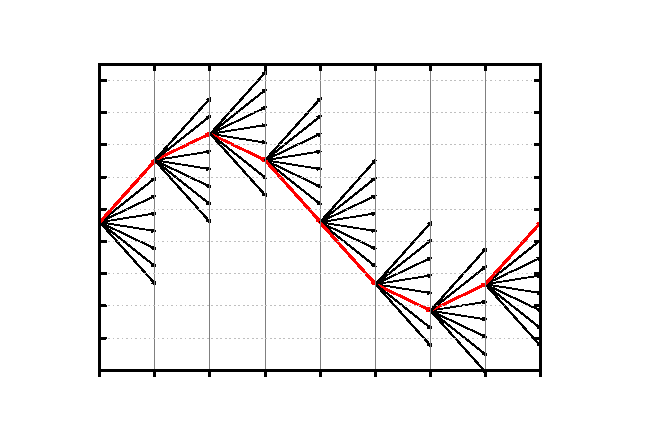
\includegraphics{RiemannCodeGenerationSineWave73_new.pdf}
%   \caption{One possible approximation of sine wave generation to get the Riemann Code}
%   \label{fig:RiemannCodeGenerationSineWave}
%\end{figure}

This sequence of slopes, referred to $i_0$ values, is:
\begin{equation}
 +7\hspace{.3cm} +3\hspace{.3cm} -3\hspace{.3cm} -7\hspace{.3cm} -7\hspace{.3cm} -3\hspace{.3cm} +3\hspace{.3cm} +7,
 \end{equation} which represents the following Riemann code:
\begin{equation}
000\hspace{.3cm} 010\hspace{.3cm} 101\hspace{.3cm} 111\hspace{.3cm} 111\hspace{.3cm} 101\hspace{.3cm} 010\hspace{.3cm} 000.
\end{equation}
\label{eq:RiemannCodeSineWave} 
   
 The Riemann Code consists of eight triplets where each triplet represent the three different switches and the number of triplets represent the number of sampling points corresponding to the \gls{ab:osr}.
This particular generated Riemann code was used to synthesize sine waves in the frequency range between \SI{500}{\MHz} and \SI{6}{\GHz}, as seen in Figure \ref{fig:7SignalsSameSlopeInOnePlot}.



\begin{figure}[htb!]
   %\centering
   \hspace{.8cm}
   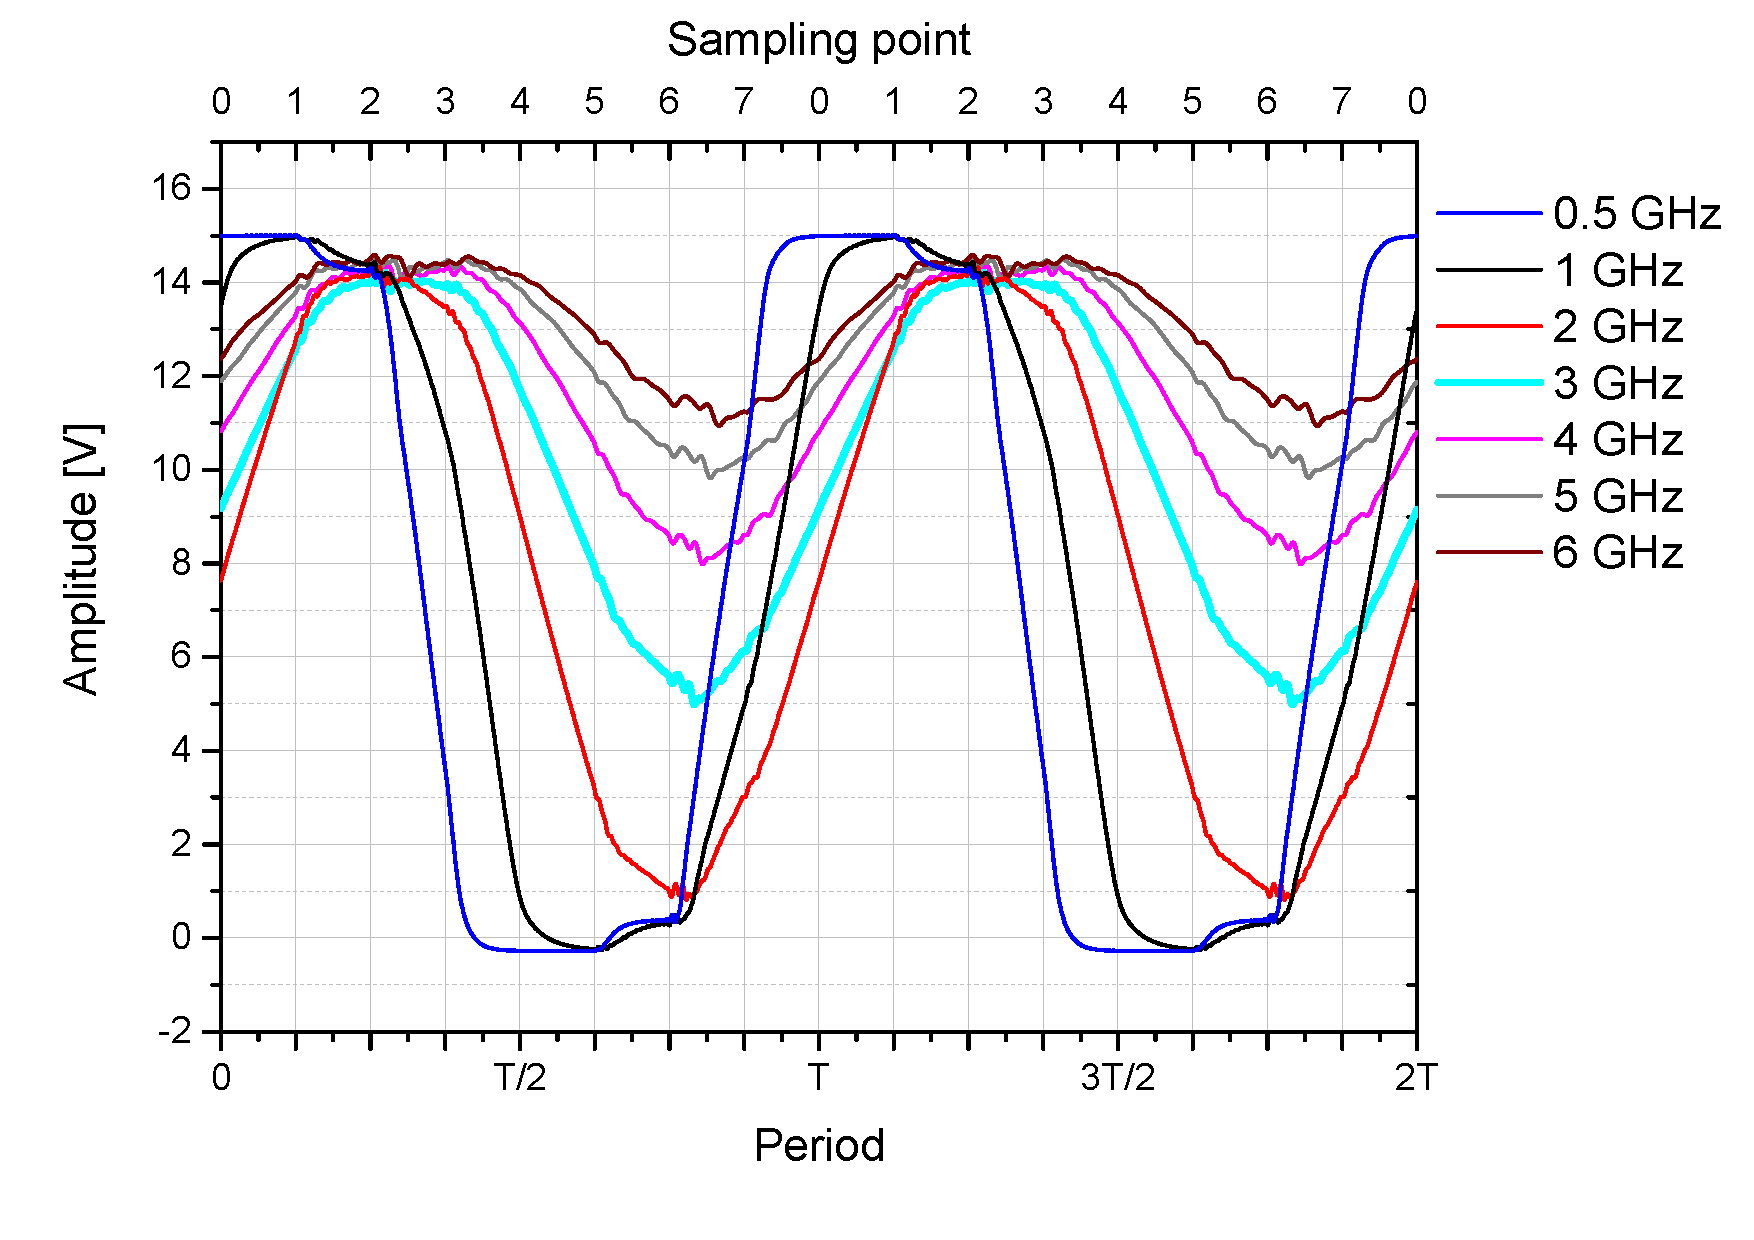
\includegraphics[width=0.75\textwidth]{Vout_sine_SigBWdifferent_SameSlope_73_PeriodT.pdf}
   \caption{Signals synthesized with demonstrated Riemann Code for the frequency range from \SI{500}{\MHz} to \SI{6}{\GHz} over two periods}
   \label{fig:7SignalsSameSlopeInOnePlot}
\end{figure}

The Figure \ref{fig:7SignalsSameSlopeInOnePlot} shows seven synthesized signals generated with the same input but with different sampling frequencies. 
Here the signals amplitude is plotted over two periods in time domain.
Due to the different absolute sampling times, the amplitude of the signals differ.
The maximum reachable amplitude is the supply voltage, here set to \SI{15}{\volt} to avoid unnecessary much heat and power losses. 
If this voltage is reached, the signal wave form is clipped and transforms the sine wave into an rectangular form.
The shape from most of the plotted functions fit fairly to the one of a theoretical sine wave.
But Figure \ref{fig:7SignalsSameSlopeInOnePlot} also highlights already some limitations of the designed circuit, as the blue curve turns into a rectangular signal form.\\

\begin{figure}[htb!]
   \centering
   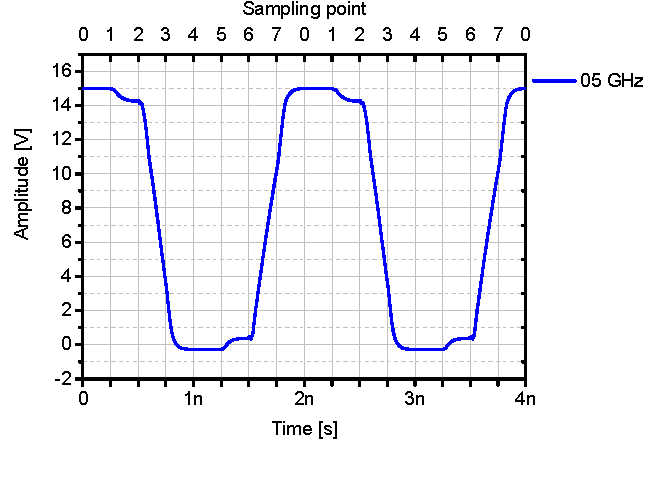
\includegraphics[width=0.75\textwidth]{Vout_sine_SigBW_05GHz_3bit_long.pdf}
   \caption{Synthesized sine wave for frequency of 0.5GHz}
   \label{fig:SineWave05GHz}
\end{figure}

The circuit designed in chapter \ref{ch:design} is optimized to cover the frequency range from \SI{1}{\GHz} to \SI{6}{\GHz} fairly well, if a voltage swing of nearly  two volts is still acceptable.
If we go beneath a frequency of \SI{1}{\GHz} the desired shape of a sine wave is going to be rectangular due to the long sampling time, refer to Figure \ref{fig:SineWave05GHz}.\\
The blue signal which should represent a sine wave with a signal frequency of \SI{500}{\MHz} is clipped and hence shows the behaviour of a rectangular signal.
 This undesired behaviour is induced from a fully charged output capacitance.
 This signal frequency is the lower bound on the frequency range for the signals for the used configuration.
%This lower bound could be shifted to even lower frequencies if the dimensions are tuned to be smaller
The upper bound on the frequency range is the signal with the at least detectable voltage swing, which could be amplified.
If at least a voltage swing of \SI{2}{\volt} is accepted, in this configuration the upper bound would be a signal frequency of \SI{6}{\GHz}.\\
% to increase this upper bound the transistor dimension have to be bigger

%%% put in the limitation here or later in a seperate paragraph???
To show how accurate the generation of the signals is, figure \ref{fig:SineWaveSynthVsTheoretical} compares a theoretical sine wave signal (red) with a synthesized one (black) for a frequency of \SI{1}{\GHz}.
The synthesized signal is same as the black curve in Figure \ref{fig:7SignalsSameSlopeInOnePlot}.
%, which within this scale already seems to turn into a rectangular signal form.
Setting up the right parameters, a good fit to a sine wave can be performed.\\
In general the sine wave is of the form: 
\begin{equation}
	v(t)= V_{DC} + \widehat{v} \cdot sin( 2  \pi  f \cdot  t + \phi).
\end{equation}
The synthesized signal (black) in Figure \ref{fig:SineWaveSynthVsTheoretical} fits pretty good to the theoretical sine wave, which has an amplitude of $\widehat{v} = \SI{7.5}{\volt}$, a signal frequency of $f = \SI{1}{\giga \hertz}$, a phase shift of $\phi = \pi / 4$ and an DC offset of $V_{DC} = \SI{7.5}{\volt}$.

\begin{figure}[htb!]
   \centering
   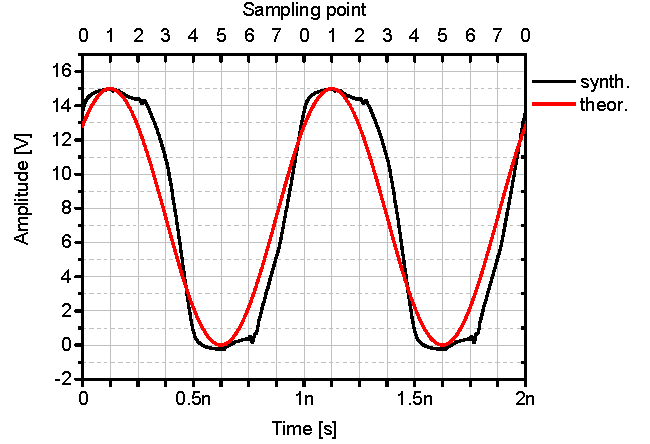
\includegraphics[width=0.75\textwidth]{Vout_SynthVsTheo.pdf}
   \caption{Synthesized sine wave with the theoretical sine wave}
   \label{fig:SineWaveSynthVsTheoretical}
\end{figure}

Although the fit seems to be very good, two distortions are visible in the peak and the valley of the synthesized signal.
($\rightarrow$\textit{Explaining these two distortions exactly for this signal frequency? Is it enough to explain some distortion at the example of 500MHz?}$\leftarrow$)
The fit is not perfect since the digital to analog conversion always introduce noise to the signal. (\textbf{refer to chapter \ref{ch:fundamentals} and the \gls{ab:sqnr}).compare to the characteristic of DAC. Which SQNR is expected, which is achieved? $\rightarrow$ plot?} \\

Figure \ref{fig:SineCompare} highlights the difference between the synthesized and the theoretical sine wave form in a more detailed way.

\begin{figure}[htb!]
	\centering
  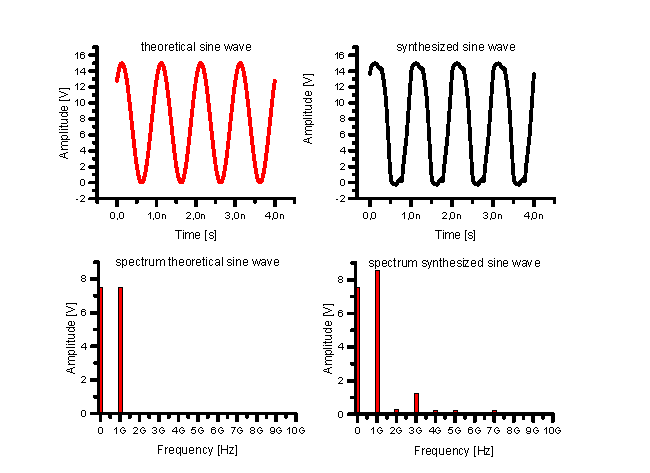
\includegraphics[width=1\textwidth]{SineCompare.pdf}
	\caption{Comparison between a theoretical and a synthesized sine wave with their spectrum}
	\label{fig:SineCompare}
\end{figure}

A sine wave is compared to the synthesized one with their corresponding spectra.
The spectra of signals are a lot easier to compare in contrast to the time domain signal with respect to the accuracy.
%The spectrum of the signal demonstrates how accurate the signal is synthesized compared to a perfectly shaped sine wave. 
Since the spectrum of a perfect sine wave only consists of a DC part and the harmonic frequency it is easy to check whether the generated signal fits to it or not.\\
On the top left side of Figure \ref{fig:SineCompare} the theoretical sine wave is plotted in red. Underneath of (the time domain signal) it the spectrum presents the frequency portion for the direct component at \SI{0} {\Hz} and a fundamental frequency portion at \SI{1}{\GHz}.
This Fourier transformation represents the frequency portions of a clear sine wave. 
The synthesized sine wave on the top right side fits fairly well to the theoretical one.
The spectrum of the synthesized signal shows nearly the same behaviour since only some harmonics distorts the signal.
Beside the direct component and the fundamental frequency component there are some additional unwanted frequency portions.
The maximum absolute distortion of this synthesized signal is about \SI{1}{\volt} in amplitude at the third harmonic at the frequency of \SI{3}{\GHz}.
 The 2nd to 10th harmonic are at most a half of a volt in absolute value of the amplitude (\textit{relative reference?}). \\
\textit{The accuracy is very good. This can be verified by the signal to noise ratio -> explain, state the SNR}


As the sampling frequency can be changed to tune the signal frequency of the output signal it is also possible to change the input control sequence to manipulate the shape of the signal.
Due to the three bit resolution there is a limited number of different slope combinations to synthesize a sine wave.
In fact there is the limit of six different combinations to synthesize the sine wave.
%For the rising edge of the upper half of sine wave, the number of slopes to synthesize is limited to two, by the fixed \gls{ab:osr} of four.
The six combination to synthesize a sine wave are: 75, 73, 71, 53, 51 ,31 with respect to the $i_0$ values.
The first digit indicates the slope of the first sampling point and the second digit respectively the second sampling point for synthesizing the rising edge of a sine wave.
%With eight different slopes representing the full spectrum between the most negative and the most positive one, exactly four slopes can represent a rising edge of a sine wave, $+7i_0, +5i_0, +3i_0, +1i_0$.
These six combinations are plotted in Figure \ref{fig:SameSigBWDifSlope} over two periods for the signal frequency of \SI{3}{\GHz}. 

\begin{figure}[htb!]
	\centering
  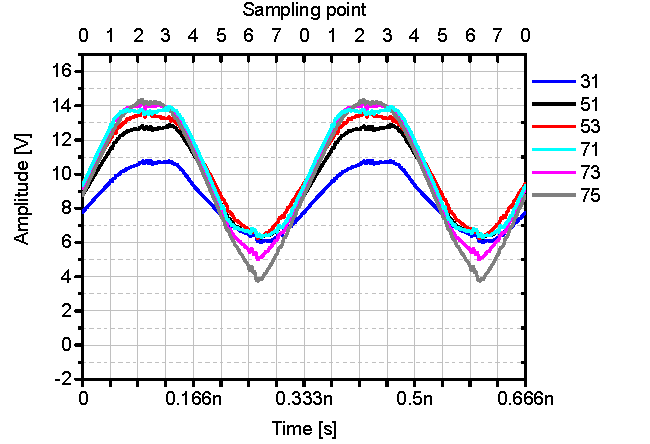
\includegraphics[width=1\textwidth]{Vout_7sine_SameSigBWdifferent_DifferentSlope.pdf}
	\caption{Signals with the same signal bandwidth but different input control}
	\label{fig:SameSigBWDifSlope}
\end{figure}

Figure \ref{fig:SameSigBWDifSlope} shows the different shapes of a sine wave for a frequency of \SI{3}{\GHz}.
This is utilized to calculate the Riemann Code which fits best to the theoretical signal.


\subsection{rectified sine wave generation in the time domain}
Based on the same approximation principle of the signal in Figure \ref{fig:SineWaveCodeGeneration}, the Riemann Code for the rectified sine is generated. 
The chosen Riemann Code for the rectified sine is:
\begin{equation}
 000\hspace{.3cm} 010\hspace{.3cm} 101\hspace{.3cm} 111\hspace{.3cm} 000\hspace{.3cm} 010\hspace{.3cm} 101\hspace{.3cm} 111.
\end{equation}
\label{eq:RiemannCodeRectSine}

Using this code a rectified sine wave is synthesized by the designed circuit.
The generation of the rectified sine wave is the same as for the normal sine wave. 
This only shows a different signal which could be synthesized.






\subsection{triangular wave generation in the time domain}
This is a triangular wave.


\section{Stability analysis of the realised circuit}
The stability and energy consumption analysis helps to get an impression/ understanding of figures and numbers of the designed circuit. Although this two aspect are of an important role for the development of a high speed \gls{ab:dac} this analysis are not complete. The whole detailed analysis could not be investigated in this thesis due to complexity and time issues, what its meaning is not to belittle. For these aspects it is important to state that the designed circuit is in no way optimized with respect to those \\
The stability analysis is important to ensure that the circuit under test do not oscillate. 
 To check this, the complex impedance at specific points in the circuit is measured.
 If the real part of the impedance is positive for the whole frequency range of the simulation, it indicates in an easy way that the circuit does not oscillate.
This simulation is done within the ADS tool. 

\section{Energy consumption analysis of the realised circuit}
If the \gls{ab:osr} is increased to get a better accuracy, the switching frequency is also increased and therefore the energy consumption.
In addition to the power consumption issue, the components have a unity current gain frequency limit.
If the resolution is increased to get a better accuracy, the whole circuit would become more complex and the energy consumption would increase.\\
Using the \gls{ab:osr} of four, we already get a sampling frequency of \SI{2}{GHz} at the lower bound.
For this reason the switches have to switch within \SI{0.5}{\nano \second} which increase the gate drive current which increase the power loss.\\
Due to the idea to use the presented topic for mobile communication it could be implemented in mobile devices, although this thesis only handles the device for the base station. If it could be used in a mobile device the energy consumption is critical.\\
The energy consumption of the designed circuit in chapter \ref{ch:design} is simulated with \gls{ab:ads}.\\
There were the trade off between the power consumption of the high side switching transistor and the switching behaviour.
Since the switching process needs to be very fast a high current is needed.
This are losses.
The driver circuit has to be optimized to reduce the energy consumption while maintaining the the switching process correctly.
If the correct hard 
\\
 For the chips used for the demonstrator refer to the work of Stephan Maroldt who states, that the power consumption is:  divided into static and dynamic ones. The switching losses are greater than the static ones.
The losses are divided into dynamic losses of the switches and static losses.
% switch voltage for on/off state, switch time, static losses and dynamic losses.

\section{Proof of concept simulation with existing components}
\label{ch:ProofOfConceptWithExistingComponents}
This simulation is based on the measurements and the design of various chips from Stephan Maroldt.
This two bit resolution simulation is done to compare the demonstrators measurements with the simulation. \textbf{two-bit resolution, osr = 4, keep it small and simple, frequency higher, demonstrator, assembly, less complex} 
The three bit resolution DAC was too complex to realize in a first approach on a hybrid substrate. Therefore an easier approach was designed to validate the proof of concept.

\section{Evaluation of the simulation results for the Riemann Pump}
Nonetheless the number of signals which can be synthesized with this particular concept is increased with the possibility to change to another combination of slopes to approximate the signal.
All this calculation should be done with a signal processor and an algorithm.
With the variation of the slopes and the variation of the sampling time in theory it is possible to create every single signal with more or less good \gls{ab:sqnr}.
\\
When the component dimensions, like the switching transistors and load impedance, are fixed it is impossible to reach a bandwidth which goes from\gls{ab:dc} to \SI{6}{\GHz}.
The issue is that a small transistor dimension could synthesize signals to a very low signal frequency but will be unable to synthesize a signal at 6GHz due to the fact that the amplitude would be too small.
Hence the signal frequency bandwidth would be shifted to the smaller frequencies. 
If the \gls{ab:osr} is increased, the sampling time is decreased and therefore the signal quality is better because we have a more accurate synthesized signal. \\
If the transistor dimension is chosen to be bigger, the higher signal frequency could be synthesized with a decent voltage swing but the low signal frequencies would turn into a rectangular shape. 
This is the trade off between the shift of the bandwidth (shifting to even higher frequencies is possible but the bandwidth is nearly constant as long the output capacitance is constant too.) The trade off for the bandwidth shift to higher frequencies is, that with the signal frequency the switching frequency is increasing linearly (for an osr; eight times) and therefore the dynamic losses are increasing with this switching frequency.
By the way the transistor switching speed is determined by the dimension of the driver circuit, so if the switching speed is increased the gate driving current has to be increased to switch the transistors.

 The presented results show the theoretical feasibility of the approach.
 In a more enhanced project a MATLAB algorithm would compute this code by minimizing the deviation between a theoretical signal and the synthesized signal.
evaluate the simulation results, what is to expect in realisation. 
What is the expectation to the measurement?
